\documentclass[preprint,12pt]{elsarticle}

% -----------------------------------------------------------------------------
% Encoding, page layout, and typography
% -----------------------------------------------------------------------------
\usepackage{placeins}
\usepackage[utf8]{inputenc}
\usepackage[T1]{fontenc}
\usepackage[a4paper, margin=1.8cm]{geometry}
\usepackage{microtype}
\usepackage{setspace}
\bibliographystyle{elsarticle-harv}
% -----------------------------------------------------------------------------
% Mathematics and algorithms
% -----------------------------------------------------------------------------

\usepackage{amsmath}
\usepackage{amsfonts}
\usepackage{nicefrac}
\usepackage{algorithm}
\usepackage{algpseudocode}

% -----------------------------------------------------------------------------
% Tables
% -----------------------------------------------------------------------------

\usepackage{booktabs}
\usepackage{threeparttable}
\usepackage{multirow}
\usepackage{makecell}
\usepackage{tabularx}
\usepackage{arydshln}
\usepackage{colortbl}

% -----------------------------------------------------------------------------
% Figures, colours, and TikZ
% -----------------------------------------------------------------------------

\usepackage{graphicx}
\graphicspath{{./images/}{./figures/}}

\usepackage{xcolor}
\usepackage{tikz}
\usetikzlibrary{positioning,calc,arrows.meta,fit,backgrounds,decorations.pathreplacing}

\usepackage[font=small]{caption}
\usepackage{subcaption}

% -----------------------------------------------------------------------------
% References, links, and notes
% -----------------------------------------------------------------------------

\usepackage{natbib}
\bibliographystyle{abbrvnat}
\setcitestyle{authoryear,open={(},close={)}}

\usepackage{xurl}
\urlstyle{same}
\usepackage[hidelinks,hypertexnames=false]{hyperref}
\providecommand{\DOIprefix}{https://doi.org/}
\providecommand{\theHpage}{\thepage}
\setlength{\emergencystretch}{2em}
\usepackage{lineno}
\usepackage{todonotes}

% -----------------------------------------------------------------------------
% Custom commands
% -----------------------------------------------------------------------------

\newcommand{\rev}[1]{{\color{red}#1}}
\newcommand{\indicator}[1]{\mathbb{1}_{\{#1\}}}

\usepackage{titlesec}

\titleformat{\section}
{\normalfont\Large\bfseries}
{\thesection}{1em}{}

\titleformat{\subsection}
{\normalfont\large\bfseries}
{\thesubsection}{1em}{}

\titleformat{\subsubsection}
{\normalfont\normalsize\bfseries}
{\thesubsubsection}{1em}{}

\titleformat{\paragraph}[runin]
{\normalfont\normalsize\bfseries}
{}{0pt}{}
\titlespacing*{\paragraph}
{0pt}{1.0ex plus 0.2ex minus 0.1ex}{0.8em}
% -----------------------------------------------------------------------------
% Document
% -----------------------------------------------------------------------------

\begin{document}
% ------------------------------------------------
% -----------------------------------------------------------------------------
% IVT-style printed cover
% -----------------------------------------------------------------------------
\begin{titlepage}
\newgeometry{top=1.65cm,bottom=1.35cm,left=2.15cm,right=2.15cm}
\thispagestyle{empty}
\rmfamily

\noindent\rule{\textwidth}{0.55pt}

\vspace{0.75cm}

\begin{center}
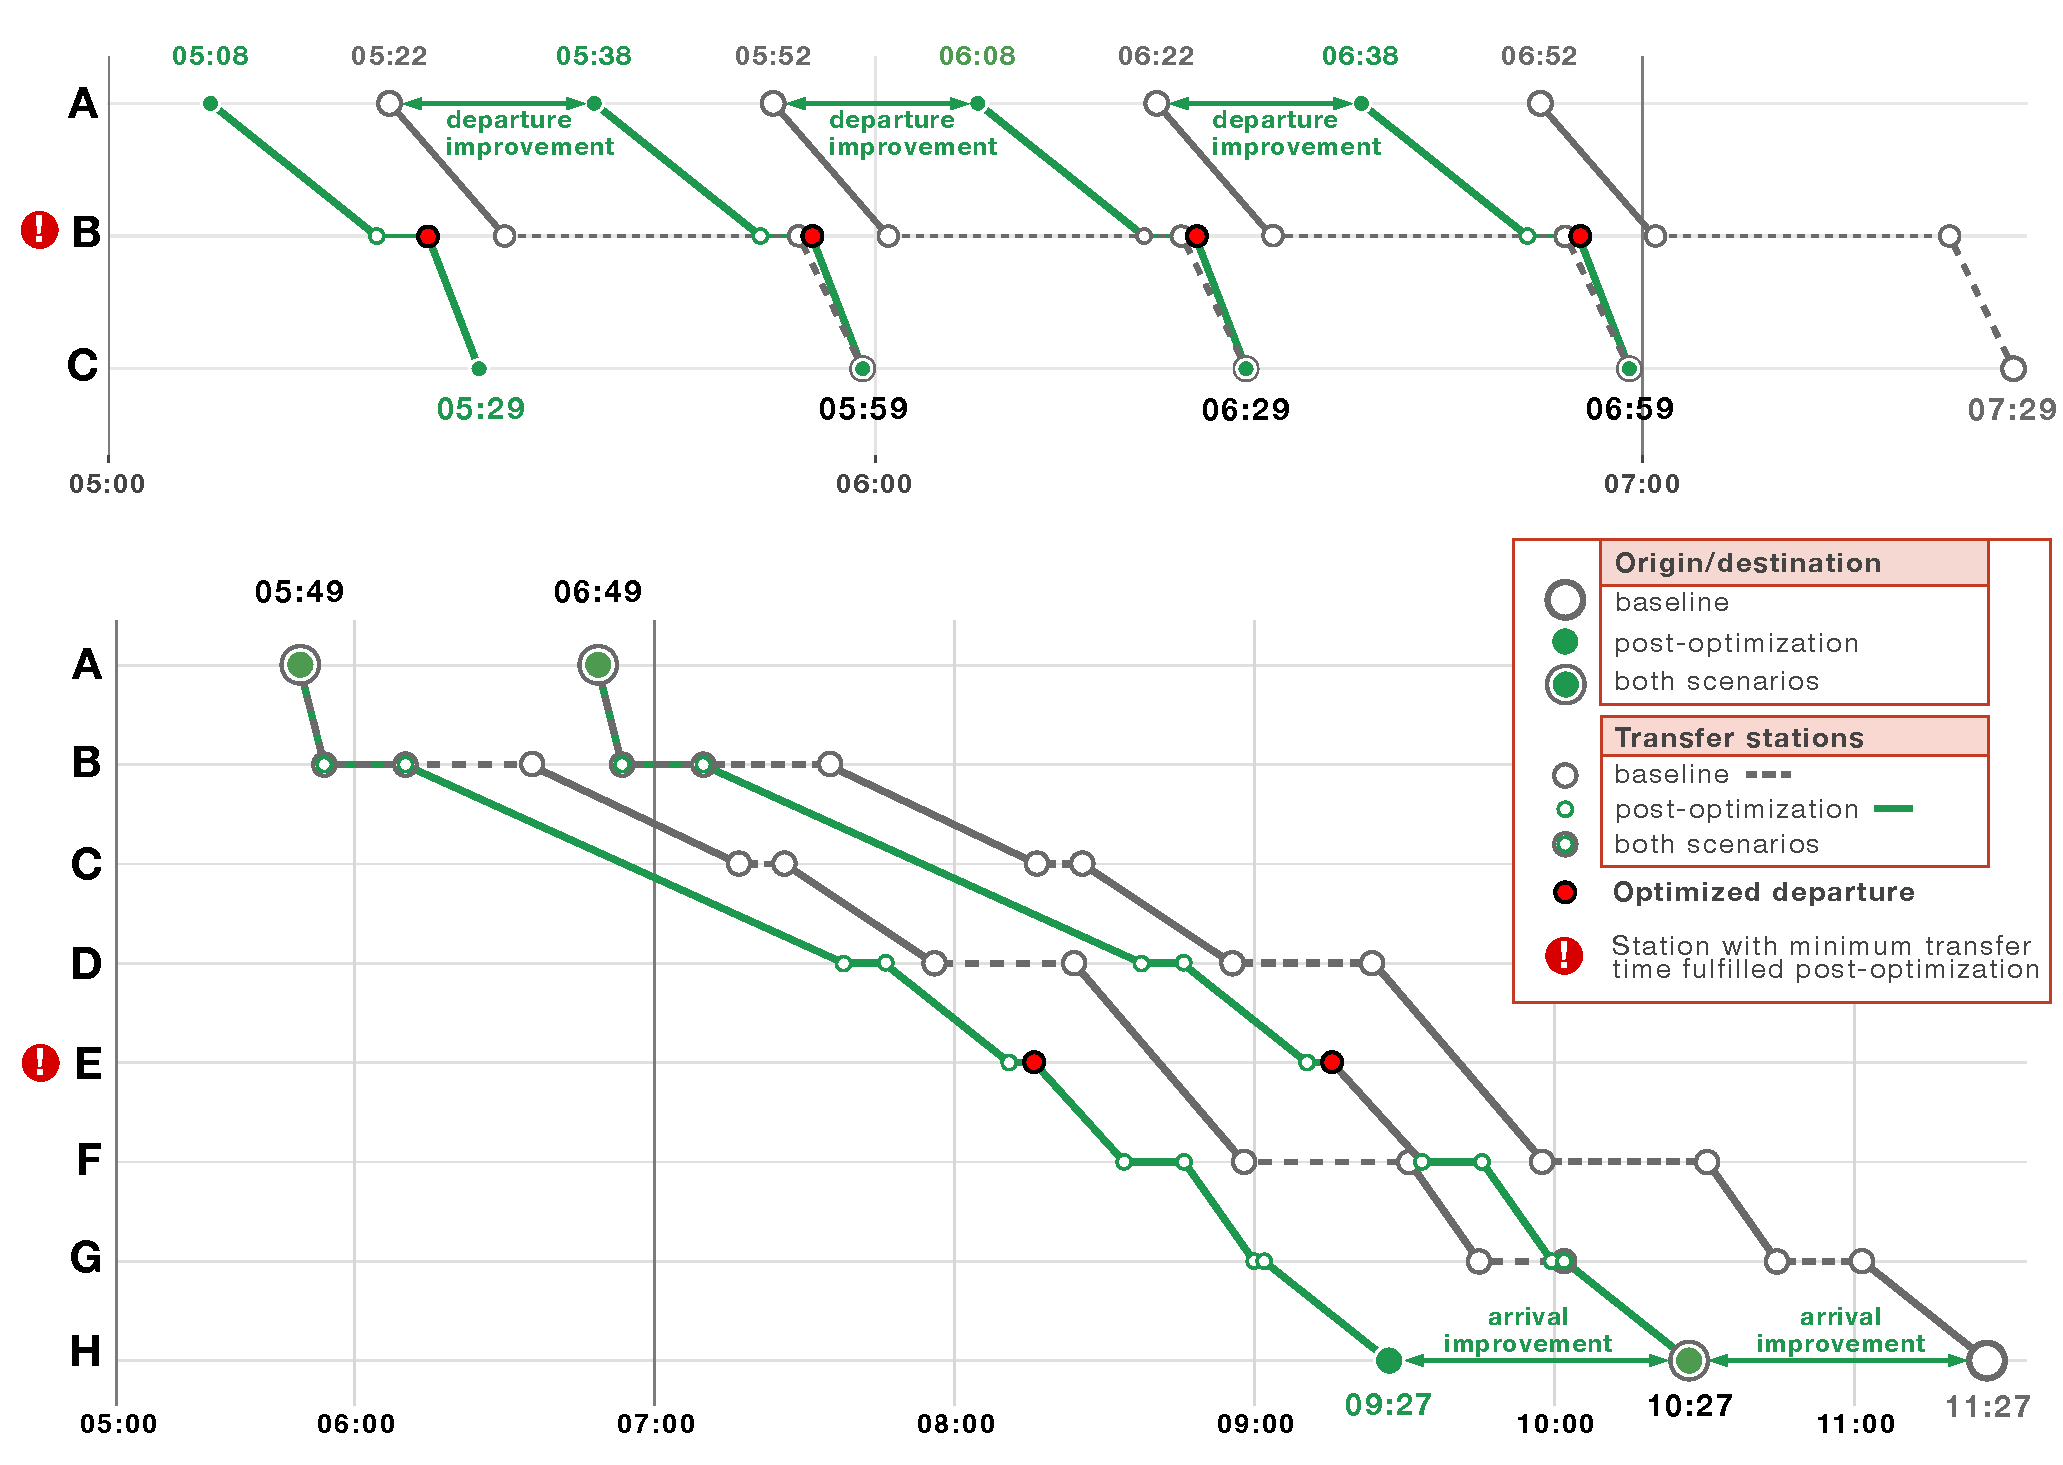
\includegraphics[
    width=\textwidth,
    height=12.55cm,
    keepaspectratio
]{figures/cover/part2_od_extreme_paths_step3_2035EASYTITLE.pdf}
\end{center}

\vspace{0.35cm}
\noindent\rule{\textwidth}{0.55pt}
\vspace{0.70cm}
\noindent
{\fontsize{18}{21}\selectfont\bfseries
Periodic Timetable Modelling \&\\[-1.15em]
Matheuristic Event-Retiming Optimization\\
of the Swiss Passenger Rail Network\par}

\vspace{0.55cm}
\noindent
{\fontsize{14}{17}\selectfont\bfseries
Student: Matthias Benjamín Andrews García\\
Scientific Head: Prof. Dr. Francesco Corman\\
Supervisors: Viera Klasovitá, Jacob Trepat Borecka\par}

\vfill
\noindent
\begin{minipage}{\textwidth}
\raggedright
{\fontsize{11.5}{14}\selectfont\bfseries Master Thesis\par}
\vspace{0.18cm}
{\fontsize{11.5}{14}\selectfont\bfseries
MSc Spatial Development and Infrastructure Systems\hfill 19-757-996\par}
\vspace{0.45cm}
{\fontsize{11.5}{14}\selectfont June 2026\par}
\end{minipage}

\vspace{0.65cm}

\noindent
\begin{minipage}[b]{0.45\textwidth}
    \raggedright
    
\includegraphics[width=0.96\linewidth]{figures/cover/ivt_logo.png}
\end{minipage}
\hfill
\begin{minipage}[b]{0.42\textwidth}
    \raggedleft
    
\includegraphics[width=0.96\linewidth]{figures/cover/eth_logo.png}
\end{minipage}

\restoregeometry
\end{titlepage}

% Blank verso page for double-sided printing.
\clearpage
\thispagestyle{empty}
\null
\clearpage

\begin{frontmatter}

% So that figures have numbers as subfigures.
\renewcommand{\thesubfigure}{\arabic{subfigure}}
\makeatletter
\renewcommand{\p@subfigure}{\thefigure.}
\makeatother

\title{Periodic Timetable Modelling \& \\ Matheuristic Event-Retiming Optimization\\
of the Swiss Passenger Rail Network}

\author{Matthias Benjamín Andrews García}
\address{
IVT,
Swiss Federal Institute of Technology\\
Stefano-Franscini-Platz 5, 8093 Zurich, Switzerland\\
E-mail: mandrews@student.ethz.ch, Student number: 19-757-996\\
June 2026}
\begin{abstract}
\setstretch{0.96}
Rail timetables translate infrastructure and service patterns into complete passenger journeys through recurring rolling, dwell, transfer, and waiting-time components. Existing research provides both long-run accessibility analyses and increasingly passenger-oriented timetable-optimization methods, but these perspectives are less often connected in one consistent, national-scale journey model. This thesis develops such a model for the Swiss passenger rail network. Part~I reconstructs historically timetabled journeys between 131 stations and evaluates them with OD-demand-weighted indicators, allowing changes across timetable years, cantons, and journey components to be compared consistently. Part~II builds detailed 2026 and 2035 station-level demand and path-allocation states across nearly 1'600 stations and tests whether small integer-minute retimings can improve passenger-weighted performance while preserving the existing timetable structure.

The methods combine compact timetable-token expansion, schedule-based routing, OD weighting, gravity modelling, iterative proportional fitting, and dominance-based allocation among retained nondominated paths. The retiming search proceeds through three increasingly targeted stages. Step~1 screens missed transfers and transfer-wait opportunities using station-board proxies; Step~2 evaluates additional candidates on paths retained under the validated Step~1 timetable; and Step~3 widens the potential candidate field and repeatedly re-scores Step~2 reference paths as compatible edits are accepted. This qualified model-based matheuristic combines a mathematically defined full-network objective and feasibility structures with heuristic candidate generation, sequential selection, exact reference-path calculations, structural validation, and full-network OD rerouting. In so doing, it focuses the computation on an interpretable local timetable neighborhood while retaining national passenger consequences as the final measure of performance.

Part~I shows that passenger-weighted timetable performance can be tracked coherently across decades by representing timetable, routing, and demand layers explicitly, while also quantifying substantial temporal and spatial variation behind national trends. In Part~II, the final corrected Step~3 timetable reduces post-departure travel by 94'216 passenger-minutes per day in 2026 and 112'419 in 2035, equivalent to passenger travel-time savings of 2.78 and 3.12 seconds per weighted trip, monetized on a national yearly scale as CHF~7.6~million and CHF~13.3~million, respectively. Most savings arise from reduced transfer and same-train dwell time; rolling time changes modestly because the proposed timetable edits maintain unchanged travel times between adjacent stations on all lines. The effects are concentrated: most OD pairs remain unchanged, while several origins and corridors experience considerable benefits alongside occasional local worsenings. The passenger-weighted mean and the network-scale daily passenger-minute objective both improve in each model year. The thesis therefore demonstrates how passenger-weighted historical measurement can support targeted timetable improvement and how carefully validated local retimings can produce measurable benefits in a periodic national clockface network.



\end{abstract}

\begin{keyword}
rail timetabling \sep periodic timetabling \sep schedule-based routing \sep passenger-weighted accessibility \sep matheuristics

\end{keyword}

\end{frontmatter}

% Uncomment if line numbering is needed for review.
% \pagewiselinenumbers

% -----------------------------------------------------------------------------
% Front matter lists
% -----------------------------------------------------------------------------
\pagenumbering{roman}

\setcounter{page}{1}
\clearpage
\tableofcontents

\clearpage
\phantomsection
\addcontentsline{toc}{section}{List of Figures}
\listoffigures

\clearpage
\phantomsection
\addcontentsline{toc}{section}{List of Tables}
\listoftables

\clearpage

\pagenumbering{arabic}

\setcounter{page}{1}
\section{Introduction}\label{sec:intro}

\subsection{Motivation}\label{sec:motivation}
Swiss rail planning is often discussed through infrastructure: new base tunnels, capacity projects, rolling stock, station expansions, and national programmes such as Bahn 2000 and STEP 2035. Yet for passengers, much of the railway's changing usefulness is experienced not only through infrastructure upgrades, but also through timetable updates. A five-minute reduction in transfer time at a hub, a new systematic half-hourly pattern, or a previously missed connection that becomes feasible after a one-minute shift can generate meaningful passenger-time benefits, especially when the affected connection is repeated throughout the day and used by many travellers. In a regular-interval railway, the passenger experience is a property of the entire time--space network: train movements, station dwell times, waiting times, and transfer times recur throughout the service day.

This thesis studies the evolution of this time--space network in the Swiss rail system across the past, present, and future. Its first objective is descriptive: to reconstruct how timetable-realized rail connectivity has evolved historically and how it differs across cantons and stations. Its second objective is prescriptive but deliberately conservative: to test whether small integer-minute timetable retimings can reduce passenger-weighted travel-time burdens while preserving rolling times and transfer feasibility. Instead of rebuilding the full national timetable from the ground up, Part~II uses a model-based matheuristic: heuristic candidate generation and sequential selection are combined with mathematical formulations, exact route calculations, structural validation, and full-network evaluation. The global target remains the complete-network minimum of passenger-weighted post-departure OD travel time; the implemented search approaches this target within a restricted, interpretable neighborhood of the existing timetable rather than solving all event times and passenger paths simultaneously.

The Swiss case is well-suited to this question. The network is dense, transfer-oriented, and structured around regular intervals on most major lines. The timetable is therefore suitable for representation at an abstracted hourly or two-hourly interval level. Nevertheless, a change at one station may improve one transfer while damaging another. A useful optimization method must therefore distinguish locally promising changes from system-level effects. This thesis does so through the use of passenger-weighted OD paths, to avoid the simplistic effects of relying on unweighted adjacent geometries alone.

\subsection{Research questions}\label{sec:research-questions}

The thesis is structured around two research questions.

\begin{description}
    \item[RQ1] (Addressed in Part I) How can historical Swiss rail timetables be converted into comparable, passenger-weighted measures of rolling, dwell, transfer, waiting, and total journey time, and how do these measures vary over time and across cantons?

    \item[RQ2] (Addressed in Part~II) Can a modelled matheuristic identify small integer-minute event shifts in the 2026 and 2035 timetables that reduce total passenger-minutes while preserving the structure of the existing timetable?
\end{description}

The second question concerns pinpointed improvements to baseline timetables rather than a global timetable optimization from the ground up. Dense railway timetabling is combinatorial and highly constrained. The major contribution of this thesis is therefore in documenting a reproducible way to identify and verify a targeted set of local retimings of a preexisting national timetable.
\subsection{Contributions}\label{sec:contributions}

The thesis makes three main contributions.

First, it constructs a historical timetable-analysis pipeline for 131 selected Swiss stations. The pipeline combines reconstructed digitized historical timetables, a 2023 NPVM-derived passenger-demand anchor, population-scaled marginal totals, generalized-cost skims, and iterative proportional fitting. This produces an OD-weighted analysis of how timetable-realized journey-time components have evolved historically.

Second, it develops a more detailed station-level model for the 2026 and 2035 timetables. This model stores all retained nondominated paths for each OD pair in a two-hour reference window, including complete intermediate stop timings, transfer events, rolling, dwell, transfer, and waiting components, and path-allocation information. It therefore makes it possible to move from aggregate OD matrices to individual train services, transfer pairs, and adjacent line segments. The model is combined with a station-level demand representation based on SBB passenger-frequency constraints, station population, service intensity, calibrated gravity terms, IPF balancing, and a transfer-throughput correction.

Third, it introduces a three-step, model-based matheuristic for timetable retiming. Step~1 selects candidate shifts from high-flow line transfers and station-board near misses, Step~2 expands the search using exact current-route scans based on the validated Step~1 timetable, and Step~3 broadens the search context to capture additional local improvements and review the combined result. The final Step~3 timetable reduces post-departure passenger-minutes in both 2026 and 2035. The benefits are modest when averaged across the network but substantial for selected OD pairs, demonstrating that targeted retiming of an existing national timetable can produce measurable passenger-weighted improvements.

\subsection{Scope and exclusions}\label{sec:scope}

This thesis excludes from consideration the requirements and effects of rolling-stock circulation, crew schedules, platform occupation, line-capacity constraints, stochastic delay propagation, fares, or competing mode choices such as private car travel. The status quo timetable is used as the operational baseline, and the optimized scenarios apply only small integer-minute retimings to selected sections. At the level of abstraction used in this thesis, rolling-stock circulation, crew availability, and related operational requirements are therefore assumed not to differ substantially between the baseline and optimized scenarios. However, the proposed alterations would still require further operational validation, especially with respect to platform occupation and local capacity constraints.

The thesis also does not claim that the modelled demand is fully representative of observed real-world demand, nor that all future induced-demand effects by 2035 are captured. In the 2035 demand model, population growth and service-improvement effects are approximated through exogenous scaling and a calibrated accessibility/service uplift before balancing, but this is not sufficient to fully predict 2035 demand. The optimized timetable comparison therefore holds demand fixed within each year and scenario comparison so that the effect of timing changes can be isolated.

The analysis is therefore best understood as a passenger-weighted timetable and transfer-efficiency study rather than a timetable plan rebuilt from the ground up. A globally optimized timetable of the same scale would require additional constraints, compute power, and validation steps beyond the intended scope of this thesis.
\clearpage

\section{Literature review}\label{sec:litreview}

This thesis sits at the intersection of three strands of transport research. The first concerns accessibility and the passenger-facing quality of rail service: how much useful movement a timetable makes possible, and how this changes when travel time, frequency, waiting, and transfers change. The second concerns OD demand construction, where observed or modelled marginal information must be converted into station-to-station flow weights. The third concerns public-transport routing and timetable optimization, especially periodic timetables and transfer synchronization. The present literature review follows the order of the thesis: Part~I reconstructs historical passenger-weighted timetable performance, while Part~II searches for small timetable retimings and evaluates them through full OD path rebuilding.

\subsection{Accessibility, timetable quality, and passenger experience}\label{sec:reviewaccess}

Accessibility research provides the conceptual basis for interpreting railway timetables as more than lists of train movements. In Hansen's classic formulation, accessibility expresses the potential of opportunities for interaction, rather than simply the physical extent of a transport network \citep{hansen1959accessibility}. Later reviews place this idea in a broader framework in which accessibility depends jointly on land use, transport impedance, temporal constraints, and individual or group characteristics \citep{geurs2004accessibility}. For rail timetable analysis, the most relevant implication is that infrastructure and service supply matter through the journeys they make possible: a new line, shorter headway, or better transfer is meaningful because it changes the generalized cost of reaching destinations.

The accessibility literature also warns that the chosen measure determines the interpretation. Cumulative opportunity measures, gravity-based potential accessibility, generalized-cost indicators, and person-based measures each emphasize different parts of the land-use and transport relationship \citep{geurs2004accessibility}. This thesis works with timetable-realized travel-time indicators rather than with a full opportunity catalogue. That choice is appropriate for the research questions because the empirical object is the railway timetable itself: the analysis asks how long station-to-station journeys take, how those times are composed, and how passenger-weighted outcomes change when the timetable changes.

Swiss accessibility research has shown how strongly these measures depend on the representation of the transport network and on the temporal scale of the analysis. Studies of Swiss municipalities trace long-run changes in accessibility over the second half of the twentieth century and show that improved transport supply can reshape the relative position of regions without affecting them uniformly \citep{froehlichTschoppAxhausen2005Accessibility}. Extending this historical perspective, \citet{axhausen2011swissaccessibility} analyse Swiss accessibility since 1850 and emphasize that accessibility gains are spatially uneven and linked to the changing structure of the transport system. This is directly relevant to Part~I of the thesis, where national mean improvements coexist with local reversals after specific timetable and infrastructure changes.

The Swiss case is especially suitable for a timetable-based interpretation of accessibility because the national passenger rail system is organized around coordinated recurring services. A station can become more accessible through a faster line, a shorter transfer, a higher service frequency, or simply a better timed pulse at a faraway interchange hub. These mechanisms are not equivalent from an operational perspective. A rolling-time reduction may reflect infrastructure or stopping-pattern changes; a dwell reduction may reflect a different through-service structure; a transfer-time reduction may reflect improved synchronization; and a pre-departure average waiting-time reduction may reflect increased frequency or dominance over the clockface cycle. This decomposition of travel time into its individual components is therefore treated as a central part of this thesis' analysis, allowing the reported results to distinguish not only where travel-time improvements occur, but also how they arise within the journey structure.

A second branch of the literature concerns how passengers value the components of public-transport travel. Values of time are not limited to in-vehicle movement: waiting, transfer time, reliability, and service quality can carry different weights in behaviour and appraisal \citep{wardman2004values}. Demand studies also show that public-transport use responds to service quality, including frequency and journey time, alongside fares and income \citep{paulley2006demand}. In this thesis, these findings motivate component reporting rather than a new behavioural valuation model. Rolling time, same-train dwell time, transfer time, and initial waiting are reported individually in Part~I and Part~II because each component has a different operational meaning and a different interpretation from the passenger perspective.

This component-based view also clarifies the scope of the thesis. Part~I treats accessibility operationally, as passenger-weighted station-to-station travel conditions observed through the timetable. Part~II holds demand fixed within each model year so that scenario differences can be attributed to retiming, route recomputation, and path-share changes. The literature therefore supplies the interpretation of accessibility and service quality, while the thesis focuses on the timetable mechanisms through which these quantities are realized.

\subsection{OD matrices, spatial interaction, and matrix balancing}\label{sec:reviewodmatrices}

Passenger-weighted timetable analysis requires an OD matrix, but the available observations rarely correspond exactly to the spatial level at which timetable paths are evaluated. Spatial-interaction and gravity models provide one long-established way to construct such matrices. Entropy-based formulations show that gravity-like trip distributions can be derived by maximizing the number of feasible trip configurations subject to marginal and cost constraints \citep{wilson1970entropy}. More general spatial-interaction work shows that destination attractiveness, origin size, and impedance terms can be combined in several ways depending on the behavioural and spatial assumptions of the application \citep{fotheringham1983CompetingDestinations}. In this thesis, these ideas appear in two different forms: Part~I starts from an external national OD anchor, while Part~II constructs a station-level gravity-shaped seed before imposing station-throughput constraints.

The key modelling issue is which information a gravity model is asked to provide. If observed OD flows are available at the desired spatial scale, the gravity model can be a calibration or projection device. If only marginals or station-level totals are available, the gravity model supplies a structured prior over OD pairs. That prior should then be constrained by stronger external totals where they exist. This distinction is central to Part~II: the gravity seed is used to distribute relative station-to-station demand plausibly, while the final station totals are imposed later through transfer-corrected balancing.

Matrix balancing is the corresponding statistical and computational problem: once a provisional matrix exists, its rows, columns, or station marginals must be adjusted to match trusted totals. Iterative proportional fitting has a long statistical history, including early work on adjusting sampled frequency tables to known marginal totals \citep{demingStephan1940IPF} and later formalization for contingency-table estimation \citep{fienberg1970IPF}. Closely related matrix-scaling results show the conditions under which positive matrices can be scaled to specified marginal structures \citep{sinkhorn1964MatrixScaling}. These foundations are useful because they separate two roles of a matrix: the seed matrix describes the relative pattern of trips, while balancing imposes external marginal information.

This separation also makes the limitations visible. Balancing can force a matrix to match marginals, but it cannot create information that is absent from the seed. If the seed overstates short urban trips, understates peripheral relations, or misses a cross-region pattern, IPF preserves that structure as far as the marginals allow. For that reason, both Part~I and Part~II demand layers in the thesis document the seed construction before the balancing step. The final OD matrices are used as passenger weights for timetable analysis, not as independent forecasts of all Swiss rail demand.

Part~I uses this distinction to combine a zone-level NPVM-derived OD anchor with station-level timetable paths. Zone flows are allocated to stations, adjusted for selected same-agglomeration cases, projected across historical timetable years through a generalized-cost pivot, and then balanced through IPF in Section~\ref{sec:methods-part1-ipf}. Part~II uses similar logic at a much higher resolution, with more than ten times as many stations per scenario. Observed SBB station-frequency data and estimated fallback throughputs define station constraints, while a gravity-shaped pre-balancing matrix supplies the relative OD pattern before the final transfer correction and IPF balancing in Sections~\ref{sec:methods-part2-demand-seed}--\ref{sec:methods-part2-demand-balancing}. The literature clarifies why the seed structure and the marginal constraints should be documented separately.

The OD matrices in this thesis are therefore best understood as weighting layers for timetable comparison. In Part~I, they allow historical timetables to be compared with passenger-weighted indicators rather than with unweighted station-pair averages alone. In Part~II, they ensure that the Baseline, Optimized Step~1, Optimized Step~2, and Optimized Step~3 timetables are evaluated with the same year-specific passenger weights. This fixed-demand convention is necessary for an unambiguous interpretation of small retimings, because scenario-dependent OD matrices would otherwise entangle timetable effects with demand-generation assumptions. The demand layer still plays a decisive role for Part~II by determining where small timetable changes have the greatest passenger-weighted relevance.

\subsection{Schedule-based routing and public-transport assignment}\label{sec:reviewrouting}

Public-transport assignment differs from road assignment because passengers choose not only a route through a network, but also a sequence of services with waiting and transfer consequences. Classical transit assignment introduced the idea of strategies or hyperpaths, where passengers may choose among attractive services rather than committing to a single deterministic path before arrival \citep{spiessFlorian1989OptimalStrategies}. Large-scale transit assignment work extended this perspective to equilibrium and network loading problems \citep{nguyenPallottino1988TransitAssignment}. Schedule-based models go further by representing actual departure and arrival times, which makes transfer feasibility and time-dependent path choice central to the assignment problem \citep{nuzzoloRussoCrisalli2001ScheduleAssignment}. Reviews of transit route-choice modelling emphasize that route choice can depend on in-vehicle time, waiting, transfers, reliability, information, and traveller heterogeneity \citep{liuBunkerFerreira2010Review}.

The routing layer of this thesis uses a complex custom version of typical schedule-based logic. In the data preparation and methods chapters, timetable tokens are defined and then expanded into concrete events, feasible transfer edges are created from minimum-transfer rules, and retained paths are selected by lexicographic route search. Importantly, demand is then allocated across retained alternatives according to the proportion of their respective dominance period. This allocation rule is applied consistently: for each OD pair and timetable state, the retained path alternatives, their departure coverage within the two-hour repeating clockface cycle, and their rolling, dwell, transfer, and waiting components can be accessed directly.

The dominance-minute rule is highly compatible with the Swiss structure of a periodic railway timetable. In a clockface system, a path alternative covers a regularly repeating portion of the departure-time cycle. A path that dominates many query minutes receives a proportionally larger share of the daily OD demand than a path that is available only in a narrow interval. This serves as a schedule-based deterministic equivalent to passenger-based assignment: passenger weights are distributed among the timetable opportunities available within the representative cycle, while the OD matrix remains fixed at the station-pair level.

This routing convention is especially important for Part~II. A one-minute retiming may change a transfer interval, but it can also change which paths are retained and how much of the clockface departure window each path dominates. The final validation objective of post-departure travel time defined in Section~\ref{sec:methods-part2-optimization-objective} is not directly influenced by pre-departure waiting-time changes alone, only by their potential downstream effects after boarding. Retimings therefore require rebuilding the path set and reallocating fixed OD demand across the resulting alternatives. This is consistent with the schedule-based assignment literature, which shows that timetable changes matter through their effects on feasible passenger paths, waiting conditions, transfers, and route allocation.

\subsection{Periodic timetabling and transfer synchronization approaches}\label{sec:periodic-timetabling}

Periodic timetabling provides the mathematical background for the Swiss clockface setting studied in Part~II. The Periodic Event Scheduling Problem (PESP) represents recurring events and periodic temporal constraints in a compact form \citep{serafini1989periodic}. In railway applications, PESP-style models can encode running times, dwell times, headways, turnarounds, and transfer constraints through periodic event-time differences \citep{liebchen2007pesp}. Further work on cyclic timetabling studies the underlying graph structure and cycle constraints that make such models powerful but computationally demanding \citep{liebchenPeeters2009CycleBases}. Reviews of train timetabling distinguish nominal and robust formulations and show that the operational problem quickly grows when realistic constraints are added \citep{cacchianiToth2012Timetabling}; exact and heuristic work on robust PESP makes the same point for periodic instances \citep{goerigk2015RobustPESP}.

The periodic formulation is attractive because it expresses timetable regularity directly. A train that leaves at minute 03 each hour can be represented by one periodic event rather than by every daily departure separately, while wrap variables account for movements across the period boundary. At the same time, the compactness of the periodic representation does not remove the combinatorial structure of the problem. Transfer arcs, minimum dwell times, headways, line interactions, and robustness requirements all add constraints. For a dense national network, this creates a tension between model completeness and computational tractability.

Transfer synchronization is a central passenger-facing part of this field. Fixed-interval timetable research shows that reducing waiting times at transfer points can be formulated as an optimization problem over coordinated recurring services \citep{nachtigallVoget1997FixedInterval}. Related public-transport synchronization work seeks timetables that maximize feasible or attractive transfers between lines \citep{cederGolanyTal2001Synchronization}. These studies are close to the practical motivation of Part~II: small changes in scheduled arrivals and departures can unlock a missed transfer or reduce a repeated transfer wait throughout the operating day.

Passenger-oriented periodic timetabling extends this idea by including routing or passenger costs directly in the timetable model. \citet{schiewe2020integrated} make the central argument for this integration: passenger routes depend on the timetable, so a timetable that is optimized with fixed or externally computed routes can be suboptimal once passengers are routed again. Their approach combines periodic timetabling and passenger routing, and introduces exact preprocessing together with heuristic passenger reductions so that upper and lower bounds can be traded against computation time. This is close to the logic used later in Part~II: timetable changes are not assessed only as event-time changes, but by their effect on routed passenger paths.

Recent work develops this passenger-oriented direction through several algorithmic strategies. \citet{martinIradiRopke2022Matheuristic} formulate a periodic and symmetric train-timetabling problem with integrated passenger routing on a time--space graph. Their column-generation-based matheuristic solves an LP relaxation in which columns represent train paths of a line, adds violated constraints by separation, uses Benders' optimality cuts to connect passenger travel time to the timetable, and applies large-neighborhood search and random iterative improvement to find integer solutions. The reported case concerns a morning rush-hour regional railway network in Denmark. Despite the substantial differences in solution methodology, the study adopts the same passenger-oriented premise as this thesis. Passenger routing is not treated as a post-processing step but as a central component of timetable evaluation, with passenger travel times feeding back into the assessment of timetable quality.

The same trend appears in recent benchmarking and integrated-planning work. \citet{schieweGoerigkLindner2023TimPassLib} present TimPassLib as a benchmark library for integrated periodic timetabling and passenger routing, motivated by the growing need to compare algorithms on common instances. This is an important development because it treats integrated passenger routing as a distinct computational problem rather than as a minor extension of PESP. \citet{yaoEtAl2023IntegratedStopPlanning} extend the integration further by combining network periodic train timetabling, stop planning, and passenger routing in a periodic time--space network and solving the resulting model with an ADMM-based algorithm. These examples show that the current literature is moving toward formulations in which passenger assignment, stopping patterns, and periodic timetable feasibility are optimized together, but also toward solution methods that decompose, relax, or otherwise structure the problem to keep it computationally manageable.

The demonstrated scale of decomposition-based railway models depends strongly on the level of representation. \citet{leutwilerCorman2022LogicBenders} apply logic-based Benders decomposition to a microscopic SBB timetable-planning case covering the Zurich--Luzern--Chur triangle over nine hours. The case contains 361 trains, 3’280 scheduled stops, 865 transfer connections, 955 infrastructure blocks, 45 routing areas, 5’441 route alternatives, 47’588 resource conflicts, 78’758 event nodes, and 654’823 ordering decision variables. The converged Benders iterations certify the solution of the stated microscopic formulation, and it substantially improves scalability relative to centralized benchmarks. Its focus is exact microscopic train scheduling over infrastructure resources, routes, orders, and conflicts, as opposed to macroscopic station-node coverage, OD routing, or schedule retiming. 

\citet{trepatBoreckaEtAl2025Geographic} subsequently build on this logic-based Benders framework by studying how geographic decomposition choices affect the computational performance of microscopic railway timetable planning. Their results show that the partition of the network is itself an important algorithm-design decision, with different decompositions producing substantial runtime differences: smaller subproblems are not always better. More, smaller areas reduce local subproblem effort but increase the number of boundary interactions that the global algorithm must coordinate. Fewer, larger areas make each subproblem harder but can reduce coordination overhead. Decomposition helps only when the boundaries align sensibly with the interactions that dominate the problem.

Passenger-oriented Benders models have so far been applied to much smaller station scales. \citet{yaoEtAl2025HybridBenders} combine Benders decomposition and column generation for hybrid-periodic timetabling, rolling-stock circulation, and passenger routing. Their Lower Saxony case contains 34 stations, 70 directed sections, a one-hour periodic timetable with 20 train services, and 836 time-dependent passenger groups over a six-hour scheduling horizon; in the large-case experiments, the most difficult reported instance retains an 8.6\% optimality gap after the six-hour computation limit. These two studies therefore demonstrate different forms of scale: the Zurich-Luzern-Chur case is large in microscopic infrastructure detail, while the Lower Saxony case is smaller spatially but integrates passenger routing directly into the optimization. Together, they show that decomposition can materially improve compute time, while their regionally-limited spatial extent makes clear why globally-optimal integrated formulations at the nationwide station and OD scale of this thesis are currently beyond routine computational reach without significant research advances.

Taken together with the earlier passenger-oriented and benchmark-library work, these examples show that the literature is advancing along complementary dimensions: integrated passenger-routing formulations are becoming more explicit, while decomposition-based methods are being used to manage the resulting computational scale. Concurrently, the reported applications suggest that large integrated railway models are difficult to solve, especially when passenger routing, timetable flexibility, and detailed operational constraints are combined. 

This modern literature provides the closest methodological reference point for Part~II. The thesis adopts the same passenger-oriented premise: a retiming is valuable only if it improves the passenger paths produced by the timetable. The Swiss network and the available timetable data, however, lead to a different implementation. Part~II starts from the existing national clockface timetable, restricts decisions to small rolling-preserving section shifts, and links each edit to passenger consequences through candidate generation, station-board screening, reference-path scoring, sequential compatibility checks, and full OD rerouting.

The distinction between mathematical programming, metaheuristics, and matheuristics is important. Mathematical-programming approaches formulate decision variables, objectives, and constraints explicitly and use methods such as LP, MIP, or MILP to seek optimal solutions or computable bounds. Metaheuristics provide higher-level search strategies, such as large-neighborhood or evolutionary search, that explore difficult solution spaces without embedding every interaction in one exact formulation. Matheuristics combine these traditions by using mathematical models or mathematical-programming techniques as substantive components of a heuristic algorithm \citep{boschettiManiezzo2022Matheuristics}. Formal objectives, constraints, relaxations, exact subproblems, or mathematical evaluations can thus guide a broader search, but cannot claim that the complete problem is solved to global optimality.

The scale of Part~II is most clearly expressed by the expanded daily timetable and passenger-routing state. Summed across the two considered years, the final scenario representations contain 3'171 stations and roughly 5 million possible directed station pairs, 28'283 train-service runs, and 606'899 station arrival or departure events in the 05:00--23:59 window, equivalent to about 300'000 scheduled stops. These values far exceed not only the 34 stations, 1'122 possible directed station pairs, and 20 hourly train-service runs reported in the Lower Saxony case by \citet{yaoEtAl2025HybridBenders}, but also the 3'280 scheduled stops and 361 train-service runs reported by \citet{leutwilerCorman2022LogicBenders}, whose complexity lies in microscopic infrastructure blocks and train conflicts. The reviewed passenger-oriented Benders decomposition studies therefore do not demonstrate comparable timetable-event and OD-pair scale, ruling out a globally optimal integrated approach for the purposes of this thesis in favour of matheuristics.

The implemented optimization workflow of this thesis is consequently described as a qualified model-based matheuristic decomposition. It combines the global objective of minimizing full-network passenger-weighted post-departure OD time, a binary linear formulation of candidate selection, PESP-inspired activity constraints, heuristic candidate generation, sequential acceptance, exact calculations on retained reference paths, structural timetable validation, and full OD rerouting of completed scenarios. The formulations define the target, admissible edits, incompatibilities, and passenger-benefit measures; the sequential selector searches the resulting local neighborhood without solving the complete binary selection problem as one MIP or MILP. Unlike a generic metaheuristic, the search is neither unconstrained nor a stochastic exploration of arbitrary timetables. Every candidate is a formulated rolling-preserving section shift, and every completed scenario is tested on the full station-level passenger network. The accepted set therefore constitutes a validated improvement over the baseline at a reasonable computational cost, with the explicit trade-off that global optimality cannot be claimed.


\subsection{Positioning of this thesis}\label{sec:reviewgaps}

Taken together, the reviewed literature positions the thesis as a reproducible passenger-oriented modelling and timetable-optimization workflow for Swiss passenger rail timetables. It connects accessibility measurement, OD matrix construction, schedule-based routing, and passenger-oriented retiming through successive modelling and optimization stages, reflecting the decomposition-based strategies commonly adopted for large-scale timetable-planning problems. The contribution is the integration of these techniques into a complete Swiss network measurement-and-retiming workflow whose final scenarios are evaluated across the complete modelled OD system.

Three aspects distinguish this implementation. First, the thesis evaluates modelled timetable-realized journeys rather than only infrastructure supply or abstract generalized costs, making it possible to identify whether changes arise from faster movement, reduced same-train dwell, shorter transfers, or altered waiting patterns. Second, the OD weighting is explicit: Part~I uses an NPVM-derived anchor and Part~II uses station-throughput constraints, while both separate the demand-weighting layer from the timetable/path layer. Third, the optimization procedure is organized as a sequence of increasingly refined search steps, each narrowing the planning space to a smaller set of promising timetable edits that are subsequently evaluated through full-network passenger rerouting. This structure also links the two parts of the thesis. Part~I shows that national timetable improvement is uneven across space and across time components. Part~II takes this into a prospective setting by searching for small retimings where specific transfer or routing structures create measurable passenger-minute losses. The themes of the literature review therefore reappear throughout the methods chapters: accessibility provides the interpretive framework, OD modelling provides the demand weights, schedule-based routing provides the path structure, and periodic timetabling provides the matheuristic framework for small retiming edits.

The already highly coordinated Swiss clockface timetable provides a setting in which many potential improvements occur at the scale of minutes near transfer margins rather than through ground-up timetable redesign. A workflow that can identify such changes, explain them through passenger-weighted mechanisms, and evaluate them through full OD rerouting therefore provides a practical means of assessing targeted timetable refinements at network scale. The results should be interpreted as evidence of the network-wide effects of such refinements under fixed demand and preserved rolling times.


\section{Data preparation}\label{sec:dataprep}
This chapter introduces the shared data structures and modelling conventions used in both parts of the thesis. It first describes the timetable sources and the difference between the historical Part~I representation and the optimization-oriented Part~II representation. It then defines the compact timetable-token logic used to encode periodic arrival and departure times before introducing the path-component representation used to decompose passenger journeys into rolling, dwell, transfer, waiting, and total post-departure time. These definitions provide the common basis for the historical timetable analysis in Part~I and the retiming analysis in Part~II.

\subsection{Periodic timetable data}\label{sec:data}
The periodic timetables used in this thesis are based on publicly available network diagrams created by SMA und Partner for several years between 1982 and 2026 \citep{smaPartnerDownloads}, as well as the 2035 network graphs published by the Swiss Federal Office of Transport as part of the STEP 2035 infrastructure expansion project \citep{bav2021as2035} valued at approximately CHF 16 billion \citep{sbbStep2035}.
\begin{table}[htbp]
\centering
\caption[Part I and Part II timetable representations]{Overview of timetable differences between Part I and Part II.}
\label{tab:timetable-representations}
\begin{tabular}{lll}
\hline
\textbf{Dimension} & \textbf{Part I} & \textbf{Part II} \\
\hline
Purpose &
Timetable reconstruction &
Timetable optimization \\
\midrule
Network coverage &
\textbf{65} lines &
\textbf{255} lines \\&(major lines only)&(complete national network)\\
\midrule
Stations considered &
\textbf{131} stations per timetable &
\textbf{1'592} in 2026; \textbf{1'579} in 2035 \\
\midrule
Timetables considered &
\textbf{23} &\textbf{2}\\&(between 1982-2035) &
(2026 \& 2035) \\
\midrule
Scenarios considered &
\textbf{1} scenario per timetable: &
\textbf{4} scenarios per timetable: \\&
-- Baseline
&
-- Baseline\\&&-- Optimized Step~1 \\&&-- Optimized Step~2\\&&-- Optimized Step~3\\

\hline
\end{tabular}
\end{table}

Part~I and Part~II use different timetable representations for their respective purposes (Table~\ref{tab:timetable-representations}). The Part~I historical reconstruction spans 131 stations over 23 timetables between 1982 and 2035. It includes standard-gauge stations served by nationally important lines, mainly InterCity, InterRegio, or RegioExpress services. The larger optimization-oriented Part~II network covers only 2026 and 2035 but considers all 1'592 and 1'579 stations, respectively, in the represented Swiss passenger-rail network, along with all existing and planned services. The difference in station number between years reflects planned station openings and closures. Both years also include eight important stations in neighboring border regions because of their relevance to the Swiss timetable. Part~II evaluates three sequentially improved scenarios in addition to the baseline, whereas Part~I does not construct alternative scenarios within a timetable year.


\subsection{Timetable-token logic}\label{sec:logic}

Each full timetable is stored as a simplified two-hourly periodic representation. Line services are therefore assumed to be consistent throughout the day, repeating between 05:00 and 23:59 with no additional departures at peak times. Each arrival or departure time for scenario \(k\) and timetable year \(y\) is encoded as a token \(\tau_{k,y}\), comprising a base minute value from 0 to 59 and up to two of four possible suffixes (\(i\), \(n\), \(P\), and \(Q\)), as defined in Equation~\eqref{eq:data-token}:

\begin{equation}
\tau_{k,y}=\left(m_{k,y},\mu_{k,y},P_{k,y},Q_{k,y}\right),
\label{eq:data-token}
\end{equation}

where \(m_{k,y}\) [min] is the minute within the hour (e.g. \(5\) for a departure at :05), \(\mu_{k,y}\) is the frequency category (e.g. \(5i\) for a two-hourly departure at :05 during odd hours, or \(5n\) during even hours), and \(P_{k,y},Q_{k,y}\) are Boolean flags that resolve clock-hour ambiguity. The suffix \(P\) is used after a travel time longer than 59 minutes on two-hourly services, while \(Q\) is used on hourly services; both are interpreted by the lower-bound rule in Equation~\eqref{eq:continuation-bound}. For example, if the 2002 hourly service in Table~\ref{tab:token-expansion} leaves Bern at \(17\) and arrives at Zürich HB at \(26Q\), departures occur at 05:17, 06:17, and 07:17, with corresponding arrivals 69 minutes later at 06:26, 07:26, and 08:26.

\begin{table}[htbp]
\centering
\caption[Compact timetable-token example for IC~1]{Simple example of compact timetable-token encoding for IC~1 in selected years. The suffix \textcolor{red}{$Q$} marks a continuation token of over a full hour.}
\label{tab:token-expansion}
\resizebox{0.75\textwidth}{!}{%
\begin{tabular}{llrrrr}
\toprule
\textbf{Service} & \textbf{Event} & \textbf{2008} & \textbf{2005} & \textbf{2002} & \textbf{1982} \\
\midrule
IC~1 & arr/dep & 2008 & 2005 & 2002 & 1982 \\

\midrule

Fribourg/Freiburg   & dep & 4  & 5  & 51                    & 16 \\

Bern                & arr & 26 & 26 & 13                    & 38 \\

Bern                & dep & 32 & 30 & 17                    & 41 \\

Zürich HB           & arr & 28 & 28 & 26\textcolor{red}{Q}  & 54\textcolor{red}{Q} \\

Zürich HB           & dep & 39 & 39 & 40                    & 4  \\

Zürich Flughafen    & arr & 50 & 50 & 50                    & 14 \\

Zürich Flughafen    & dep & 52 & 52 & 52                    & 16 \\

Winterthur          & arr & 5  & 5  & 5                     & 29 \\

\bottomrule

\end{tabular}
}
\end{table}
Similarly, as per Table~\ref{tab:ic2-token-example}, if a two-hourly service in 2013 leaves Arth-Goldau at "$50i$", and arrives at Bellinzona at "$23iP$"; this equates to departures at 05:50, 07:50, 09:50 etc. and corresponding arrivals 95 min later at 07:23, 09:23 and 11:23. Simple tokens without any suffixes appear in the timetable hourly and within 59 minutes of the previous event.



\begin{table}[htbp]
\centering
\caption[Complex timetable-token example for IC~2]{Complex example of compact timetable-token encoding for an IC 2 / EC slot in selected timetable years with different yearly stopping patterns. Blue suffixes indicate odd-hour (\textcolor{blue}{$i$}) and even-hour (\textcolor{blue}{$n$}) service patterns, while the red suffix \textcolor{red}{$P$} flags the two-hourly continuation token.}
\label{tab:ic2-token-example}
\resizebox{\textwidth}{!}{%
\begin{tabular}{llrrrrrrrr}
\toprule
\textbf{Service} & \textbf{Event} & \textbf{2026} & \textbf{2021} & \textbf{2020} & \textbf{2019} & \textbf{2017} & \textbf{2016} & \textbf{2013} & \textbf{2005} \\
\midrule
IC~2 & an/ab & 2026 & 2021 & 2020 & 2019 & 2017 & 2016 & 2013 & 2005 \\
\midrule
Zürich HB        & ab & 33 & 33\textcolor{blue}{$i$} & 32\textcolor{blue}{$i$} & 32\textcolor{blue}{$i$} & 32\textcolor{blue}{$i$} & 32\textcolor{blue}{$i$} & 9\textcolor{blue}{$i$}  & 9\textcolor{blue}{$i$}  \\
Zug              & an & 59 & 59\textcolor{blue}{$i$} & 56\textcolor{blue}{$i$} & 58\textcolor{blue}{$i$} & 58\textcolor{blue}{$i$} & 58\textcolor{blue}{$i$} & 30\textcolor{blue}{$i$} & 31\textcolor{blue}{$i$} \\
Zug              & ab & 0  & 0\textcolor{blue}{$n$}  & 58\textcolor{blue}{$i$} & 0\textcolor{blue}{$n$}  & 0\textcolor{blue}{$n$}  & 0\textcolor{blue}{$n$}  & 31\textcolor{blue}{$i$} & 33\textcolor{blue}{$i$} \\
Rotkreuz         & an & --- & --- & 7\textcolor{blue}{$n$}  & --- & --- & --- & --- & --- \\
Rotkreuz         & ab & --- & --- & 16\textcolor{blue}{$n$} & --- & --- & --- & --- & --- \\
Arth-Goldau      & an & 16 & 16\textcolor{blue}{$n$} & 33\textcolor{blue}{$n$} & 15\textcolor{blue}{$n$} & 15\textcolor{blue}{$n$} & 14\textcolor{blue}{$n$} & 46\textcolor{blue}{$i$} & 48\textcolor{blue}{$i$} \\
Arth-Goldau      & ab & 18 & 18\textcolor{blue}{$n$} & 35\textcolor{blue}{$n$} & 18\textcolor{blue}{$n$} & 18\textcolor{blue}{$n$} & 17\textcolor{blue}{$n$} & 50\textcolor{blue}{$i$} & 52\textcolor{blue}{$i$} \\
Bellinzona       & an & 12 & 12\textcolor{blue}{$i$} & 27\textcolor{blue}{$i$} & 17\textcolor{blue}{$i$} & 18\textcolor{blue}{$i$} & 55\textcolor{blue}{$i$} & 23\textcolor{blue}{$i$}\textcolor{red}{$P$} & 36\textcolor{blue}{$i$}\textcolor{red}{$P$} \\
Bellinzona       & ab & 14 & 14\textcolor{blue}{$i$} & 29\textcolor{blue}{$i$} & 21\textcolor{blue}{$i$} & 21\textcolor{blue}{$i$} & 56\textcolor{blue}{$i$} & 25\textcolor{blue}{$i$} & 38\textcolor{blue}{$i$} \\
Lugano           & an & 28 & 30\textcolor{blue}{$i$} & 56\textcolor{blue}{$i$} & 48\textcolor{blue}{$i$} & 48\textcolor{blue}{$i$} & 23\textcolor{blue}{$n$} & 47\textcolor{blue}{$i$} & 3\textcolor{blue}{$n$} \\
Lugano           & ab & 30 & 32\textcolor{blue}{$i$} & --- & --- & --- & 25\textcolor{blue}{$n$} & 48\textcolor{blue}{$i$} & 5\textcolor{blue}{$n$} \\
Chiasso          & an & 55 & 55\textcolor{blue}{$i$} & --- & --- & --- & 48\textcolor{blue}{$n$} & 8\textcolor{blue}{$n$} & 28\textcolor{blue}{$n$} \\
\bottomrule
\end{tabular}%
}
\end{table}

\newpage
Each station is associated with a minimum transfer time, which describes the minimum time required between the arrival of one service and the departure of a connecting service. Following the logic of the SBB planner, this value is 2 minutes for small stations and up to 7 minutes for major stations \citep{SBB_Planner}. Most stations use a defined station-specific value \(m_s\). Zürich HB is, uniquely, treated as a station complex because the timetable distinguishes platform-alias nodes, namely Zürich HB, Zürich HB (21--22), Zürich HB (31--34), and Zürich HB (41--44). Let \(\mathcal{Z}_{HB}\) denote this set of Zürich HB nodes. The pairwise minimum-transfer rule used in the route builder is

\begin{equation}
m(s,s')=
\begin{cases}
4, & s=s'=\text{Zürich HB (31--34)},\\
7, & s,s'\in\mathcal{Z}_{HB}\ \text{and not both } \text{Zürich HB (31--34)},\\
m_s, & s=s'\ \text{and }s\notin\mathcal{Z}_{HB}.\\
\infty, & \text{otherwise}.
\end{cases}
\label{eq:data-transfer-time-rule}
\end{equation}

Here, \(m(s,s')\) is the required transfer time from an arrival at station node \(s\) to a departure at station node \(s'\). The value \(\infty\) means that no transfer is permitted between the two station nodes. This rule preserves ordinary within-station transfers, permits transfers across the Zürich HB alias complex with the required internal walking time, and keeps the useful 4-minute transfer convention within Zürich HB (31--34).

\newpage
\subsection{Path representation}\label{sec:data-path-representation}

A path is stored as an ordered sequence of train legs and transfer events. For each path $p$, the model stores rolling time $r_p$ [min], same-train dwell time $h_p$ [min], transfer time $q_p$ [min], total post-departure time $m_p=r_p+h_p+q_p$ [min], departure/arrival tokens, and a leg signature. The path record also stores daily demand allocation $x_p$ [pax/day]. This lets the analysis move from aggregate OD matrices to exact line sections, transfer pairs, and adjacent segment loads.

Figure~\ref{fig:path-representation-example} illustrates this representation for an example path from Villeneuve VD to Marin-Epagnier. Rolling time is calculated as the sum of all in-train movement intervals between consecutive stops. Same-train dwell time is calculated as the sum of intermediate arrival--departure intervals where the passenger remains on the same service. Where the timetable gives identical minute-level arrival and departure tokens, the dwell is not treated as zero but encoded as 20 seconds, or $1/3$ minute, to approximate the effect of a station stop. This inserted dwell time is subtracted from the adjacent rolling interval, so that the total path duration remains consistent with the timetable. Transfer time is calculated as the time between arrival on one service and departure on the next service. In this example, the rolling-time component is $r_p=74.33$ min, same-train dwell is $h_p=3.67$ min, transfer time is $q_p=19.00$ min, and therefore total post-departure time is $m_p=97.00$ min. The corresponding component shares are reported in Table~\ref{tab:path-component-breakdown}.

% Colour definitions:
\definecolor{sbbred}{HTML}{E30613}
\definecolor{sbbblue}{HTML}{005CA9}
\definecolor{sbbgreen}{HTML}{009640}
\definecolor{dwellorange}{HTML}{C76A00}
\definecolor{transferpurple}{HTML}{7B3FB3}

\begin{figure}[htbp]
\centering

\resizebox{\textwidth}{!}{%
\begin{tikzpicture}[
    x=0.165cm,
    y=1cm,
    font=\normalsize,
    >=Latex,
    rail/.style={line width=3.2pt, line cap=round},
    startend/.style={circle, draw=black, fill=black, minimum size=5pt, inner sep=0pt},
    dwellstation/.style={circle, draw=dwellorange!90!black, fill=dwellorange!80, minimum size=5pt, inner sep=0pt},
    transferstation/.style={circle, draw=transferpurple!90!black, fill=transferpurple!75, minimum size=5pt, inner sep=0pt},
    timelabel/.style={font=\small, align=center},
    stationlabel/.style={font=\small, align=center},
    linebox/.style={rounded corners=2pt, inner sep=2pt, font=\small\bfseries, text=white}
]

% ---------------------------------------------------------------------
% Time convention:
% x = minutes after Villeneuve VD dep 14:33.
% Identical arr/dep dwell tokens are represented as 20 s = 0.333 min.
% ---------------------------------------------------------------------

\def\yline{0}

% Event coordinates
\def\xVill{0}
\def\xMont{4.5}
\def\xVevey{12.166}
\def\xLaus{26.833}
\def\xRenArr{32.333}
\def\xRenDep{38.333}
\def\xYver{57.833}
\def\xNeuArr{78.333}
\def\xNeuDep{91.333}
\def\xStB{94.5}
\def\xMarin{97.667}
% ----------------------------
% Light guide lines
% ----------------------------

\foreach \x in {\xVill,\xMont,\xVevey,\xLaus,\xRenArr,\xRenDep,\xYver,\xNeuArr,\xNeuDep,\xStB,\xMarin}{
    \draw[gray!25] (\x,1.45) -- (\x,-1.15);
}

% ----------------------------
% Station labels above
% ----------------------------

\node[stationlabel, text=black, anchor=south east] at (-0.5,1.55) {\textbf{Villeneuve VD}};
\draw[gray!45] (\xVill,1.48) -- (\xVill,0.15);

\node[stationlabel, text=dwellorange!90!black, anchor=south] at (6.2,2.25) {Montreux};
\draw[gray!45] (\xMont,1.95) -- (\xMont,0.15);

\node[stationlabel, text=dwellorange!90!black, anchor=south] at (13.8,1.55) {Vevey};
\draw[gray!45] (\xVevey,1.48) -- (\xVevey,0.15);

\node[stationlabel, text=dwellorange!90!black, anchor=south] at (27.0,2.25) {Lausanne};
\node[stationlabel, text=transferpurple!90!black, anchor=south] at (35.333,1.55) {\textbf{Renens VD}};

\node[stationlabel, text=dwellorange!90!black, anchor=south] at (57.833,2.05) {Yverdon-\\les-Bains};
\draw[gray!45] (57.833,1.95) -- (\xYver,0.15);

\node[stationlabel, text=transferpurple!90!black, anchor=south] at (84.833,1.45) {\textbf{Neuchâtel}};

\node[stationlabel, text=dwellorange!90!black, anchor=south] at (\xStB,2.05) {St-Blaise-\\Lac};
\draw[gray!45] (\xStB,1.95) -- (\xStB,0.15);

\node[stationlabel, text=black, anchor=south west] at (99.2,1.55) {\textbf{Marin}-\\\textbf{Epagnier}};
\draw[gray!45] (\xMarin,1.48) -- (\xMarin,0.15);

% ----------------------------
% Time labels below
% ----------------------------

\node[timelabel, anchor=north east] at (-0.6,-1.20) {\textbf{dep}\\\textbf{14:33}};
\draw[gray!45] (\xVill,-0.05) -- (\xVill,-0.15);

\node[timelabel, anchor=north] at (4.5,-2.25) {arr 14:37\\dep 14:38};
\draw[gray!45] (4.5,-1.60) -- (\xMont,-0.15);

\node[timelabel, anchor=north] at (12.2,-1.20) {arr 14:45\\dep 14:45};
\draw[gray!45] (12.2,-1.05) -- (\xVevey,-0.15);

\node[timelabel, anchor=north] at (26.8,-2.25) {arr 14:59\\dep 15:00};
\draw[gray!45] (26.8,-1.60) -- (\xLaus,-0.15);

\node[timelabel, anchor=north] at (31.0,-1.20) {arr\\15:05};
\draw[gray!45] (\xRenArr,-1.05) -- (\xRenArr,-0.15);

\node[timelabel, anchor=north] at (39.7,-1.20) {dep\\15:11};
\draw[gray!45] (\xRenDep,-1.05) -- (\xRenDep,-0.15);

\node[timelabel, anchor=north] at (57.8,-2.25) {arr 15:30\\dep 15:31};
\draw[gray!45] (57.8,-1.60) -- (\xYver,-0.15);

\node[timelabel, anchor=north] at (78.3,-1.20) {arr\\15:51};
\draw[gray!45] (78.3,-1.05) -- (\xNeuArr,-0.15);

\node[timelabel, anchor=north] at (90.2,-2.25) {dep\\16:04};
\draw[gray!45] (90.2,-1.60) -- (\xNeuDep,-0.15);

\node[timelabel, anchor=north] at (94.6,-1.20) {arr 16:07\\dep 16:07};
\draw[gray!45] (94.6,-1.05) -- (\xStB,-0.15);

\node[timelabel, anchor=north west] at (99.2,-2.25) {\textbf{arr}\\\textbf{16:10}};
\draw[gray!45] (98.8,-1.60) -- (\xMarin,-0.15);

% ----------------------------
% Segment duration labels
% ----------------------------

\node[font=\small, text=sbbblue!80!black] at (2,-0.38) {4min};
\node[font=\small, text=dwellorange!90!black] at (4.5,0.34) {1 min};
\node[font=\normalsize, text=sbbblue!80!black] at (8.5,-0.38) {7 min};
\node[font=\small, text=dwellorange!90!black] at (12.166,0.34) {20 s};
\node[font=\normalsize, text=sbbblue!80!black] at (19.333,-0.38) {14 min};
\node[font=\small, text=dwellorange!90!black] at (26.833,0.34) {1 min};
\node[font=\small, text=sbbblue!80!black] at (29.833,-0.38) {5min};

\node[font=\normalsize, text=sbbred!80!black] at (47.833,-0.38) {19 min};
\node[font=\small, text=dwellorange!90!black] at (57.833,0.34) {1 min};
\node[font=\normalsize, text=sbbred!80!black] at (68.333,-0.38) {20 min};

\node[font=\normalsize, text=sbbgreen!80!black] at (92.833,-0.38) {3};
\node[font=\small, text=dwellorange!90!black] at (94.5,0.34) {20 s};
\node[font=\normalsize, text=sbbgreen!80!black] at (96.167,-0.38) {3};
% ----------------------------
% Train and transfer lines
% ----------------------------

\draw[rail, sbbblue] (\xVill,\yline) -- (\xRenArr,\yline);
\node[linebox, fill=sbbblue] at (16.2,0.92) {RE~33};

\draw[line width=2.2pt, transferpurple, dashed] (\xRenArr,\yline) -- (\xRenDep,\yline);
\node[font=\scriptsize, text=transferpurple!90!black, align=center] at (35.333,0.70) {6 min\\transfer};

\draw[rail, sbbred] (\xRenDep,\yline) -- (\xNeuArr,\yline);
\node[linebox, fill=sbbred] at (58.333,0.92) {IC~51};

\draw[line width=2.2pt, transferpurple, dashed] (\xNeuArr,\yline) -- (\xNeuDep,\yline);
\node[font=\scriptsize, text=transferpurple!90!black, align=center] at (84.833,0.70) {13 min\\transfer};

\draw[rail, sbbgreen] (\xNeuDep,\yline) -- (\xMarin,\yline);
\node[linebox, fill=sbbgreen] at (94.8,0.92) {S~5};


% ----------------------------
% Event dots
% ----------------------------

\node[startend] at (\xVill,\yline) {};
\node[startend] at (\xMarin,\yline) {};

\node[dwellstation] at (\xMont,\yline) {};
\node[dwellstation] at (\xVevey,\yline) {};
\node[dwellstation] at (\xLaus,\yline) {};
\node[dwellstation] at (\xYver,\yline) {};
\node[dwellstation] at (\xStB,\yline) {};

\node[transferstation] at (\xRenArr,\yline) {};
\node[transferstation] at (\xRenDep,\yline) {};
\node[transferstation] at (\xNeuArr,\yline) {};
\node[transferstation] at (\xNeuDep,\yline) {};

\node[linebox, fill=sbbblue] at (16.2,0.92) {RE~33};
\node[linebox, fill=sbbred] at (58.333,0.92) {IC~51};
\node[linebox, fill=sbbgreen] at (94.8,0.92) {S~5};
\end{tikzpicture}%
}

\vspace{0.4em}

\small
\textbf{Event coding:}
\quad \textcolor{black}{$\bullet$} origin/destination
\quad \textcolor{dwellorange}{$\bullet$} same-train dwell stop
\quad \textcolor{transferpurple}{$\bullet$} transfer station

\vspace{0.35em}

\small
\textbf{Component calculation:}
\quad
\textcolor{sbbblue!80!black}{$r_p=(4+7+13.67+5)$}
+
\textcolor{sbbred!80!black}{$(19+20)$}
+
\textcolor{sbbgreen!70!black}{$(3+2.67)$}
$=74.33$ min;
\quad
\textcolor{dwellorange}{$h_p=1+\frac{1}{3}+1+1+\frac{1}{3}=3.67$ min};
\quad
\textcolor{transferpurple}{$q_p=6+13=19.00$ min};
\quad
$m_p=
\textcolor{sbbblue!80!black}{r_p}
+
\textcolor{dwellorange}{h_p}
+
\textcolor{transferpurple}{q_p}
=97.00$ min.

\caption[Example passenger-path representation]{Example path representation for journey between Villeneuve VD and Marin-Epagnier. Station names are shown above the path and event times below it. Dwell stations are marked in orange, and transfer stations in purple. Segment labels show component durations in minutes.}

\label{fig:path-representation-example}
\end{figure}

\vspace{0.5em}

\begin{table}[htbp]
\centering
\caption[Component breakdown of the example passenger path]{Component breakdown for the example path between Villeneuve VD and Marin-Epagnier}

\label{tab:path-component-breakdown}

% Simple horizontal component bar
\begin{tikzpicture}
    \def\barwidth{10.5}
    \def\barheight{0.32}

    % Shares of total in percent:
    % rolling = 76.63%, dwell = 3.78%, transfer = 19.59%
    \pgfmathsetmacro{\rolling}{0.7663*\barwidth}
    \pgfmathsetmacro{\dwell}{0.0378*\barwidth}
    \pgfmathsetmacro{\transfer}{0.1959*\barwidth}

    \draw[fill=sbbblue!80!black, draw=sbbblue!80!black]
        (0,0) rectangle (\rolling,\barheight);

    \draw[fill=dwellorange, draw=dwellorange]
        (\rolling,0) rectangle ({\rolling+\dwell},\barheight);

    \draw[fill=transferpurple, draw=transferpurple]
        ({\rolling+\dwell},0) rectangle (\barwidth,\barheight);

    \node[font=\scriptsize, text=sbbblue!80!black, anchor=north]
        at ({\rolling/2},-0.05) {\textbf{Rolling 76.63\%}};

    \node[font=\scriptsize, text=dwellorange, anchor=south]
        at ({\rolling+\dwell/2},\barheight+0.05) {\textbf{Dwell 3.78\%}};

    \node[font=\scriptsize, text=transferpurple, anchor=north]
        at ({\rolling+\dwell+\transfer/2},-0.05) {\textbf{Transfer 19.59\%}};
\end{tikzpicture}

\vspace{0.9em}

\begin{tabular}{lrrrr}
\toprule
 & \textbf{Total} & \textbf{Rolling} & \textbf{Dwell} & \textbf{Transfer} \\
\midrule
Time &
1h 37min &
\textcolor{sbbblue!80!black}{1h 14min 20s} &
\textcolor{dwellorange}{3min 40s} &
\textcolor{transferpurple}{19min} \\

Share of total &
$100\%$ &
\textcolor{sbbblue!80!black}{$76.63\%$} &
\textcolor{dwellorange}{$3.78\%$} &
\textcolor{transferpurple}{$19.59\%$} \\
\bottomrule
\end{tabular}
\end{table}
\newpage
\part{Long-term Periodic Timetable Evolution}\label{sec:partI}
\section{Methods I}\label{sec:methods I}

This chapter describes the historical model behind the 131-station Part I analysis. The purpose behind Part I is to quantify and compare the evolution of OD-weighted timetable metrics (e.g. rolling/dwell/transfer/initial wait time) across many timetable years. Part I's workflow is summarized in Figure~\ref{fig:part1-workflow}, and the 131 stations are shown in Figure~\ref{fig:131_stations}.

\begin{figure}[htbp]
\centering
\resizebox{0.98\textwidth}{!}{%
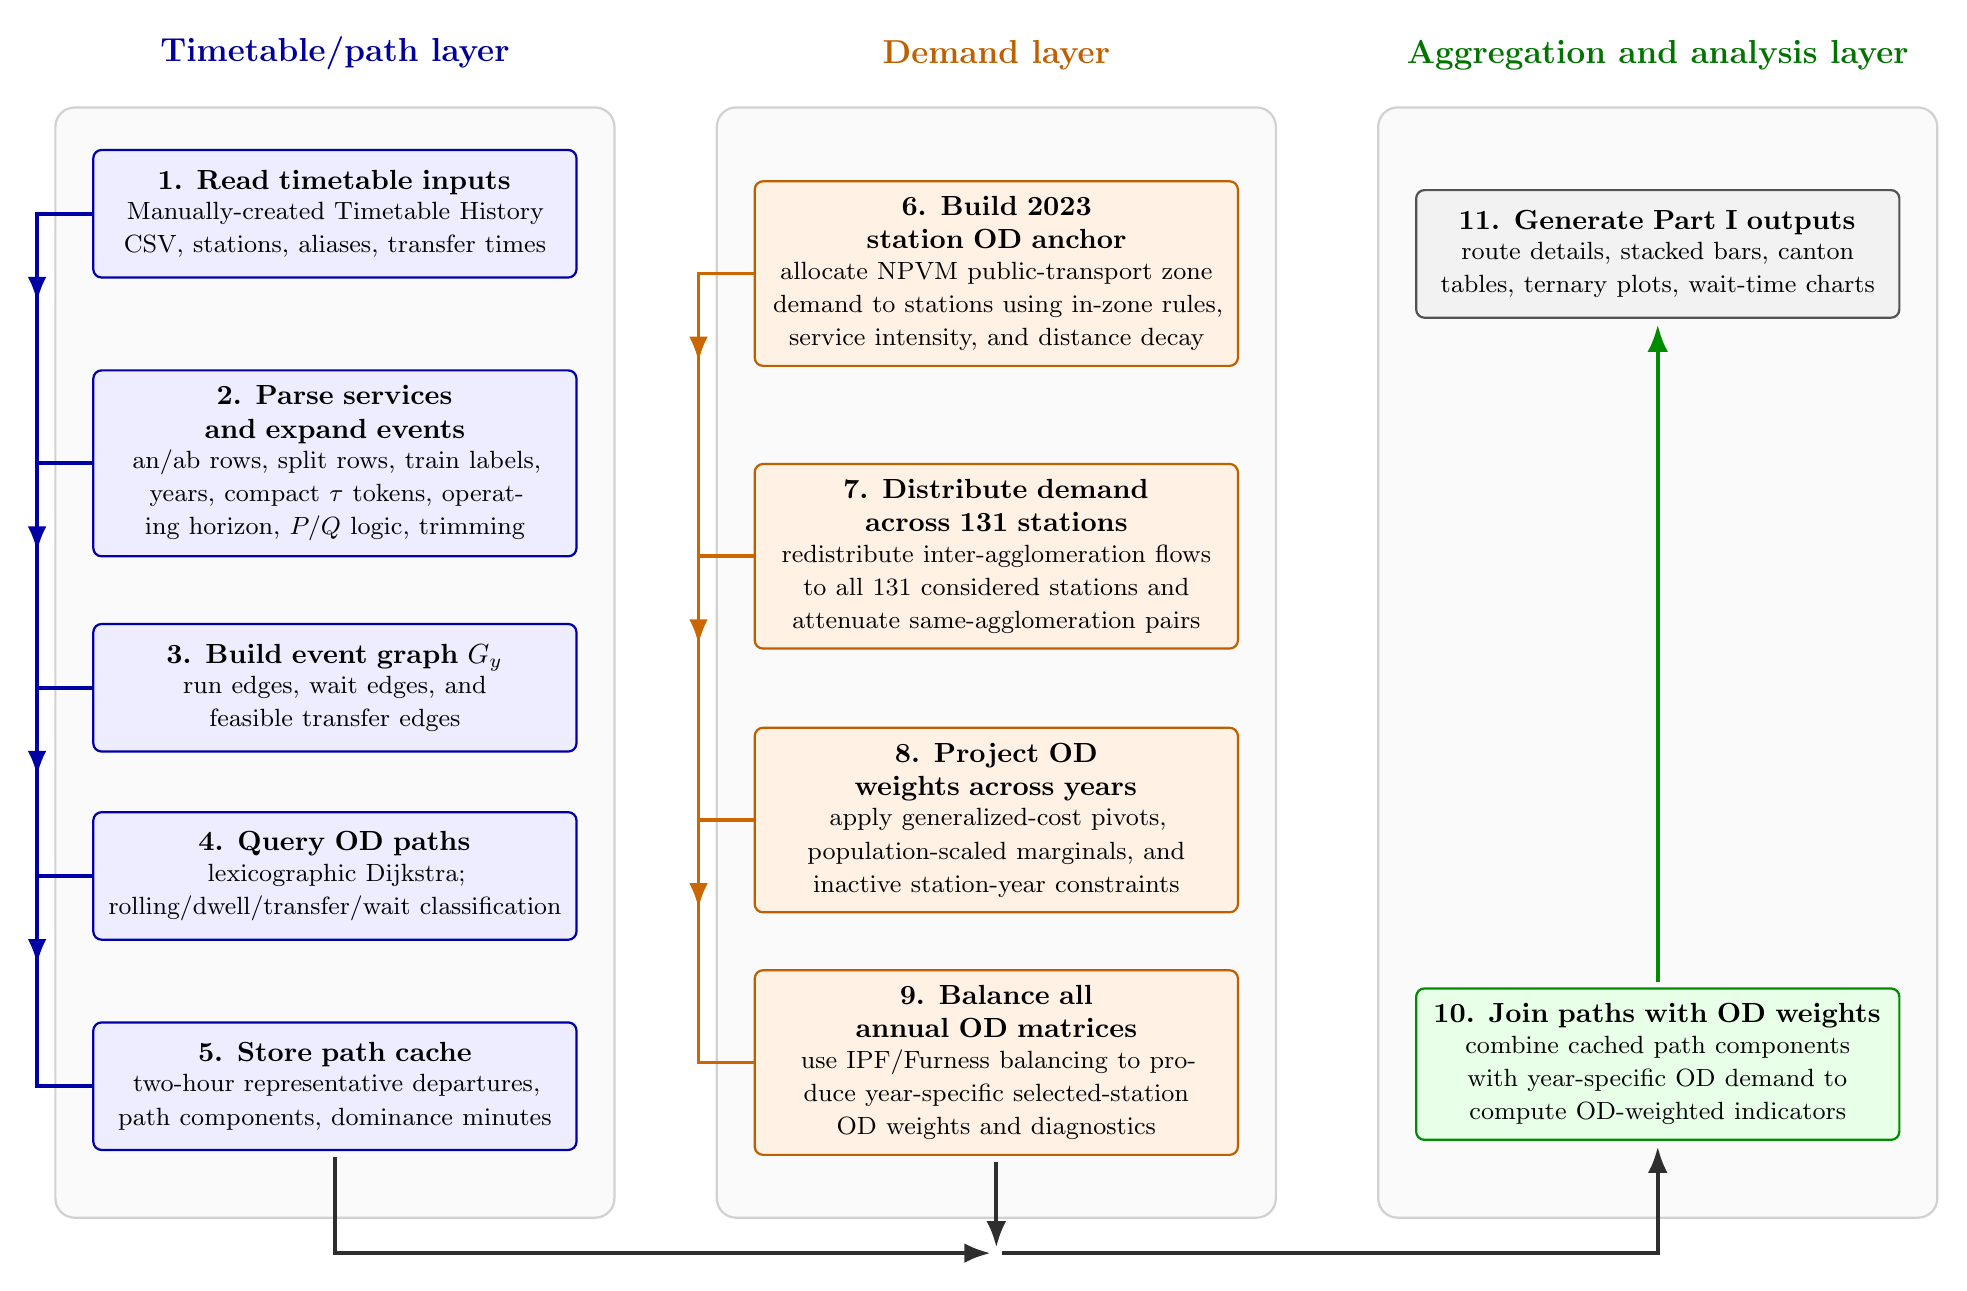
\begin{tikzpicture}[
    font=\normalsize,
    >=Latex,
    box/.style={
        rectangle,
        rounded corners=3pt,
        draw=black!55,
        line width=0.8pt,
        align=center,
        text width=5.75cm,
        minimum height=1.62cm,
        inner sep=5.5pt
    },
    pathbox/.style={
        box,
        fill=blue!7,
        draw=blue!65!black
    },
    demandbox/.style={
        box,
        fill=orange!10,
        draw=orange!75!black
    },
    appbox/.style={
        box,
        fill=green!9,
        draw=green!55!black
    },
    outputbox/.style={
        box,
        fill=gray!10,
        draw=gray!65!black
    },
    joinarrow/.style={
        ->,
        >=Latex,
        line width=1.45pt,
        draw=black!82,
        shorten >=2pt,
        shorten <=2pt
    },
    greenarrow/.style={
        ->,
        >=Latex,
        line width=1.55pt,
        draw=green!55!black,
        shorten >=2pt,
        shorten <=2pt
    },
    lane/.style={
        rounded corners=7pt,
        draw=black!18,
        line width=0.8pt,
        fill=black!2
    },
    lanetitle/.style={
        font=\large\bfseries,
        anchor=south
    }
]

% ---------------------------------------------------------------------
% Helper macros for side connectors with visible downward arrowheads
% ---------------------------------------------------------------------

\newcommand{\sideblue}[2]{%
    \draw[line width=1.35pt, draw=blue!65!black]
        (#1.west) -- ++(-0.70,0) |- (#2.west);
    \draw[->, >=Latex, line width=1.35pt, draw=blue!65!black]
        ($ (#1.west) + (-0.70,-0.78) $) -- ++(0,-0.34);
}

\newcommand{\sideorange}[2]{%
    \draw[line width=1.35pt, draw=orange!80!black]
        (#1.west) -- ++(-0.70,0) |- (#2.west);
    \draw[->, >=Latex, line width=1.35pt, draw=orange!80!black]
        ($ (#1.west) + (-0.70,-0.78) $) -- ++(0,-0.34);
}

% ---------------------------------------------------------------------
% Column and row coordinates
% ---------------------------------------------------------------------

\def\xT{0}
\def\xD{8.4}
\def\xA{16.8}

% Equal lane rectangles.
% laneTop is high enough that boxes 1, 6, and 11 sit fully inside.
% laneBottom is shortened to remove excess grey space below boxes 5, 9, and 10.
\def\laneTop{1.35}
\def\laneBottom{-12.75}
\def\laneHalfWidth{3.55}

% Timetable/path lane rows
\def\yOne{0}
\def\yTwo{-3.02}
\def\yThree{-5.89}
\def\yFour{-8.36}
\def\yFive{-11.08}

% Demand lane rows
\def\yDOne{-0.76}
\def\yDTwo{-4.35}
\def\yDThree{-7.7}
\def\yDFour{-10.78}

% Aggregation lane rows
% Step 11 is top-aligned with Steps 1 and 6.
\def\yAOutput{-0.51}
\def\yAJoin{-10.8}

% Shorter shared bottom join line
\def\yJoin{-13.20}

% ---------------------------------------------------------------------
% Lane backgrounds: identical grey rectangles
% ---------------------------------------------------------------------

\begin{pgfonlayer}{background}
    \draw[lane]
        (\xT-\laneHalfWidth,\laneTop)
        rectangle
        (\xT+\laneHalfWidth,\laneBottom);

    \draw[lane]
        (\xD-\laneHalfWidth,\laneTop)
        rectangle
        (\xD+\laneHalfWidth,\laneBottom);

    \draw[lane]
        (\xA-\laneHalfWidth,\laneTop)
        rectangle
        (\xA+\laneHalfWidth,\laneBottom);
\end{pgfonlayer}

% ---------------------------------------------------------------------
% Timetable/path layer: 1--5
% ---------------------------------------------------------------------

\node[pathbox] (t1) at (\xT,\yOne) {
    \textbf{1. Read timetable inputs}\\[-1pt]
    \small Manually-created Timetable History CSV, stations, aliases, transfer times
};

\node[pathbox] (t2) at (\xT,\yTwo-0.15) {
    \textbf{2. Parse services and expand events}\\[-1pt]
    \small an/ab rows, split rows, train labels, years, compact $\tau$ tokens, operating horizon, $P/Q$ logic, trimming
};

\node[pathbox] (t3) at (\xT,\yThree-0.13) {
    \textbf{3. Build event graph $G_y$}\\[-1pt]
    \small run edges, wait edges, and feasible transfer edges
};

\node[pathbox] (t4) at (\xT,\yFour-0.05) {
    \textbf{4. Query OD paths}\\[-1pt]
    \small lexicographic Dijkstra; rolling/dwell/transfer/wait classification
};

\node[pathbox] (t5) at (\xT,\yFive) {
    \textbf{5. Store path cache}\\[-1pt]
    \small two-hour representative departures, path components, dominance minutes
};

% ---------------------------------------------------------------------
% Demand layer: 6--9
% ---------------------------------------------------------------------

\node[demandbox] (d6) at (\xD,\yDOne) {
    \textbf{6. Build 2023 \\station OD anchor}\\[-1pt]
    \small allocate NPVM public-transport zone demand to stations using in-zone rules, service intensity, and distance decay
};

\node[demandbox] (d7) at (\xD,\yDTwo) {
    \textbf{7. Distribute demand across 131 stations}\\[-1pt]
    \small redistribute inter-agglomeration flows to all 131 considered stations and attenuate same-agglomeration pairs
};

\node[demandbox] (d8) at (\xD,\yDThree) {
    \textbf{8. Project OD weights across years}\\[-1pt]
    \small apply generalized-cost pivots, population-scaled marginals, and inactive station-year constraints
};

\node[demandbox] (d9) at (\xD,\yDFour) {
    \textbf{9. Balance all \\annual OD matrices}\\[-1pt]
    \small use IPF/Furness balancing to produce year-specific selected-station OD weights and diagnostics
};

% ---------------------------------------------------------------------
% Aggregation and analysis layer: 10--11, inverted
% ---------------------------------------------------------------------

\node[outputbox] (a11) at (\xA,\yAOutput) {
    \textbf{11. Generate Part I outputs}\\[-1pt]
    \small route details, stacked bars, canton tables, ternary plots, wait-time charts
};

\node[appbox] (a10) at (\xA,\yAJoin) {
    \textbf{10. Join paths with OD weights}\\[-1pt]
    \small combine cached path components with year-specific OD demand to compute OD-weighted indicators
};

% ---------------------------------------------------------------------
% Lane titles
% ---------------------------------------------------------------------

\node[lanetitle, text=blue!60!black] at (\xT,\laneTop+0.35)
{Timetable/path layer};

\node[lanetitle, text=orange!75!black] at (\xD,\laneTop+0.35)
{Demand layer};

\node[lanetitle, text=green!45!black] at (\xA,\laneTop+0.35)
{Aggregation and analysis layer};

% ---------------------------------------------------------------------
% Internal lane arrows: side links with visible downward arrowheads
% ---------------------------------------------------------------------

% Timetable/path lane
\sideblue{t1}{t2}
\sideblue{t2}{t3}
\sideblue{t3}{t4}
\sideblue{t4}{t5}

% Demand lane
\sideorange{d6}{d7}
\sideorange{d7}{d8}
\sideorange{d8}{d9}

% Aggregation lane: straight green 10 -> 11
\draw[greenarrow] (a10.north) -- (a11.south);

% ---------------------------------------------------------------------
% Seamless bottom join:
% Step 5 and Step 9 merge at the bottom, then continue together to Step 10.
% ---------------------------------------------------------------------

% Step 5 drops to the shared bottom route.
\draw[joinarrow]
    (t5.south)
    -- ++(0,-0.35)
    -- (\xT,\yJoin)
    -- (\xD,\yJoin);

% Step 9 drops into the same route at the merge point.
\draw[joinarrow]
    (d9.south)
    -- ++(0,-0.35)
    -- (\xD,\yJoin);

% Shared continuation into Step 10.
\draw[joinarrow]
    (\xD,\yJoin)
    -- (\xA,\yJoin)
    -- (a10.south);

\end{tikzpicture}%
}
\caption[Part I modelling workflow]{Part I modelling workflow. The timetable/path layer reads the historical timetable inputs, parses compact timetable tokens into concrete events, builds year-specific event graphs, queries OD paths, and stores two-hour dominance-weighted path-component caches. The demand layer converts NPVM 2023 public-transport zone demand into a station-level OD anchor, derives the 131-station analysis layer, projects OD weights across historical timetable years using generalized-cost pivots and population-scaled marginals, and balances annual OD matrices with IPF. The aggregation layer joins the prepared path-component cache with year-specific OD weights to produce OD-weighted historical indicators and analysis outputs.}

\label{fig:part1-workflow}
\end{figure}

\begin{figure}[htbp]
\centering
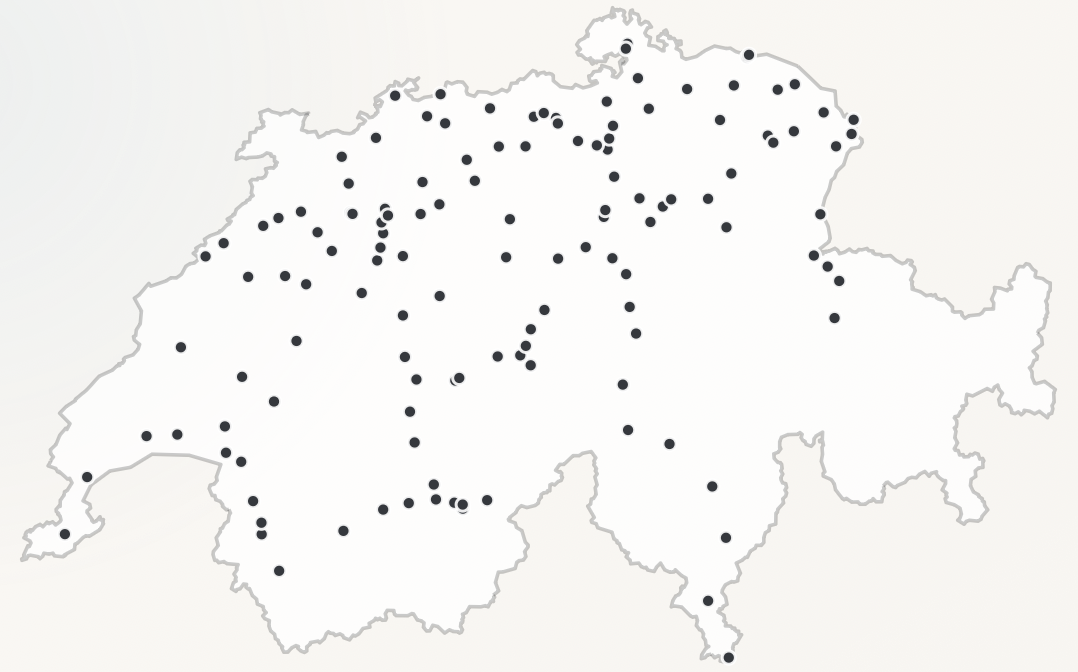
\includegraphics[width=0.6\textwidth]{figures/131 stations.png}
\caption[Part I station map]{Locations of the 131 stations considered in Part I, connected by 65 line services}

\label{fig:131_stations}
\end{figure}


\subsection{Timetable/path layer}



The following chapters describe the timetable/path layer of Figure~\ref{fig:part1-workflow}: compact timetable entries are converted into event graphs, OD paths are queried, and the resulting path components are stored in a two-hour dominance cache for later combination with the demand layer. 

\subsubsection{Periodic timetable expansion and route graph}\label{sec:methods-part1-eventgraph}
The compact timetable tokens are expanded into concrete event times. Let $H(\tau_k)$ be the allowed hour set for token $\tau_k$:
\begin{equation}
H(\tau_k)=
\begin{cases}
\{5,6,\ldots,26\}, & \mu_k=\mathrm{hourly},\\
\{h\in\{5,\ldots,26\}: h\bmod 2=0\}, & \mu_k=\mathrm{even},\\
\{h\in\{5,\ldots,26\}: h\bmod 2=1\}, & \mu_k=\mathrm{odd}.
\end{cases}
\label{eq:allowed-hours}
\end{equation}
Here, $h$ [h] is a clock-hour index and $\mu_k$ [categorical] is the frequency mode analogous to the suffixless, $i$, and $n$ suffixes added to the clock-hour in the examples in Chapter \ref{sec:logic}. Departure events are retained for $300\le t<1440$ [min], i.e. between 05:00 and 23:59.

For a train-run chain of events along a line, the next concrete event is
\begin{equation}
  t_k=\min\{60h+m_k: h\in H(\tau_k),\ 60h+m_k\ge b_k\},
  \label{eq:next-event-time}
\end{equation}

where $t_k$ [min] is the selected event time, $m_k$ [min] is the minute-of-hour token, and $b_k$ [min] is the lower bound implied by the previous event. The lower bound is

\begin{equation}
  b_k =
  \begin{cases}
    t_{k-1}, & P_k=0 \text{ and } Q_k=0, \\[6pt]
    t_{k-1}+60, & P_k=1 \text{ or } Q_k=1.
  \end{cases}
  \label{eq:continuation-bound}
\end{equation}
where $t_{k-1}$ [min] is the time of the previous event in the same train-run chain. The Boolean flags $P_k$ and $Q_k$ are ignored when absent. $P_k$ is used for two-hourly lines and $Q_k$ for hourly lines, but both have the effect of pushing the following event at least a full hour after the preceding event; see examples in Chapter~\ref{sec:logic}.

Once all line service chains for a given timetable year have been expanded in this way, all the resulting arrival and departure events are assembled into a directed time-expanded event graph. For each year $y$, the expanded timetable is represented as

\begin{equation}
  G^y=(V^y,E^y_{\mathrm{run}}\cup E^y_{\mathrm{wait}}\cup E^y_{\mathrm{transfer}}),
  \label{eq:historical-event-graph}
\end{equation}

where $G^y$ is the graph for timetable year $y$, $V^y$ is the set of event nodes, and $E^y_{\mathrm{run}}$, $E^y_{\mathrm{wait}}$, and $E^y_{\mathrm{transfer}}$ are three sets of directed edges. The event nodes $V^y$ store station, event kind, exact minute, service label, segment index, and trip instance.

The three edge sets encode the feasible passenger actions available from each event node. Run edges connect consecutive events on the same concrete train run, such as a departure from one station to the next arrival. Wait edges connect later departure events at the same station in chronological order, allowing the search to remain at a station until a later service becomes available. Transfer edges connect arrival events to feasible departures of different train services after the station-specific minimum transfer time has been satisfied.

After the graph setup, a route search can then be performed within the event graph of each timetable year. For a query from origin $o$ to destination $d$ with query time $q$, the search is seeded at the origin station at minute $q$ and may use all temporally reachable events in $G^y$ after that minute. The distinction between run, wait, and transfer edges is used to construct and later classify paths, but the route search itself processes them within the same graph traversal. When the shortest-path Dijkstra algorithm reaches an event node, it evaluates the outgoing edges available from that node regardless of edge type. The station, time, event kind, and train identity stored in the node determine which outgoing actions exist. For transfer actions, departures at each station are ordered by time; after an arrival event, the applicable station-specific minimum transfer time is added, and the corresponding station departure list is used to identify the next feasible departure of a different train service. This keeps intermediate transfers inside the same Dijkstra search.

The described shortest-path search assigns each reached event node $v$ a lexicographic route label as follows:
\begin{equation}
  c(v)=\left(a_v,-f_v,x_v,n_v\right),
  \label{eq:lexicographic-label}
\end{equation}
which summarizes the best known nondominated route to that node. The labels are compared lexicographically, so the first component has highest priority, followed by the second, third, and fourth components only in the case of ties. Here, $a_v$ [min] is the event time reached and is minimized first. Among routes with the same arrival time, $-f_v$ is minimized, which is equivalent to maximizing the first boarded departure time $f_v$ [min]. This favours the latest possible departure among equally early arrivals and avoids selecting journeys that start unnecessarily early. If both arrival time and first departure time are equal, the number of transfers $x_v$ [count] is minimized. Finally, if these criteria are still tied, the number of movement segments $n_v$ [count] is minimized, i.e. express trains are prioritized over trains that stop more frequently.

\subsubsection{Two-hour dominance cache and timetable components}\label{sec:methods-part1-cache}

The route graph described above can return a path for a specific origin, destination, timetable year, and passenger query time. However, the historical analysis requires a representative timetable measure for each origin--destination pair and year, rather than a result for only one departure minute. To obtain this, the model queries each origin--destination--year combination repeatedly over a representative two-hour clockface cycle. Let $o$ denote the origin station, $d$ the destination station, and $y$ the timetable year. The set of passenger query departure times is
\begin{equation}
  Q=\{300,301,\ldots,419\},
  \label{eq:query-minute-set}
\end{equation}
where each $q\in Q$ is a passenger query time in minutes after midnight. This corresponds to one query per minute from 05:00 to 06:59. The two-hour span is used because the historical timetable is represented as a repeating two-hour clockface pattern. Sampling every query minute within this cycle assigns each retained path a dominance interval while keeping the all-year cache computationally manageable. For each query minute $q$, the route search returns the best nondominated path from $o$ to $d$ in year $y$ according to the lexicographic ranking in Equation~\eqref{eq:lexicographic-label}. All resulting query-level paths with departure times within the initial two-hour period are collected, and will be repeated throughout the day until the destination is no longer reachable. Each distinct grouped alternative is denoted by $\pi$. Let $\Pi^y_{od}$ be the set of retained path alternatives for origin--destination pair $(o,d)$ in year $y$. Each grouped path $\pi\in\Pi^y_{od}$ receives a dominance-minute count
\begin{equation}
  \beta^y_{od\pi}=\left|\{q\in Q: \pi \text{ is selected for } (o,d,y) \text{ at query minute } q\}\right|,
  \label{eq:part1-dominance-minutes}
\end{equation}
where $\beta^y_{od\pi}$ [min] is the number of queried minutes in the two-hour cycle for which path alternative $\pi$ is selected. This can be interpreted as a random-arrival exposure approximation: a path selected over 30 queried departure minutes receives twice the weight of a path selected over 15 queried minutes. Figure~\ref{fig:dominance-cache-example} illustrates this logic for a simplified two-station service between stations A and B. Five nondominated departures are retained within the representative two-hour cycle: 05:03, 05:33, 05:48, 06:03, and 06:33. Since the clockface cycle repeats, query minutes after 06:33 are assigned to the next occurrence of the 05:03-pattern departure. The dominance-minute weights are therefore 30, 30, 15, 15, and 30 minutes, respectively. With travel times of 20 minutes for departures ending in :03, 18 minutes for departures ending in :33, and 25 minutes for the :48 departure, the representative dominance-weighted in-vehicle travel time in this example is
\begin{equation}
  \bar\theta =
  \frac{30\cdot20+30\cdot18+15\cdot25+15\cdot20+30\cdot18}
  {30+30+15+15+30}
  =19.63\text{ min}.
  \label{eq:dominance-example-weighted-time}
\end{equation}

\begin{figure}[htbp]
\centering
\resizebox{\textwidth}{!}{%
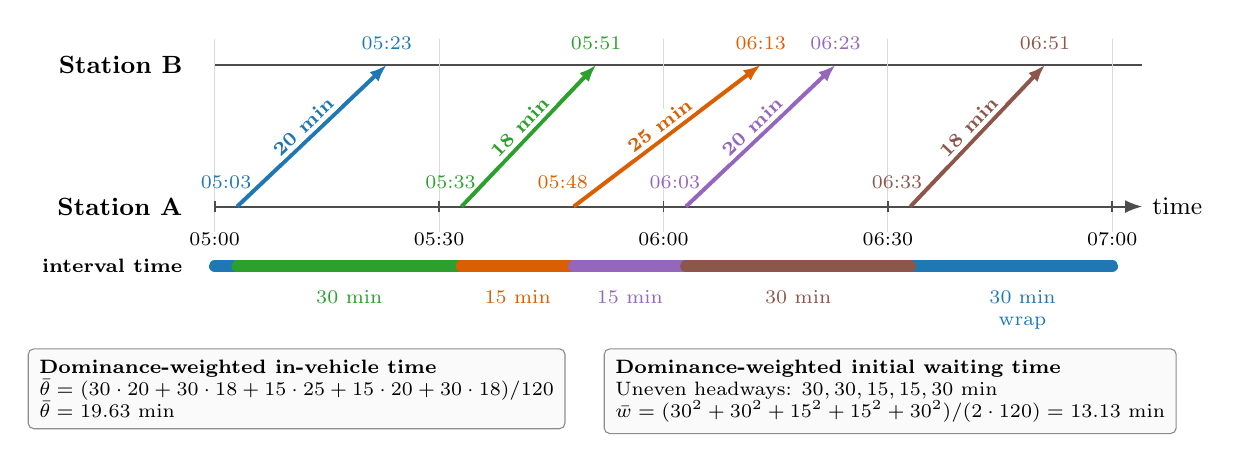
\begin{tikzpicture}[
    x=0.095cm,
    y=1.8cm,
    font=\small,
    >=Latex,
    train/.style={line width=1.45pt, -{Latex[length=2.2mm]}},
    exposure/.style={line width=4.2pt, line cap=round},
    axis/.style={line width=0.7pt, draw=black!70},
    gridline/.style={draw=black!15, line width=0.4pt},
    timelabel/.style={font=\scriptsize, align=center},
    stationlabel/.style={font=\small\bfseries, anchor=east},
    routeLabel/.style={font=\scriptsize\bfseries, fill=white, inner sep=1.5pt},
    box/.style={draw=black!45, fill=black!2, rounded corners=2pt, inner sep=4pt, font=\scriptsize, align=left}
]

% Time coordinate:
% x = minutes after 05:00.
% Station A is y=0, station B is y=1.

\definecolor{depA}{HTML}{1F77B4}
\definecolor{depB}{HTML}{2CA02C}
\definecolor{depC}{HTML}{D95F02}
\definecolor{depD}{HTML}{9467BD}
\definecolor{depE}{HTML}{8C564B}

% Axes
\draw[axis, ->] (0,0) -- (124,0) node[anchor=west, font=\small] {time};
\draw[axis] (0,1) -- (124,1);
\node[stationlabel] at (-3,0) {Station A};
\node[stationlabel] at (-3,1) {Station B};

% Hour markers and grid
\foreach \x/\lab in {0/05:00,30/05:30,60/06:00,90/06:30,120/07:00}{
    \draw[gridline] (\x,-0.18) -- (\x,1.18);
    \draw[axis] (\x,0.04) -- (\x,-0.04);
    \node[timelabel, anchor=north] at (\x,-0.12) {\lab};
}

% Train lines: departure x, arrival x+travel time
\draw[train, depA] (3,0) -- (23,1)
    node[midway, sloped, above, routeLabel, text=depA] {20 min};
\node[timelabel, text=depA, anchor=south east] at (6.2,0.06) {05:03};
\node[timelabel, text=depA, anchor=south] at (23,1.04) {05:23};

\draw[train, depB] (33,0) -- (51,1)
    node[midway, sloped, above, routeLabel, text=depB] {18 min};
\node[timelabel, text=depB, anchor=south east] at (36.2,0.06) {05:33};
\node[timelabel, text=depB, anchor=south] at (51,1.04) {05:51};

\draw[train, depC] (48,0) -- (73,1)
    node[midway, sloped, above, routeLabel, text=depC] {25 min};
\node[timelabel, text=depC, anchor=south east] at (51.2,0.06) {05:48};
\node[timelabel, text=depC, anchor=south] at (73,1.04) {06:13};

\draw[train, depD] (63,0) -- (83,1)
    node[midway, sloped, above, routeLabel, text=depD] {20 min};
\node[timelabel, text=depD, anchor=south east] at (66.2,0.06) {06:03};
\node[timelabel, text=depD, anchor=south] at (83,1.04) {06:23};

\draw[train, depE] (93,0) -- (111,1)
    node[midway, sloped, above, routeLabel, text=depE] {18 min};
\node[timelabel, text=depE, anchor=south east] at (95.9,0.06) {06:33};
\node[timelabel, text=depE, anchor=south] at (111,1.04) {06:51};

% Interval window bar below Station A
\def\yexp{-0.42}
\node[font=\scriptsize\bfseries, anchor=east] at (-3,\yexp) {interval time};

% Exposure intervals:
% 05:03-pattern departure: 05:00-05:03 plus wrap 06:33-07:00 = 30 min
\draw[exposure, depA] (0,\yexp) -- (3,\yexp);
\draw[exposure, depA] (93,\yexp) -- (120,\yexp);
\node[timelabel, text=depA, anchor=north] at (108,\yexp-0.10) {30 min\\wrap};

% 05:33 departure: 05:03-05:33 = 30 min
\draw[exposure, depB] (3,\yexp) -- (33,\yexp);
\node[timelabel, text=depB, anchor=north] at (18,\yexp-0.10) {30 min};

% 05:48 departure: 05:33-05:48 = 15 min
\draw[exposure, depC] (33,\yexp) -- (48,\yexp);
\node[timelabel, text=depC, anchor=north] at (40.5,\yexp-0.10) {15 min};

% 06:03 departure: 05:48-06:03 = 15 min
\draw[exposure, depD] (48,\yexp) -- (63,\yexp);
\node[timelabel, text=depD, anchor=north] at (55.5,\yexp-0.10) {15 min};

% 06:33 departure: 06:03-06:33 = 30 min
\draw[exposure, depE] (63,\yexp) -- (93,\yexp);
\node[timelabel, text=depE, anchor=north] at (78,\yexp-0.10) {30 min};

% Calculation box
\node[box, anchor=north west] at (-25,-1.0) {
\textbf{Dominance-weighted in-vehicle time}\\
$\bar\theta=(30\cdot20+30\cdot18+15\cdot25+15\cdot20+30\cdot18)/120$\\
$\bar\theta=19.63$ min
};

\node[box, anchor=north west] at (52,-1.0) {
\textbf{Dominance-weighted initial waiting time}\\
Uneven headways: $30,30,15,15,30$ min\\
$\bar w=(30^2+30^2+15^2+15^2+30^2)/(2\cdot120)=13.13$ min
};

\end{tikzpicture}%
}

\caption[Dominance-minute calculation]{Illustrative dominance-minute calculation for a two-station clockface service between stations A and B over a repeating two-hour interval. Diagonal lines show train movements and their in-vehicle travel times. The interval bar shows the departure window before each departure.}

\label{fig:dominance-cache-example}
\end{figure}

For any path-level time component $\theta_\pi$ [min], such as rolling time, dwell time, transfer time, or total post-departure time, the OD-level cache stores the dominance-weighted average
\begin{equation}
  \bar\theta^y_{od}=\frac{\sum_{\pi\in\Pi^y_{od}} \beta^y_{od\pi}\theta_\pi}
  {\sum_{\pi\in\Pi^y_{od}} \beta^y_{od\pi}}.
  \label{eq:dominance-weighted-od-metric}
\end{equation}
Here, $\bar\theta^y_{od}$ [min] is the representative value of time component $\theta$ for OD pair $(o,d)$ in year $y$. The numerator sums the component value of each retained path alternative weighted by the number of queried minutes for which that path is selected, while the denominator normalizes by the total number of reachable selected minutes. 
Initial waiting time describes the time before the passenger boards the first train, and is described as follows. Let $Q^*_{od}\subseteq Q$ be the subset of queried minutes for which a route from $o$ to $d$ is reachable, and let $f_q$ [min] be the first boardable nondominated departure time returned by the route query launched at query minute $q$. The average initial waiting time is therefore
\begin{equation}
  \bar w^y_{od}=\frac{1}{|Q^*_{od}|}\sum_{q\in Q^*_{od}}\max(f_q-q,0),
  \label{eq:part1-initial-wait}
\end{equation}
where $\bar w^y_{od}$ [min] is the representative pre-boarding waiting time for OD pair $(o,d)$ in year $y$. In Figure~\ref{fig:dominance-cache-example}'s example, the corresponding headways are 2x 15 min and 3x 30 min, giving
\begin{equation}
  \bar w =
  \frac{30^2+30^2+15^2+15^2+30^2}{2\cdot120}
  =13.13\text{ min}.
  \label{eq:dominance-example-waiting-time}
\end{equation}
This differs from a simple frequency-based approximation. If the five trains were treated as evenly distributed across two hours, the average headway would be $120/5=24$ minutes and the implied average waiting time would be $24/2=12$ minutes. The dominance-cache calculation instead takes into account the actual uneven spacing of departures. This pre-departure waiting time is reported independently from the defined total time, which describes only post-departure travel and consists of rolling, dwell, and transfer time.

\subsection{Demand layer}\label{sec:demand}

The next step is to construct the corresponding demand layer. This layer starts from the NPVM public-transport zone matrix, converts zone-level flows into station-level OD weights, reduces the result to the 131-station analysis layer, and then projects the accepted 2023 demand anchor across historical timetable years.

\subsubsection{Station allocation from NPVM zones}\label{sec:methods-part1-npvm}

The 2023 demand anchor is derived from the NPVM 2023 public-transport zone-to-zone matrix \citep{vmuvek2026npvm2023}. The NPVM matrix itself is zone-based rather than station-based. Let $Z$ be the set of NPVM traffic zones; this set contains 8,688 zones. Let $S_{250}$ denote the broader set of 250 target stations that appear in at least one of the considered timetable years. The first demand-layer step converts each NPVM zone into fractional station shares over $S_{250}$ and applies these shares to the official public-transport OD matrix. This 250 station layer is used before the reduction to the 131-station layer so that the zone-to-station allocation can use all stations that are relevant in at least one timetable year. The subsequent 131-station layer is then derived for the historical indicators, where comparability across years is required.

The allocation is performed from the perspective of each NPVM zone, not from the perspective of a station. For each zone $z\in Z$, the model constructs a candidate station set $C_z\subseteq S_{250}$. This set first includes all target stations whose point geometry lies inside the zone polygon. The model then computes the distance from the zone centroid to every station in $S_{250}$ and adds nearby stations in order of centroid distance. The implemented parameters are a minimum of four stations and a nearest-station pool of six candidate stations. In practice, this means that a zone with no target station inside its polygon is represented by nearby stations around its centroid, with at least four candidates retained and normally up to the six nearest stations considered. A zone with one, two, or three in-zone stations is supplemented with nearby stations until the minimum candidate count is reached, while the six-station pool keeps additional nearby alternatives available for the allocation. If more than six target stations lie inside a zone, all in-zone stations are retained rather than being truncated to six. The allocation is therefore normalized only within the zone-specific candidate station set $C_z$, not across all stations in the network.

For each candidate station $s\in C_z$, the implemented raw allocation score is
\begin{equation}
 a^{\mathrm{raw}}_{zs}
  =
  B_{zs}
  \frac{\sqrt{L_s/(1\ \mathrm{line/day})}}
  {\left(d_{zs}/(1\ \mathrm{km})+3\right)^{2}},
  \label{eq:zone-station-raw-weight}
\end{equation}
where $a^{\mathrm{raw}}_{zs}$ is the raw allocation score, $L_s$ is a count of the number of line services per day in 2023  calling at station $s$, and $d_{zs}$ [km] is the distance between the centroid of zone $z$ and station $s$. The factor $B_{zs}$ is a heuristically chosen in-zone bonus of 1.75 if the station lines inside the zone, and 1 otherwise. This factor only affects the relative allocation among the stations in $C_z$. For example, if a zone has one in-zone station and five nearby outside-zone stations, the in-zone station receives the multiplier 1.75 compared to the other five. If a zone has no in-zone station, all surrounding candidates have $B_{zs}=1$ and the allocation is determined only by service intensity and distance from the zone centroid. The square-root line service term rewards better-served stations without allowing major hubs to absorb all demand, while the distance-decay term favours stations closer to the zone centroid. The experimentally-chosen 3 km offset dampens the distance term so that extremely small centroid-to-station distances do not dominate the allocation. The scores are normalized within each zone as follows:
\begin{equation}
  A_{zs}=\frac{a^{\mathrm{raw}}_{zs}}{\sum_{k\in C_z}a^{\mathrm{raw}}_{zk}},
  \label{eq:zone-station-share}
\end{equation}
where $A_{zs}$ is the share of zone $z$ assigned to candidate station $s$. By design, the station shares of each zone sum to 1 across its candidate set $C_z$. The station OD matrix is then obtained by fractionally distributing each NPVM zone-to-zone flow $F_{ab}$ [pax/day] over the station candidates of its origin and destination zones:
\begin{equation}
  T^{\mathrm{station}}_{ij}=\sum_{a,b\in Z} F_{ab} A_{ai}A_{bj}.
  \label{eq:station-od-anchor}
\end{equation}
Here, $T^{\mathrm{station}}_{ij}$ [pax/day] is the directed station-to-station demand assigned from the NPVM matrix. For each zone pair $(a,b)$, the product $A_{ai}A_{bj}$ distributes the zone-level flow to OD station pair $(i,j)$ according to the origin-zone and destination-zone station shares. This creates a 2023 demand network at a station level, which is used as an anchor to later recalculate the other years from. The OD demand core comes from the official NPVM matrix, while the conversion from zones to stations is performed through the above documented hybrid distance--service allocation rules. In total, 8'688 zones, 250 modelled and 131 filtered stations, 17'026'407 matrix rows, and 2'951'903 allocated station trips are considered.

\subsubsection{Same-agglomeration attenuation}\label{sec:methods-part1-agglomeration}
The 131-station analysis layer required special treatment of dense urban areas. Without correction, the station-level OD allocation was found to overstate short same-agglomeration pairs because several stations inside one urban region are also typically served by other modes, such as local buses or trams. The introduced attenuation rule keeps same-agglomeration pairs but scales them by distance:
\begin{equation}
    W^{2023}_{ij}
  =
  T^{\mathrm{raw}}_{ij}
  \min\left(1,\frac{d_{ij}}{60\ \mathrm{km}}\right),
  \label{eq:same-agglomeration-attenuation}
\end{equation}
for same-agglomeration selected-station pairs. Here, $W^{2023}_{ij}$ [pax/day] is the accepted 2023 selected-layer pair weight, $T^{\mathrm{raw}}_{ij}$ [pax/day] is the raw selected-station demand, and $d_{ij}$ [km] is station crow-fly distance. Inter-agglomeration selected-station pairs retain $W^{2023}_{ij}=T^{\mathrm{raw}}_{ij}$. The 60 km denominator is a calibrated attenuation scale: it strongly damps very short intra-urban station pairs that were overrepresented by zone allocation, but returns to full weight for longer regional pairs, making for a more realistic portrayal of rail usage.

\subsubsection{Historical generalized-cost projection}\label{sec:methods-part1-gc}

The accepted 2023 selected-station matrix $W^{2023}_{ij}$ serves as the demand anchor in Part I. The purpose of this section is to project the 2023 OD pattern across other timetable years. The projection is based on a simple idea: if travel between a given OD pair is faster in year $y$ than in 2023, its provisional demand weight is increased; if it is slower, its provisional demand weight is reduced. This produces a year-specific seed matrix, which is then balanced to year-specific origin and destination totals in the IPF step in Section~\ref{sec:methods-part1-ipf}.

For each OD pair $(i,j)$ and timetable year $y$, the model first computes a representative elapsed travel time from the timetable route search. Let $\mathcal{H}$ denote the representative query-time set used for this calculation (early-morning departures during a two-hour time period), and let $e^y_{ijh}$ [min] be the elapsed time from query time $h\in\mathcal{H}$ to arrival. Since all retained OD-year pairs are reachable for all representative query times, the generalized cost is defined as the mean elapsed time:

\begin{equation}
GC^y_{ij}=
\frac{1}{|\mathcal{H}|}
\sum_{h\in \mathcal{H}} e^y_{ijh}.
\label{eq:historical-generalized-cost}
\end{equation}

Here, $GC^y_{ij}$ [min] is the representative timetable-based elapsed-time value the OD pair $(i,j)$ in year $y$. It is the average elapsed time returned by the route queries at the query times in $h\in\mathcal{H}$. This value is used to compare each historical timetable year with the 2023 demand anchor. The generalized-cost sensitivity is calibrated using the accepted 2023 OD rows. The calibration does not attempt to explain total station-to-station demand from travel time alone, but instead first removes the 2023 OD demand pattern. The independence expectation is

\begin{equation}
  I_{ij}=\frac{O^{2023}_iD^{2023}_j}{\sum_{a,b}W^{2023}_{ab}},
  \qquad
  z_{ij}=\log\left(\frac{W^{2023}_{ij}}{I_{ij}}\right),
  \label{eq:independence-residual}
\end{equation}

where $O^{2023}_i$ and $D^{2023}_j$ [pax/day] are the 2023 origin and destination totals, $I_{ij}$ [pax/day] is the OD weight expected if origins and destinations combined independently, and $z_{ij}$ [unitless] is the log deviation of the accepted 2023 OD weight from this expectation.

The relationship between this deviation and the timetable-based elapsed-time value is then estimated as
\begin{equation}
  z_{ij}
  =
  \alpha
  -
  \beta\log\left(\frac{GC^{2023}_{ij}}{1\ \mathrm{min}}\right)
  +
  \varepsilon_{ij}.
  \label{eq:gc-beta-calibration}
\end{equation}
The parameter $\alpha$ is the fitted intercept, $\beta$ is the generalized-cost sensitivity, $GC^{2023}_{ij}$ [min] is the 2023 generalized cost, and $\varepsilon_{ij}$ is the residual. The negative sign before $\beta$ means that OD pairs with higher elapsed-time values tend to have lower demand than would be expected from their origin and destination totals alone. The implemented weighted regression uses $\sqrt{W^{2023}_{ij}}$ as the row weight, so larger observed OD flows have more influence on the fit without letting the largest flows dominate linearly. The fitted values are $\beta=1.777396$ and $\alpha=7.763374$, using 17,030 active OD rows, with a weighted $R^2$ of 0.44006. This $R^2$ describes the fit to the log deviation from the independence expectation, which focuses on the part of the OD pattern associated with timetable-based elapsed time.

The calibrated sensitivity is then used to pivot the 2023 OD weight to each timetable year:
\begin{equation}
  S^y_{ij}=W^{2023}_{ij}\left(\frac{GC^{2023}_{ij}}{GC^y_{ij}}\right)^{\beta},
  \label{eq:historical-pivot-seed}
\end{equation}
where $S^y_{ij}$ [pax/day] is the pre-balancing OD weight for station pair $(i,j)$ in year $y$. It is obtained by applying the calibrated generalized-cost response to the accepted 2023 OD weight. The term $\left(GC^{2023}_{ij}/GC^y_{ij}\right)^{\beta}$ is defined as the generalized-cost multiplier. If travel between $i$ and $j$ is faster in year $y$ than in 2023, then $GC^y_{ij}<GC^{2023}_{ij}$ and this multiplier is greater than one, so the pre-balancing OD weight increases. If travel is slower than in 2023, the multiplier is below one and the pre-balancing OD weight decreases. The resulting matrix $S^y$ is passed to the IPF step, where it is adjusted to match the year-specific origin and destination totals.



\subsubsection{IPF balancing}\label{sec:methods-part1-ipf}

The generalized-cost pivot in Equation~\eqref{eq:historical-pivot-seed} produces a year-specific seed matrix $S^y$, but this seed does not yet enforce plausible station-level totals for year $y$. The final demand-layer step therefore balances $S^y$ to year-specific production and attraction targets using iterative proportional fitting (IPF), also known as Furness balancing.

The station-year population figures were sourced from BFS municipality population counts, GeoAdmin municipality assignment, and canton-level BFS population growth factors \citep{swisstopoGeoAdminIdentify, bfsCantonPopulation2024, bfsMunicipalityPopulation2024, bfsCantonPopulationScenarios2025}. Observed canton totals are used for past years, while 2025, 2026, and 2035 use the BFS reference population scenario. The 2023 OD anchor itself is based on NPVM 2023 \citep{vmuvek2026npvm2023}.

For each station in Switzerland, the base value is the station municipality's 2023 BFS population. This base is scaled to each timetable year using the corresponding cantonal growth factor relative to 2023.  Where several modelled stations share the same municipality base, the municipality population is split between them according to the station's year-specific service count, which makes the simplified assumption that stations with more departures (e.g. Zürich HB) will have proportionally more demand than stations with fewer departures in the same municipality (e.g. Zürich Wipkingen). For each origin station $o$ and destination station $d$, the raw year-specific production and attraction targets are

\begin{equation}
  \widetilde O^y_o
  =
  \epsilon^y_o O^{2023}_o
  \frac{Pop^y_o}{Pop^{2023}_o},
  \qquad
  \widetilde D^y_d
  =
  \epsilon^y_d D^{2023}_d
  \frac{Pop^y_d}{Pop^{2023}_d}.
  \label{eq:historical-raw-population-marginals}
\end{equation}
Here, $\widetilde O^y_o$ and $\widetilde D^y_d$ [pax/day] are the raw population-scaled production and attraction targets before total adjustment. $O^{2023}_o$ and $D^{2023}_d$ [pax/day] are the accepted 2023 origin and destination station flow totals, and $Pop^y_o$ and $Pop^y_d$ [persons] are the station-year population figures. The Boolean variable $\epsilon^y_i$ is 1 only if the station is active in year $y$ and has positive service in the filtered station file, otherwise it is 0. Inactive station-years are set to zero on both the origin and destination sides. Because production and attraction totals are scaled independently, their raw sums can differ slightly. Both sides are therefore rescaled to a common yearly total:

\begin{equation}
  T^y
  =
  \frac{1}{2}
  \left(
    \sum_o \widetilde O^y_o
    +
    \sum_d \widetilde D^y_d
  \right),
  \label{eq:historical-common-total}
\end{equation}

with the final marginal targets defined as

\begin{equation}
  O^y_o
  =
  \widetilde O^y_o
  \frac{T^y}{\sum_{o'} \widetilde O^y_{o'}},
  \qquad
  D^y_d
  =
  \widetilde D^y_d
  \frac{T^y}{\sum_{d'} \widetilde D^y_{d'}}.
  \label{eq:historical-rescaled-marginals}
\end{equation}

Here, $T^y$ [pax/day] is the common flow total used for the year-$y$ matrix, while $O^y_o$ and $D^y_d$ [pax/day] are the compatible production and attraction targets passed to IPF.

Starting from the pre-balancing matrix $S^y$, IPF alternates row and column scaling. The initial matrix is

\[
  M^{y,(0)}_{od}=S^y_{od}.
\]

At each iteration, the row-scaling step adjusts each origin total to its target $O^y_o$, and the column-scaling step adjusts each destination total to its target $D^y_d$:

\begin{equation}
  M^{y,(k+1/2)}_{od}
  =
  M^{y,(k)}_{od}
  \frac{O^y_o}{\sum_d M^{y,(k)}_{od}},
  \qquad
  M^{y,(k+1)}_{od}
  =
  M^{y,(k+1/2)}_{od}
  \frac{D^y_d}{\sum_o M^{y,(k+1/2)}_{od}}.
  \label{eq:historical-ipf}
\end{equation}

Only OD pairs that are active in the accepted 2023 analysis layer and whose origin and destination stations are active in year $y$ are allowed to receive mass; all other cells remain structural zeros. The final matrix $M^y_{od}$ [pax/day] is therefore doubly constrained: generalized cost as in Chapter \ref{sec:methods-part1-gc} shapes the relative OD pattern, while the population-scaled marginals determine the year-specific station totals.

This IPF was applied to 23 yearly matrices with 17'030 active OD cells per year. Across all years, the maximum remaining row-total error was $1.00008\times10^{-8}$ [pax/day], and the maximum remaining column-total error was $4.36557\times10^{-11}$ [pax/day]. The resulting balanced yearly total flows range from 691'687.903 [pax/day] in 1982 to 1'032'425.052 [pax/day] in 2035.

\subsection{Aggregation and analysis layer}

\subsubsection{Joining OD weights with timetable-component caches}\label{sec:methods-part1-aggregation}

The aggregation layer joins the timetable/path layer with the demand layer. For each year $y$, the path cache provides OD-level timetable components such as rolling time, dwell time, transfer time, total post-departure time, and initial waiting time. The demand layer provides the corresponding balanced OD weights $M^y_{ij}$ [pax/day]. The primary Part I indicators are obtained by weighting each OD-level timetable component by the estimated daily passenger flow on that OD pair.

Let $g$ denote an origin-side spatial group, such as one station, one origin canton, one origin municipality, or the full selected-station system. Let $\mathcal{O}_g$ be the set of origin stations belonging to group $g$. For any OD-level metric $m^y_{ij}$ [min], the passenger-weighted group mean is
\begin{equation}
  \bar m^y_g
  =
  \frac{
    \sum_{i\in\mathcal{O}_g}\sum_j M^y_{ij}m^y_{ij}
  }{
    \sum_{i\in\mathcal{O}_g}\sum_j M^y_{ij}
  }.
  \label{eq:part1-group-weighted-mean}
\end{equation}
Here, $\bar m^y_g$ [min] is the weighted mean for group $g$ in year $y$. For the national selected-station mean, $\mathcal{O}_g$ contains all selected origin stations. For cantonal and municipal maps, the grouping is always by origin station location, so a cantonal value describes trips starting in that canton rather than trips occurring physically inside that canton. This passenger-weighted aggregation is used for the national indicators in Table~\ref{tab:part1-national-all-years} and for the national component trends in Figure~\ref{fig:part1-national-components}.

For total post-departure travel time, the component relation is
\begin{equation}
  m^{y,\mathrm{total}}_{ij}
  =
  m^{y,\mathrm{roll}}_{ij}
  +
  m^{y,\mathrm{dwell}}_{ij}
  +
  m^{y,\mathrm{transfer}}_{ij}.
  \label{eq:part1-total-time-components}
\end{equation}
Initial waiting time is stored and reported separately because it describes time before boarding the first train, whereas total post-departure time begins at the first boarding event. This distinction is maintained throughout the national results in Table~\ref{tab:part1-national-all-years}. The composition share columns therein and Figure~\ref{fig:part1-triangle} are calculated from weighted passenger-minute sums. For group $g$, define
\begin{equation}
  C^{y,c}_g
  =
  \sum_{i\in\mathcal{O}_g}\sum_j
  M^y_{ij}m^{y,c}_{ij},
  \qquad
  c\in\{\mathrm{roll},\mathrm{dwell},\mathrm{transfer}\}.
  \label{eq:part1-component-passenger-minutes}
\end{equation}
Here, $C^{y,c}_g$ [pax$\cdot$min/day] is the daily passenger-minute total for component $c$. The rolling, dwell, and transfer shares shown in Table~\ref{tab:part1-national-all-years} and in the ternary graph of Figure~\ref{fig:part1-triangle} are then

\begin{equation}
\begin{aligned}
  \sigma^{y,\mathrm{roll}}_g
  &=
  \frac{C^{y,\mathrm{roll}}_g}
  {C^{y,\mathrm{roll}}_g+C^{y,\mathrm{dwell}}_g+C^{y,\mathrm{transfer}}_g},
  \\[6pt]
  \sigma^{y,\mathrm{dwell}}_g
  &=
  \frac{C^{y,\mathrm{dwell}}_g}
  {C^{y,\mathrm{roll}}_g+C^{y,\mathrm{dwell}}_g+C^{y,\mathrm{transfer}}_g},
  \\[6pt]
  \sigma^{y,\mathrm{transfer}}_g
  &=
  \frac{C^{y,\mathrm{transfer}}_g}
  {C^{y,\mathrm{roll}}_g+C^{y,\mathrm{dwell}}_g+C^{y,\mathrm{transfer}}_g}.
\end{aligned}
\label{eq:part1-component-shares}
\end{equation}

Initial waiting time is aggregated with the same OD-weighted structure:
\begin{equation}
  \bar w^y_g
  =
  \frac{
    \sum_{i\in\mathcal{O}_g}\sum_j M^y_{ij}\bar w^y_{ij}
  }{
    \sum_{i\in\mathcal{O}_g}\sum_j M^y_{ij}
  }.
  \label{eq:part1-weighted-wait}
\end{equation}
Under a random-arrival assumption, the average interval between nondominated departures is
\begin{equation}
  \widehat H^y_g = 2\bar w^y_g,
  \label{eq:part1-implied-headway}
\end{equation}
where $\widehat H^y_g$ [min] is the implied average headway. Thus an average wait of 10 minutes corresponds to an implied 20-minute interval between usable departures under the same random-arrival assumption. Both initial waiting time and implied headway are reported in Table~\ref{tab:part1-national-all-years}.

The same aggregation structure is also used in unweighted form where the purpose is to describe the selected OD-pair geometry rather than estimated passenger exposure. Let
\[
  \mathcal{D}_g=\{(i,j): i\in\mathcal{O}_g\}
\]
be the set of OD station pairs whose origin station belongs to group $g$. The unweighted group mean of metric $m^y_{ij}$ is
\begin{equation}
  \bar m^{y,u}_g
  =
  \frac{1}{|\mathcal{D}_g|}
  \sum_{(i,j)\in\mathcal{D}_g}
  m^y_{ij}.
  \label{eq:part1-unweighted-group-mean}
\end{equation}
Here, $\bar m^{y,u}_g$ [min] gives each retained OD pair equal weight. This convention is used for figures that aim to show the timetable structure of the selected station-pair network independently of the modelled demand distribution, including the cantonal total-time trends in Figure~\ref{fig:part1-canton-total-time-trends}.

Several results compare two timetable snapshots directly. For a comparison window $W=(y_0,y_1)$, the unweighted change in total post-departure time for group $g$ is defined as
\begin{equation}
  \Delta^{W,u}_{g}
  =
  \bar m^{y_1,\mathrm{total},u}_{g}
  -
  \bar m^{y_0,\mathrm{total},u}_{g}.
  \label{eq:part1-window-delta-unweighted}
\end{equation}
Negative values indicate lower total post-departure time in the later timetable, while positive values indicate a worsening. The same endpoint-difference logic can be applied to weighted means or to individual components, but the historical event-window heatmap in Figure~\ref{fig:part1-event-windows} uses the unweighted formulation in Equation~\eqref{eq:part1-window-delta-unweighted}.

The best-year maps identify, for each group $g$, the timetable year with the lowest mean total post-departure time under a chosen aggregation convention. For the passenger-weighted case this is
\begin{equation}
  y^{*,w}_g \in \mathcal{Y}_{\mathrm{obs}}
  \quad\text{such that}\quad
  \bar m^{y^{*,w}_g,\mathrm{total}}_g
  =
  \min_{y\in\mathcal{Y}_{\mathrm{obs}}}
  \bar m^{y,\mathrm{total}}_g .
  \label{eq:part1-best-year-weighted}
\end{equation}
and for the unweighted case it is
\begin{equation}
  y^{*,u}_g \in \mathcal{Y}_{\mathrm{obs}}
  \quad\text{such that}\quad
  \bar m^{y^{*,u}_g,\mathrm{total},u}_g
  =
  \min_{y\in\mathcal{Y}_{\mathrm{obs}}}
  \bar m^{y,\mathrm{total},u}_g .
  \label{eq:part1-best-year-unweighted}
\end{equation}
Here, $\mathcal{Y}_{\mathrm{obs}}$ denotes the observed timetable years up to and including 2026. The 2035 planning horizon is therefore not used to colour the observed best-year maps, but it is checked separately to identify cases where 2035 improves further on the best observed value. This convention is used in Figure~\ref{fig:part1-canton-best-past-total-time-year}.


\clearpage


\section{Results I}\label{sec:results-part1}

This chapter reports the outputs of the historical timetable model described in Methods I, combining origin--destination paths with the balanced year-specific OD matrices. Three interpretation conventions apply throughout this chapter. First, total time denotes post-departure time and therefore excludes initial waiting time, which is reported separately. Second, spatial values are grouped by origin station location: a cantonal value therefore describes trips starting in that canton, with each origin station's passengers distributed across Swiss destinations, rather than only travel physically occurring inside the canton. Third, passenger-weighted values weigh each station pair by expected passenger flow, while unweighted values give each pair equal importance and therefore describe the selected OD-pair geometry independently of demand. The demand weighting is described in detail in Methods I's demand layer in Chapter~\ref{sec:demand}. 

Under both aggregation conventions, the historical reconstructions show a substantial long-term national reduction in travel time, but the improvement is neither spatially uniform nor monotonic. The national mean falls despite several local reversals, including reshuffling effects after newly built infrastructure, western Swiss timetable relaxations introduced to improve punctuality, and peripheral origins whose accessibility depends on one or two critical transfer structures. These local reversals show how a nationally improved timetable can still contain specific deteriorations, motivating the more targeted retiming analysis in Part II.

The thesis is accompanied by an interactive web application that contains the underlying Part~I visualizations in a configurable form. It allows readers to adjust the spatial focus, selected years, comparison windows, weighting convention, and timetable metric, so that the figures presented in this chapter can be explored and altered to the readers' desired level of specificity.


\subsection{Timetable performance progression}\label{sec:results-part1-national}



\newcommand{\narrowheader}[1]{\scalebox{0.84}[1]{\textbf{#1}}}
\begin{table}[htbp]
\centering
\scriptsize
\caption[National historical timetable indicators]{National historical timetable indicators for all modelled years. Passenger-weighted post-departure total time excludes initial waiting time. The unweighted total gives the mean total time between all 131 stations, with each destination treated as equally likely. Bold values mark the lowest value in each column.}

\label{tab:part1-national-all-years}
\resizebox{\textwidth}{!}{%
\begin{minipage}{\textwidth}

\begin{tabular}{l|r|rrrr|rr|rrr}
\toprule
\multicolumn{1}{c}{} &
\multicolumn{1}{c}{\narrowheader{Total}} &
\multicolumn{1}{c}{\narrowheader{Total}} &
\multicolumn{1}{c}{\narrowheader{Rolling}} &
\multicolumn{1}{c}{\narrowheader{Dwell}} &
\multicolumn{1}{c}{\narrowheader{Transfer}} &
\multicolumn{1}{c}{\narrowheader{Initial wait}} &
\multicolumn{1}{c}{\narrowheader{Headway}} &
\multicolumn{1}{c}{\narrowheader{Rolling}} &
\multicolumn{1}{c}{\narrowheader{Dwell}} &
\multicolumn{1}{c}{\narrowheader{Transfer}} \\
\multicolumn{1}{c}{} &
\multicolumn{1}{c}{\narrowheader{[min]}} &
\multicolumn{1}{c}{\narrowheader{[min]}} &
\multicolumn{1}{c}{\narrowheader{[min]}} &
\multicolumn{1}{c}{\narrowheader{[min]}} &
\multicolumn{1}{c}{\narrowheader{[min]}} &
\multicolumn{1}{c}{\narrowheader{[min]}} &
\multicolumn{1}{c}{\narrowheader{[min]}} &
\multicolumn{1}{c}{\narrowheader{[\%]}} &
\multicolumn{1}{c}{\narrowheader{[\%]}} &
\multicolumn{1}{c}{\narrowheader{[\%]}} \\
\midrule
\textbf{Year} &
\textbf{\narrowheader{Unweighted}} &
\multicolumn{9}{c}{\narrowheader{Passenger-weighted mean values}} \\
\midrule
1982 & 165.43 & 51.60 & 41.43 & 2.67 & 7.50 & 28.51 & 57.02 & 80.29 & 5.17 & 14.54 \\
2002 & 152.80 & 43.70 & 36.42 & 2.26 & 5.01 & 19.86 & 39.72 & 83.35 & 5.18 & 11.47 \\
2005 & 144.87 & 41.67 & 34.97 & 2.05 & 4.64 & 17.49 & 34.97 & 83.93 & 4.93 & 11.15 \\
2008 & 140.35 & 40.85 & 34.45 & 1.98 & 4.42 & 16.82 & 33.65 & 84.34 & 4.84 & 10.82 \\
2009 & 138.91 & 41.13 & 34.73 & 1.91 & 4.50 & 16.80 & 33.60 & 84.42 & 4.65 & 10.93 \\
2011 & 139.61 & 40.80 & 34.40 & 1.89 & 4.51 & 16.57 & 33.14 & 84.32 & 4.64 & 11.04 \\
2012 & 139.18 & 40.48 & 34.25 & 1.92 & 4.31 & 16.37 & 32.74 & 84.61 & 4.74 & 10.65 \\
2013 & 139.37 & 40.33 & 34.03 & 1.90 & 4.40 & 16.21 & 32.43 & 84.38 & 4.70 & 10.92 \\
2014 {\tiny Q1} & 138.64 & 40.40 & 34.03 & 1.87 & 4.51 & 16.36 & 32.73 & 84.23 & 4.62 & 11.15 \\
2014 {\tiny Q3} & 138.88 & 39.99 & 33.83 & 1.82 & 4.35 & 16.02 & 32.04 & 84.59 & 4.54 & 10.87 \\
2015 & 138.86 & 40.13 & 33.99 & 1.82 & 4.32 & 16.12 & 32.24 & 84.70 & 4.52 & 10.78 \\
2016 & 137.62 & 40.67 & 34.61 & 1.81 & 4.25 & 15.64 & 31.28 & 85.10 & 4.46 & 10.44 \\
2017 & 136.05 & 40.85 & 34.75 & 1.82 & 4.27 & 15.59 & 31.19 & 85.08 & 4.45 & 10.47 \\
2018 & 136.49 & 40.67 & 34.59 & 1.74 & 4.34 & 15.59 & 31.18 & 85.06 & 4.27 & 10.67 \\
2019 & 136.27 & 40.64 & 34.66 & 1.67 & 4.30 & 15.57 & 31.14 & 85.29 & 4.12 & 10.59 \\
2020 & 137.90 & 39.90 & 34.03 & 1.70 & 4.17 & 15.19 & 30.39 & 85.29 & 4.26 & 10.45 \\
2021 & 135.05 & 40.05 & 34.29 & 1.56 & 4.20 & 15.07 & 30.15 & 85.62 & 3.89 & 10.49 \\
2022 & 135.00 & 40.00 & 34.26 & 1.58 & 4.17 & 14.97 & 29.93 & 85.65 & 3.94 & 10.41 \\
2023 & 135.70 & 40.50 & 34.66 & 1.61 & 4.23 & 14.90 & 29.79 & 85.57 & 3.99 & 10.44 \\
2024 & 135.36 & 39.61 & 34.02 & 1.58 & 4.01 & 14.82 & 29.65 & 85.88 & 3.99 & 10.13 \\
2025 & 135.73 & 39.22 & 33.81 & 1.40 & 4.01 & 13.80 & 27.61 & 86.20 & 3.57 & 10.24 \\
2026 & 136.04 & 39.13 & 33.84 & \textbf{1.35} & 3.94 & 13.53 & 27.06 & 86.48 & 3.46 & 10.06 \\
2035 & \textbf{130.50} & \textbf{37.00} & \textbf{31.62} & 1.65 & \textbf{3.72} & \textbf{12.04} & \textbf{24.08} & 85.47 & 4.47 & 10.06 \\
\bottomrule
\end{tabular}

\end{minipage}%
}
\end{table}

\begin{figure}[htbp]
\centering
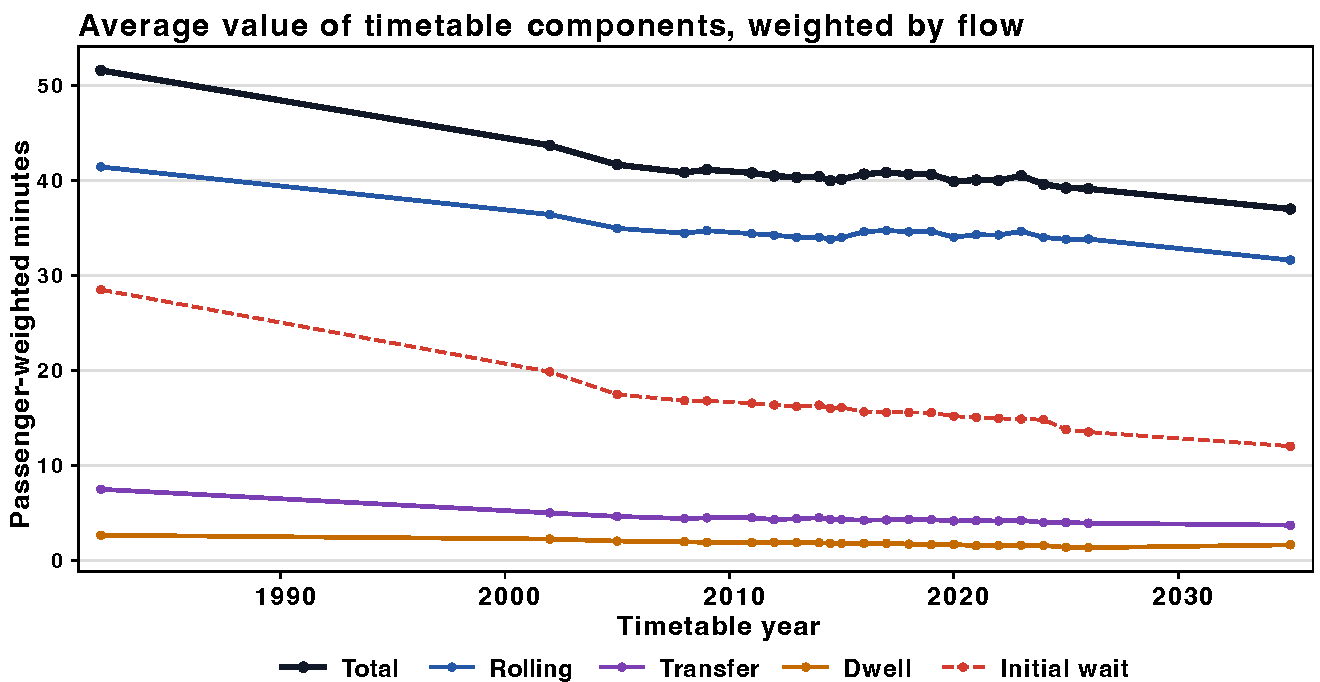
\includegraphics[width=\textwidth]{figures/raw_od_part1_national_component_trends.pdf}
\caption[National historical journey-time trends]{National passenger-weighted historical evolution of total in-system time and its rolling, dwell, transfer, and initial waiting components. Total time excludes initial waiting.}
\label{fig:part1-national-components}
\end{figure}
\newpage
Table~\ref{tab:part1-national-all-years} summarizes the national indicators for the considered timetable years. The main time-component columns are passenger-weighted, while the first numeric column reports the unweighted total-time mean for comparison. Between 1982 and 2026, the average passenger-weighted post-departure travel time for the selected 131-station network falls from 51.60~min to 39.13~min, a reduction of 12.47~min per weighted trip. Initial waiting time falls more strongly, from 28.51~min to 13.53~min. Thus the combined passenger-facing time from random arrival at the station to arrival at the destination falls from 80.11~min in 1982 to 52.66~min in 2026. The 2035 timetable further reduces the post-departure mean to 37.00~min and the initial waiting mean to 12.04~min. The average national headway between departures, defined as double the initial waiting time, is consequently found to have fallen from 57.02~min in 1982 to 27.06~min in 2026. This indicates that station pairs were commonly connected hourly in the 1980s, and half-hourly in the 2020s. The 2035 timetable introduces 15~min headways for additional city pairs, further lowering the national average headway to 24.08~min. A long-term improvement trend is visible in all components. Rolling time falls by 7.59~min between 1982 and 2026, transfer time by 3.56~min, and dwell time by 1.31~min. Initial waiting time falls by 14.98~min. 

Figure~\ref{fig:part1-national-components} portrays these values graphically. Rolling, dwell, transfer and waiting time all decline over time, but not monotonically. The strongest national improvement occurs before the mid-2000s, followed by a plateau of most values, with occasional minor reversals. In 2035, total travel time falls further, owing mostly to lower rolling time. The comparison between weighted and unweighted means in Table~\ref{tab:part1-national-all-years} shows that the improvements are not distributed evenly across all OD pairs. In the passenger-weighted results, 2026 has the lowest observed total post-departure time before 2035. In the unweighted results, however, 2022 is slightly lower than 2026, with 135.00~min compared with 136.04~min. This disparity is due to the different meaning of the two approaches: the unweighted mean gives every OD pair the same importance, including long-distance or low-demand station pairs, whereas the passenger-weighted mean gives proportionally greater importance to OD pairs with higher modelled demand. The finding that 2026 performs better in the weighted mean than in the unweighted mean therefore suggests that recent timetable improvements are concentrated more strongly on OD pairs with larger passenger flows, while some lower-demand pairs are slightly less efficiently connected today than in recent years.

\subsection{Composition of post-departure total time}\label{sec:results-part1-composition}

The component shares in Table~\ref{tab:part1-national-all-years} show how the structure of the average passenger-weighted journey changes over time. In 1982, rolling time accounts for 80.29\% of weighted post-departure time, dwell time for 5.17\%, and transfer time for 14.54\%. By 2026, rolling time accounts for 86.48\%, dwell time for 3.46\%, and transfer time for 10.06\%. The shift toward the rolling corner is shown in Figure~\ref{fig:part1-triangle}. This means that a larger share of the journey is spent in motion rather than in same-train dwell or transfers. Total post-departure time falls while the rolling share rises, so the share increase does not mean that passengers spend more time on trains. Rather, transfer and dwell burdens fall more strongly than in-train movement time. The dwell-share decline until 2026 indicates that dominant weighted paths increasingly avoid long same-train intermediate stops, although this trend reverses slightly by 2035. Most clearly, the transfer share decreases steadily over time, implying increasingly efficient transfers across the country.

\begin{figure}[htbp]
\centering
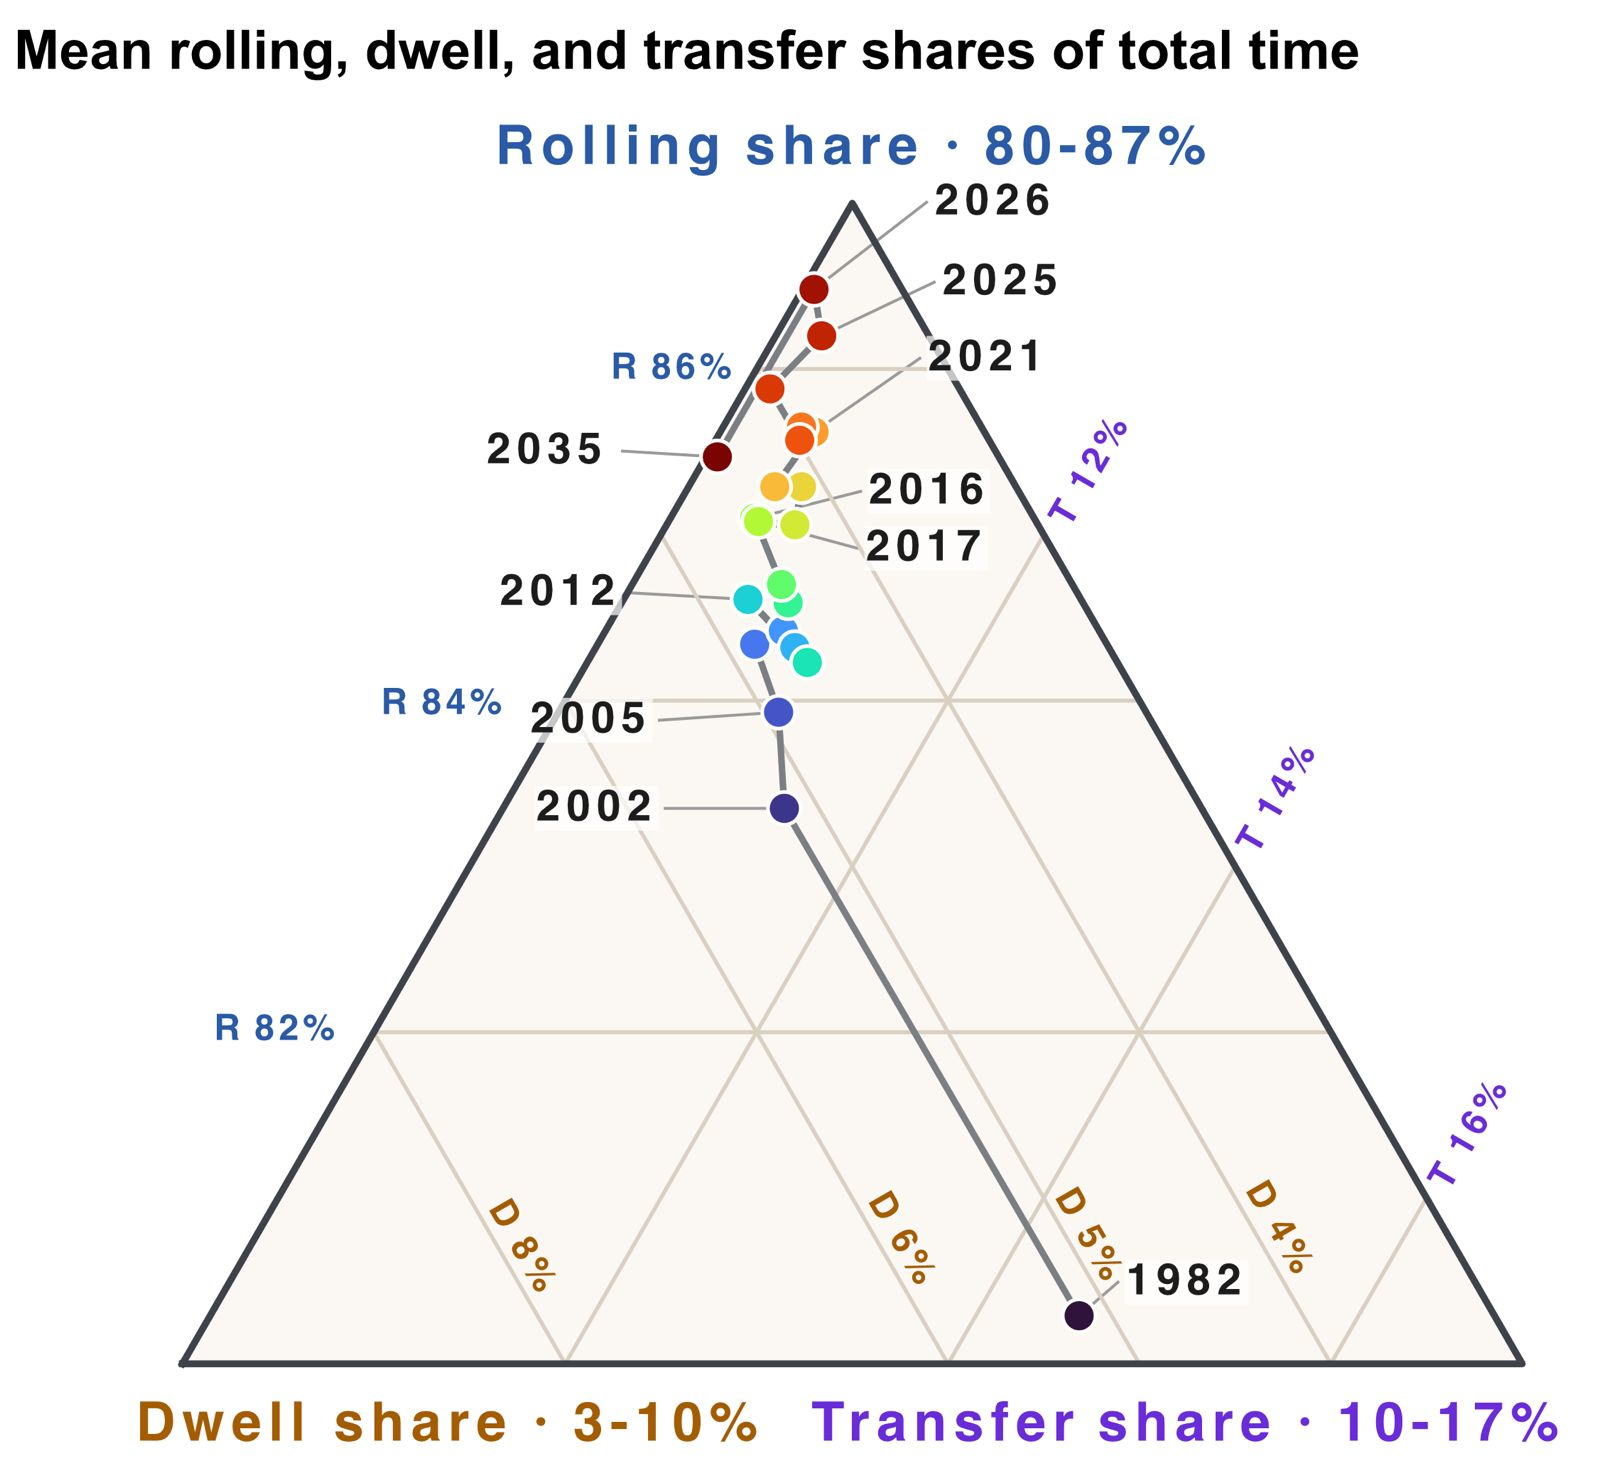
\includegraphics[width=0.62\textwidth]{figures/Triangle.jpeg}
\caption[National historical journey-time composition]{National passenger-weighted composition of in-system time. Each point represents one timetable year in the ternary space spanned by rolling, dwell, and transfer shares.}
\label{fig:part1-triangle}
\end{figure}

\subsection{Spatial progression across cantons}\label{sec:results-part1-spatial-progression}
Figure~\ref{fig:part1-canton-total-time-trends} disaggregates total travel time by origin canton using unweighted OD-pair means. In this calculation, each prepared station-to-station OD pair in the 131-station Part I layer contributes equally, regardless of its estimated passenger flow. The aim of this figure is to show the evolution of the selected national station-pair network at large, and taking unweighted values ensures that station pairs do not shift in importance across years, isolating the effect of individual years' timetable changes. The figure shows a long-term reduction in total time across most cantons, while also making clear that the timing and magnitude of improvements differ strongly by region. The impact of specific infrastructure projects such as the NEAT base tunnels can be identified by sudden drops during their year of introduction (e.g. Ticino, 2017/2021), as well as temporary peaks during construction-impacted years (e.g. Uri, 2020; Schaffhausen, 2024). As Part I considers a selected historical network of 131 stations and 65 named line services, the cantonal graph lines are more sensitive to sudden year-on-year alterations to line stopping patterns or represented line structures than later in Part II.
\begin{figure}[H]
\centering
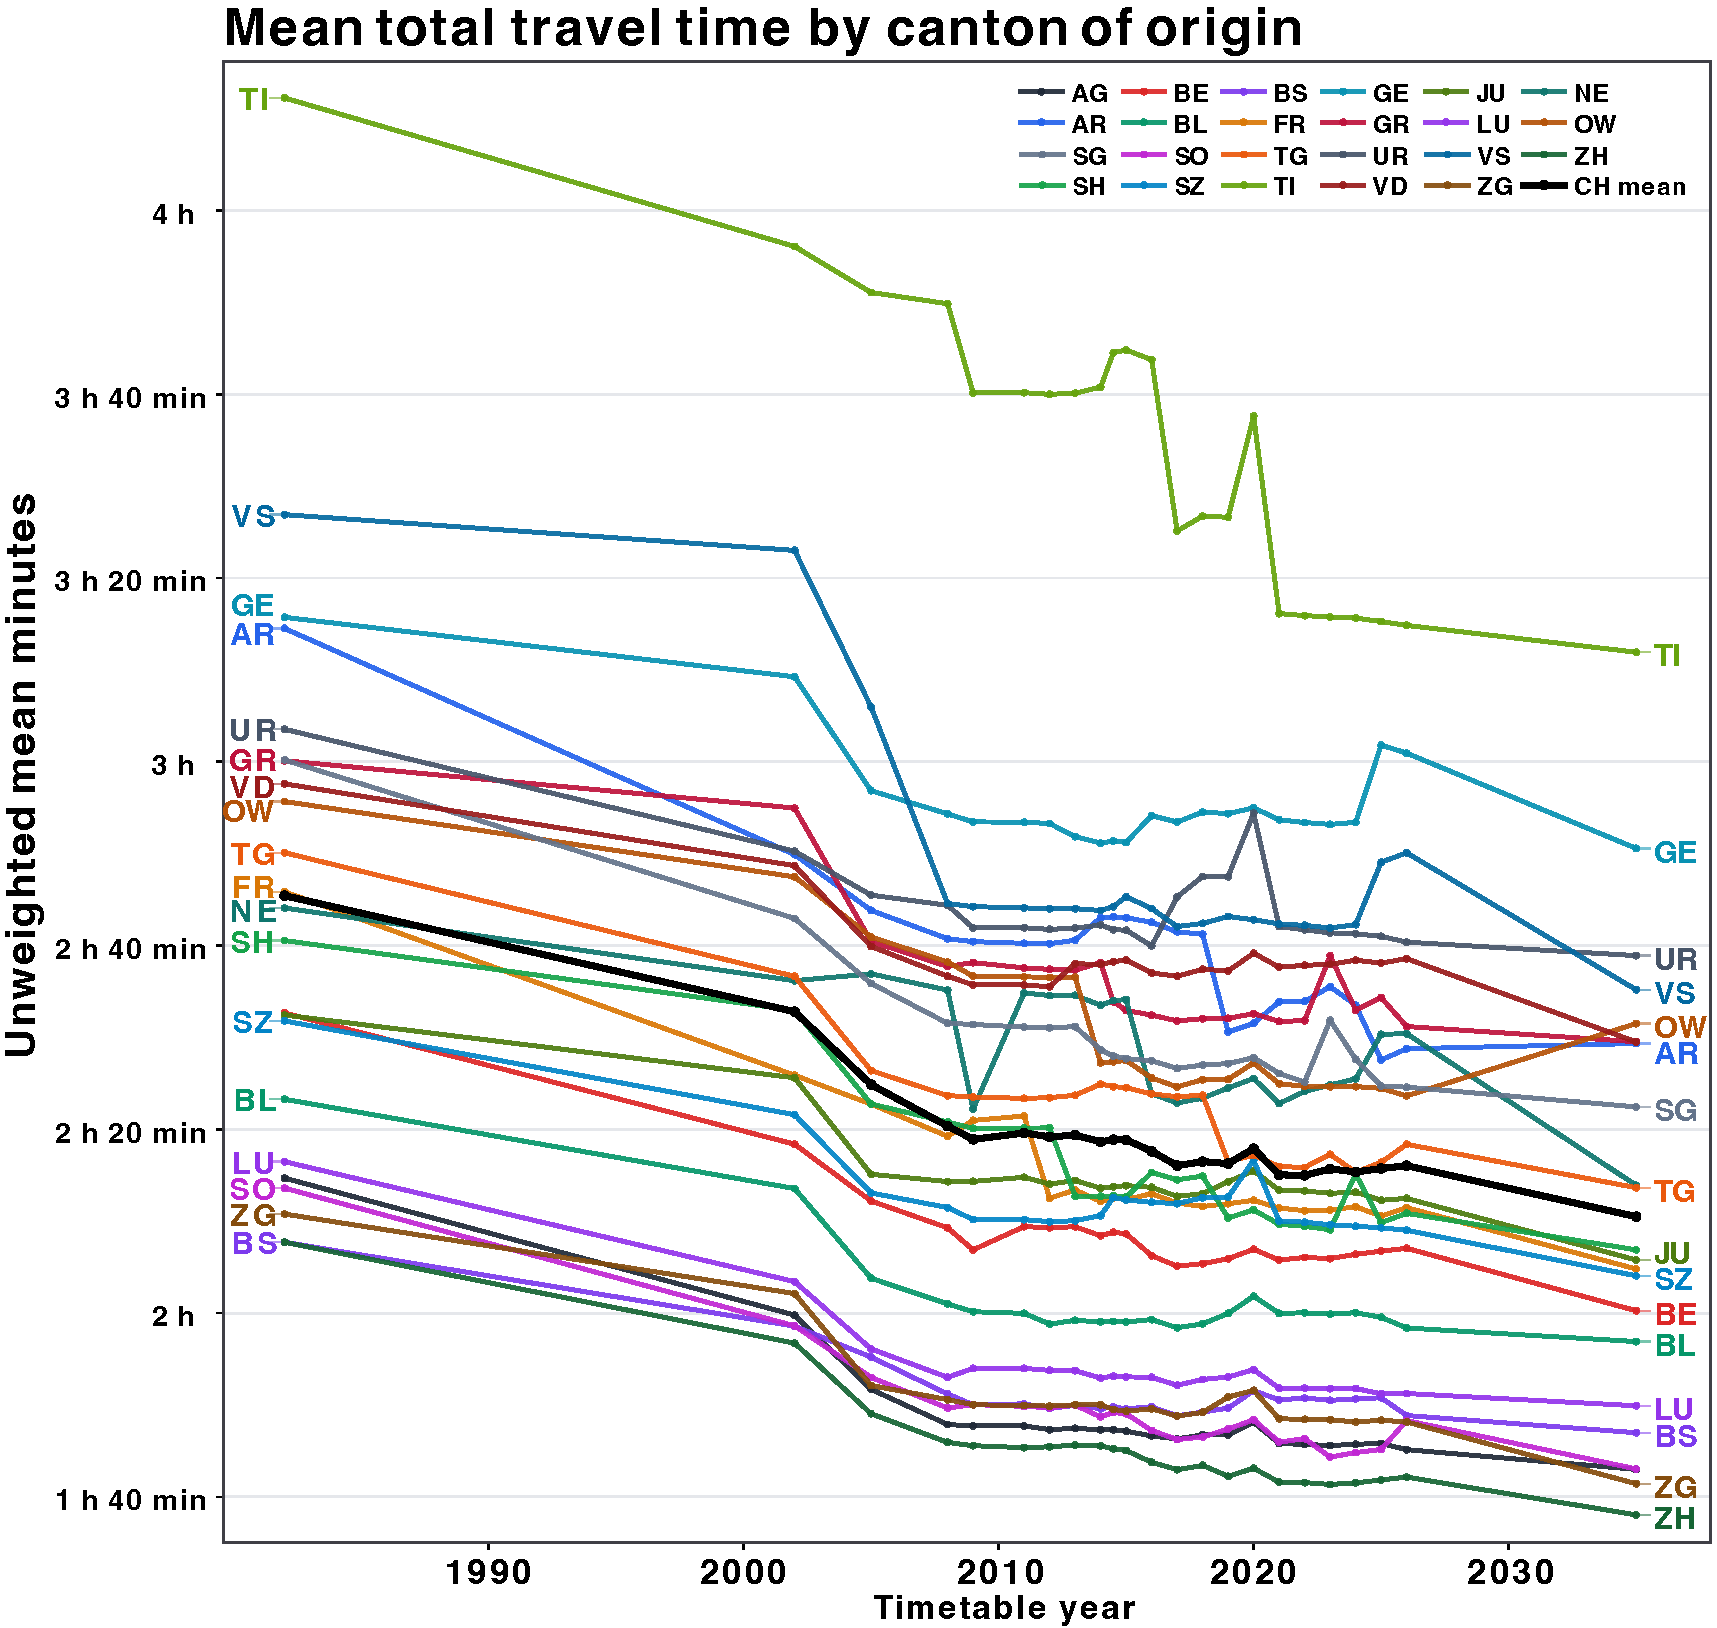
\includegraphics[width=0.75\textwidth]{figures/raw_od_part1_canton_total_time_trends_unweighted_80pct_taller.pdf}
\caption[Total journey time by origin canton]{Unweighted total post-departure travel time by origin canton across Part I's stations and years. Each coloured line represents trips starting in one canton; the black line shows the national unweighted mean. Total time excludes initial waiting time.}

\label{fig:part1-canton-total-time-trends}
\end{figure}

\subsection{Calendar windows and major timetable interventions}\label{sec:results-part1-calendar-windows}

Figure~\ref{fig:part1-event-windows} compares selected timetable windows using unweighted OD-level path metrics. The purpose of this view is to show the spatial breadth of timetable changes across the selected station network, without allowing the largest estimated passenger flows to dominate the interpretation. The heatmap is calculated at the origin-canton level using the endpoint-difference definition introduced in Equation~\eqref{eq:part1-window-delta-unweighted}. Each cell therefore reports the later-year unweighted mean total post-departure time minus the earlier-year value for trips starting in that canton. Negative values indicate lower total time in the later timetable, while positive values indicate a worsening. The values are chronological anchors for interpretation and do not by themselves establish that the named infrastructure or timetable-policy change is the sole cause of the measured change, especially for cantons outside the directly affected corridor.

\paragraph{1982--2002}
The first time window shows the long transformation of the selected network in the lead-up to Bahn 2000. The national unweighted total time falls by 12.63~min. This consists of a 6.63~min reduction in rolling time and a 6.68~min reduction in transfer time, partly offset by a 0.68~min increase in same-train dwell time. Initial waiting time falls by a further 12.65~min. The window therefore captures both faster post-departure movement and a major improvement in service availability. All cantons improve in unweighted total time, but the magnitude varies strongly. The largest cantonal reductions occur for Appenzell Ausserrhoden (24.6~min), Fribourg (20.0~min), St.~Gallen (17.2~min), Ticino (16.2~min), and Solothurn (15.0~min). The smallest reductions occur for Valais (3.9~min), Graubünden (5.2~min), Geneva (6.5~min), Jura (6.8~min), and Schaffhausen (7.6~min).

\begin{figure}[H]
\centering
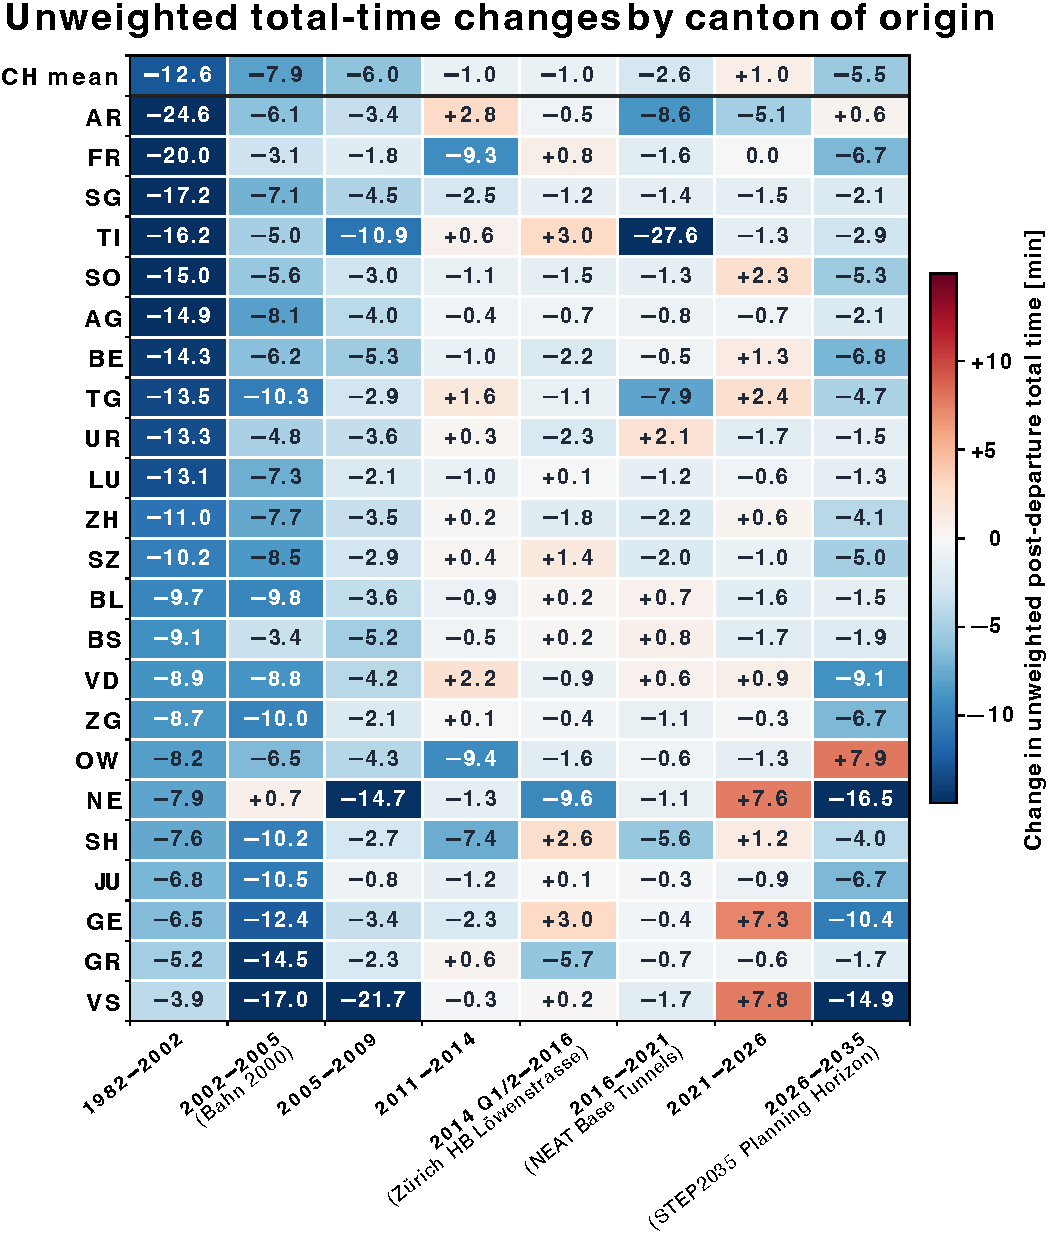
\includegraphics[width=0.76\textwidth]{figures/raw_od_part1_canton_event_window_heatmap_unweighted.pdf}
\caption[Cantonal changes across historical time windows]{Total-time unweighted changes by origin canton across selected historical time windows, with all 131 destinations weighted equally. Each cell is the later-year unweighted mean minus the earlier-year unweighted mean, in minutes. Blue values indicate lower total time in the later timetable, while red values indicate higher total time. The first row gives the national selected-station mean, and cantonal rows describe trips by canton of origin.}
\label{fig:part1-event-windows}
\end{figure}



\paragraph{2002--2005 (Bahn 2000)}
The 2005 timetable is the first modelled timetable after the Bahn 2000 timetable change introduced on 12~December~2004 \citep{sbbRail2000Timetable2004}. The national unweighted total falls by 7.93~min. Rolling time falls by 4.21~min, dwell time by 1.35~min, transfer time by 2.38~min, and initial waiting by 2.73~min. This all-round improvement is consistent with Bahn 2000's role as a national timetable and node-connection programme. The strongest cantonal reductions are in Valais (17.0~min), Graubünden (14.5~min), Geneva (12.4~min), Jura (10.5~min), and Thurgau (10.3~min). Neuchâtel is the only exception, worsening slightly by 0.7~min. At station level, Hohtenn, Ausserberg, and Eggerberg improve by more than 37~min, while the largest station-level worsening is Bulle (+19.3~min).

\paragraph{2005--2009}
This time window covers the first represented years after the Lötschberg Base Tunnel entered full commercial service at the 2008 timetable change \citep{blsLoetschbergHistory}. The national unweighted total falls by 5.96~min, driven mainly by a 5.01~min reduction in rolling time. Dwell time falls by 0.86~min, transfer time changes only slightly by 0.09~min, and initial waiting is almost unchanged. The strongest cantonal reductions are in Valais (21.7~min), Neuchâtel (14.7~min), Ticino (10.9~min), Bern (5.3~min), and Basel-Stadt (5.2~min). No cantons worsen overall in this window of time. The station-level pattern makes the infrastructure effect more visible: Visp, Leuk, Sierre/Siders, Sion, and Brig improve most strongly, while Kandersteg, Goppenstein, and Frutigen are among the weakest origins. This follows the expected base-tunnel opening pattern: faster long-distance axes improve many long-distance pairs, while some stations tied to the older mountain-line structure lose their relative timetable advantage.

\paragraph{2011--2014}
The 2011--2014 Q1/2 interval describes the period immediately before the opening of Zürich HB's underground platforms. The national unweighted total falls by 0.97~min, with reductions of 0.57~min in rolling time, 0.23~min in dwell time, 0.17~min in transfer time, and 0.64~min in initial waiting. The canton rows show moderate regional differences: Obwalden improves by 9.4~min, Fribourg by 9.3~min and Schaffhausen by 7.4~min, while the largest worsening is in Appenzell Ausserrhoden (+2.8~min), followed by Vaud (+2.2~min) and Thurgau (+1.6~min). At station level, Bulle, Sarnen and Altstätten SG improve most strongly, while Palézieux, Nyon and Morges experience longer total travel times.

\paragraph{2014--2016 (Zürich HB Löwenstrasse)}
This time window covers both stages of the Zürich Durchmesserlinie. SBB and ZVV put the Löwenstrasse underground station and the Weinberg tunnel into operation on 15~June~2014, initially routing S-Bahn lines through the new cross-city link \citep{sbbZuerichDml2014TimetableChange}, followed by long-distance traffic at the end of 2015 \citep{zvvDurchmesserlinieProject}. Nationally, the unweighted total falls by 1.02~min. Rolling time rises by 0.42~min, while dwell time falls by 0.26~min and transfer time by 1.18~min. Initial waiting falls by 0.91~min. The main observed benefit of this window is therefore the transfer-time reduction, likely attributable to the optimization of the Zürich HB node. The largest cantonal improvements are in Neuchâtel (9.6~min) and Graubünden (5.7~min), and the most worsened cantons are Geneva (+3.0~min), Ticino (+3.0~min) and Schaffhausen (+2.6~min). Sonceboz-Sombeval, La Chaux-de-Fonds and Courtelary all improve strongly. The largest worsened origins include Chiasso, Biberbrugg and Neuhausen.

\paragraph{2016--2021 (Gotthard Axis Base Tunnels)}
This time window compares the final pre-Gotthard Base Tunnel modelled timetable with the first represented timetable after the Ceneri Base Tunnel entered regular operation: the Gotthard Base Tunnel commenced regular timetable operations in December~2016, and the Ceneri Base Tunnel in December~2020 \citep{edaGotthardOpening2016,railwayNewsCeneri2020}. The national unweighted total falls by 2.57~min. Rolling time falls by 1.57~min, dwell time by 0.85~min, and transfer time by 0.15~min, while initial waiting increases by 0.38~min. The spatial effect is dominated by the north--south axis: Ticino improves by 27.6~min. The main worsened canton is Uri (+2.1~min), due in large part to being skipped by all IC trains in the 2021 timetable. At station level, Chiasso, Lugano, Bellinzona, and Biasca show very large improvements, while the largest worsened station origins include Airolo, Faido and Göschenen. This pattern again illustrates how the NEAT base-tunnel programme improved the main cisalpine corridor while increasing travel time for several origins along the old route.

\paragraph{2021--2026}
The 2021--2026 time window is the only interval in Figure~\ref{fig:part1-event-windows} where the national unweighted total worsens, increasing by 1.00~min. Rolling time increases by 1.32~min and transfer time by 0.38~min, while dwell time falls by 0.70~min and initial waiting falls by 1.72~min. This means that many OD pairs have more frequent or better-spaced departures, but many post-departure paths become slower after boarding. The window includes the 2025 Romandie timetable retiming change, which SBB described as a punctuality-oriented change and the largest timetable change in western Switzerland since Bahn 2000 \citep{sbbRomandie2025Punctuality}. Its intent was to lengthen some travel times and add timetable buffer, thereby making the affected areas more robust in the face of delays. At the same time, the new node at Renens~VD was inaugurated, making several transfers more efficient. The strongest cantonal improvements are in Appenzell Ausserrhoden (5.1~min), Basel-Stadt (1.7~min) and Uri (1.7~min), while the strongest worsened cantons are Valais (+7.8~min), Neuchâtel (+7.6~min) and Geneva (+7.3~min). As an example, Morges--Yverdon-les-Bains worsens its total time from 27.12~min in 2021 to 44.00~min in 2026, but its initial waiting time improves from 19.32~min to 14.50~min. Lausanne--Genève rises from 39.58~min to 42.75~min, but its initial waiting time falls from 7.57~min to 5.42~min. These examples show that this robustness-oriented timetable change worsened some total travel times, but concurrently managed to lower initial waiting times, substantially improving the average headway.

\paragraph{2026--2035 (STEP 2035 Planning Horizon)}
The final time window compares the 2026 timetable with the STEP 2035 planning horizon \citep{sbbStep2035}. The national unweighted total is projected to fall by 5.55~min. Rolling time falls by 4.86~min and transfer time by 2.09~min, while dwell time rises by 1.40~min. Initial waiting falls by 2.30~min. The strongest cantonal gains are in Neuchâtel (16.5~min), Valais (14.9~min), Geneva (10.4~min), Vaud (9.1~min), and Bern (6.8~min). All but two cantons improve, with Obwalden worsening by 7.9~min and Appenzell Ausserrhoden by 0.6~min. At station level, the largest improvements occur at Leuk, Le Locle, La Chaux-de-Fonds and Sion, while the largest worsened origins include Zofingen, Palézieux and Sarnen. STEP 2035 is therefore associated with broad time savings, especially in western and southern Switzerland, with a total effect similar to the 2005--2009 window, albeit with two instead of no worsened cantons. Many of the negative spatially concentrated effects of the 2021--2026 window are expected to reverse by 2035.

\subsection{Best timetabled year by canton}\label{sec:results-part1-2026-best}

Figure~\ref{fig:part1-canton-best-past-total-time-year} compares the best observed pre-2035 total-time year by canton of origin under two aggregation assumptions. In the unweighted map, each OD pair contributes equally, so the map is more sensitive to peripheral and long-distance relations. In the passenger-weighted map, high-demand OD pairs have greater influence, shifting several cantons toward years in which major passenger flows perform best. The black-circled canton labels indicate cases where 2035 is lower than the best observed 1982--2026 value; for these cantons, the mapped colour therefore represents the best non-future year rather than the absolute best year across all considered timetables. Older years are more common in the passenger-weighted panel. Ticino is an instructive example: its best observed weighted year is 2002, despite later major north--south infrastructure improvements. This likely occurs because the demand model responds to improved generalized costs: later base-tunnel years make longer-distance trips more attractive, changing the destination mix of trips starting in Ticino. The average over all weighted destinations may therefore rise in subsequent years, despite direct north--south OD paths becoming much faster.

\begin{figure}[htbp]
\centering
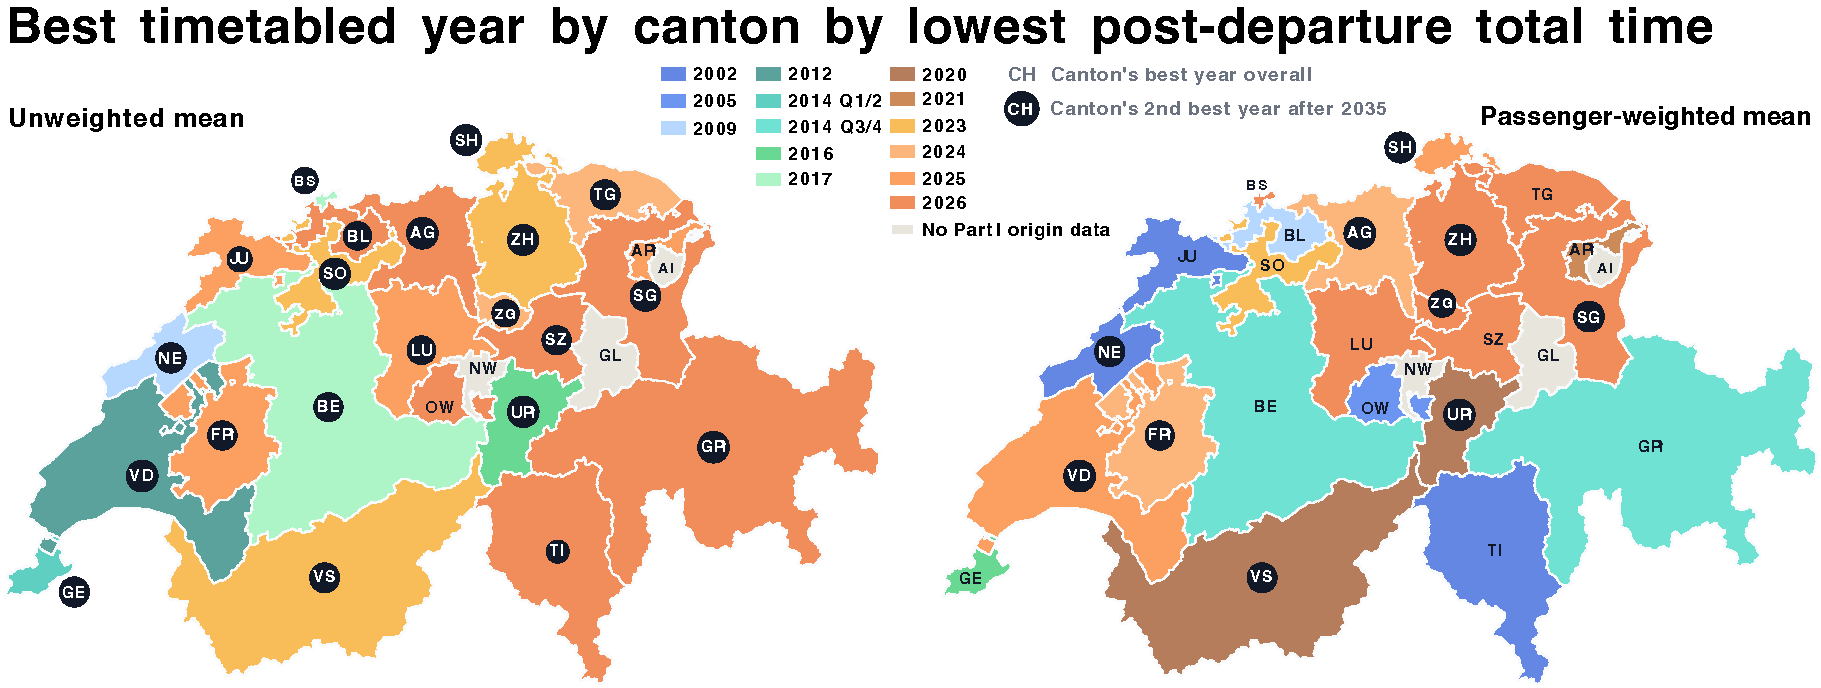
\includegraphics[width=\textwidth]{figures/raw_od_part1_canton_best_total-time_year.pdf}
\caption[Best historical timetable year by canton]{Best past total-time year by canton of origin. The left panel shows the unweighted mean, while the right panel shows the passenger-weighted mean. Colours indicate the best observed timetable year between 1982 and 2026. Plain canton labels indicate that the coloured year is the canton's best year overall; white labels in black circles indicate that 2035 is lower still.}
\label{fig:part1-canton-best-past-total-time-year}
\end{figure}
\newpage
\section{Discussion I}\label{sec:discussion-part1}

\subsection{National time reductions}\label{sec:discussion-part1-main}

The first main finding is that the reconstructed Swiss long-distance timetables become substantially more passenger-efficient over the studied period. Between 1982 and 2026, passenger-weighted post-departure time falls from 51.60 to 39.13 minutes per trip, while initial waiting falls from 28.51 to 13.53 minutes. Rolling, dwell, transfer, and waiting times all decline over the full period, although not monotonically. The result therefore captures more than faster trains: it also reflects higher service frequency, shorter same-train stops, and better transfer coordination within complete journeys.

The component-share analysis indicates that by 2026, a larger share of the passenger-weighted total journey time is spent moving, while dwell and transfer shares are lower. Since absolute rolling time also falls, this does not imply longer on-board journeys. Instead, a larger share of a shorter journey consists of movement toward the destination, increasing timetable efficiency. This is a meaningful sign of timetable quality: passengers spend increasingly less of their journey in the comparatively unproductive and unfavourable states of waiting during a transfer or sitting through long same-train intermediate stops.

\subsection{Weighted vs. unweighted results}\label{sec:discussion-part1-weighting}

The weighted and unweighted results answer related but different questions. The passenger-weighted result asks what the timetable looks like for the station pairs that the model estimates to be actually used by passengers. It is therefore the most relevant measure for passenger-minute exposure. The unweighted result asks what the timetable looks like across the selected station-pair set as a geometry of possible OD pairs. It is more sensitive to peripheral, low-demand, and long-distance pairs, but more accurately serves as a consistent baseline on which the schedule timing changes can be depicted and compared across timetable years.

This difference explains why 2026 is the best observed year in the national passenger-weighted results before 2035, while the unweighted results reach a slightly better value in 2022. The largest passenger flows benefit enough from the 2026 timetable to pull the weighted mean down, while some lower-flow or peripheral OD pairs are connected less efficiently than in earlier years. For a policy interpretation, the two measures are complementary. The weighted result is appropriate for assessing expected passenger exposure, while the unweighted result is useful for detecting spatial equity issues and timetable regressions at network edges. The best-year map makes this visible: many cantons today appear close to their best state when every station pair is treated equally, while others show lower average total times once demand is considered.

\subsection{Infrastructure effects}\label{sec:discussion-part1-infrastructure}

Infrastructure project effects influence the model, but must be interpreted at the correct spatial scale. The Lötschberg, Gotthard, and Ceneri base-tunnel windows show the expected improvements on their main long-distance axes. In the NEAT base tunnel time window, Ticino improves strongly in the unweighted canton heatmap, and the station-level pattern shows large improvements for Chiasso, Lugano, Bellinzona, and Biasca. These results are consistent with the intended function of the base tunnels.

At the same time, the benefits are not spatially uniform. A base tunnel shortens a through corridor and reorganizes the timetable around a new fast route. This can reduce the relative accessibility of older mountain-line stations or intermediate origins that are no longer served by the fastest trains. Airolo, Faido, and Göschenen are a few examples of this: their worsened aggregate values indicate that their accessibility geography changed. The same principle was observed in Lötschberg-line stations such as Kandersteg, Goppenstein, and Frutigen. Direct corridor improvements and origin-level redistribution can occur at the same time.

\subsection{Robustness and retiming potential}\label{sec:discussion-part1-romandie}

The 2021--2026 window is important because it is the only selected interval in which the national unweighted total time worsens, driven mainly by the controversial 2025 Romandie timetable relaxation. This unweighted worsening coexists with a slight observed reduction in passenger-weighted total time and waiting time, indicating that the 2026 timetable performs particularly well for major flows, while lower-flow station pairs experience longer post-boarding journey times on average. Morges--Yverdon-les-Bains and Lausanne--Genève both show higher post-boarding time in 2026 but improved headways between services due to revamped connections. From a passenger's perspective, the timetable therefore offers more frequent or better-spaced services, despite lengthening in-vehicle time. Added running-time buffers can therefore make a timetable more robust and delay-resistant, but slower. Since this thesis does not model delay propagation, missed connections under disruption, or reliability benefits, it measures only the scheduled travel-time side of this trade-off. The model can therefore identify where scheduled travel time worsens, but it cannot determine whether the real-world reliability gain compensates passengers for that scheduled increase.

The local reversals identified in Part I motivate Part II, which is focused on optimizing 2026 and 2035's timetables. The historical results show that Swiss timetable development has already delivered large improvements through the cascading effects of faster infrastructure, higher frequencies, and better synchronization. On the other hand, they also show that a strong national timetable can still contain OD-specific penalties caused by transfer misalignment. These are the situations where small retimings may be useful: If an OD pair is slow because of a long transfer or a narrowly missed connection, a small local timetable adjustment may reduce passenger-minutes without requiring a new infrastructure project, provided it does not negatively impact neighbouring lines. In Part II's optimization, the objective will be to identify specific timing relationships whose minimally disruptive adjustment could improve high-impact connections while preserving the existing periodic timetable structure, line services and node patterns.

\subsection{Limitations of the Part I interpretation}\label{sec:discussion-part1-limitations}

Several limitations should be kept in mind. First, the historical timetable is represented as a repeating two-hour pattern and does not include peak-only services. Some real-world improvements that occur only in peak periods (such as 2026's IC 57) are therefore outside the model. Second, the 131-station layer focuses on nationally important standard-gauge stations and does not represent the full local and regional access system. This is particularly relevant for mountain-line stations and municipalities where feeder buses, narrow-gauge railways, or local stopping services are closely tied to the demand expected in a region.

Third, the year-specific OD matrices are modelled rather than observed for every year. They are anchored in NPVM 2023 and then projected with generalized-cost and population adjustments. Because of this, the results must only be read as modelled timetable indicators. Fourth, spatial aggregates combine timetable change and demand-composition change in the passenger-weighted view. This is appropriate for passenger-exposure interpretation, but it can obscure direct route improvements. Direct OD checks remain necessary when interpreting infrastructure effects, so the dataset used in this thesis may be used to generate individual statistics and numerical analyses as needed. Finally, the model is deterministic and schedule-based. It does not include reliability, crowding, fares, punctuality, rolling-stock circulation, platform occupation, or crew constraints. These exclusions are especially relevant for robustness-oriented timetable optimizations, which are out of scope of this thesis.

\clearpage
\part{Matheuristic Event-Retiming Optimization}\label{sec:part2}
\section{Methods II}\label{sec:methods-part2}
Part II moves from the smaller historical reconstruction in Part I to a far more detailed representation of the full Swiss passenger rail periodic timetable in 2026 and 2035. Its purpose is to test whether small integer-minute timetable retimings can reduce passenger-weighted post-departure travel time in a minimally intrusive way, preserving the overall structure of the baseline timetable. The model compares four scenarios for each year: Baseline, Optimized Step~1, Optimized Step~2, and Optimized Step~3. The 2026 network contains 1'592 stations, while the 2035 network contains 1'579. The timetable representation contains 255 named line-service rows in both the baseline and final optimized timetable, compared with 65 line-service rows in the historical Part~I timetable. Table~\ref{tab:timetable-representations} compares the scope of the two parts further. Analogous to Figure~\ref{fig:part1-workflow}, Figure~\ref{fig:part2-workflow} summarizes the Part~II workflow.

\begin{figure}[htbp]
\centering
\resizebox{0.98\textwidth}{!}{%
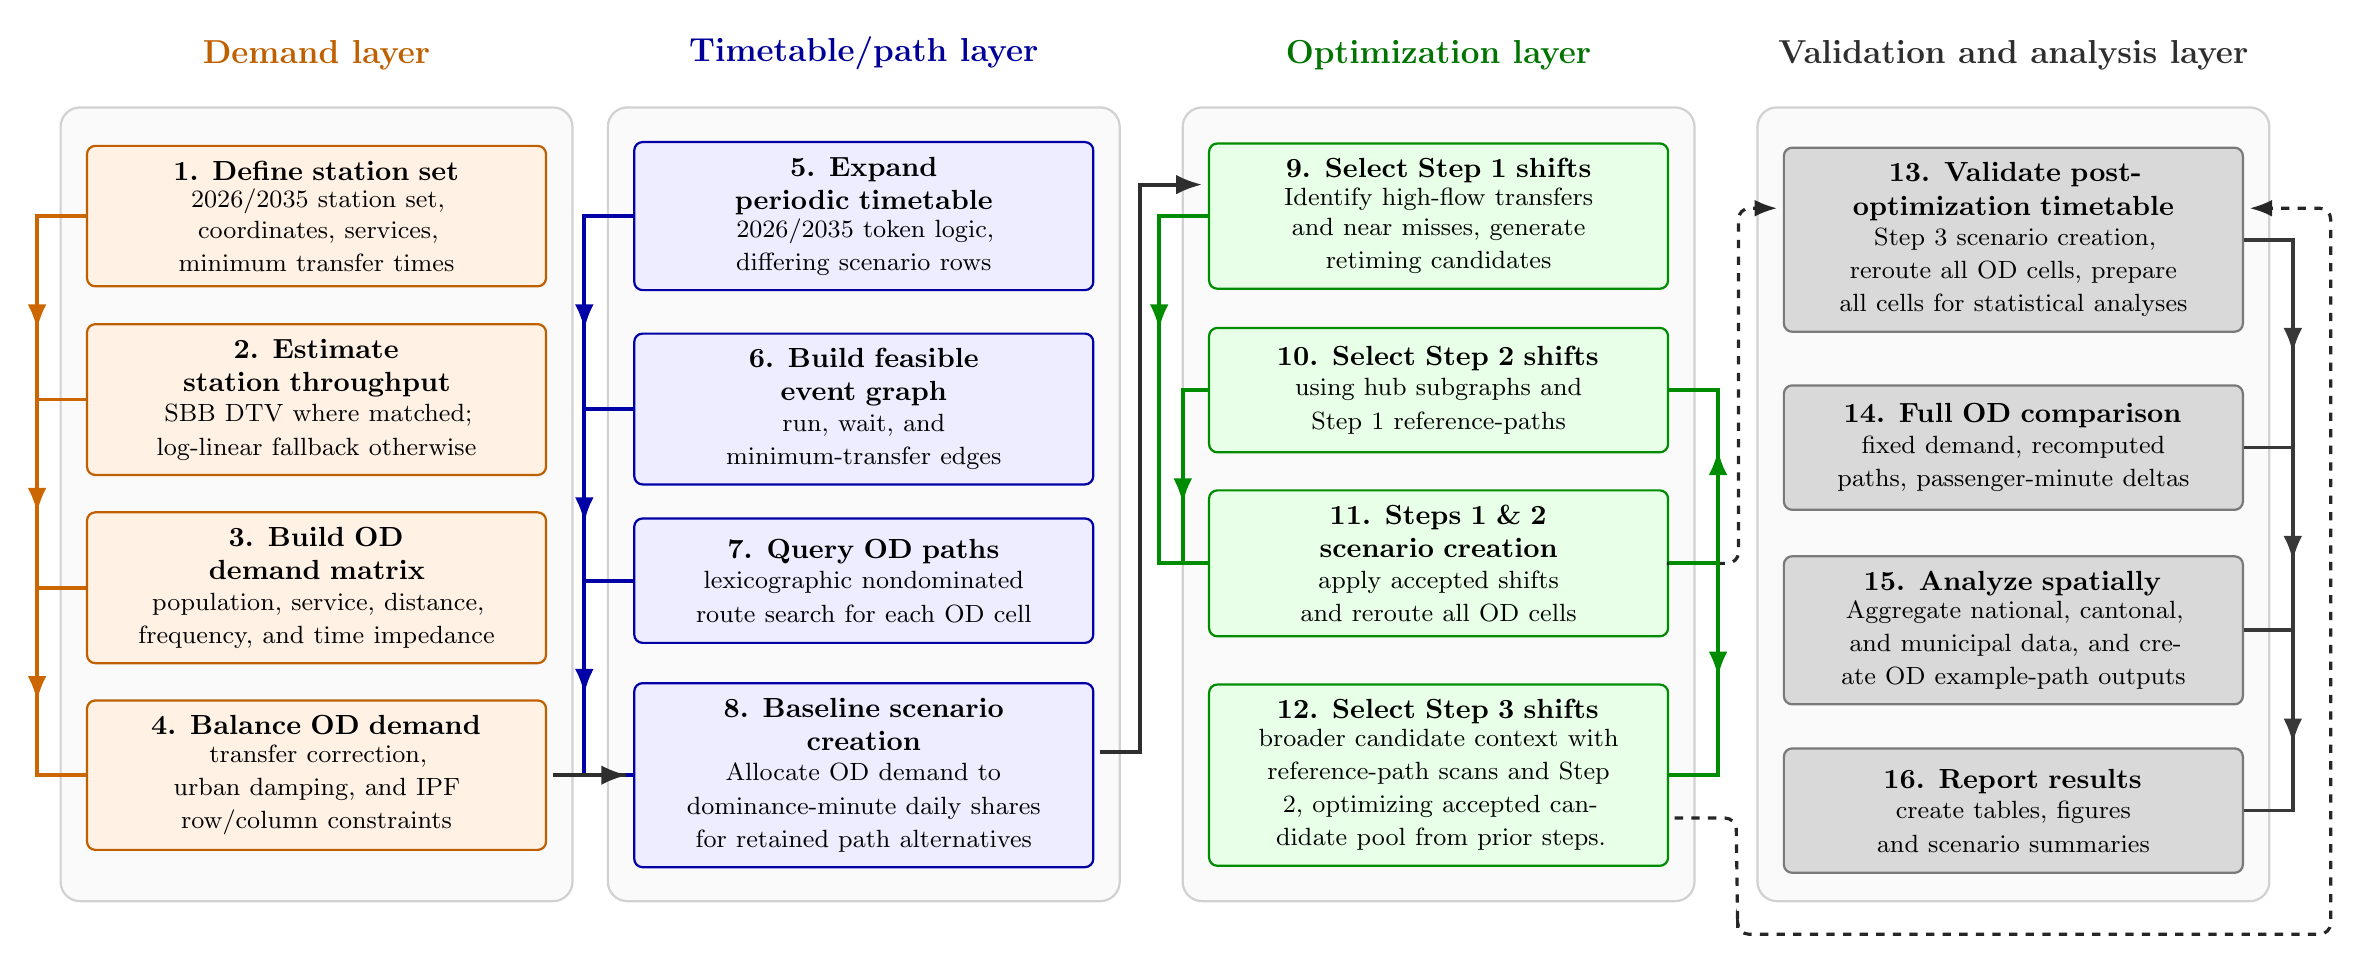
\begin{tikzpicture}[
    font=\normalsize,
    >=Latex,
    box/.style={
        rectangle,
        rounded corners=3pt,
        draw=black!55,
        line width=0.8pt,
        align=center,
        text width=5.45cm,
        minimum height=1.58cm,
        inner sep=5.4pt
    },
    demandbox/.style={
        box,
        fill=orange!10,
        draw=orange!75!black
    },
    pathbox/.style={
        box,
        fill=blue!7,
        draw=blue!65!black
    },
    optbox/.style={
        box,
        fill=green!9,
        draw=green!55!black
    },
    validationbox/.style={
        box,
        fill=gray!30,
        draw=gray!95!black
    },
    lane/.style={
        rounded corners=7pt,
        draw=black!18,
        line width=0.8pt,
        fill=black!2
    },
    lanetitle/.style={
        font=\large\bfseries,
        anchor=south
    },
    joinarrow/.style={
        ->,
        >=Latex,
        line width=1.45pt,
        draw=black!82,
        shorten >=2pt,
        shorten <=2pt
    },
    feedback/.style={
        ->,
        >=Latex,
        line width=1.15pt,
        draw=black!85,
        dashed,
        rounded corners=4pt,
        shorten >=2pt,
        shorten <=2pt
    }
]

% ---------------------------------------------------------------------
% Part-I-style side connectors
% ---------------------------------------------------------------------

\def\sideleft#1#2#3{%
    \draw[line width=1.35pt, draw=#1]
        (#2.west) -- ++(-0.62,0) |- (#3.west);
    \draw[->, >=Latex, line width=1.35pt, draw=#1]
        ($ (#2.west) + (-0.62,-0.96) $) -- ++(0,-0.48);
}
\def\sideleftclose#1#2#3{%
    \draw[line width=1.35pt, draw=#1]
        (#2.west) -- ++(-0.32,0) |- (#3.west);
    \draw[->, >=Latex, line width=1.35pt, draw=#1]
        ($ (#2.west) + (-0.32,-0.96) $) -- ++(0,-0.48);
}

\def\sideright#1#2#3{%
    \draw[line width=1.35pt, draw=#1]
        (#2.east) -- ++(0.62,0) |- (#3.east);
    \draw[->, >=Latex, line width=1.35pt, draw=#1]
        ($ (#2.east) + (0.62,-0.96) $) -- ++(0,-0.48);
}
\def\siderightup#1#2#3{%
    \draw[line width=1.35pt, draw=#1]
        (#2.east) -- ++(0.62,0) |- (#3.east);
    \draw[->, >=Latex, line width=1.35pt, draw=#1]
        ($ (#2.east) + (0.62,+0.96) $) -- ++(0,+0.48);
}
\def\siderightclose#1#2#3{%
    \draw[line width=1.35pt, draw=#1]
        (#2.east) -- ++(0.32,0.0) |- (#3.east);
    \draw[->, >=Latex, line width=1.35pt, draw=#1]
        ($ (#2.east) + (0.32,+0.96) $) -- ++(0,+0.48);
}

% ---------------------------------------------------------------------
% Column and row coordinates
% ---------------------------------------------------------------------

\def\xD{0}
\def\xP{6.95}
\def\xO{14.25}
\def\xA{21.55}

\def\yOne{-0.2}
\def\yTwo{-2.65}
\def\yThree{-4.83}
\def\yFour{-7.3}

\def\laneTop{1.18}
\def\laneBottom{-8.90}
\def\laneHalfWidth{3.25}

\pgfmathsetmacro{\xvalidationLoop}{\xA+\laneHalfWidth+0.78}
\pgfmathsetmacro{\xOptLoop}{\xO+\laneHalfWidth+0.55}
\pgfmathsetmacro{\yLoop}{\laneBottom-0.42}

% ---------------------------------------------------------------------
% Lane backgrounds
% ---------------------------------------------------------------------

\begin{pgfonlayer}{background}
    \draw[lane]
        (\xD-\laneHalfWidth,\laneTop)
        rectangle
        (\xD+\laneHalfWidth,\laneBottom);

    \draw[lane]
        (\xP-\laneHalfWidth,\laneTop)
        rectangle
        (\xP+\laneHalfWidth,\laneBottom);

    \draw[lane]
        (\xO-\laneHalfWidth,\laneTop)
        rectangle
        (\xO+\laneHalfWidth,\laneBottom);

    \draw[lane]
        (\xA-\laneHalfWidth,\laneTop)
        rectangle
        (\xA+\laneHalfWidth,\laneBottom);
\end{pgfonlayer}

% ---------------------------------------------------------------------
% Lane titles
% ---------------------------------------------------------------------

\node[lanetitle, text=orange!75!black] at (\xD,\laneTop+0.35)
{Demand layer};

\node[lanetitle, text=blue!60!black] at (\xP,\laneTop+0.35)
{Timetable/path layer};

\node[lanetitle, text=green!45!black] at (\xO,\laneTop+0.35)
{Optimization layer};

\node[lanetitle, text=black!82] at (\xA,\laneTop+0.35)
{Validation and analysis layer};

% ---------------------------------------------------------------------
% Demand layer: 1--4
% ---------------------------------------------------------------------

\node[demandbox] (d1) at (\xD,\yOne) {
    \textbf{1. Define station set}\\[-1pt]
    \small 2026/2035 station set,\\ coordinates, services, \\minimum transfer times
};

\node[demandbox] (d2) at (\xD,\yTwo+0.12) {
    \textbf{2. Estimate \\station throughput}\\[-1pt]
    \small SBB DTV where matched; log-linear fallback otherwise
};

\node[demandbox] (d3) at (\xD,\yThree-0.09) {
    \textbf{3. Build OD \\demand matrix}\\[-1pt]
    \small population, service, distance, frequency, and time impedance
};

\node[demandbox] (d4) at (\xD,\yFour) {
    \textbf{4. Balance OD demand}\\[-1pt]
    \small transfer correction, \\urban damping, and IPF row/column constraints
};

% ---------------------------------------------------------------------
% Timetable/path layer: 5--8
% ---------------------------------------------------------------------

\node[pathbox] (p5) at (\xP,\yOne) {
    \textbf{5. Expand \\periodic timetable}\\[-1pt]
    \small 2026/2035 token logic,\\ differing scenario rows
};

\node[pathbox] (p6) at (\xP,\yTwo-0.0) {
    \textbf{6. Build feasible\\ event graph}\\[-1pt]
    \small run, wait, and minimum-transfer edges
};

\node[pathbox] (p7) at (\xP,\yThree-0.) {
    \textbf{7. Query OD paths}\\[-1pt]
    \small lexicographic nondominated route search for each OD cell
};

\node[pathbox] (p8) at (\xP,\yFour) {
    \textbf{8. Baseline scenario \\creation}\\[-1pt]
    \small Allocate OD demand to dominance-minute daily shares for retained path alternatives
};

% ---------------------------------------------------------------------
% Optimization layer: 9--12
% ---------------------------------------------------------------------

\node[optbox] (o9) at (\xO,\yOne) {
    \textbf{9. Select Step 1 shifts}\\[-1pt]
    \small Identify high-flow transfers and near misses, generate\\ retiming candidates
};

\node[optbox] (o10) at (\xO,\yTwo+0.24) {
    \textbf{10. Select Step 2 shifts}\\[-1pt]
    \small using hub subgraphs and Step~1 reference-paths
};

\node[optbox] (o11) at (\xO,\yThree+0.22) {
    \textbf{11. Steps 1 \& 2\\ scenario creation}\\[-1pt]
    \small apply accepted shifts and reroute all OD cells
};

\node[optbox] (o12) at (\xO,\yFour) {
    \textbf{12. Select Step 3 shifts}\\[-1pt]
    \small broader candidate context with \\ reference-path scans and Step 2, optimizing accepted candidate pool from prior steps.
};

% ---------------------------------------------------------------------
% Rebuild and analysis layer: 13--16
% ---------------------------------------------------------------------

\node[validationbox] (a13) at (\xA,\yOne-0.3) {
    \textbf{13. Validate post-optimization timetable}\\[-1pt]
    \small Step 3 scenario creation, reroute all OD cells, prepare all cells for statistical analyses
};

\node[validationbox] (a14) at (\xA,\yTwo-0.49) {
    \textbf{14. Full OD comparison}\\[-1pt]
    \small fixed demand, recomputed paths, passenger-minute deltas
};

\node[validationbox] (a15) at (\xA,\yThree-0.63) {
    \textbf{15. Analyze spatially}\\[-1pt]
    \small Aggregate national, cantonal, \\and municipal data, and create OD example-path outputs
};

\node[validationbox] (a16) at (\xA,\yFour-0.45) {
    \textbf{16. Report results}\\[-1pt]
    \small create tables, figures and scenario summaries
};

% ---------------------------------------------------------------------
% Internal lane arrows
% ---------------------------------------------------------------------

\sideleft{orange!80!black}{d1}{d2}
\sideleft{orange!80!black}{d2}{d3}
\sideleft{orange!80!black}{d3}{d4}

\sideleft{blue!65!black}{p5}{p6}
\sideleft{blue!65!black}{p6}{p7}
\sideleft{blue!65!black}{p7}{p8}

\sideleft{green!55!black}{o9}{o11}
\sideleftclose{green!55!black}{o10}{o11}


% validation arrows are placed on the right to keep the left side clear
% for black cross-layer validation arrows.
\draw[feedback]
    ($(o11.east)+(-0.1,0.0)$)
    -- ++(0.98,0)
    |- ($(a13.west)+(0,0.40)$);

\siderightup{green!55!black}{o11}{o10}
\sideright{green!55!black}{o11}{o12}

\sideright{black!78}{a13}{a14}
\sideright{black!78}{a14}{a15}
\sideright{black!78}{a15}{a16}

% ---------------------------------------------------------------------
% Cross-layer workflow arrows
% ---------------------------------------------------------------------

\draw[joinarrow]
    (d4.east)
    -- ++(1,0)
    |- ($(p8.west)$);

\draw[joinarrow]
    ($(p8.east)+(0,0.30)$)
    -- ++(0.58,0)
    |- ($(o9.west)+(0,0.40)$);



% Step 1 validation seeds the second, more exact search.
% The dashed feedback arrow is routed outside the validation lane.
\draw[feedback]
    ($(o12.south east)+(0,0.62)$)
    -- ++(0.85,0)
    -- (\xOptLoop,\yLoop)
    |- (\xvalidationLoop,\yLoop)

    |- ($(a13.east)+(0,0.40)$);

\end{tikzpicture}%
}
\caption[Part II modelling and retiming workflow]{Part II modelling and retiming workflow. The demand layer constructs year-specific OD demand, the timetable/path layer expands the 2026 and 2035 timetables and allocates demand to paths, the optimization layer proposes three steps of integer-minute retimings, and the validation layer reroutes all OD cells to verify accepted changes and produce the final spatial and OD-level comparisons.}


\label{fig:part2-workflow}
\end{figure}

Several modelling conventions from Chapter~\ref{sec:dataprep} and Methods~I are retained. The compact timetable-token structure is the same as in Equation~\eqref{eq:data-token}, and the periodic expansion follows the same hour-set, next-event, and continuation-bound logic as Equations~\eqref{eq:allowed-hours}--\eqref{eq:continuation-bound}. Route search again uses a time-expanded event graph with run, wait, and transfer edges as in Equation~\eqref{eq:historical-event-graph}, and the lexicographic route label follows Equation~\eqref{eq:lexicographic-label}. Path alternatives are weighted by dominance minutes over a representative two-hour cycle as in Equation~\eqref{eq:part1-dominance-minutes}.

The main differences from Part~I are the spatial scope, the demand construction, and the additional optimization layer. Part~I uses a 131-station historical subset and projects an NPVM-derived demand anchor across timetable years. Part~II instead uses the full station network and derives year-specific OD matrices from station-throughput constraints. Within each year, Baseline and Optimized Steps~1--3 are compared with the same OD matrix, so scenario differences come from timetable retiming, rerouting, and path-dominance changes rather than from changing demand.


The rest of this chapter is organized according to the four workflow layers in Figure~\ref{fig:part2-workflow}. The demand layer constructs the 2026 and 2035 OD matrices, the timetable/path layer expands each scenario and allocates demand to paths, the optimization layer formulates and applies the local retiming search, and the validation and analysis layer rebuilds the full OD path set for the accepted scenarios. Step~1 searches station-board transfer and near-miss opportunities. Step~2 starts from the validated Step~1 timetable and examines additional shifts using exact scans of Step~1 reference paths. Step~3 broadens the candidate context, evaluates marginal combinations against the current timetable, and includes a final attribution review of the assembled scenario. Throughout all three steps, accepted edits are small integer-minute section shifts that preserve rolling times.

\subsection{Demand layer}\label{sec:methods-part2-demand}
The Part II demand layer starts from station-level passenger-frequency constraints. The official SBB passenger-frequency dataset gives observed station throughput values for matched stations \citep{sbbPassagierfrequenzDataset2026}. These values are useful as station constraints. Because they count transferring passengers as both alighting and boarding, the demand layer treats them as corrected throughput targets with transfer double-counting handled explicitly before final balancing.

This is the main demand-layer difference from Part~I. Part~I derives a historical OD anchor from NPVM zone flows using Equations~\eqref{eq:zone-station-raw-weight}--\eqref{eq:station-od-anchor}, attenuates selected same-agglomeration pairs with Equation~\eqref{eq:same-agglomeration-attenuation}, and projects the 2023 anchor across timetable years with the generalized-cost pivot in Equation~\eqref{eq:historical-pivot-seed}. Part~II instead starts from station-throughput constraints for the 2026/2035 full network and constructs year-specific station OD matrices for the optimization evaluations. Consequently, the Baseline, Step~1, Step~2, and Step~3 comparisons within a given year use the same OD matrix; only the timetable paths and path dominance shares change across scenarios. The minor effect of induced additional demand as a result of favourable timetable retiming changes is therefore excluded from consideration.

\subsubsection{Station-set and throughput targets}\label{sec:methods-part2-demand-throughput}
\begin{figure}[htbp]
\centering
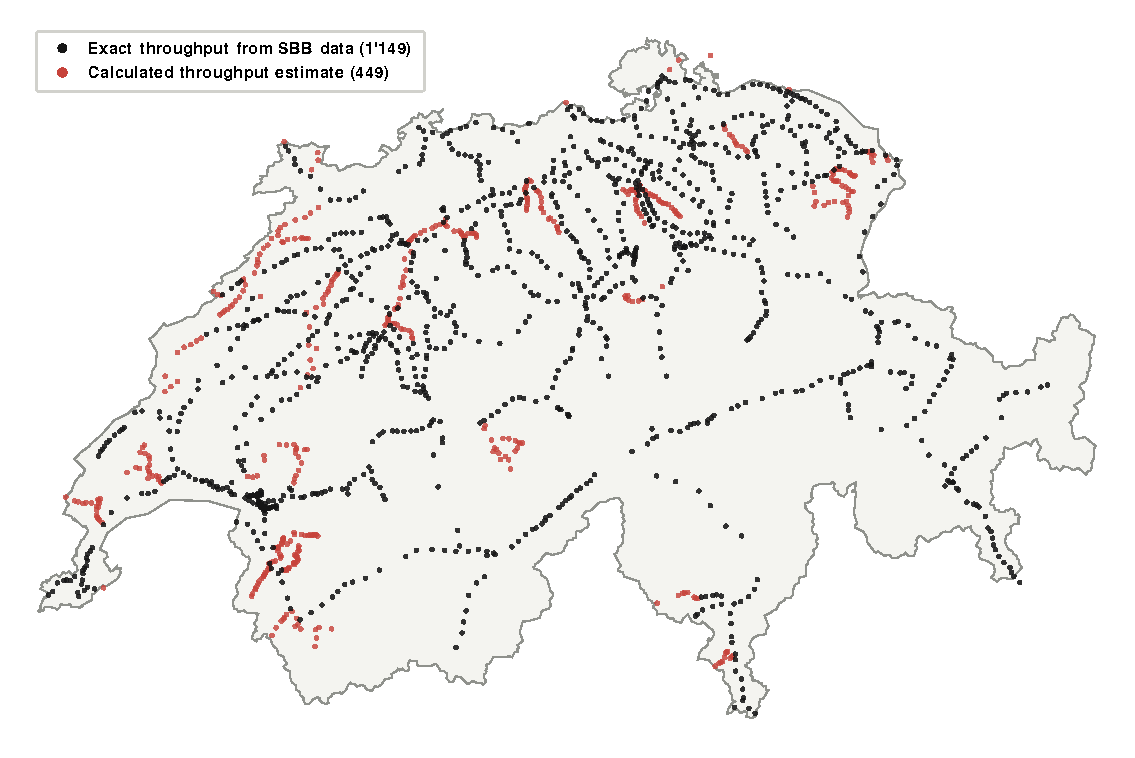
\includegraphics[width=0.70\textwidth]{figures/part-II/sbb_station_frequency_coverage_map.pdf}
\caption[Part II station map of throughput data coverage]{Part II's station set, coloured by whether station throughput was sourced or calculated.}
\label{fig:part2-sbb-throughput-coverage}
\end{figure}


Let \(S_y\) denote the year-specific station set for \(y\in\{2026,2035\}\), and let \(T_i^y\) denote the daily station-throughput target for station \(i\in S_y\). Station throughput is defined as the total number of passenger movements involving the station, whether as an origin, destination, or intermediate transfer point. Where exact station matches are available, official SBB passenger-frequency data are used as the preferred source for these targets \citep{sbbPassagierfrequenzDataset2026}. The Part~II timetable, however, is larger than the coverage of this dataset and includes minor, narrow-gauge, and future stations for which no directly usable SBB DTV (Durchschnittlicher Tagesverkehr, average daily traffic volume) observation could be assigned. In the station metadata, 1'149 of the 1'598 total stations were matched exactly to SBB passenger-frequency observations. The remaining 449 station rows were assigned model-estimated fallback values. Figure~\ref{fig:part2-sbb-throughput-coverage} shows the spatial distribution of exact SBB throughput values and calculated throughput estimates in the Part~II station set.

For unmatched stations, the retained fallback model is a log-linear OLS specification fitted only on the exactly matched stations. The model estimates
\begin{equation}
\begin{aligned}
\log\left(1+\frac{\widehat T_i}{1\ \mathrm{pax/day}}\right)
={}&
\beta_0
+\beta_P\log\left(1+\frac{P_i}{1\ \mathrm{pax}}\right)
+\beta_L\log\left(1+\frac{L_i}{1\ \mathrm{line}}\right)\\
&+\beta_{PL}
\log\left(1+\frac{P_i}{1\ \mathrm{pax}}\right)
\log\left(1+\frac{L_i}{1\ \mathrm{line}}\right).
\end{aligned}
\label{eq:part2-dtv-fallback}
\end{equation}

with fitted coefficients

\begin{equation}
(\beta_0,\beta_P,\beta_L,\beta_{PL})
=
(-1.795817,\ 0.691244,\ 3.936396,\ -0.197348).
\label{eq:part2-dtv-fallback-coefficients}
\end{equation}

Here, \(\widehat T_i\) is the fallback DTV estimate, \(P_i\) is the mean of the 2026 and 2035 distributed station-population values, and \(L_i\) is the corresponding mean number of line services. The source value assigned to station \(i\) is therefore

\begin{equation}
T_i^{\mathrm{source}}
=
\begin{cases}
T_i^{\mathrm{SBB}}, & \text{if station } i \text{ has an exact SBB passenger-frequency match},\\[4pt]
\widehat T_i, & \text{otherwise}.
\end{cases}
\label{eq:part2-dtv-source-assignment}
\end{equation}

The fitted fallback model achieves \(R^2=0.7681\) on the log scale and \(R^2=0.4756\) on the raw passenger scale. It therefore captures the approximate order-of-magnitude relationship between station population, service intensity, and observed station frequency, but it is not precise enough to replace observed counts at individual high-flow stations. This limitation is acceptable because exact SBB observations are retained wherever available, while fitted values are used only to provide plausible throughput constraints for otherwise unmatched stations before the subsequent transfer correction and IPF balancing steps. Figure~\ref{fig:part2-sbb-throughput-coverage} indicates that stations without SBB throughput data are concentrated on comparatively simple line systems with few overlapping services. Their estimates are therefore less likely to materially alter the optimization-relevant demand structure at higher-flow, centrally located transfer stations.


\subsubsection{Pre-balancing OD demand matrix}\label{sec:methods-part2-demand-seed}
The pre-balancing OD matrix defines the relative pattern of station-to-station demand before the station-throughput constraints are imposed. Its role is to provide a plausible starting distribution for the later balancing step: larger and better-served stations should attract more trips, while pairs with long distances, low frequency, long waits, and poor transfer conditions should receive less demand. The final IPF procedure in Chapter~\ref{sec:methods-part2-demand-balancing} then preserves this relative OD structure as far as possible while forcing the matrix to match the corrected station-throughput targets. For an ordered station pair \((i,j)\), the pre-balancing OD value is

\begin{equation}
\widetilde M^y_{ij}
=
\lambda^y
\exp\left(O_i^y+D_j^y+U_{ij}^y\right),
\qquad
\widetilde M^y_{ii}=0,
\label{eq:part2-gravity-seed}
\end{equation}

where \(\lambda^y\) is a scale factor used to put the raw gravity matrix on the observed station-throughput scale before balancing. The origin and destination attractiveness terms are

\begin{equation}
\begin{aligned}
O_i^y
={}&
a_P\log\left(1+\frac{P_i^y}{1\ \mathrm{pax}}\right)
+
a_L\log\left(1+\frac{L_i^y}{1\ \mathrm{line}}\right),\\
D_j^y
={}&
b_P\log\left(1+\frac{P_j^y}{1\ \mathrm{pax}}\right)
+
b_L\log\left(1+\frac{L_j^y}{1\ \mathrm{line}}\right).
\end{aligned}
\label{eq:part2-origin-destination-terms}
\end{equation}

where \(P_i^y\) is the distributed station population and \(L_i^y\) is the number of line services at station \(i\) in year \(y\). The remaining term \(U_{ij}^y\) is the OD-pair impedance and service term: it adjusts the provisional demand between \(i\) and \(j\) according to the timetable quality and spatial separation of that specific station pair.

\begin{equation}
\begin{aligned}
U_{ij}^y={}&
\gamma_f\log\left(1+\frac{f_{ij}^y}{1\ \mathrm{service/day}}\right)
-\gamma_d\log\left(1+\frac{d_{ij}}{1\ \mathrm{km}}\right)\\
&-\gamma_a\frac{a_{ij}^y}{1\ \mathrm{min}}
-\gamma_w\frac{w_{ij}^y}{1\ \mathrm{min}}
-\gamma_r\frac{r_{ij}^y}{1\ \mathrm{min}}
-\gamma_h\frac{h_{ij}^y}{1\ \mathrm{min}}
-\gamma_q\frac{q_{ij}^y}{1\ \mathrm{min}} .
\end{aligned}
\label{eq:part2-gravity-pair-utility}
\end{equation}

Here, \(f_{ij}^y\) is the OD service-frequency proxy, \(d_{ij}\) is the crow-fly station distance, \(a_{ij}^y\) is the fastest observed after-boarding connection time, and \(w_{ij}^y\) is the initial waiting-time value from the routing skim. Following the path-component convention introduced in Section~\ref{sec:data-path-representation} and illustrated in Figure~\ref{fig:path-representation-example}, \(r_{ij}^y\), \(h_{ij}^y\), and \(q_{ij}^y\) denote the rolling, same-train dwell, and transfer-time components of the OD routes. Thus, frequency and station attractiveness increase the provisional OD value, while distance and timetable impedance reduce it. The calibration also includes a small hub-throughput adjustment when comparing a candidate matrix with observed SBB station-frequency values. For a candidate matrix, the raw station-throughput proxy is

\begin{equation}
\widehat T_i^{y,\mathrm{raw}}
=
\left(1+\gamma_g H_i^y\right)
\left(
\sum_{j\ne i}\widetilde M^y_{ij}
+
\sum_{j\ne i}\widetilde M^y_{ji}
\right),
\label{eq:part2-gravity-throughput-proxy}
\end{equation}

where \(H_i^y\) is the line-service count of station \(i\), rescaled to the interval \([0,1]\) within the model year. The coefficient \(\gamma_g\) controls the strength of the hub-throughput multiplier \((1+\gamma_g H_i^y)\). This multiplier allows the calibration to raise predicted throughput slightly at high-service stations, where station-frequency observations typically includes more transfer-related activity not explainable by population and OD-pair impedance alone. The hub term is used only in the calibration-side station-throughput comparison and does not add demand to any specific OD pair.

The 2026 calibration uses a random search over candidate parameter vectors. 2'000 alternative coefficient sets are drawn from bounded parameter ranges. Each coefficient set is used to construct a complete gravity matrix, convert it to station-throughput predictions, scale it analytically to the exact SBB-matched stations, and score it against the year-aligned SBB station-throughput observations. This search strategy is used because the calibration target is nonlinear in the coefficients and is evaluated after exponentiation, zero-diagonal OD construction, station-throughput aggregation, and scaling.

The retained 2026 coefficient values are

\begin{equation}
\begin{array}{llll}
 a_P=0.583612, & a_L=1.035827, & b_P=0.442745, & b_L=1.024021,\\
 \gamma_f=0.153353, & \gamma_d=0.318544, & \gamma_a=0.023483, & \gamma_w=0.025076,\\
 \gamma_r=0.013692, & \gamma_h=0.026526, & \gamma_q=0.143372, & \gamma_g=0.000736.
\end{array}
\label{eq:part2-gravity-coefficients}
\end{equation}

The best 2026 pre-balancing candidate was evaluated against 1'149 exact SBB validation stations. Before marginal balancing, it achieved \(R^2=0.4143\), a mean absolute error (MAE) of \(2'292.49\), a root mean squared error (RMSE) of \(13'137.42\), and a mean absolute percentage error (MAPE) of \(67.22\%\) against year-aligned station throughput. These values indicate that the gravity model is not a precise station-throughput predictor on its own. This is acceptable here because the gravity model is used to shape the relative OD pattern before IPF, while the final station totals are imposed through the corrected throughput targets in Section~\ref{sec:methods-part2-demand-balancing}.

The 2035 pre-balancing matrix reuses the coefficients calibrated on the 2026 matrix, but replaces the station attributes and route skims with their 2035 values. This keeps the behavioural weighting rule fixed while allowing the future timetable, population distribution, and service pattern to change the provisional OD structure. A small accessibility adjustment is also applied to the 2035 station-throughput targets before final balancing, so that stations with improved 2035 connectivity can receive a modest increase in target throughput.

For station \(s\), the accessibility index is computed by first evaluating the calibrated OD-pair utility \(U_{sj}^y\) from station \(s\) to every other station \(j\) in year \(y\). This utility uses the same service and impedance terms as the pre-balancing gravity matrix: frequency enters positively, while distance, fastest after-boarding time, initial waiting time, rolling time, dwell time, and transfer time enter negatively. The exponential \(\exp(U_{sj}^y)\) converts each destination relation into a positive accessibility contribution. A destination with frequent, fast, and low-transfer service from \(s\) therefore contributes more than a destination that is distant or poorly connected. These destination contributions are then summed:

\begin{equation}
A_s^y=\sum_{j\ne s}\exp\left(U_{sj}^y\right),
\qquad
\Delta\ln A_s=\ln A_s^{2035}-\ln A_s^{2026}.
\label{eq:part2-accessibility-change}
\end{equation}

\(A_s^y\) is a gravity-based accessibility score derived from scanning the routing of station pairs. The logarithmic change \(\Delta\ln A_s\) measures whether station \(s\) becomes better or worse connected in the 2035 timetable under the same calibrated utility weights.

The unbounded accessibility factor is

\begin{equation}
\widetilde u_s
=
\sqrt{
\exp\left(\eta_o\Delta\ln A_s\right)
\exp\left(\eta_d\Delta\ln A_s\right)
}
=
\exp\left(\frac{\eta_o+\eta_d}{2}\Delta\ln A_s\right).
\label{eq:part2-2035-accessibility-factor-raw}
\end{equation}

The factor applied to the 2035 station target is then bounded:

\begin{equation}
u_s
=
\min\left\{1.80,\max\left\{0.70,\widetilde u_s\right\}\right\},
\qquad
T_s^{2035,\mathrm{adj}}
=
T_s^{2035,\mathrm{pop/service}}u_s.
\label{eq:part2-2035-induced-demand}
\end{equation}

The retained elasticities are \(\eta_o=\eta_d=0.25\). The square-root form combines the origin-side and destination-side accessibility responses into one station-throughput factor, because the subsequent balancing step uses a single throughput target per station rather than separate production and attraction targets. The bounds \([0.70,1.80]\) are a modelling safeguard that prevent the accessibility adjustment alone from reducing a station target below 70\% or increasing it above 180\%.

Before the transfer-throughput correction, the resulting 2035 network uplift factor is 1.0186. Thus, the accessibility adjustment raises the aggregate 2035 station target by about 1.86\%. The effect is small, but lets the 2035 service pattern affect the demand weights without turning the optimization comparison into a large induced-demand scenario, which is out of scope of this thesis' line of research.

\subsubsection{Demand correction and balancing}\label{sec:methods-part2-demand-balancing}
The gravity-shaped OD matrix still requires two corrections before the final station-constrained matrix is accepted. The first concerns the unmatched stations identified in Section~\ref{sec:methods-part2-demand-throughput}. For these stations, the fallback DTV estimate is treated as uncertain rather than as a fully observed marginal constraint, so the target is adjusted toward the raw station throughput implied by the gravity model. Exact SBB-matched stations remain unchanged.

Let \(T_i^{y,\mathrm{pre}}\) be the station-throughput target before this correction, and let \(G_i^y\) be the raw gravity-implied station throughput before marginal balancing. For 2026, the corrected target after the unmatched-station adjustment is

\begin{equation}
\bar T_i^{2026}
=
\begin{cases}
T_i^{2026,\mathrm{SBB}}, & i\ \text{has an exact SBB match},\\[4pt]
\left(T_i^{2026,\mathrm{pre}}\right)^\alpha
\left(G_i^{2026}\right)^{1-\alpha}, & i\ \text{has no exact SBB match},
\end{cases}
\label{eq:part2-unmatched-target-blend}
\end{equation}

with \(\alpha=0.5\). For unmatched stations, this is the geometric mean of the pre-correction target and the raw gravity-implied throughput. The geometric form is used because station throughputs vary over several orders of magnitude; it adjusts uncertain fallback targets proportionally rather than by an absolute additive amount. For 2035, the same idea is applied while preserving the previously constructed 2035 uplift for stations that also exist in the 2026 station set:

\begin{equation}
\bar T_i^{2035}
=
\begin{cases}
T_i^{2035,\mathrm{SBB}}, & i\ \text{has an exact SBB match},\\[4pt]
\bar T_i^{2026}
\dfrac{T_i^{2035,\mathrm{pre}}}{T_i^{2026,\mathrm{pre}}},
& i\ \text{has no exact SBB match and exists in both years},\\[10pt]
\left(T_i^{2035,\mathrm{pre}}\right)^\alpha
\left(G_i^{2035}\right)^{1-\alpha},
& i\ \text{has no exact SBB match and exists only in 2035}.
\end{cases}
\label{eq:part2-unmatched-target-2035}
\end{equation}

Thus, exact SBB stations retain their year-aligned observed throughput values. Unmatched 2026 stations are shrunk toward the raw gravity throughput. Unmatched 2035 stations normally inherit the station-specific 2035/2026 uplift from the original target construction, applied to the corrected 2026 target; only 2035-only stations use the direct geometric blend.

The second correction accounts for transfer double-counting in the SBB station-frequency definition introduced above. Let \(B_i^y\) be the daily transfer-passenger proxy at station \(i\), calculated from allocated transfer paths. Since one transferring passenger contributes one alighting and one boarding in the SBB frequency convention, the transfer proxy enters as \(2B_i^y\). The transfer-corrected target is

\begin{equation}
T_i^{y,\mathrm{corr}}
=
\max\left(
\phi\bar T_i^y,
\bar T_i^y\left[
1-
\min\left(
\kappa,
\rho\frac{2B_i^y}{\bar T_i^y}
\right)
\right]
\right),
\label{eq:part2-transfer-target-correction}
\end{equation}

where \(\rho=0.4\), \(\kappa=0.7\), and \(\phi=0.3\). The parameter \(\rho\) controls how strongly estimated transfer passengers reduce the station-throughput target, \(\kappa\) caps the maximum transfer discount at 70\%, and \(\phi\) ensures that the corrected target cannot fall below 30\% of the pre-discount value. The correction therefore reduces clear transfer double-counting at hubs.

A short-distance urban damping rule is also applied to the OD matrix used as the starting point for the final balancing. This reduces selected short OD cells in the starting matrix, before the row and column totals are forced to match the station-throughput targets. The purpose is to prevent dense urban station pairs around line-rich nodes from dominating the matrix purely because several nearby stations lie close together. Let \(\omega_{ij}^y\) be the damping factor:

\begin{equation}
\omega_{ij}^y
=
\begin{cases}
0.25+0.75\left(\dfrac{d_{ij}}{12\ \mathrm{km}}\right)^{0.75},
& 0<d_{ij}<12\ \mathrm{km}\ \text{and}\ \max(L_i^y,L_j^y)\ge 8,\\[8pt]
1,
& \text{otherwise}.
\end{cases}
\label{eq:part2-short-urban-damping}
\end{equation}

Here, \(d_{ij}\) is the crow-fly distance in kilometres and \(L_i^y\) is the line-service count at station \(i\). The damped starting matrix for the final balancing is

\begin{equation}
M_{ij}^{y,(0)}=\omega_{ij}^y M_{ij}^{y,\mathrm{grav}},
\qquad
M_{ii}^{y,(0)}=0,
\label{eq:part2-damped-starting-matrix}
\end{equation}

where \(M^{y,\mathrm{grav}}\) is the gravity-shaped OD matrix entering the final correction stage. The rule affected 4'422 OD cells in 2026 and 5'766 OD cells in 2035, with mean damping factors of 0.7457 and 0.7527 respectively. The final OD matrices are then obtained by iterative proportional fitting. Since \(T_i^{y,\mathrm{corr}}\) is a station-throughput target, each OD trip contributes once at the origin and once at the destination. The row and column targets are therefore set symmetrically:

\begin{equation}
R_i^y=C_i^y=\frac{T_i^{y,\mathrm{corr}}}{2}.
\label{eq:part2-row-column-targets}
\end{equation}

Starting from \(M^{y,(0)}\), the same iterative proportional fitting row-column scaling logic as in Equation~\eqref{eq:historical-ipf} is applied with row targets \(R_i^y\) and column targets \(C_i^y\), while preserving the zero diagonal:

\begin{equation}
M^y
=
\operatorname{IPF}_{M_{ii}=0}\left(M^{y,(0)};R^y,C^y\right).
\label{eq:part2-final-ipf}
\end{equation}

The final 2026 transfer-discounted target total is 4'063'399.63 station-throughput passengers per day, corresponding to 2'031'699.82 directed OD passengers per day before route-comparison station-scope filtering. The final 2035 target total is 4'329'812.43, corresponding to 2'164'906.22 directed OD passengers per day before filtering. The final IPF runs converged with maximum relative row errors of \(4.85\times10^{-9}\) in 2026 and \(5.83\times10^{-9}\) in 2035; the corresponding column errors were below \(10^{-14}\) in both years.

\subsection{Timetable/path layer}\label{sec:methods-part2-paths}
The Part~II timetable/path layer converts each year--scenario timetable into retained station-to-station path alternatives. It uses the same compact timetable-token convention, event-graph structure, lexicographic route search, and dominance-minute weighting introduced in Data Preparation and Methods~I. In Part~II these operations are repeated for Baseline and Optimized Steps~1--3. The output is a full station-level path set for each year and scenario, which is then joined with the fixed OD matrix from the demand layer.


Let \(\sigma\in\{0,1,2,3\}\) denote the scenario, with \(\sigma=0\) for the baseline and \(\sigma=1,2,3\) for Steps~1--3. The corresponding timetable state in year \(y\) is denoted by \(T^{y,\sigma}\). In this section, an \emph{event} means a single arrival or departure instance obtained after converting the compact periodic timetable tokens into clock times. A transfer event is a feasible pairing between one arrival event and a later departure event, subject to the relevant station-specific minimum transfer time.

\subsubsection{Periodic timetable expansion}\label{sec:methods-part2-periodic-expansion}
The parser uses the compact timetable-token structure defined in Equation~\eqref{eq:data-token}. As a reminder, each active timetable cell is represented by a minute value \(m\), a frequency mode \(\mu\), and the continuation flags \(P\) and \(Q\). The admissible hour set \(H(\tau)\) is the same as in Equation~\eqref{eq:allowed-hours}: suffixless tokens are hourly, \(n\)-tokens use even hours, and \(i\)-tokens use odd hours. The \(P\) and \(Q\) flags follow the continuation logic introduced in Section~\ref{sec:logic} and formalized for Part~I in Equation~\eqref{eq:continuation-bound}. Part~II applies this same token parser to the 2026 and 2035 baseline and optimized scenario columns.

Let \(\nu\) index consecutive arrival/departure rows within one train-run chain. For row \(\nu\), let
\[
\tau_\nu=(m_\nu,\mu_\nu,P_\nu,Q_\nu)
\]
be the parsed token. Here, \(m_\nu\) is the minute within the hour, \(\mu_\nu\) determines the admissible hour set, and \(P_\nu\) and \(Q_\nu\) are the continuation flags. The possible clock-time occurrences of this token, measured in minutes after midnight, are

\begin{equation}
O(\tau_\nu)=\{60h+m_\nu:h\in H(\tau_\nu)\},
\label{eq:part2-occurrence-set}
\end{equation}

where \(h\) is the clock-hour index. Departure events are retained for \(300\le t<1440\), corresponding to departures from 05:00 until before midnight. Concrete event times are selected from \(O(\tau_\nu)\) with the same next-occurrence rule used in Part~I, given in Equations~\eqref{eq:next-event-time}--\eqref{eq:continuation-bound}. Part~II keeps the same \(P/Q\) continuation semantics. Same-station arrival--departure continuations are retained as same-train dwell only up to the implemented through-dwell limit of 15 minutes; longer waits are treated as a new line service. This rule is to facilitate the automatic identification of out-and-back services' implied terminal stations.
\newpage
\subsubsection{Event-graph routing}\label{sec:methods-part2-event-graph-search}
For each year \(y\) and scenario \(\sigma\), the parsed timetable state \(T^{y,\sigma}\) is represented as a directed event graph \(G(T^{y,\sigma})\). As in the Part~I event graph in Equation~\eqref{eq:historical-event-graph}, \(G\) consists of event nodes \(V\) and directed edge sets \(E\) that represent feasible passenger actions:

\begin{equation}
G(T^{y,\sigma})=
\left(
V^{y,\sigma},
E^{\mathrm{run},y,\sigma}
\cup
E^{\mathrm{wait},y,\sigma}
\cup
E^{\mathrm{transfer},y,\sigma}
\right).
\label{eq:part2-scenario-graph}
\end{equation}

Here, \(V^{y,\sigma}\) is the set of concrete timetable events in year \(y\) and scenario \(\sigma\). Each event stores its station, clock time, service identity, and whether it is an arrival or departure. The edge sets \(E^{\mathrm{run},y,\sigma}\), \(E^{\mathrm{wait},y,\sigma}\), and \(E^{\mathrm{transfer},y,\sigma}\) contain run, wait, and transfer edges respectively. Run edges connect consecutive events on the same train run. Wait edges connect later departure events at the same station. Transfer edges connect an arrival event to a feasible later departure event on another train. This is the same passenger-action structure as in Chapter~\ref{sec:methods-part1-eventgraph}; but in Part~II, the graph is reconstructed for each optimized timetable state.

OD path search follows the lexicographic route label introduced in Equation~\eqref{eq:lexicographic-label}. For a query from origin \(i\) to destination \(j\) at query minute \(q\), the router first minimizes arrival time, then prefers the latest possible first departure among equally early arrivals, then minimizes transfers, and finally minimizes movement segments. The retained alternatives for an OD pair are the distinct paths selected over the representative two-hour query window, following the dominance-cache logic of Chapter~\ref{sec:methods-part1-cache}.

Minimum-transfer feasibility is enforced while building transfer edges. Let \(\mathcal{A}^{y,\sigma}\subset V^{y,\sigma}\) be the set of arrival events and \(\mathcal{D}^{y,\sigma}\subset V^{y,\sigma}\) the set of departure events. For an arrival event \(a\in\mathcal{A}^{y,\sigma}\) and a departure event \(d\in\mathcal{D}^{y,\sigma}\), let \(s(a)\) and \(s(d)\) be their station nodes, \(t(a)\) and \(t(d)\) their event times in minutes after midnight, and \(\operatorname{run}(a)\), \(\operatorname{run}(d)\) their train-run identities. The transfer interval between the two events is

\begin{equation}
\Delta t_{a,d}=t(d)-t(a).
\label{eq:part2-transfer-wait}
\end{equation}

A transfer edge is created exactly when the event pair represents a change to a different train run and the required minimum transfer time is met:

\begin{equation}
(a,d)\in E^{\mathrm{transfer},y,\sigma}
\Longleftrightarrow
\begin{cases}
a\in\mathcal{A}^{y,\sigma},\quad d\in\mathcal{D}^{y,\sigma},\\
\operatorname{run}(a)\ne\operatorname{run}(d),\\
\Delta t_{a,d}\ge m(s(a),s(d)).
\end{cases}
\label{eq:part2-transfer-edge-rule}
\end{equation}

The pairwise minimum transfer time \(m(s,s')\) is the shared station-transfer rule defined in Equation~\eqref{eq:data-transfer-time-rule}. For ordinary stations, that rule permits transfers only within the same station node using the station-specific minimum transfer time \(m_s\). For Zürich HB, it permits transfers within the station-alias complex using the 4-minute rule for Zürich HB (31--34) self-transfers and the 7-minute rule for other Zürich HB alias combinations. Cases with \(m(s,s')=\infty\) cannot satisfy Equation~\eqref{eq:part2-transfer-edge-rule}, so no transfer edge is created.

The route builder prevents minimum-transfer violations caused by the interaction of same-train dwell edges and departure-to-departure wait edges. A passenger may remain on the same train through a dwell stop, but a subsequent switch to another train is allowed only if the minimum transfer time from the original arrival has elapsed.

\subsubsection{Path allocation}\label{sec:methods-part2-path-allocation}
For each OD pair \((i,j)\), year \(y\), and scenario \(\sigma\), the route builder stores a retained path set \(\mathcal{P}_{ij}^{y,\sigma}\). These are the nondominated path alternatives selected by the lexicographic route search over the representative two-hour query window, following the dominance-cache principle introduced in Chapter~\ref{sec:methods-part1-cache}. Each path \(p\in\mathcal{P}_{ij}^{y,\sigma}\) stores its first departure minute \(\operatorname{dep}_p^{y,\sigma}\), arrival minute \(\operatorname{arr}_p^{y,\sigma}\), rolling time \(r_p^{y,\sigma}\), same-train dwell time \(h_p^{y,\sigma}\), and transfer time \(q_p^{y,\sigma}\). All times are measured in minutes.
The total post-departure travel time path cost is

\begin{equation}
c_p^{y,\sigma}
=
r_p^{y,\sigma}
+
h_p^{y,\sigma}
+
q_p^{y,\sigma}.
\label{eq:part2-path-cost}
\end{equation}

This uses the same rolling--dwell--transfer decomposition introduced in Chapter~\ref{sec:data-path-representation} and used for Part~I in Equation~\ref{eq:part1-total-time-components}. Same-minute intermediate stops are treated with the 20-second dwell time convention described in Chapter~\ref{sec:data-path-representation}; the component totals are then rebalanced so that \(c_p^{y,\sigma}\) remains equal to the elapsed after-boarding time \(\operatorname{arr}_p^{y,\sigma}-\operatorname{dep}_p^{y,\sigma}\). Initial waiting is stored separately because it occurs before first boarding and is not part of the post-departure optimization objective.

The fixed OD demand \(M_{ij}^y\) is allocated across the retained path alternatives by dominance minutes. Let \(C=120\ \mathrm{min}\) be the clockface cycle length. For path \(p\), the valid daily departure instances are


\begin{equation}
\mathcal{I}_p^{y,\sigma}
=
\left\{
\operatorname{dep}_p^{y,\sigma}+nC:
n\in\mathbb{Z}_{\ge0},\,
300\le \operatorname{dep}_p^{y,\sigma}+nC<1440,\,
\operatorname{dep}_p^{y,\sigma}+nC+c_p^{y,\sigma}<1440
\right\}.
\label{eq:part2-daily-repetitions}
\end{equation}

Here, \(n\) counts repetitions of the two-hour pattern during the service day. The first time bound keeps departures between 05:00 and midnight. The final condition excludes repeated path instances whose arrival would fall at or after midnight.

For OD pair \((i,j)\), collect all valid departure instances from all saved paths and sort them by time:

\begin{equation}
\mathcal{U}_{ij}^{y,\sigma}
=
\left\{
(u,p):p\in\mathcal{P}_{ij}^{y,\sigma},\ u\in\mathcal{I}_p^{y,\sigma}
\right\}.
\label{eq:part2-valid-departure-instances}
\end{equation}

Write the sorted departure times as
\(u_1<u_2<\cdots<u_{N_{ij}^{y,\sigma}}\), where \(N_{ij}^{y,\sigma}\) is the number of valid departure instances for OD pair \((i,j)\). Let \(p(u_\xi)\) denote the saved path associated with departure instance \(u_\xi\). The value \(u_0=300\) is used to start the 05:00 service-day. The service-day dominance minutes assigned to path \(p\) are therefore

\begin{equation}
\beta_p^{y,\sigma}
=
\sum_{\xi:\,p(u_\xi)=p}
\left(u_\xi-u_{\xi-1}\right).
\label{eq:part2-dominance-minutes}
\end{equation}

For a simple example, in the 2008 IC~1 row of Table~\ref{tab:token-expansion}, the Bern--Zürich HB service departs Bern at minute :32 each hour. If this were the saved path for an OD pair, the first valid departure after the 05:00 start would be \(u_1=332\), i.e. 05:32. It would receive \(332-300=32\) dominance minutes. The next departure, \(u_2=392\), i.e. 06:32, would receive \(392-332=60\) dominance minutes. The same logic is applied to all saved path alternatives in the OD cell.

Thus, each valid departure receives the interval of service-day minutes immediately preceding it. This is the same dominance-minute idea as Equation~\eqref{eq:part1-dominance-minutes} and Figure~\ref{fig:dominance-cache-example}, applied here to all saved path alternatives. The path share \(\alpha_p^{y,\sigma}\) is obtained by normalizing the dominance minutes of path \(p\) over all retained path alternatives for the same OD pair, year, and scenario:

\begin{equation}
\alpha_p^{y,\sigma}
=
\frac{\beta_p^{y,\sigma}}
{\sum_{p'\in\mathcal{P}_{ij}^{y,\sigma}}\beta_{p'}^{y,\sigma}}.
\label{eq:part2-path-share}
\end{equation}

Here, \(p'\) is a summation index over the retained path set \(\mathcal{P}_{ij}^{y,\sigma}\), and \(\beta_{p'}^{y,\sigma}\) is the service-day dominance-minute count of path \(p'\). Thus, \(\alpha_p^{y,\sigma}\) is the fraction of the OD demand for pair \((i,j)\) assigned to path \(p\). If the denominator is zero in an exceptional cell, the implementation assigns equal shares across the valid retained paths. Otherwise, Equation~\eqref{eq:part2-path-share} determines the complete path allocation.

The allocated daily passenger flow on path \(p\) is

\begin{equation}
x_p^{y,\sigma}
=
M_{ij}^y\alpha_p^{y,\sigma}.
\label{eq:part2-path-demand}
\end{equation}

Here, \(M_{ij}^y\) is the fixed daily OD demand from station \(i\) to station \(j\) in year \(y\), measured in passengers per day, and \(x_p^{y,\sigma}\) is the corresponding daily passenger flow assigned to path \(p\). Importantly, the OD demand matrix \(M^y\) is fixed across Baseline and Steps~1--3 within the same year. Scenario differences therefore come only from retimed events, changed route choices, and changed dominance shares. For path-level diagnostic summaries, the allocation also stores the number of valid daily departure instances of each path:

\begin{equation}
n_p^{y,\sigma}
=
\left|\mathcal{I}_p^{y,\sigma}\right|.
\label{eq:part2-path-instance-count}
\end{equation}

Here, \(\mathcal{I}_p^{y,\sigma}\) is the set of valid daily departure instances of path \(p\), defined in Equation~\eqref{eq:part2-daily-repetitions}. Since the path-allocation table stores the total dominance minutes \(\beta_p^{y,\sigma}\) and the number of valid instances \(n_p^{y,\sigma}\), the diagnostic path-level initial wait \(\widehat w_p^{y,\sigma}\) is computed as one half of the mean assigned interval:

\begin{equation}
\widehat w_p^{y,\sigma}
=
\frac{\beta_p^{y,\sigma}}{2n_p^{y,\sigma}}.
\label{eq:part2-random-arrival-wait}
\end{equation}

\(\widehat w_p^{y,\sigma}\) is a path-level diagnostic derived from the stored dominance allocation fields, and is not part of the optimization objective. The corresponding wait-inclusive diagnostic cost is

\begin{equation}
(c_p^+)^{y,\sigma}
=
c_p^{y,\sigma}
+
\widehat w_p^{y,\sigma}.
\label{eq:part2-wait-inclusive-path-cost}
\end{equation}

The optimization and validation results use \(c_p^{y,\sigma}\), the post-departure cost after boarding. The wait-inclusive value \((c_p^+)^{y,\sigma}\) is reported separately to isolate the effect of path dominance and departure spacing on the overall cost.

\subsection{Optimization layer}\label{sec:methods-part2-optimization}
The optimization layer corresponds to Steps~9--12 in Figure~\ref{fig:part2-workflow}. It receives the fixed year-specific OD matrix from the demand layer and the saved path alternatives from the timetable/path layer. Its task is to identify small integer-minute retimings that reduce passenger-weighted post-departure travel time while preserving the structure of the periodic timetable. The search is local by design: it does not redesign the timetable from scratch, but tests feasible line-section shifts generated from high-flow transfer and near-miss contexts.

The layer is organized in four parts. First, the common passenger-minute objective used for final validation is defined. Second, the shared physical edit type is introduced: local integer-minute section shifts that preserve rolling time, together with the transfer and near-miss effects used to generate and screen those shifts. Third, the restricted binary candidate-selection problem is formulated using optimization terminology. Fourth, the three selection steps are separated: Step~1 is driven mainly by station-board transfer and near-miss evidence, Step~2 scores additional candidates against exact Step~1 reference paths, and Step~3 broadens and repeatedly re-scores the search from the completed Step~2 timetable.

\subsubsection{Validation objective}\label{sec:methods-part2-optimization-objective}
Let \(y\in\{2026,2035\}\) denote the model year. Let \(\sigma\in\{0,1,2,3\}\) denote the timetable scenario, where \(\sigma=0\) is the baseline and \(\sigma=1,2,3\) are the completed Step~1, Step~2, and Step~3 timetables. The corresponding timetable state is denoted by \(T^{y,\sigma}\). The OD demand matrix \(M^y\) is fixed within each year, so \(M^y_{ij}\) [pax/day] is identical across all four scenarios. Unless stated otherwise, sums over OD pairs are taken over active directed station pairs with \(M^y_{ij}>0\).

For any complete timetable state \(T\), define the validation objective \(F^y(T)\) as the total daily post-departure passenger-minutes obtained after rebuilding all OD paths:

\begin{equation}
  F^y(T)
  =
  \sum_{(i,j)}
  M^y_{ij}
  \sum_{p\in\mathcal{P}_{ij}^{y}(T)}
  \alpha_p^y(T)c_p^y(T).
  \label{eq:part2-validation-objective-intro}
\end{equation}

Here, \(\mathcal{P}_{ij}^{y}(T)\) is the retained nondominated path set for OD pair \((i,j)\) under timetable \(T\), following the route-search construction in Section~\ref{sec:methods-part2-event-graph-search}. The path share \(\alpha_p^y(T)\) corresponds to the dominance-minute share defined in Equation~\eqref{eq:part2-path-share}, and \(c_p^y(T)\) [min] is the post-departure cost after boarding defined in Equation~\eqref{eq:part2-path-cost}. Since \(M^y_{ij}\) is measured in passengers per day and \(c_p^y(T)\) in minutes, \(F^y(T)\) is measured in passenger-minutes per day.

Conceptually, the passenger-time objective is

\[
  \min_{T\in\mathcal{T}_y} F^y(T),
\]

where \(\mathcal{T}_y\) is the set of feasible timetable states for year \(y\). A global timetable-optimization model would search directly over this feasible set. In the Part~II setting, however, the value of \(F^y(T)\) is only known after the route builder has been run for a complete timetable state. A one-minute retiming can change transfer waits, retained path alternatives, and the dominance-minute allocation of OD demand across those alternatives.

As discussed in Section~\ref{sec:periodic-timetabling}, decomposition has extended the scale of microscopic timetable planning, while integrated models with endogenous passenger routing have been demonstrated on much smaller station networks. The two fully-built timetable years in Part~II each contain nearly 1'600 stations and roughly 2.5 million directed OD pairs. A global formulation combining periodic timetable variables, transfer constraints, passenger-path decisions, and dominance-minute allocation would therefore far exceed the station and OD coverage established by the reviewed passenger-oriented models. Benders or another decomposition method could improve manageability, but the literature does not establish that the complete formulation used here would be solvable to a useful bound at national scale.

The strategy applied here keeps the passenger-flow perspective of an integrated model, but avoids solving the entire network as one exact optimization problem. It identifies high-impact local timetable alterations from passenger-flow evidence, then validates the completed scenarios through a full OD path rebuild. Feasible local section shifts are generated and selected with restricted binary candidate-selection proxies, as formalized in Sections~\ref{sec:methods-part2-transfer-context-candidates}--\ref{sec:methods-part2-step2-search}. Each completed scenario is then evaluated by rebuilding all OD paths under the validation objective \(F^y(T)\), with the scenario-comparison metrics defined in Section~\ref{sec:methods-part2-analysis}.

Using the path-allocation notation from Section~\ref{sec:methods-part2-path-allocation}, the same objective for scenario \(\sigma\) can be written as

\begin{equation}
F^{y,\sigma}
=
F^y(T^{y,\sigma})
=
\sum_{(i,j)}
\sum_{p\in\mathcal{P}_{ij}^{y,\sigma}}
x_p^{y,\sigma}c_p^{y,\sigma}
=
\sum_{(i,j)}
\sum_{p\in\mathcal{P}_{ij}^{y,\sigma}}
x_p^{y,\sigma}
\left(
r_p^{y,\sigma}+h_p^{y,\sigma}+q_p^{y,\sigma}
\right).
\label{eq:part2-full-objective}
\end{equation}

Here, \(x_p^{y,\sigma}\) [pax/day] is the daily passenger flow allocated to path \(p\), and \(r_p^{y,\sigma}\), \(h_p^{y,\sigma}\), and \(q_p^{y,\sigma}\) [min] are the rolling, same-train dwell, and transfer components defined in Section~\ref{sec:data-path-representation}.

The objective can also be read at station-pair level. For an active OD pair \((i,j)\), the representative post-departure time of one modelled trip is

\begin{equation}
\bar c_{ij}^{y,\sigma}
=
\sum_{p\in\mathcal{P}_{ij}^{y,\sigma}}
\alpha_p^{y,\sigma}c_p^{y,\sigma}
=
\frac{1}{M_{ij}^y}
\sum_{p\in\mathcal{P}_{ij}^{y,\sigma}}
x_p^{y,\sigma}c_p^{y,\sigma}.
\label{eq:part2-od-mean-cost}
\end{equation}

Here, \(\bar c_{ij}^{y,\sigma}\) [min/trip] is the dominance-weighted post-departure travel time for a representative trip from station \(i\) to station \(j\) in scenario \(\sigma\). The corresponding daily passenger-minute contribution of this OD pair is

\begin{equation}
F_{ij}^{y,\sigma}
=
M_{ij}^y\bar c_{ij}^{y,\sigma}
=
\sum_{p\in\mathcal{P}_{ij}^{y,\sigma}}
x_p^{y,\sigma}c_p^{y,\sigma}.
\label{eq:part2-od-passenger-minute-contribution}
\end{equation}
\newpage
The OD-level change against the baseline is

\begin{equation}
\Delta \bar c_{ij}^{y,\sigma}
=
\bar c_{ij}^{y,\sigma}
-
\bar c_{ij}^{y,0},
\qquad
\Delta F_{ij}^{y,\sigma}
=
F_{ij}^{y,\sigma}
-
F_{ij}^{y,0}
=
M_{ij}^y\Delta \bar c_{ij}^{y,\sigma}.
\label{eq:part2-od-delta}
\end{equation}

A station pair improves if \(\Delta \bar c_{ij}^{y,\sigma}<0\), worsens if \(\Delta \bar c_{ij}^{y,\sigma}>0\), and is unchanged if \(\Delta \bar c_{ij}^{y,\sigma}=0\). The first value measures the change for a representative trip on that OD pair, while the second value measures its daily passenger-minute importance. Thus, a one-minute improvement on a high-demand OD pair contributes more to the national objective than the same one-minute improvement on a lightly used pair.

The scenario change against the baseline is the sum of these OD-level contributions:

\begin{equation}
\Delta F^{y,\sigma}
=
F^{y,\sigma}-F^{y,0}
=
\sum_{(i,j)}
\Delta F_{ij}^{y,\sigma}
=
\sum_{(i,j)}
M_{ij}^y\Delta \bar c_{ij}^{y,\sigma}.
\label{eq:part2-scenario-delta}
\end{equation}

A negative value of \(\Delta F^{y,\sigma}\) means that the retimed scenario reduces total daily post-departure passenger-minutes. Initial waiting time is reported separately as a diagnostic, because it occurs before first boarding and is not part of the optimization objective.

\subsubsection{Transfer context and retiming candidates}\label{sec:methods-part2-transfer-context-candidates}
The transfer context links the path-allocation layer to the retiming search. For existing transfers, routed path demand is aggregated into line-to-line transfer patterns at each station. A transfer-context row therefore represents passengers who arrive on one service and continue on another service at the same transfer location, weighted by the daily path flow assigned to that transfer. High-flow transfer rows are then expanded into repeated service-day occurrences using the same 120-minute periodicity as the path-allocation layer. In parallel, the station-board construction compares feasible arrivals and departures at each station and identifies near-miss opportunities, meaning arrival--departure pairs that are close to, but do not yet satisfy, the station-specific minimum transfer time.

A timetable retiming candidate is a line-section shift,

\begin{equation}
z=(y,\ell,u,v,\bar d_z,\bar a_z,\delta_z),
\label{eq:part2-candidate-shift}
\end{equation}

where \(y\) is the model year, \(\ell\) is the affected line, \(u\rightarrow v\) is the directed line section from upstream station \(u\) to downstream station \(v\), and \(\delta_z\) [min] is the proposed integer-minute offset. The search is intended to be minimally disruptive to the overall network: candidate shifts are therefore restricted to

\begin{equation}
\delta_z\in\Delta,
\qquad
\Delta=\{-10,-9,\ldots,-1,1,\ldots,10\}.
\label{eq:part2-shift-domain}
\end{equation}

Thus, a retiming candidate may move the affected section by at most 10 minutes earlier or later, while the zero-shift case is excluded because it would leave the timetable unchanged. This bound is applied relative to the timetable state being searched: Step~1 starts from \(T^{y,0}\), Step~2 from \(T^{y,1}\), and Step~3 from \(T^{y,2}\). The values \(\bar d_z\) and \(\bar a_z\) identify the departure and arrival positions of this section within the representative two-hour pattern. They are included because the same line and directed section may occur more than once within the clockface cycle.

Applying candidate \(z\) shifts the section departure at \(u\) and the corresponding section arrival at \(v\) by the same number of minutes:

\begin{equation}
t'_{\ell,u,\mathrm{dep}}
=
t_{\ell,u,\mathrm{dep}}+\delta_z,
\qquad
t'_{\ell,v,\mathrm{arr}}
=
t_{\ell,v,\mathrm{arr}}+\delta_z.
\label{eq:part2-section-shift}
\end{equation}

Here, \(t_{\ell,u,\mathrm{dep}}\) and \(t_{\ell,v,\mathrm{arr}}\) [min] are the original section departure and arrival times for the affected pattern occurrence, and primes denote the retimed values. The same shift is applied to the corresponding service-day repetitions of that clockface section. Since both endpoints of the section move by the same offset, the section rolling time is unchanged:

\begin{equation}
\left(
t'_{\ell,v,\mathrm{arr}}
-
t'_{\ell,u,\mathrm{dep}}
\right)
-
\left(
t_{\ell,v,\mathrm{arr}}
-
t_{\ell,u,\mathrm{dep}}
\right)
=0.
\label{eq:part2-rolling-invariant}
\end{equation}

This rolling-time invariant is a hard constraint, as this thesis aims to find only timetable improvements that do not require altering the travel time between neighboring stations on the same line. A validated timetable edit may therefore improve or worsen transfer waiting time, and it may consume or release available dwell leeway around the shifted section, but it may not make the train itself move any faster along that section. The timetable validator also checks to ensure legitimate periodic tokens, preserved \(i/n\) and \(P/Q\) suffix semantics as introduced in Chapter~\ref{sec:logic}, unaltered line station order and arrival/departure sequence, persistent section rolling durations, sufficient same-train dwell leeway, and acceptable through-dwell bounds.

For a transfer occurrence \(\omega\), let \(g_\omega\) [min] be the scheduled interval between the arrival of the incoming service and the departure of the onward service before any retiming is applied. Let \(m_\omega\) [min] be the minimum transfer time required for that arrival--departure pair. Let \(X_\omega\) [pax/day] denote the daily passenger weight used when scoring this occurrence. For an existing feasible transfer, this weight comes directly from the path-allocation layer: it is the daily passenger flow on retained paths that currently use the transfer. For a near miss, no passengers are yet routed through the connection because the transfer is infeasible. Its weight is therefore estimated from each station's arrival/departure boards by asking how much passenger flow could plausibly benefit if the arrival--departure pair became feasible, based on the demand attached to the relevant incoming and onward services at that station. If candidate \(z\) changes the incoming arrival by \(\Delta_\omega^{\mathrm{arr}}(z)\) [min] and the onward departure by \(\Delta_\omega^{\mathrm{dep}}(z)\) [min], the shifted transfer wait is

\begin{equation}
g'_\omega(z)
=
g_\omega
+
\Delta_\omega^{\mathrm{dep}}(z)
-
\Delta_\omega^{\mathrm{arr}}(z).
\label{eq:part2-shifted-wait}
\end{equation}

A positive value of \(\Delta_\omega^{\mathrm{dep}}(z)\) means that the onward departure is moved later, while a positive value of \(\Delta_\omega^{\mathrm{arr}}(z)\) means that the incoming arrival is moved later. Thus, a later departure increases the transfer wait, whereas a later arrival reduces it.

For the existing-transfer safeguard, a high-flow transfer is defined as follows. Let \(\Omega\) denote an aggregated line-to-line transfer, and let \(X_\Omega\) [pax/day] be the daily path demand assigned to that transfer pattern. A transfer is classified as high-flow if

\begin{equation}
X_\Omega \ge X^{\min},
\qquad
X^{\min}=95\ \text{pax/day}.
\label{eq:part2-high-flow-transfer-threshold}
\end{equation}

This corresponds to roughly five passengers per operating hour over the 05:00--23:59 service day. Each high-flow row \(\Omega\) is then expanded into repeated transfer occurrences \(\omega\) in the two-hour clockface pattern. The occurrence \(\omega\) inherits the daily passenger weight \(X_\omega=X_\Omega\), which is used when scoring candidate retimings.

Let \(\mathcal{E}_z\) be the set of existing high-flow transfer occurrences affected by candidate \(z\). An occurrence is affected when \(z\) changes either its incoming arrival time or its onward departure time. For each occurrence \(\omega\in\mathcal{E}_z\), the scheduled arrival-to-departure interval before applying \(z\) is denoted by \(g_\omega\) [min]. The corresponding interval after applying \(z\) is denoted by \(g'_\omega(z)\) [min]. The required minimum transfer time is \(m_\omega\) [min]. The daily passenger weight attached to the underlying transfer row is \(X_\omega\) [pax/day].

For each existing transfer occurrence that remains feasible after candidate \(z\), the occurrence-level transfer gain \(G_\omega(z)\) is

\begin{equation}
G_\omega(z)
=
X_\omega
\left(
g_\omega-g'_\omega(z)
\right),
\qquad
g_\omega\ge m_\omega,\quad
g'_\omega(z)\ge m_\omega.
\label{eq:part2-existing-transfer-gain}
\end{equation}

Here, \(G_\omega(z)\) [pax\(\cdot\)min/day] is positive when candidate \(z\) shortens this specific transfer occurrence, and negative when it lengthens the occurrence while keeping it feasible. It is not yet the total score of candidate \(z\). Candidate-level scores combine affected transfer, near-miss, and reference-path evidence according to the step-specific rules below.

If an existing high-flow transfer falls below the minimum transfer time after the timetable shift, the candidate is considered to have broken that transfer. The set of broken high-flow transfer occurrences is

\begin{equation}
\mathcal{B}_z
=
\left\{
\omega\in\mathcal{E}_z:
g_\omega\ge m_\omega
\ \text{and}\
g'_\omega(z)<m_\omega
\right\}.
\label{eq:part2-broken-transfer-set}
\end{equation}

The associated broken-transfer passenger flow is

\begin{equation}
B_z
=
\sum_{\omega\in\mathcal{B}_z}
X_\omega .
\label{eq:part2-broken-transfer-flow}
\end{equation}

Here, \(B_z\) [pax/day] is the daily passenger flow attached to high-flow transfers that candidate \(z\) would make infeasible. In Step~1, retained candidates require \(\mathcal{B}_z=\emptyset\), equivalently \(B_z=0\). Steps~2 and~3 add path-based safeguards: candidates are rejected if they invalidate any affected retained reference path carrying passenger flow, as defined in Sections~\ref{sec:methods-part2-step2-search} and~\ref{sec:methods-part2-step3-search}.

For a currently infeasible near-miss occurrence \(\eta\), let \(g_\eta\) [min] be the current arrival-to-departure interval. The required minimum transfer time is \(m_\eta\) [min], and the potential passenger weight assigned from the station-board context is \(X_\eta\) [pax/day]. The current minimum-transfer shortfall is

\begin{equation}
s_\eta
=
\max(0,m_\eta-g_\eta).
\label{eq:part2-near-miss-shortfall}
\end{equation}

After applying candidate \(z\), the shifted interval \(g'_\eta(z)\) is computed with the same rule as in Equation~\eqref{eq:part2-shifted-wait}. The remaining shortfall is

\begin{equation}
s'_\eta(z)
=
\max(0,m_\eta-g'_\eta(z)).
\label{eq:part2-shifted-near-miss-shortfall}
\end{equation}

The occurrence-level near-miss gain is then

\begin{equation}
G_\eta^{\mathrm{miss}}(z)
=
X_\eta
\left[
s_\eta-s'_\eta(z)
\right].
\label{eq:part2-near-miss-gain}
\end{equation}

Here, \(G_\eta^{\mathrm{miss}}(z)\) [pax\(\cdot\)min/day] is the weighted reduction in minimum-transfer shortfall caused by candidate \(z\). If \(s'_\eta(z)=0\), the arrival--departure pair becomes a newly feasible transfer. If \(s'_\eta(z)>0\), the candidate reduces the shortfall but does not yet create a usable connection. All three steps use these reductions as screening evidence, with different weights, because they indicate retimings that move local transfer structure in a favourable direction. In the final validation and analysis, realized transfer improvements are counted only when passengers can actually use the resulting connection: either if an existing feasible transfer is shortened, or a near miss crosses the minimum-transfer threshold and becomes feasible.


\subsubsection{Candidate scoring and selection}\label{sec:methods-part2-candidate-proxy}
This subsection defines the common scoring and selection structure used by all three optimization steps. Each step starts from a finite list of feasible retiming candidates, where each candidate has an associated step-specific passenger-minute score and undergoes compatibility checks. The Steps~1-3 rules then differ in how these candidates are scored, filtered, and accepted.

For optimization step \(s\in\{1,2,3\}\) and year \(y\), let \(\mathcal{C}^{(s)}_y\) be the candidate set generated for that step. Candidates are evaluated from the completed timetable produced by the preceding step: \(T^{y,0}\) for Step~1, \(T^{y,1}\) for Step~2, and \(T^{y,2}\) for Step~3. For each candidate \(z\in\mathcal{C}^{(s)}_y\), define the binary selection variable

\[
x^{(s)}_z=
\begin{cases}
1, & \text{if candidate }z\text{ is selected},\\
0, & \text{otherwise}.
\end{cases}
\]

Once each candidate has been scored and checked for feasibility and conflicts, the remaining task is to choose which candidates to apply. Written in binary decision-variable form, this selection problem is

\begin{equation}
\begin{aligned}
  \max_{x^{(s)}}\quad
  & \sum_{z\in\mathcal{C}^{(s)}_y}
    \widehat G^{(s)}_z x^{(s)}_z \\
  \text{s.t.}\quad
  & A^{(s)}x^{(s)}\le \mathbf{1},\\
  & x^{(s)}_z=0
    \qquad \forall z\notin\mathcal{V}^{(s)}(T^{y,s-1}),\\
  & \Gamma^{(s)}x^{(s)}\le \gamma^{(s)},\\
  & x^{(s)}_z\in\{0,1\}
    \qquad \forall z\in\mathcal{C}^{(s)}_y .
\end{aligned}
\label{eq:part2-restricted-ip-proxy}
\end{equation}

The coefficient \(\widehat G^{(s)}_z\) [pax\(\cdot\)min/day] is the passenger-minute saving score assigned to candidate \(z\) in Step \(s\). The proxy problem is written as a maximization: larger values indicate larger expected reductions in post-departure time, even though the final validation objective \(F^y(T)\) in Equation~\eqref{eq:part2-validation-objective-intro} is minimized. In Step~1, \(\widehat G^{(1)}_z\) is based on station-board existing-transfer and near-miss evidence, as defined in Equation~\eqref{eq:part2-step1-proxy-intro}. In Step~2, \(\widehat G^{(2)}_z\) is based on the exact cost change of affected paths retained under Step~1, with the complete score defined in Equations~\eqref{eq:part2-step2-exact-saving}--\eqref{eq:part2-step2-score}. In Step~3, the analogous coefficient is iteration-dependent: \(S_z^{(3,a)}\) in Equation~\eqref{eq:part2-step3-score} combines the marginal saving on Step~2 reference paths with conservatively weighted near-miss evidence and is recomputed after each accepted addition.

The matrix \(A^{(s)}\) describes mutually incompatible candidates. Each row of \(A^{(s)}\) corresponds to one incompatibility group, such as candidates that touch the same timetable event key or would apply inconsistent edits to the same local timetable structure. The vector \(\mathbf{1}\) is a vector of ones with one entry per incompatibility group. Thus, \(A^{(s)}x^{(s)}\le\mathbf{1}\) means that at most one candidate from each incompatibility group can be selected.

The set \(\mathcal{V}^{(s)}(T^{y,s-1})\) contains candidates that pass the step-specific timetable validator when tested against the timetable state at the start of step \(s\). The validator checks the structural conditions introduced in Section~\ref{sec:methods-part2-transfer-context-candidates}: legitimate periodic tokens, preserved \(i/n\) and \(P/Q\) semantics, unchanged line station order and arrival/departure sequence, unchanged section rolling times, sufficient dwell and leeway bounds, and the relevant transfer-safety rules for the step. 

The constraint \(\Gamma^{(s)}x^{(s)}\le\gamma^{(s)}\) represents step-specific search-budget restrictions rather than timetable feasibility. Step~1 has no accepted-edit cap. Step~2 permits at most 20 new additions across both years after its hub filtering and exact reference-path evaluation; 19 additions were ultimately retained. Step~3 again has no fixed accepted-edit cap, instead using the minimum score and compatibility conditions in Equation~\eqref{eq:part2-step3-acceptance-rule}.


Equation~\eqref{eq:part2-restricted-ip-proxy} shows how the candidate-selection problem would look if all candidate scores and feasibility checks were treated as fixed inputs. In that form, it is a 0--1 linear integer program: each candidate is either selected or not selected, and the objective is linear in those binary choices. The implemented selector follows the same logic, but applies it sequentially. Candidates are considered in ranked order; when a candidate is accepted, it is immediately applied to the working timetable before the next candidate is checked.

Let \(z_1,z_2,\ldots,z_J\) be the ranked candidate list for a given step and year, where \(J=|\mathcal{C}^{(s)}_y|\). Let \(\mathcal{A}^{(s)}_r\) be the set of candidates accepted after the first \(r\) candidates have been considered, with \(\mathcal{A}^{(s)}_0=\emptyset\). Let \(T^{(s)}_r\) be the corresponding working timetable after those decisions, with \(T^{(1)}_0=T^{y,0}\), \(T^{(2)}_0=T^{y,1}\), and \(T^{(3)}_0=T^{y,2}\). Finally, let \(\Phi^{(s)}(z_r,\mathcal{A}^{(s)}_r,T^{(s)}_r)\) be the step-specific acceptance check. This check is true only if candidate \(z_r\) has a sufficient score, is compatible with the already accepted candidates, respects any applicable search budget, and passes the timetable validator on the current working timetable.


The cumulative selection rule is

\begin{equation}
\mathcal{A}^{(s)}_{r+1}
=
\begin{cases}
\mathcal{A}^{(s)}_r\cup\{z_r\},
& \Phi^{(s)}(z_r,\mathcal{A}^{(s)}_r,T^{(s)}_r)=1,\\[4pt]
\mathcal{A}^{(s)}_r,
& \Phi^{(s)}(z_r,\mathcal{A}^{(s)}_r,T^{(s)}_r)=0,
\end{cases}
\label{eq:part2-cumulative-selection}
\end{equation}

with the working timetable updated as

\begin{equation}
T^{(s)}_{r+1}
=
\begin{cases}
T^{(s)}_r\oplus z_r,
& \Phi^{(s)}(z_r,\mathcal{A}^{(s)}_r,T^{(s)}_r)=1,\\[4pt]
T^{(s)}_r,
& \Phi^{(s)}(z_r,\mathcal{A}^{(s)}_r,T^{(s)}_r)=0.
\end{cases}
\label{eq:part2-working-timetable-update}
\end{equation}

Here, \(T^{(s)}_r\oplus z_r\) denotes the timetable obtained by applying candidate \(z_r\) to the current working timetable. After all \(J\) candidates have been considered, the accepted set is \(\mathcal{A}^{(s)}_J\). For later notation, this accepted set is converted back into binary form:

\begin{equation}
\widehat{x}^{(s)}_z
=
\begin{cases}
1, & \text{if candidate }z\text{ is in the accepted set }\mathcal{A}^{(s)}_J,\\
0, & \text{otherwise}.
\end{cases}
\label{eq:part2-selected-vector}
\end{equation}

Thus, \(\widehat{x}^{(s)}\) records the candidates selected by the sequential procedure after the ranked list has been processed. It is the output of the implemented acceptance rule and is not a global maximizer of the binary proxy problem in Equation~\eqref{eq:part2-restricted-ip-proxy}. The step-specific checks are defined in Sections~\ref{sec:methods-part2-step1-selection}--\ref{sec:methods-part2-step3-search}.

When compared to algorithmic periodic timetable-optimization, a full periodic event-scheduling problem (PESP) or MILP timetable model would represent event times directly as optimization variables. For an activity \(e=(i,j)\), such as a run, dwell, headway, or transfer activity, a standard PESP-style timing constraint has the form

\begin{equation}
L_e
\le
\pi_j-\pi_i+\Pi n_e
\le
U_e,
\qquad
n_e\in\mathbb{Z}.
\label{eq:part2-reference-pesp-constraint}
\end{equation}

Here, \(\pi_i\) and \(\pi_j\) [min] are periodic event times, \(\Pi\) [min] is the timetable period, \(n_e\) is an integer wrap variable, and \(L_e\) and \(U_e\) [min] are the lower and upper bounds for activity \(e\). In such a formulation, event times, wrap variables, and activity constraints are optimized jointly. In this thesis, corresponding types of timetable-feasibility requirements are enforced through candidate generation and timetable validation processes, while passenger effects are evaluated through the full OD path rebuild. The final timetable improvement is therefore able to be measured by the validated change in Equation~\eqref{eq:part2-validation-objective-intro} after rebuilding the timetable, instead of by the proxy scores alone.

\subsubsection{Step~1 missed-transfer candidate selection}\label{sec:methods-part2-step1-selection}
Step~1 is the first of three steps that identify promising timetable edits. It starts from the baseline timetable \(T^{y,0}\) and uses station-board transfer evidence to identify local missed-transfer edits before the full OD validation layer rebuilds paths. The existing-transfer input is restricted to high-flow transfer rows, using the threshold in Equation~\eqref{eq:part2-high-flow-transfer-threshold}. With \(X^{\min}=95\) [pax/day], this corresponds to transfers being considered that are used by at least five passengers per operating hour over the 05:00--23:59 operating day. Each retained transfer row is expanded into repeated transfer occurrences using the 120-minute periodicity described in the path-allocation layer. The near-miss input comes from station-board arrival--departure pairs that are infeasible in the Baseline scenario because they fall below the required minimum transfer time, but that could become feasible after a local section retiming within the shift domain \(\Delta\) defined in Equation~\eqref{eq:part2-shift-domain}.

The Step~1 candidate field is focused on missed-transfer retimings. A timetable edit is retained only if it reduces the minimum-transfer shortfall of at least one near-miss occurrence, where the shortfall is defined in Equation~\eqref{eq:part2-near-miss-shortfall}. This can occur either by shifting the arrival-side section earlier or by shifting the departure-side section later. Because the same physical section shift also changes the timing of the line segment at its other endpoint, the Step~1 score includes both the intended near-miss improvement and any resulting local transfer side effects. Candidates then pass through the station-board selection filters before full OD path validation: the current proxy score must be positive, at least one near-miss occurrence must be improved, no retained high-flow existing transfer may be broken, and no timetable-safety or feasibility flag may be triggered.
\paragraph*{Station-board score.}
For a candidate \(z\) evaluated against a current working timetable \(T\), let \(T+z\) denote the timetable that would result from applying candidate \(z\) to \(T\). Let \(\mathcal{E}_z(T)\) be the set of existing high-flow transfers in the current timetable \(T\) for which candidate \(z\) changes either the incoming arrival time or the onward departure time, and which remain feasible after applying \(z\). Let \(\mathcal{N}_z(T)\) be the set of near-miss occurrences in the current timetable \(T\) for which candidate \(z\) changes either the incoming arrival time or the onward departure time. The Step~1 passenger-minute saving proxy \(\widehat G_z^{(1)}(T)\) is

\begin{equation}
\widehat G_z^{(1)}(T)
=
\sum_{\omega\in\mathcal{E}_z(T)}
X_\omega
\left[
g_\omega(T)-g_\omega(T+z)
\right]
+
\sum_{\eta\in\mathcal{N}_z(T)}
X_\eta
\left[
s_\eta(T)-s_\eta(T+z)
\right].
\label{eq:part2-step1-proxy-intro}
\end{equation}

Here, \(g_\omega(T)\) [min] is the scheduled arrival--departure interval of existing transfer occurrence \(\omega\) in timetable \(T\), and \(g_\omega(T+z)\) [min] is the corresponding interval after applying candidate \(z\). The term \(s_\eta(T)\) [min] is the minimum-transfer shortfall of near-miss occurrence \(\eta\) in timetable \(T\), as defined in Equation~\eqref{eq:part2-near-miss-shortfall}; \(s_\eta(T+z)\) [min] is the remaining shortfall after applying the candidate. The weights \(X_\omega\) and \(X_\eta\) [pax/day] are the occurrence-level passenger weights described in Section~\ref{sec:methods-part2-transfer-context-candidates}. The first sum measures the weighted effect of shortened or lengthened existing transfers that remain feasible. The second sum measures the weighted reduction in near-miss shortfalls. Thus \(\widehat G_z^{(1)}(T)\) is a local estimate of the candidate's passenger-minute effect, measured in passenger-minutes per day. Because accepted edits are applied immediately, this score is re-evaluated against the current working timetable rather than only against the original baseline.
\paragraph*{Acceptance rule.}
Step~1 is intended to find edits that help missed transfers, so the selector requires each accepted candidate to reduce the shortfall of at least one near-miss occurrence in the current timetable. Let

\begin{equation}
\mathcal{N}^{+}_z(T)
=
\left\{
\eta\in\mathcal{N}_z(T):
s_\eta(T+z)<s_\eta(T)
\right\},
\qquad
P^{\mathrm{miss}}_z(T)
=
\sum_{\eta\in\mathcal{N}^{+}_z(T)}X_\eta .
\label{eq:part2-step1-near-miss-flow}
\end{equation}

Here, \(T+z\) is the timetable obtained by applying candidate \(z\) to the current timetable \(T\). The set \(\mathcal{N}^{+}_z(T)\) contains the near-miss occurrences whose minimum-transfer shortfall is smaller after the edit than before it. The value \(P^{\mathrm{miss}}_z(T)\) [pax/day] is the corresponding station-board potential-flow weight. A positive value means that the candidate improves at least one near-miss occurrence, although the occurrence does not necessarily become fully feasible.

The Step~1 acceptance rule is written as

\begin{equation}
\Phi^{(1)}(z,T)=1
\Longleftrightarrow
\begin{cases}
\widehat G_z^{(1)}(T)>0,\\
P^{\mathrm{miss}}_z(T)>0,\\
B_z(T)=0,\\
V(z,T)=1.
\end{cases}
\label{eq:part2-step1-greedy}
\end{equation}

Here, \(\Phi^{(1)}(z,T)=1\) means that candidate \(z\) is accepted by the Step~1 station-board selector when tested against timetable \(T\). The first condition requires a positive current passenger-minute saving estimate. The second condition keeps the search focused on missed-transfer improvements. The third condition rejects candidates that would make any retained high-flow existing transfer infeasible, where \(B_z(T)\) [pax/day] is the broken high-flow transfer flow from Equation~\eqref{eq:part2-broken-transfer-flow}. The fourth condition requires the structural timetable validator to accept the edit; \(V(z,T)=1\) means that the physical shift satisfies the token, sequence, rolling-time, dwell, and leeway checks introduced in Section~\ref{sec:methods-part2-transfer-context-candidates}.

If all four conditions hold, the edit is accepted and immediately applied before the next candidate is tested. Unlike Step~2, Step~1 uses no fixed edit acceptance cap and stops only when a full pass accepts no additional candidate.
\paragraph*{Validated Step~1 timetable.}
The station-board selector produced 31 proposed Step~1 timetable edits: 9 for 2026 and 22 for 2035. These proposed edits were not yet the final Step~1 scenario. They were passed to the full OD validation layer, where the path set was rebuilt and compared with the baseline. The Step~1 scenario retained only edits whose validation status showed lower passenger-weighted total post-departure time for the attributed OD paths. This totalled 18 accepted Step~1 timetable edits: 7 for 2026 and 11 for 2035. The completed Step~1 timetable therefore altered a doubled total of 36 arrival/departure times: 14 in 2026 and 22 in 2035.

For year \(y\), the validated Step~1 timetable \(T^{y,1}\) is

\begin{equation}
T^{y,1}
=
T^{y,0}
\oplus
z^{(1)}_{1,y}
\oplus
z^{(1)}_{2,y}
\oplus
\cdots
\oplus
z^{(1)}_{K_y^{(1)},y},
\label{eq:part2-step1-timetable}
\end{equation}

where \(T^{y,0}\) is the baseline timetable, \(z^{(1)}_{1,y},\ldots,z^{(1)}_{K_y^{(1)},y}\) are the retained Step~1 timetable edits for year \(y\), and \(K_y^{(1)}\) is the number of retained Step~1 rows in that year. The operator~\(\oplus\) denotes sequential application of these edits to the timetable state: after each accepted section shift is applied, the next edit is interpreted against the updated timetable. These validated Step~1 edits form the starting timetable for the subsequent Step~2 candidate search.


\subsubsection{Step~2 reference-path candidate selection}\label{sec:methods-part2-step2-search}

Step~2 starts from the validated Step~1 timetable \(T^{y,1}\). Unlike Step~1, it is not primarily a missed-transfer search; it evaluates additional potential timetable edits against the exact reference paths selected under \(T^{y,1}\), while retaining near-miss evidence only as a discounted secondary signal. A candidate can therefore become attractive in Step~2 even if it was not retained in Step~1, because the Step~1 edits may have changed path dominance, changed which line sections are used by retained paths, or created cumulative interactions across several nearby connections.
\paragraph*{Hub filter.}
Before the exact reference-path scan, Step~2 applies a hub filter to keep the search concentrated around stations where local retiming is most likely to matter. This filter does not define independent timetable subproblems. It simply marks station-year pairs whose neighbouring candidate shifts should remain eligible for Step~2. The filtered candidates are then evaluated together in one shared Step~2 selection pool, with the compatibility checks in Equation~\eqref{eq:part2-step2-acceptance-rule}.

Let \(h\) denote a transfer station. For each station-year pair \((h,y)\), define \(R_{h,y}\) [pax/day] as the daily passenger flow on existing routed transfers at station \(h\), and \(U_{h,y}\) [pax/day] as the daily potential passenger flow on near-miss transfers at station \(h\). The Step~2 hub score is

\begin{equation}
S^{\mathrm{hub}}_{h,y}
=
R_{h,y}
+
10U_{h,y}.
\label{eq:part2-step2-hub-score}
\end{equation}

The multiplier 10 is dimensionless. It gives additional priority to near-miss potential, so that stations with many almost-feasible transfers are not hidden by stations with larger already-routed transfer volumes. Within each year, stations are ranked in descending order of \(S^{\mathrm{hub}}_{h,y}\). Here, \(\operatorname{rank}_y(\cdot)\) is the descending within-year rank, with rank 1 assigned to the highest-scoring station in year \(y\). The retained hub-filter set is

\begin{equation}
\begin{aligned}
\mathcal{H}
=
\{(h,y):\;&
\operatorname{rank}_y(S^{\mathrm{hub}}_{h,y})\le 28\\
&\lor\ U_{h,y}\ge 500\ \mathrm{pax/day}\\
&\lor\ h\in\mathcal{M}_{\mathrm{main}}
\}.
\end{aligned}
\label{eq:part2-step2-hub-scope}
\end{equation}

In the above equation, \(\mathcal{M}_{\mathrm{main}}\) is a manual list of 23 nationally important interchange stations. It is included so that major interchange locations remain eligible for Step~2 even if their local near-miss score is lower in one model year. In this thesis' implementation, the top-28 score rule selected 28 stations in each year. The near-miss threshold then added 56 further station-year pairs in 2026 and 50 in 2035. The fixed main-hub safeguard added 2 further pairs in 2026 and 6 in 2035. The final hub-filter set therefore contained 170 station-year pairs in total: 86 in 2026 and 84 in 2035.
\paragraph*{Candidate table and preliminary filtering.}
The hub filter is then applied to the proposed timetable edit table. This table is built from the same physical section-shift representation introduced in Equation~\eqref{eq:part2-candidate-shift}. Starting from the Step~1 timetable \(T^{y,1}\), the candidate generator enumerates line-section shifts with \(\delta_z\in\Delta\), where \(\Delta\) is the \(\pm10\)-minute shift domain defined in Equation~\eqref{eq:part2-shift-domain}. For each candidate, the table stores the fields needed to identify and pre-screen the edit: the affected line, the shifted section \(u\rightarrow v\), the section's departure and arrival positions in the two-hour pattern, the proposed shift \(\delta_z\), the transfer stations touched by the edit, and the local dwell/leeway margins that determine whether the shift can be absorbed without changing section rolling times. It also stores the station-board transfer effects introduced in Section~\ref{sec:methods-part2-transfer-context-candidates}: passenger-minute gains from shortened feasible transfers, passenger-minute gains from reduced near-miss shortfalls, passenger-minute losses from worsened feasible transfers, and any broken-transfer flags. The retained Step~1 timetable edits are removed from this table so that Step~2 only considers additional edits. Let \(\mathcal{C}^{\mathrm{phys}}_y\) denote this table of newly proposed physical section shifts for year \(y\). Each row is a candidate \(z\) with the structure defined in Equation~\eqref{eq:part2-candidate-shift}. Let \(\mathcal{H}_y=\{h:(h,y)\in\mathcal{H}\}\) be the retained hub-filter stations in year \(y\). Let \(\mathcal{S}_z\) be the set of stations associated with candidate \(z\), consisting of its shifted section endpoints and the transfer stations touched by its station-board effects. Before the exact reference-path scan, Step~2 applies a first filter based on local station-board evidence and structural feasibility:

\begin{equation}
\begin{aligned}
\mathcal{C}^{(2)}_y
=
\{z\in\mathcal{C}^{\mathrm{phys}}_y:\;&
P^{\mathrm{net}}_z\ge50\ \mathrm{pax{\cdot}min/day},\\
&
P^{\mathrm{gain}}_z\ge200\ \mathrm{pax{\cdot}min/day},\\
&
P^{\mathrm{loss}}_z/P^{\mathrm{gain}}_z\le0.75,\\
&
B_z=0,\\
&
\psi_z=1,\\
&
\mathcal{S}_z\cap\mathcal{H}_y\ne\emptyset
\}.
\end{aligned}
\label{eq:part2-step2-static-filter}
\end{equation}

Here, \(P^{\mathrm{gain}}_z\), \(P^{\mathrm{loss}}_z\), and \(P^{\mathrm{net}}_z\) [pax\(\cdot\)min/day] are preliminary passenger-minute estimates computed from the station-board transfer effects in Section~\ref{sec:methods-part2-transfer-context-candidates}, before the more detailed reference-path scan is run. \(P^{\mathrm{gain}}_z\) is the gross local improvement from shortened feasible transfers and reduced near-miss shortfalls, \(P^{\mathrm{loss}}_z\) is the gross local worsening from lengthened feasible transfers, and \(P^{\mathrm{net}}_z=P^{\mathrm{gain}}_z-P^{\mathrm{loss}}_z\) is the corresponding net station-board effect. The thresholds \(P^{\mathrm{net}}_z\ge50\) and \(P^{\mathrm{gain}}_z\ge200\) keep the exact reference-path scan limited to candidates with a relevantly-sized local benefit signal. The loss-ratio condition \(P^{\mathrm{loss}}_z/P^{\mathrm{gain}}_z\le0.75\) excludes candidates whose local transfer harm is large relative to their local gain; equivalently, the station-board gross loss must not exceed 75\% of the gross gain. This keeps ambiguous high-side-effect candidates out of the expensive path scan while still allowing candidates with some local worsening.

The condition \(B_z=0\) uses the broken-transfer flow from Equation~\eqref{eq:part2-broken-transfer-flow} and excludes candidates that would make a protected existing transfer infeasible. The remaining structural flag \(\psi_z=1\) excludes candidates with same-line transfer pairs or knock-on effects at neighbouring stops. The flag is raised when the proposed section shift cannot be cleanly bounded using available same-train dwell margins: such candidates must be excluded because the edit would propagate to neighbouring sections instead of remaining local. In the implemented run, the filters that most strongly reduced the candidate table were the broken-transfer safeguard, which removed 5'236 rows; the same-line transfer-pair exclusion, which removed 3'874 rows; and the neighbouring-station knock-on-effect exclusion, which removed 1'957 rows. The local-benefit thresholds removed a further 794 rows for insufficient gross gain and 211 rows for insufficient net gain, while the hub filter removed 123 rows. Only 2 rows were removed by the 0.75 loss-ratio condition. Candidates passing these filters were ranked by \(P^{\mathrm{net}}_z\), then by \(P^{\mathrm{gain}}_z\) and \(P^{\mathrm{loss}}_z\). To keep the exact reference-path scan computationally manageable, Step~2 sends only the 450 highest-ranked filtered rows to the next stage. These rows form the candidate set that is evaluated against the Step~1 reference paths.
\paragraph*{Reference-path evaluation.}
For each candidate \(z\) in this reduced set, Step~2 scans the exact Step~1 reference paths. Let \(\mathcal{R}^{y,1}_z\) be the set of Step~1 paths that traverse the physical line section affected by \(z\). These are reference paths, not newly rerouted paths: they are the paths already selected under \(T^{y,1}\). For each path \(p\in\mathcal{R}^{y,1}_z\), let

\[
\chi_{p,z}
=
\begin{cases}
1, & \text{if path \(p\) remains transfer-feasible after applying candidate \(z\),}\\
0, & \text{otherwise.}
\end{cases}
\]

The exact reference-path saving \(E_z\) is

\begin{equation}
E_z
=
\sum_{p\in\mathcal{R}^{y,1}_z}
\chi_{p,z}
x_p^{y,1}
\left(
c_p^{y,1}
-
c_{p,z}^{y,1}
\right).
\label{eq:part2-step2-exact-saving}
\end{equation}

Here, \(x_p^{y,1}\) [pax/day] is the Step~1 path flow defined in Equation~\eqref{eq:part2-path-demand}, \(c_p^{y,1}\) [min] is the original Step~1 post-departure path cost from Equation~\eqref{eq:part2-path-cost}, and \(c_{p,z}^{y,1}\) [min] is the cost of the same reference path after candidate \(z\) shifts the relevant section times. Thus \(E_z\) is measured in passenger-minutes per day. If a shifted reference path violates minimum-transfer feasibility, it is not counted as a saving; its passenger flow is recorded separately as invalidated reference-path flow:

\begin{equation}
I_z
=
\sum_{p\in\mathcal{R}^{y,1}_z}
(1-\chi_{p,z})
x_p^{y,1}.
\label{eq:part2-step2-invalidated-flow}
\end{equation}
\paragraph*{Selection score and acceptance rule.}
The Step~2 selection score \(S_z\) [pax\(\cdot\)min/day] is used to rank the candidates that passed the preliminary filters and the exact reference-path scan. It combines the exact reference-path saving from Equation~\eqref{eq:part2-step2-exact-saving} with two station-board correction terms:

\begin{equation}
S_z
=
E_z
+
0.25\max(0,N_z)
-
0.50\max(0,W_z).
\label{eq:part2-step2-score}
\end{equation}

Here, \(E_z\) [pax\(\cdot\)min/day] is the saving measured directly on Step~1 reference paths. The term \(N_z\) [pax\(\cdot\)min/day] is the near-miss passenger-minute benefit estimated from the station-board tables, and \(W_z\) [pax\(\cdot\)min/day] is the passenger-minute worsening of existing feasible transfers in the same station-board evidence. The score differs from the Step~1 proxy in Equation~\eqref{eq:part2-step1-proxy-intro}, as Step~2 is instead led by \(E_z\), which measures the effect of a candidate on paths that are actually selected under the validated Step~1 timetable. The near-miss term is retained at quarter weight because it can indicate useful newly feasible connections that are not yet present in the Step~1 reference paths. The existing-transfer worsening term is subtracted at half weight because local transfer harm can occur outside the subset of reference paths directly affected by candidate \(z\).

The Step~2 selector processes candidates in descending order of \(S_z\). Let \(a\) count how many new Step~2 candidates have already been accepted. Before the next candidate is tested, \(\mathcal{A}_a\) is the set of the \(a\) accepted Step~2 additions and \(T_a\) is the working timetable after applying those \(a\) additions to \(T^{y,1}\). Let \(\mathcal{U}_a\) be the set of specific retimings already carried out in Step~1 or by the \(a\) accepted Step~2 additions. Here, \(\operatorname{e}(z)\) denotes the specific retiming represented by candidate \(z\): the affected year, line, section, two-hour pattern position, and integer-minute shift. Let \(\mathcal{Q}_z\) denote the concrete timetable events whose times would be changed by candidate \(z\), and let \(\mathcal{Q}_a\) be the union of these event sets for the \(a\) already accepted Step~2 additions. 
\newpage
Candidate \(z\) is accepted only if

\begin{equation}
\begin{aligned}
S_z &\ge S_{\min},\\
I_z &= 0,\\
\operatorname{e}(z) &\notin \mathcal{U}_a,\\
\mathcal{Q}_z\cap\mathcal{Q}_a &= \emptyset,\\
|\mathcal{A}_a| &< 20,\\
V(z,T_a) &= 1.
\end{aligned}
\label{eq:part2-step2-acceptance-rule}
\end{equation}

Here, \(S_{\min}=50\) pax\(\cdot\)min/day is a minimum positive-effect cutoff used to exclude candidates whose Step~2 score is only marginally above zero. In the reported run this cutoff was not binding for the retained additions; the smallest retained new Step~2 score was \(302.72\) pax\(\cdot\)min/day. The variable \(I_z\) [pax/day] is the invalidated reference-path flow from Equation~\eqref{eq:part2-step2-invalidated-flow}. The condition \(\operatorname{e}(z)\notin\mathcal{U}_a\) prevents the same retiming from being reselected, while \(\mathcal{Q}_z\cap\mathcal{Q}_a=\emptyset\) prevents two accepted edits from changing the same timetable event. The validator condition \(V(z,T_a)=1\) means that the same structural timetable validator used in Step~1 accepts the edit in the current timetable state. The accepted set of Step~2 edits is then built sequentially: each retained edit is applied to the working timetable before later candidates are tested.

\paragraph*{Validated Step~2 timetable.}
After this greedy pass, the combined new Step~2 set is checked again against the Step~1 reference paths. This is necessary because candidates that are individually feasible may interact unexpectedly when applied together. Let \(\mathcal{A}^{\mathrm{greedy}}\) be the 20-row set selected by the greedy pass, and let \(I(\mathcal{A})\) [pax/day] denote the reference-path passenger flow invalidated by applying a set \(\mathcal{A}\) of new Step~2 edits together. If \(I(\mathcal{A}^{\mathrm{greedy}})>0\), the row responsible for the largest attributed invalidated passenger flow is removed and the combined check is repeated. The final retained Step~2 addition set is

\begin{equation}
\begin{aligned}
\mathcal{A}^{(2)}
&=
\mathcal{A}^{\mathrm{greedy}}\setminus \mathcal{D},\\
I(\mathcal{A}^{(2)})
&=0,\\
E(\mathcal{A}^{(2)})
&>0.
\end{aligned}
\label{eq:part2-step2-final-set}
\end{equation}

where \(\mathcal{D}\) is the set of rows removed during the combined reference-path feasibility check and \(E(\mathcal{A}^{(2)})\) is the combined exact reference-path saving of the retained set. In the implementation, \(\mathcal{A}^{\mathrm{greedy}}\) contained 20 new rows and \(\mathcal{D}\) contained one row, leaving 19 retained Step~2 additions.

For year \(y\), the validated Step 2 timetable \(T^{y,2}\) is

\begin{equation}
T^{y,2}
=
T^{y,1}
\oplus
z^{(2)}_{1,y}
\oplus
z^{(2)}_{2,y}
\oplus
\cdots
\oplus
z^{(2)}_{R_y,y},
\label{eq:part2-step2-timetable}
\end{equation}

where \(z^{(2)}_{1,y},\ldots,z^{(2)}_{R_y,y}\) are the retained new Step~2 edits for year \(y\), and \(R_y\) is the number of retained Step~2 additions in that year. As in Step 1's Equation~\eqref{eq:part2-step1-timetable}, there is a sequential application of accepted section shifts to the timetable state. The retained Step~2 additions consist of 9 timetable-edit rows in 2026 and 10 in 2035. Since the Step~2 scenario builds on the validated Step~1 timetable, the Step~2 scenario contains 37 accepted timetable-edit rows in total: 18 inherited from Step~1 and 19 added in Step~2. These edits changed 76 individual timetable cells overall. The Step~2 reference-path evaluation covered 292'888 paths selected under the validated Step~1 timetable, carrying 25'125.09 allocated daily path passengers. Before the full OD reroute, the 19 additional Step~2 timetable-edit rows were estimated to save 10'349.61 passenger-minutes per day on these Step~1 reference paths, with no reference paths made infeasible and no allocated reference-path passengers invalidated. These values describe the selection basis for the new Step~2 additions only: the 18 Step~1 edits enter Step~2 as the fixed starting timetable, rather than being rescored by the Step~2 selector. The completed Step~2 scenario is then evaluated by rebuilding the full OD path set, as described in the validation and analysis layer and reported in Results~II.

\subsubsection{Step~3 final candidate selection}\label{sec:methods-part2-step3-search}
Step~3 starts from the completed Step~2 timetable \(T^{y,2}\). Its purpose is to continue the local search after the hub-filtered Step~2 pass, using a broader candidate input and a more sequential reference-path check. A candidate can become relevant in Step~3 for three reasons. First, Step~2 only sent the 450 highest-ranked preliminary rows to its exact reference-path evaluation. Second, Step~2 was restricted by the hub filter in Equation~\eqref{eq:part2-step2-hub-scope}. Third, once Step~2 edits have been applied, the marginal value of another line-section shift may change because the current path costs, transfer margins, and section interactions have changed. Step~3 therefore treats \(T^{y,2}\) as the new starting timetable and searches for additional compatible edits.

\paragraph*{Candidate input.}
Step~3 uses the same physical edit type as Equation~\eqref{eq:part2-candidate-shift} and the same bounded shift domain \(\Delta\) from Equation~\eqref{eq:part2-shift-domain}. Thus, every Step~3 candidate is still a rolling-preserving line-section shift of at most 10 minutes earlier or later. The difference lies in the input table from which candidates are generated. The transfer-context preparation is rerun with a lower transfer-flow threshold,

\begin{equation}
X^{\min}_3
=
19\ \mathrm{pax/day},
\label{eq:part2-step3-transfer-threshold}
\end{equation}

instead of the 95 pax/day threshold used for the high-flow Step~1 context in Equation~\eqref{eq:part2-high-flow-transfer-threshold}. This makes lower-flow existing transfers and lower-flow near-miss opportunities visible to the candidate generator. The same near-miss construction is retained: arrival--departure pairs are considered around the station-specific minimum transfer threshold, with a 5-minute window before the threshold and a 10-minute window after it.

Let \(\mathcal{C}^{\mathrm{phys},3}_y\) denote the physical-shift table generated from this lower-threshold Step~3 transfer context for year \(y\). Step~3 removes all retimings already used in Step~1 or Step~2 and also removes candidates that would alter timetable events already changed by those earlier steps. Using the notation introduced in Step~2, let \(\operatorname{e}(z)\) be the specific retiming represented by candidate \(z\), and let \(\mathcal{Q}_z\) be the set of concrete timetable events whose times would be changed by \(z\). Let \(\mathcal{U}^{1,2}\) be the set of retimings already carried out in Step~1 or Step~2, and let \(\mathcal{Q}^{1,2}\) be the corresponding set of already changed timetable events. The Step~3 candidate pool before reference-path scoring is

\begin{equation}
\begin{aligned}
\mathcal{C}^{(3)}_y
=
\{z\in\mathcal{C}^{\mathrm{phys},3}_y:\;&
\delta_z\in\Delta,\\
&
\operatorname{e}(z)\notin\mathcal{U}^{1,2},\\
&
\mathcal{Q}_z\cap\mathcal{Q}^{1,2}=\emptyset,\\
&
B_z=0,\\
&
\psi_z=1,\\
&
P^{\mathrm{loss}}_z\le1.25P^{\mathrm{gain}}_z
\}.
\end{aligned}
\label{eq:part2-step3-candidate-pool}
\end{equation}

Here, \(B_z\) [pax/day] is the broken-transfer flow from Equation~\eqref{eq:part2-broken-transfer-flow}. The flag \(\psi_z=1\) means that the same structural pre-checks used in the previous candidate tables are satisfied: the edit has sufficient local dwell/leeway absorption, does not represent a same-line transfer pair, and does not create knock-on effects that would require changing neighbouring sections. The quantities \(P^{\mathrm{gain}}_z\) and \(P^{\mathrm{loss}}_z\) [pax\(\cdot\)min/day] are the preliminary station-board passenger-minute gain and loss terms. The ratio condition is looser than in Step~2: it excludes candidates whose preliminary local loss is larger than 125\% of their preliminary local gain, but otherwise lets the reference-path calculation decide whether the candidate is useful. Unlike Step~2, no hub filter and no top-450 truncation are applied.
\newpage
\paragraph*{Sequential reference-path scoring.}
Step~3 evaluates candidates against paths selected under the Step~2 timetable. These are reference paths, not newly rerouted paths. For a fixed year \(y\), let \(\mathcal{A}^{(3)}_a\) be the set of \(a\) Step~3 additions already accepted, and define the current working timetable as

\begin{equation}
T^{y,3}_a
=
T^{y,2}\oplus\mathcal{A}^{(3)}_a .
\label{eq:part2-step3-working-timetable}
\end{equation}

The operator \(\oplus\) again denotes sequential application of accepted section shifts. For a Step~2 reference path \(p\), let \(\widetilde c_p^{y,2}(\mathcal{A})\) [min] be the post-departure cost of the same retained Step~2 path after applying a set \(\mathcal{A}\) of Step~3 shifts to the relevant leg times and rechecking transfer feasibility. This is not a full reroute; it is a current-path evaluation. By construction, \(\widetilde c_p^{y,2}(\emptyset)=c_p^{y,2}\).

For candidate \(z\), let \(\mathcal{R}^{y,2}_z\) be the set of Step~2 reference paths that traverse the physical section affected by \(z\). Define

\[
\chi_{p,z}^{(a)}
=
\begin{cases}
1, & \text{if path \(p\) remains transfer-feasible under }
\mathcal{A}^{(3)}_a\cup\{z\},\\
0, & \text{otherwise.}
\end{cases}
\]

The exact marginal reference-path saving of candidate \(z\) at iteration \(a+1\) is

\begin{equation}
E_z^{(a)}
=
\sum_{p\in\mathcal{R}^{y,2}_z}
\chi_{p,z}^{(a)}
x_p^{y,2}
\left[
\widetilde c_p^{y,2}\!\left(\mathcal{A}^{(3)}_a\right)
-
\widetilde c_p^{y,2}\!\left(\mathcal{A}^{(3)}_a\cup\{z\}\right)
\right].
\label{eq:part2-step3-marginal-saving}
\end{equation}

Here, \(x_p^{y,2}\) [pax/day] is the path flow in the Step~2 reference timetable. Since the bracketed term is measured in minutes, \(E_z^{(a)}\) is measured in passenger-minutes per day. A positive value means that candidate \(z\) shortens the affected Step~2 reference paths relative to the current Step~3 working timetable.

The corresponding invalidated reference-path flow is

\begin{equation}
I_z^{(a)}
=
\sum_{p\in\mathcal{R}^{y,2}_z}
\left(1-\chi_{p,z}^{(a)}\right)
x_p^{y,2}.
\label{eq:part2-step3-invalidated-flow}
\end{equation}

Step~3 requires this value to remain zero. Thus, a candidate is not allowed to create a below-minimum transfer on any affected reference path carrying passenger flow.

The Step~3 selection score is

\begin{equation}
S_z^{(3,a)}
=
E_z^{(a)}
+
\lambda_3\max(0,N_z),
\qquad
\lambda_3=0.25.
\label{eq:part2-step3-score}
\end{equation}

Here, \(N_z\) [pax\(\cdot\)min/day] is the near-miss passenger-minute benefit from the lower-threshold station-board table, and \(\lambda_3\) is the same conservative near-miss weight used in Step~2. Unlike Equation~\eqref{eq:part2-step2-score}, Step~3 does not include a separate existing-transfer worsening penalty. Worsening on affected reference paths is already included in \(E_z^{(a)}\), and infeasible transfer outcomes are excluded through \(I_z^{(a)}=0\) and the combined check below.

\paragraph*{Combined check and acceptance rule.}
Because accepted edits can interact, Step~3 also checks the combined effect of the accepted set after each proposed addition. For any set \(\mathcal{A}\) of Step~3 edits, let \(\mathcal{R}^{y,2}_{\mathcal{A}}\) be the set of Step~2 reference paths that traverse at least one section shifted by an edit in \(\mathcal{A}\). Let \(\chi_p(\mathcal{A})\) equal 1 if reference path \(p\) remains transfer-feasible after applying \(\mathcal{A}\), and 0 otherwise. The combined reference-path saving is

\begin{equation}
C^{(3)}(\mathcal{A})
=
\sum_{p\in\mathcal{R}^{y,2}_{\mathcal{A}}}
\chi_p(\mathcal{A})
x_p^{y,2}
\left[
c_p^{y,2}
-
\widetilde c_p^{y,2}(\mathcal{A})
\right].
\label{eq:part2-step3-combined-saving}
\end{equation}
\newpage
The combined invalidated flow is

\begin{equation}
I^{(3)}(\mathcal{A})
=
\sum_{p\in\mathcal{R}^{y,2}_{\mathcal{A}}}
\left(1-\chi_p(\mathcal{A})\right)
x_p^{y,2}.
\label{eq:part2-step3-combined-invalidated-flow}
\end{equation}

At iteration \(a+1\), candidates are ranked by \(S_z^{(3,a)}\). The highest-ranked compatible candidate is accepted only if

\begin{equation}
\begin{aligned}
S_z^{(3,a)} &\ge S^{(3)}_{\min},\\
E_z^{(a)} &\ge 0,\\
I_z^{(a)} &= 0,\\
\operatorname{e}(z) &\notin \mathcal{U}^{(3)}_a,\\
\mathcal{Q}_z\cap\mathcal{Q}^{(3)}_a &= \emptyset,\\
V(z,T^{y,3}_a) &= 1,\\
I^{(3)}(\mathcal{A}^{(3)}_a\cup\{z\}) &= 0,\\
C^{(3)}(\mathcal{A}^{(3)}_a\cup\{z\})
-
C^{(3)}(\mathcal{A}^{(3)}_a)
&\ge 0.
\end{aligned}
\label{eq:part2-step3-acceptance-rule}
\end{equation}

Here, \(S^{(3)}_{\min}=50\) pax\(\cdot\)min/day is the minimum Step~3 selection-score threshold. The set \(\mathcal{U}^{(3)}_a\) contains all retimings already used before iteration \(a+1\), including Step~1, Step~2, and the \(a\) accepted Step~3 additions. The set \(\mathcal{Q}^{(3)}_a\) is the corresponding set of concrete timetable events already changed. The validator condition \(V(z,T^{y,3}_a)=1\) means that the same structural timetable validator accepts the edit in the current working timetable. After a candidate is accepted, it is applied immediately; all remaining candidates are then re-scored against the updated accepted set.

Step~3 therefore differs from Step~2 in two central respects. First, it evaluates all generated (unfiltered) candidate variants that pass the broader preliminary safeguards. Second, it re-computes marginal reference-path effects after each accepted edit, so that later decisions account for the section shifts already introduced by Step~3. This makes the search more expensive than Step~2, but it improves the local estimate of each candidate's effect without requiring a full national OD reroute after every tested edit. The search stops when no remaining compatible candidate reaches the Step~3 selection threshold. The recovered Step~3 candidate-selection run accepted \(26\) new timetable-edit rows for 2026 and \(18\) new timetable-edit rows for 2035.

\paragraph*{Constructed Step~3 timetable.}
After the new Step~3 additions are assembled and the complete scenario is rebuilt, an attribution review is applied before the Step~3 scenario is finalized. This review is necessary because the earlier candidate filters use station-board gain and loss proxies derived from the surrounding timetable, followed by fixed reference-path evaluations. Those quantities were effective screening substitutes for the other accepted edits, but they cannot represent every change in the retained path set and its dominance shares after national rerouting. Two inherited 2035 edits passed the original positive-proxy, transfer-safety, and structural checks but were subsequently associated with negative attributed savings in the completed scenario. Step~3 therefore restores the IC~5 Neuchâtel--Biel/Bienne and IC~82 Zofingen--Bern sections to their baseline times. These corrective reversals are reported in Table~\ref{tab:part2-accepted-edits-2035}; no corresponding reversal was required in 2026. The term \(T^{y,3}\) denotes this corrected and re-evaluated Step~3 timetable:


\begin{equation}
T^{y,3}
=
T^{y,2}
\oplus
z^{(3)}_{1,y}
\oplus
z^{(3)}_{2,y}
\oplus
\cdots
\oplus
z^{(3)}_{L_y,y},
\label{eq:part2-step3-timetable}
\end{equation}

where \(z^{(3)}_{1,y},\ldots,z^{(3)}_{L_y,y}\) are the retained new Step~3 edits for year \(y\), and \(L_y\) is the number of accepted Step~3 additions in that year. In the current Step~3 candidate timetable, \(L_{2026}=26\) and \(L_{2035}=18\). As in Step~1 and Step~2, the completed timetable must subsequently be rebuilt and evaluated through the full OD scenario-comparison procedure in Section~\ref{sec:methods-part2-analysis}.


\subsection{Scenario construction and analysis layer}\label{sec:methods-part2-analysis}
The optimization layer described how candidate timetable edits are identified, filtered, and validated during Steps~1--3, including the final Step~3 attribution review. The scenario construction and analysis layer integrates and evaluates these edits as complete timetable scenarios. For each accepted scenario, the timetable is wholly rebuilt, all OD paths are recomputed with the fixed year-specific OD matrix, and the resulting path-level quantities are aggregated into national, cantonal, municipal and OD-level outputs. This corresponds to workflow~blocks~13--16 in Figure~\ref{fig:part2-workflow}. 

\subsubsection{Scenario-wide rerouting and dominance reallocation}\label{sec:methods-part2-rerouting-dominance}
The completed-scenario rebuild extends beyond recalculating the transfers directly targeted by each accepted edit. For every positive-demand OD pair, the routing procedure reconstructs the retained nondominated path set \(\mathcal{P}_{ij}^{y,\sigma}\), repeats valid path departures over the service day, recomputes the dominance minutes \(\beta_p^{y,\sigma}\) in Equation~\eqref{eq:part2-dominance-minutes}, and reallocates the fixed OD demand through Equations~\eqref{eq:part2-path-share}--\eqref{eq:part2-path-demand}. Figure~\ref{fig:dominance-cache-example}, introduced in Part~I, visualizes how a path's share is determined by the interval of query minutes for which it is the retained alternative.

Each physical edit can consequently change both the complete paths retained for an OD pair and the demand assigned to those paths. Let \(\mathcal{P}_{ij}^{y,A}\) and \(\mathcal{P}_{ij}^{y,B}\) be the retained path sets for two scenarios \(A\) and \(B\). Importantly, even when a path remains available in both scenarios, its dominance share may change because competing nondominated alternatives have been introduced or removed:


\begin{equation}
\Delta\alpha_{p,ij}^{y,A\to B}
=
\alpha_p^{y,B}-\alpha_p^{y,A}.
\label{eq:part2-path-share-delta}
\end{equation}

Consequently, the passenger-weighted rolling component can rise or fall as fixed OD demand is reassigned between paths with different rolling, dwell, and transfer compositions. The same scenario-wide reallocation produces the reachability counts and adjacent-segment load changes reported in Figures~\ref{fig:part2-reachability-top-origins}--\ref{fig:part2-segment-load-changes}. Each line segment's rolling time remains unchanged by definition, although the routes used by passengers and their dominance shares may change.

\subsubsection{Full OD scenario comparison}\label{sec:methods-part2-validation-comparison}
The scenario comparison differs from Part~I in one important respect. Part~I compares different timetable years with year-specific demand matrices, whereas Part~II compares Baseline and Steps~1--3 within the same year using the same OD matrix \(M^y\). This isolates the effects of timetable retiming and path-dominance changes from population changes, line routing alterations or differing demand assumptions. The aggregation below therefore follows the origin-side weighted logic of Equation~\eqref{eq:part1-group-weighted-mean}, but applied to completed scenario timetable states rather than to historical timetable years.

Let \(T\) denote one completed timetable state in year \(y\), for example \(T^{y,0}\), \(T^{y,1}\), \(T^{y,2}\), or \(T^{y,3}\). For each directed OD pair \((i,j)\) with fixed demand \(M_{ij}^y>0\), let \(\mathcal{P}_{ij}^{y}(T)\) be the retained path set after rebuilding timetable state \(T\). For a path \(p\in\mathcal{P}_{ij}^{y}(T)\), let \(x_p^y(T)\) [pax/day] be the allocated daily passenger flow defined as in Equation~\eqref{eq:part2-path-demand}, and let \(m_p^y(T)\) be the path-level metric being aggregated. For time metrics, \(m_p^y(T)\) is measured in minutes per trip. The OD-level passenger weight \(W_{ij}^y(T)\) and OD-level mean \(\bar m_{ij}^y(T)\) of metric \(m\) are


\begin{equation}
W_{ij}^y(T)
=
\sum_{p\in\mathcal{P}_{ij}^{y}(T)}
x_p^y(T),
\qquad
\bar m_{ij}^y(T)
=
\frac{
\sum_{p\in\mathcal{P}_{ij}^{y}(T)}
x_p^y(T)m_p^y(T)
}{
W_{ij}^y(T)
}.
\label{eq:part2-od-scenario-metric}
\end{equation}

Here, \(W_{ij}^y(T)\) is measured in passengers per day. In normal retained OD cells it equals the fixed OD demand \(M_{ij}^y\), because the scenario changes the path allocation but not the OD matrix. The notation is nevertheless written in terms of allocated path flows so that the aggregation follows directly from the rebuilt path files.

The national weighted mean is

\begin{equation}
\mu_m^y(T)
=
\frac{
\sum_{(i,j)}W_{ij}^y(T)\bar m_{ij}^y(T)
}{
\sum_{(i,j)}W_{ij}^y(T)
},
\label{eq:part2-scenario-mean}
\end{equation}

where the sum is over all directed OD pairs with \(M_{ij}^y>0\) in year \(y\). The corresponding cumulative passenger-weighted total is


\begin{equation}
C_m^y(T)
=
\sum_{(i,j)}
W_{ij}^y(T)\bar m_{ij}^y(T).
\label{eq:part2-scenario-cumulative}
\end{equation}

For time metrics, \(C_m^y(T)\) is measured in passenger-minutes per day. In particular, when \(m\) is the post-departure cost \(c_p=r_p+h_p+q_p\), this cumulative total corresponds to the validation objective \(F^y(T)\) in Equation~\eqref{eq:part2-validation-objective-intro}.

The national means and cumulative totals derived from Equations~\eqref{eq:part2-scenario-mean}--\eqref{eq:part2-scenario-cumulative}, together with weighted percentiles and component shares, are reported for Baseline and Steps~1--3 in Table~\ref{tab:part2-national-summary}. The corresponding changes in national rolling, dwell, transfer, total, and initial-wait passenger-minutes are shown in Figure~\ref{fig:part2-national-components}.

The rolling, dwell, and transfer shares use the same cumulative passenger-minute definition as Part~I in Equations~\eqref{eq:part1-component-passenger-minutes}--\eqref{eq:part1-component-shares}. For origin group \(g\), completed timetable \(T\), and component \(c\in\{\mathrm{roll},\mathrm{dwell},\mathrm{transfer}\}\), define

\begin{equation}
\begin{aligned}
C_{g,c}^{y}(T)
&=
\sum_{i\in\mathcal{O}_g^y}
\sum_j
\sum_{p\in\mathcal{P}_{ij}^{y}(T)}
x_p^y(T)c_p^{y,c}(T),\\[4pt]
\sigma_{g,c}^{y}(T)
&=
\frac{C_{g,c}^{y}(T)}
{\displaystyle\sum_{c'\in\{\mathrm{roll},\mathrm{dwell},\mathrm{transfer}\}}
C_{g,c'}^{y}(T)}.
\end{aligned}
\label{eq:part2-component-shares}
\end{equation}

Here, \(c_p^{y,c}(T)\) [min/trip] is the selected time component of path \(p\), \(C_{g,c}^{y}(T)\) [pax\(\cdot\)min/day] is its cumulative passenger-minute total, and \(\sigma_{g,c}^{y}(T)\) is a dimensionless fraction in \([0,1]\). Tables and figures display \(100\sigma_{g,c}^{y}(T)\) as a percentage; differences between displayed shares are reported in percentage points. Initial waiting time is treated separately as a diagnostic, consistent with the path-allocation convention in Section~\ref{sec:methods-part2-path-allocation}. At the national level, these shares are included in Table~\ref{tab:part2-national-summary}; their variation across origin cantons is presented in Figure~\ref{fig:part2-canton-composition-triangle}.

For two same-year completed timetable states \(A\) and \(B\), scenario differences are reported as

\begin{equation}
\Delta\mu_m^{y,A\to B}
=
\mu_m^y(B)-\mu_m^y(A),
\qquad
\Delta C_m^{y,A\to B}
=
C_m^y(B)-C_m^y(A).
\label{eq:part2-scenario-metric-delta}
\end{equation}

For time metrics, a negative value means that scenario \(B\) reduces passenger-weighted travel time relative to scenario \(A\). The same sign convention is used for OD-level deltas. For an OD pair \((i,j)\),

\begin{equation}
\delta_{m,ij}^{y,A\to B}
=
\bar m_{ij}^y(B)-\bar m_{ij}^y(A).
\label{eq:part2-od-cell-delta}
\end{equation}

Weighted empirical percentiles of OD-cell deltas are computed with OD passenger weights. For percentile level \(\tau\in[0,1]\),

\begin{equation}
Q_\tau^y(\delta_m^{A\to B})
=
\inf
\left\{
z:
\sum_{(i,j):\,\delta_{m,ij}^{y,A\to B}\le z}
W_{ij}^y(A)
\ge
\tau
\sum_{(i,j)}
W_{ij}^y(A)
\right\}.
\label{eq:part2-weighted-quantile}
\end{equation}

Because the OD matrix is fixed within a year, using \(W_{ij}^y(A)\) or \(W_{ij}^y(B)\) gives the same interpretation in retained OD cells: OD pairs with more daily passengers contribute more strongly to the percentile calculation.

The resulting Step~3-vs-Baseline OD-change distributions are summarized in Table~\ref{tab:part2-distributional-step3} and visualized in Figure~\ref{fig:part2-histogram2}. The largest OD-level changes and passenger-minute contributions are reported separately for 2026 and 2035 in Tables~\ref{tab:part2-od-extremes-2026} and~\ref{tab:part2-od-extremes-2035}, with selected route changes illustrated in Figure~\ref{fig:part2-od_spacetime_graph}.


\subsubsection{Spatial aggregation and output metrics}\label{sec:methods-part2-spatial-outputs}

Spatial outputs aggregate the same OD-level quantities by the origin station of each trip using the passenger-weighted group mean already defined in Equation~\eqref{eq:part1-group-weighted-mean}. In Part~II, \(g\) denotes a canton, municipality, or individual station; \(\mathcal{O}_g^y\subseteq S_y\) is its year-specific origin-station set; \(M^y_{ij}\) is represented by the allocated OD weight \(W_{ij}^y(T)\); and the OD metric is \(\bar m_{ij}^y(T)\) for completed timetable state \(T\). The resulting mean has the same unit as \(m\), and scenario differences are computed as in Equation~\eqref{eq:part2-scenario-metric-delta}.


This origin-side convention means that results are stratified by trip origin and not by the physical location of the relevant timetable edit(s). The distribution of station-origin changes is shown in Figure~\ref{fig:part2-histogram}. The canton-level component progression is shown in Figure~\ref{fig:part2-canton-progression-components}, while the Step~3-vs-Baseline canton and municipality patterns are mapped in Figures~\ref{fig:part2-canton-origin-delta-maps} and~\ref{fig:part2-municipality-origin-delta-maps}. Counts and extremes of improved, unchanged, and worsened origin groups are reported in Tables~\ref{tab:part2-spatial-delta-counts} and~\ref{tab:part2-spatial-extremes-levels}, and the strongest station-origin changes are shown in Figure~\ref{fig:part2-station-extremes}. These outputs therefore describe trips originating in the listed canton, municipality, or station, rather than timetable effects occurring only within that location.
\clearpage

\section{Results II}\label{sec:results-part2}
This section reports the scenario-level results of the Part~II timetable optimization. All comparisons are made within the same model year. The OD matrix is fixed when Baseline, Optimized Step~1, Optimized Step~2, and Optimized Step~3 are compared, following the scenario-comparison construction in Section~\ref{sec:methods-part2-analysis}. The reported changes therefore isolate the effects of schedule retiming, path recomputation, and dominance-share changes from varying population or demand assumptions, unlike in Part~I. Spatial summaries use the origin-side weighting convention established in Equation~\eqref{eq:part1-group-weighted-mean}. A canton, municipality, or station value therefore describes the set of trips starting in that area.

The final corrected Optimized Step~3 timetable reduces total post-departure passenger-minutes in both model years. In 2026, the nationwide reduction amounts to 94'216 passenger-minutes per day, corresponding to 2.78 seconds per weighted trip. In 2035, the reduction is 112'419 passenger-minutes per day, equivalent to 3.12 seconds per weighted trip. The final active timetable contains 42 accepted edit rows in 2026 and 37 in 2035.

Step~1, Step~2, and Step~3 are reported together to show how the optimization progressed with each step. Step~1 is the missed-transfer-oriented pass, Step~2 adds reference-path-selected edits from the validated Step~1 timetable, and Step~3 broadens the reference-path search from Step~2 and reverts two previously accepted edits. The scenario most commonly compared to the baseline, hereafter referred to as ``post-optimization'' is equivalent to the Step~3 results.

\subsection{National scenario comparison}\label{sec:results-part2-national}

\begin{table}[htbp]
\centering
\scriptsize
\setlength{\tabcolsep}{3.0pt}
\caption[National Part II scenario indicators]{Part~II systemwide timetable indicators and OD-cell distribution context by year, scenario, and metric. Means and percentiles are passenger-weighted minutes per trip. Mean changes and passenger-minute changes are relative to the baseline of the same year and metric.}
\label{tab:part2-national-summary}
\resizebox{\textwidth}{!}{%
\begin{tabular}{lllrrrrrrr}
\toprule
\textbf{Year} &
\textbf{Scenario} &
\textbf{Metric} &
\textbf{Mean} &
\textbf{$\Delta_{\text{baseline}}$} &
\textbf{P05} &
\textbf{P50} &
\textbf{P95} &
\textbf{Share} &
\textbf{Cum. total}\\
& & &
\textbf{[min/trip]} &
\textbf{[s/trip]} &
\textbf{[min]} &
\textbf{[min]} &
\textbf{[min]} &
\textbf{[\%]} &
\textbf{[pax-min/day]}\\
\midrule

\textbf{2026} & Baseline & Total & 27.122 & -- & 3.631 & 21.000 & 71.377 & 100 & 55'066'888  \\
     &          & Rolling & 23.026 & --& 3.450 & 18.205 & 59.765 & 84.895 & --   \\
     &          & Dwell & 1.946 & --& 0.000 & 1.333 & 6.104 & 7.175 & -- \\
     &          & Transfer & 2.151 & --& 0.000 & 0.000 & 11.478 & 7.931 & --\\
     &          & Initial wait & 11.733 & --& 4.062 & 11.216 & 27.195 & -- & --  \\
\addlinespace

 & Optimized & Total & 27.115 & -0.40 & 3.631 & 21.000 & 71.315 & 100 & 55'053'189  \\
     &            Step~1      & Rolling & 23.025 & -0.01 & 3.450 & 18.278 & 59.765 & 84.919 & --   \\
     &                  & Dwell & 1.943 & -0.15 & 0.000 & 1.333 & 6.100 & 7.166 & --  \\
     &                  & Transfer & 2.146 & -0.25 & 0.000 & 0.000 & 11.473 & 7.915 & -- \\
     &                  & Initial wait & 11.734 & 0.11 & 4.062 & 11.216 & 27.195 & -- & --  \\
\addlinespace

 & Optimized  & Total & 27.110 & -0.71 & 3.631 & 21.000 & 71.267 & 100 & 55'042'911 \\
     &     Step~2             & Rolling & 23.024 & -0.07 & 3.450 & 18.275 & 59.765 & 84.931 & --  \\
     &                  & Dwell & 1.945 & -0.03 & 0.000 & 1.333 & 6.110 & 7.175 & --  \\
     &                  & Transfer & 2.140 & -0.61 & 0.000 & 0.000 & 11.469 & 7.894 & -- \\
     &                  & Initial wait & 11.733 & 0.05 & 4.062 & 11.215 & 27.195 & -- & --  \\
\addlinespace

 & Optimized  & Total & 27.079 & -2.78 & 3.632 & 21.000 & 71.000 & 100 & 54'972'672\\
     &        Step~3          & Rolling & 23.029 & 0.19 & 3.450 & 18.188 & 59.778 & 85.044 & --  \\
     &                  & Dwell & 1.932 & -0.83 & 0.000 & 1.328 & 6.130 & 7.135 & --  \\
     &                  & Transfer & 2.118 & -2.14 & 0.000 & 0.000 & 11.434 & 7.821 & --  \\
     &                  & Initial wait & 11.754 & 0.92 & 4.062 & 11.213 & 28.181 & -- & --  \\

\midrule

\textbf{2035} & Baseline & Total & 26.876 & -- & 3.833 & 20.199 & 71.000 & 100 & 58'093'132 \\
     &          & Rolling & 22.462 &  --& 3.667 & 17.221 & 58.510 & 83.576 & --  \\
     &          & Dwell & 2.133 &-- & 0.000 & 1.435 & 6.598 & 7.936 & --  \\
     &          & Transfer & 2.281 &  --& 0.000 & 0.000 & 11.682 & 8.487 & --  \\
     &          & Initial wait & 10.388 &-- & 3.612 & 7.938 & 17.690 & -- & --  \\
\addlinespace

 & Optimized  & Total & 26.851 & -1.50 & 3.833 & 20.199 & 71.000 & 100 & 58'038'922  \\
     &        Step~1          & Rolling & 22.458 & -0.24 & 3.667 & 17.222 & 58.509 & 83.639 & --  \\
     &                  & Dwell & 2.122 & -0.65 & 0.000 & 1.428 & 6.585 & 7.903 & -- \\
     &                  & Transfer & 2.271 & -0.62 & 0.000 & 0.000 & 11.605 & 8.458 & --  \\
     &                  & Initial wait & 10.392 & 0.26 & 3.612 & 7.938 & 17.686 & -- & --\\
\addlinespace

 & Optimized  & Total & 26.845 & -1.83 & 3.833 & 20.199 & 71.000 & 100 & 58'027'120  \\
     &       Step~2           & Rolling & 22.456 & -0.32 & 3.667 & 17.222 & 58.512 & 83.651 & --  \\
     &                  & Dwell & 2.119 & -0.85 & 0.000 & 1.428 & 6.590 & 7.893 & --  \\
     &                  & Transfer & 2.270 & -0.66 & 0.000 & 0.000 & 11.615 & 8.456 & --  \\
     &                  & Initial wait & 10.394 & 0.38 & 3.612 & 7.938 & 17.827 & -- & --  \\
\addlinespace

 & Optimized  & Total & 26.824 & -3.12 & 3.833 & 20.199 & 71.000 & 100 & 57'980'713  \\
     &          Step~3        & Rolling & 22.490 & 1.67 & 3.667 & 17.250 & 58.693 & 83.842 & --  \\
     &                  & Dwell & 2.111 & -1.33 & 0.000 & 1.424 & 6.571 & 7.869 & --  \\
     &                  & Transfer & 2.223 & -3.46 & 0.000 & 0.000 & 11.501 & 8.289 & --  \\
     &                  & Initial wait & 10.395 & 0.45 & 3.612 & 7.938 & 17.826 & -- & --  \\

\bottomrule
\end{tabular}%
}
\end{table}

Table~\ref{tab:part2-national-summary} reports the main passenger-weighted national Part~II indicators and the OD-level component distribution for all four scenario states across the entire Swiss rail network. For each OD pair, the retained path alternatives are first combined using the path-allocation weights from Section~\ref{sec:methods-part2-path-allocation}, yielding passenger-weighted OD-level mean rolling, dwell, transfer, total, and initial-wait times. The national means are then obtained by weighting these OD-level values by daily OD demand. The component-share column is defined differently: it reports the share of cumulative national post-departure passenger-minutes spent in rolling, dwell, and transfer time, excluding pre-departure initial waiting time.

The cumulative total column is the validation objective from Equation~\eqref{eq:part2-validation-objective-intro}, expressed in daily passenger-minutes. In 2026, Step~1 saves 13'699 daily passenger-minutes, Step~2 saves an additional 23'977, and Step~3 a further 70'239 passenger-minutes, resulting in a final reduction of 94'216 passenger-minutes per day. In 2035, Step~1 saves 54'210, Step~2 saves 66'012, and Step~3 results in 112'419 saved passenger-minutes per day. Using the Swiss public-transport value of travel time savings estimated by \citet{axhausenEtAl2004SwissVTTS} and updated to 2026 and 2035 price levels, these post-departure time savings correspond to approximately CHF~20'700 per day, or CHF~7.6~million per year in 2026, and CHF~36'300 per day, or CHF~13.3~million per year in 2035. These monetary equivalents refer only to passengers' post-departure travel-time savings.

\begin{figure}[H]
\centering
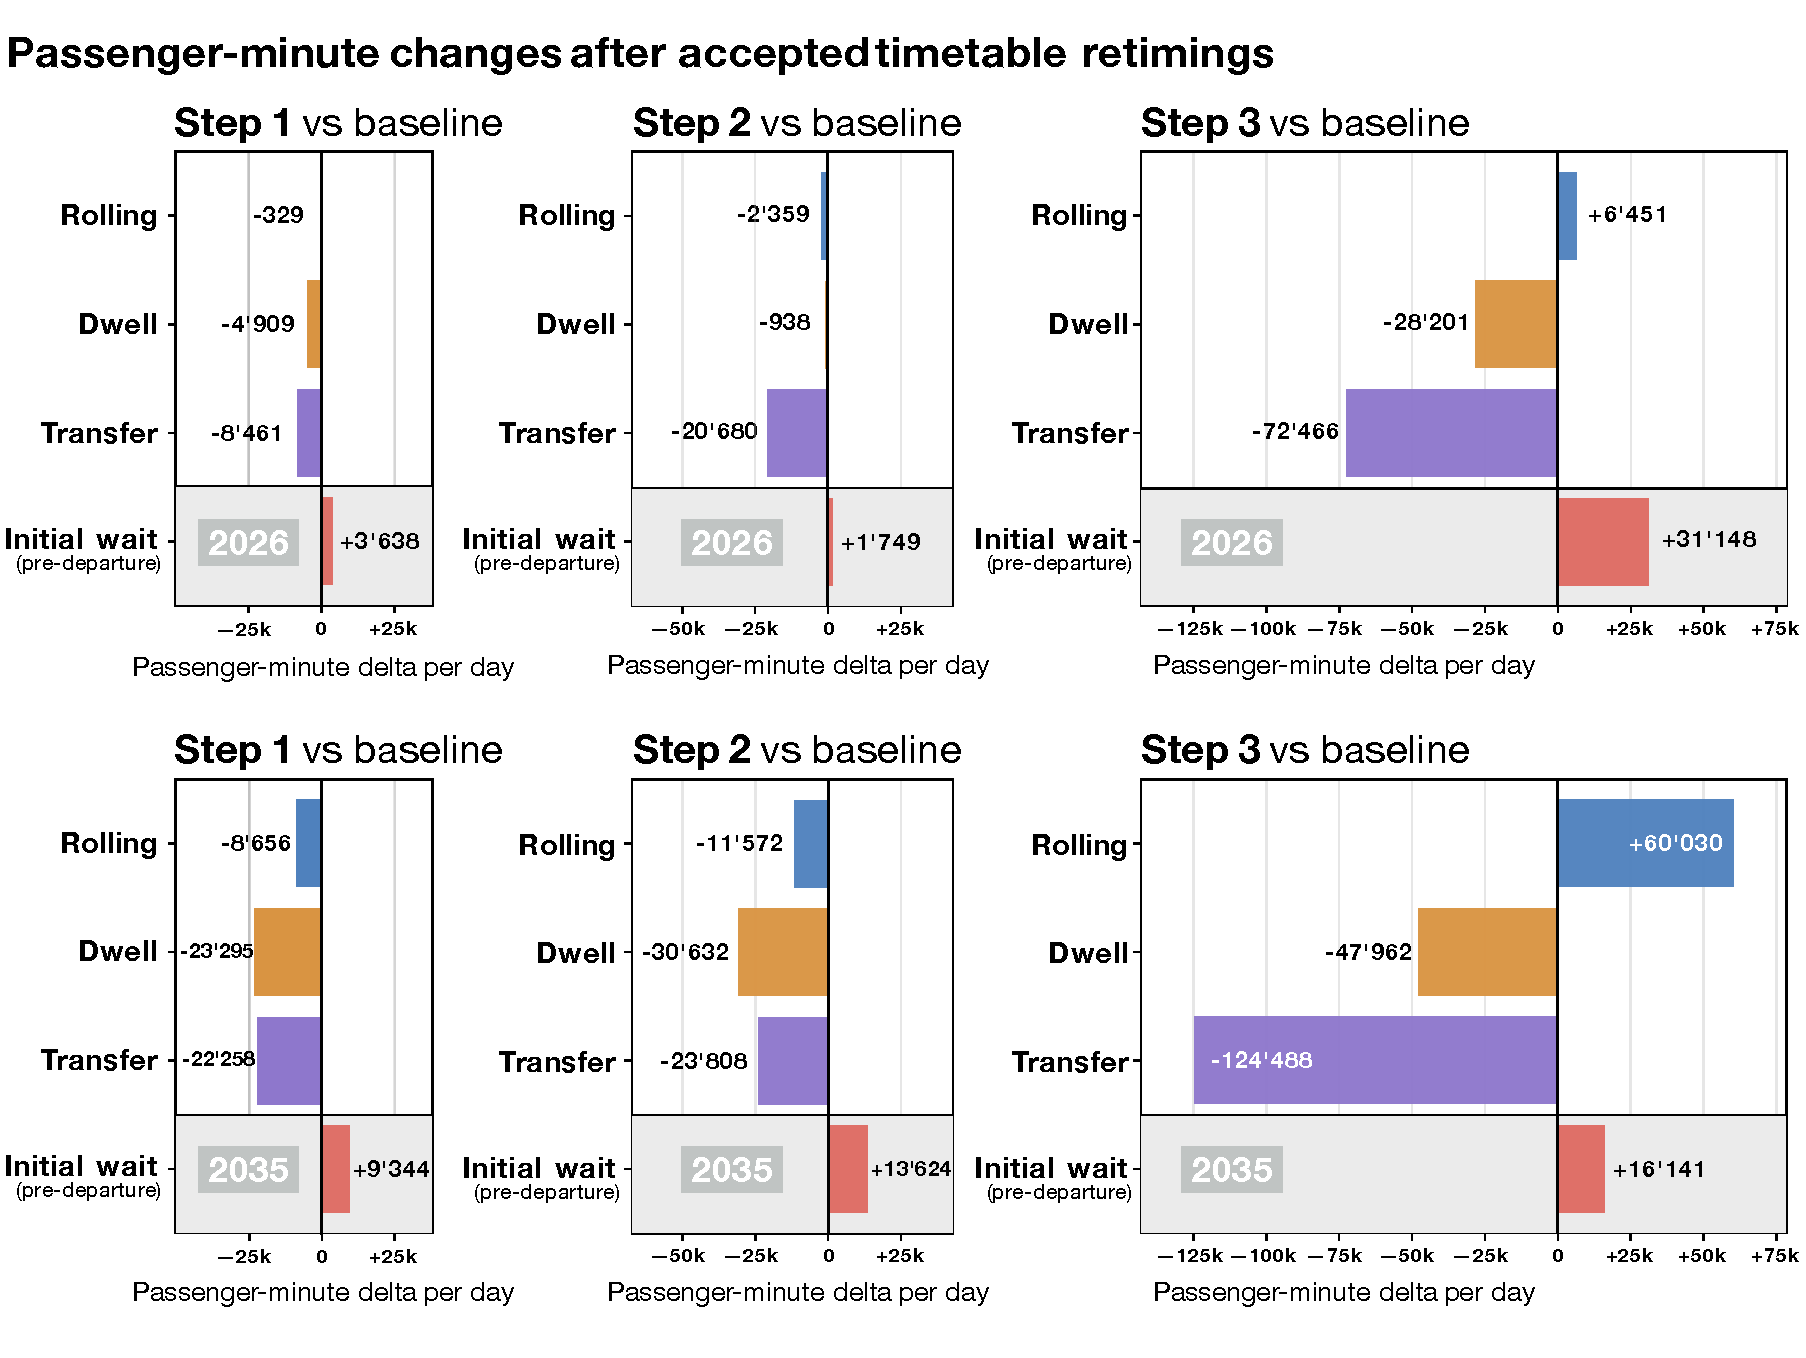
\includegraphics[width=\textwidth]{figures/part-II/part2_national_component_deltas.pdf}
\caption[Passenger-minute changes by optimization step]{Each optimization step's passenger-minute changes by component. Negative values indicate an improvement over the baseline.}
\label{fig:part2-national-components}
\end{figure}

The component changes in Figure~\ref{fig:part2-national-components} show how the final passenger-minute savings are distributed. In 2026, the Step~3 improvement is driven mainly by transfer and dwell savings: transfer time falls by 72'466 passenger-minutes per day, and dwell time by 28'201, while rolling time increases by 6'451. In 2035, transfer time again provides the largest saving, falling by 124'488 passenger-minutes per day; dwell time falls by 47'962, while rolling time increases by 60'030. The countervailing rolling-time increase is due to slightly longer movement paths being made worthwhile when they reduce end-to-end travel time, as exemplified by the Bern--Neuchâtel segment in Figure~\ref{fig:part2-od_spacetime_graph}. Finally, pre-departure initial waiting time rises by 31'148 passenger-minutes per day in 2026 and 16'141 in 2035; this is due to the cumulative effect of the timetable edits shifting a number of existing 30/60-minute intervals off balance. Initial waiting, defined as half the dominance-weighted average interval between trains, affects the time experienced by a passenger arriving randomly at the origin but is excluded from the reported post-departure total-time objective.


The passenger-weighted national component shares vary only slightly because the accepted retimings alter the routed outcome for a small minority of OD pairs with non-zero demand: 79'554 of 2'114'896 pairs in 2026 (3.76\%) and 71'229 of 2'108'251 in 2035 (3.38\%). Since the reported shares are ratios of cumulative national component passenger-minutes, the unchanged OD pairs dominate the denominator and keep the aggregate percentages stable. In 2026, the national rolling share rises from 84.895\% in the baseline to 85.044\% in Step~3, while the dwell share falls from 7.175\% to 7.135\% and the transfer share from 7.931\% to 7.821\%. In 2035, the rolling share rises from 83.576\% to 83.842\%, the dwell share falls from 7.936\% to 7.869\%, and the transfer share from 8.487\% to 8.289\%. These directional trends coincide with what is to be expected following a system-wide travel-time optimization: a slightly larger share of post-departure passenger time is spent moving toward destinations, while a slightly smaller share is spent in transfers or same-train intermediate stops. Figure~\ref{fig:part2-canton-composition-triangle} shows the cantonal variance of these component shares.

The OD-level P05/P50/P95 columns in Table~\ref{tab:part2-national-summary} show that the optimization does not broadly compress the full travel-time distribution. For total post-departure time, the weighted median remains unchanged in both years, and the upper tail also moves only slightly. This means that for most positive-demand OD pairs, the typical routed total time is unchanged even after the accepted retimings. The national savings therefore come from improvements on a small subset of passenger-relevant OD pairs. The reported percentiles describe the distribution of OD-level travel times across OD pairs with non-zero demand, using daily OD demand as the percentile weight.

\begin{table}[htbp]
\centering
\caption[Distribution of post-optimization OD-cell changes]{Distribution of OD-cell changes after Optimized Step~3 relative to baseline. Mean changes are passenger-weighted; percentiles are weighted empirical quantiles across positive-demand OD cells. Negative values indicate lower time in Step~3.}
\label{tab:part2-distributional-step3}
\resizebox{\textwidth}{!}{%
\begin{tabular}{llrrrrrrrrr}
\toprule
\textbf{Year} & \textbf{Metric} & \textbf{Mean change} & \textbf{$\Delta$ pax-min/day} & \textbf{P01} & \textbf{P50} & \textbf{P99} & \textbf{Min} & \textbf{Max} & \textbf{Changed OD} & \textbf{Changed OD} \\
 & & \textbf{[s/trip]} & & \textbf{[min]} & \textbf{[min]} & \textbf{[min]} & \textbf{[min]} & \textbf{[min]} & \textbf{[count]} & \textbf{[\%]} \\
\midrule
2026 & Total & -2.78 & -94'216 & -1.059 & 0.000 & 0.170 & -40.5 & 60.0 & 79'554 & 3.76 \\
2026 & Rolling & 0.19 & 6'451 & -0.275 & 0.000 & 0.340 & -48.1 & 34.7 & 79'554 & 3.76 \\
2026 & Dwell & -0.83 & -28'201 & -0.822 & 0.000 & 0.496 & -18.0 & 22.5 & 79'554 & 3.76 \\
2026 & Transfer & -2.14 & -72'466 & -1.053 & 0.000 & 0.303 & -51.0 & 60.0 & 79'554 & 3.76 \\
2026 & Initial wait & 0.92 & 31'148 & -0.103 & 0.000 & 0.304 & -29.7 & 15.9 & 79'554 & 3.76 \\
\midrule
2035 & Total & -3.12 & -112'419 & -1.178 & 0.000 & 0.133 & -150.0 & 38.0 & 71'229 & 3.38 \\
2035 & Rolling & 1.67 & 60'030 & -0.345 & 0.000 & 0.099 & -125.5 & 150.0 & 71'229 & 3.38 \\
2035 & Dwell & -1.33 & -47'962 & -0.910 & 0.000 & 0.234 & -26.3 & 17.2 & 71'229 & 3.38 \\
2035 & Transfer & -3.46 & -124'488 & -0.469 & 0.000 & 0.504 & -157.7 & 48.0 & 71'229 & 3.38 \\
2035 & Initial wait & 0.45 & 16'141 & -0.115 & 0.000 & 0.326 & -29.1 & 35.8 & 71'229 & 3.38 \\
\bottomrule
\end{tabular}%
}
\end{table}

Table~\ref{tab:part2-distributional-step3} extends the scenario-level values in Table~\ref{tab:part2-national-summary} by reporting OD-level changes after the final Step~3 optimization relative to the baseline. Each OD-cell value is first formed from the available path alternatives using the dominance-minute path shares in Equation~\eqref{eq:part2-path-share} and the corresponding allocated path flows in Equation~\eqref{eq:part2-path-demand}, yielding OD-level mean quantities of the form shown in Equation~\eqref{eq:part2-od-mean-cost}. The OD-cell change distribution is then summarized across positive-demand OD cells. Here, the weighted median change is zero for every metric in both years. The national gain is therefore not produced by a broad shift of the full OD matrix, but by a smaller subset of altered OD pairs: 79'554 non-zero-demand OD cells in 2026 (3.76\%) and 71'229 in 2035 (3.38\%). The 1st percentile total-time improvement reaches -1.059 minutes in 2026 and -1.178 minutes in 2035, while the 99th percentile remains below a 0.2-minute worsening in both years. The extreme minimum and maximum values occur where a local retiming changes the retained dominant path or the retained transfer structure of a transfer-sensitive OD pair, producing a large OD-specific effect without materially changing the shape of the national distribution.

Figure~\ref{fig:part2-histogram} shows the same concentration from the origin side. For each origin station, the figure plots the passenger-weighted mean total-time change of trips starting there, again relative to the baseline. The logarithmic y-axis makes clear that most station origins lie very close to zero, while only a comparatively small number of origins experience sizeable average gains or losses. Figure~\ref{fig:part2-histogram2} makes this pattern even clearer with full OD-pair counts linked with their respective changes in total time, where the OD weighting follows the allocated daily path flows from Equations~\eqref{eq:part2-path-share} and \eqref{eq:part2-path-demand}. In both years, the mass of OD pairs is concentrated near zero change, with the near-zero region dominating by several orders of magnitude. However, many OD pairs see time improvements of several minutes, up to 1 hour. In short, the optimization is very selective in spatial and OD coverage, but where it does act, it can produce substantial improvements for the affected transfer-dependent OD pairs.

\begin{figure}[htb]
\centering
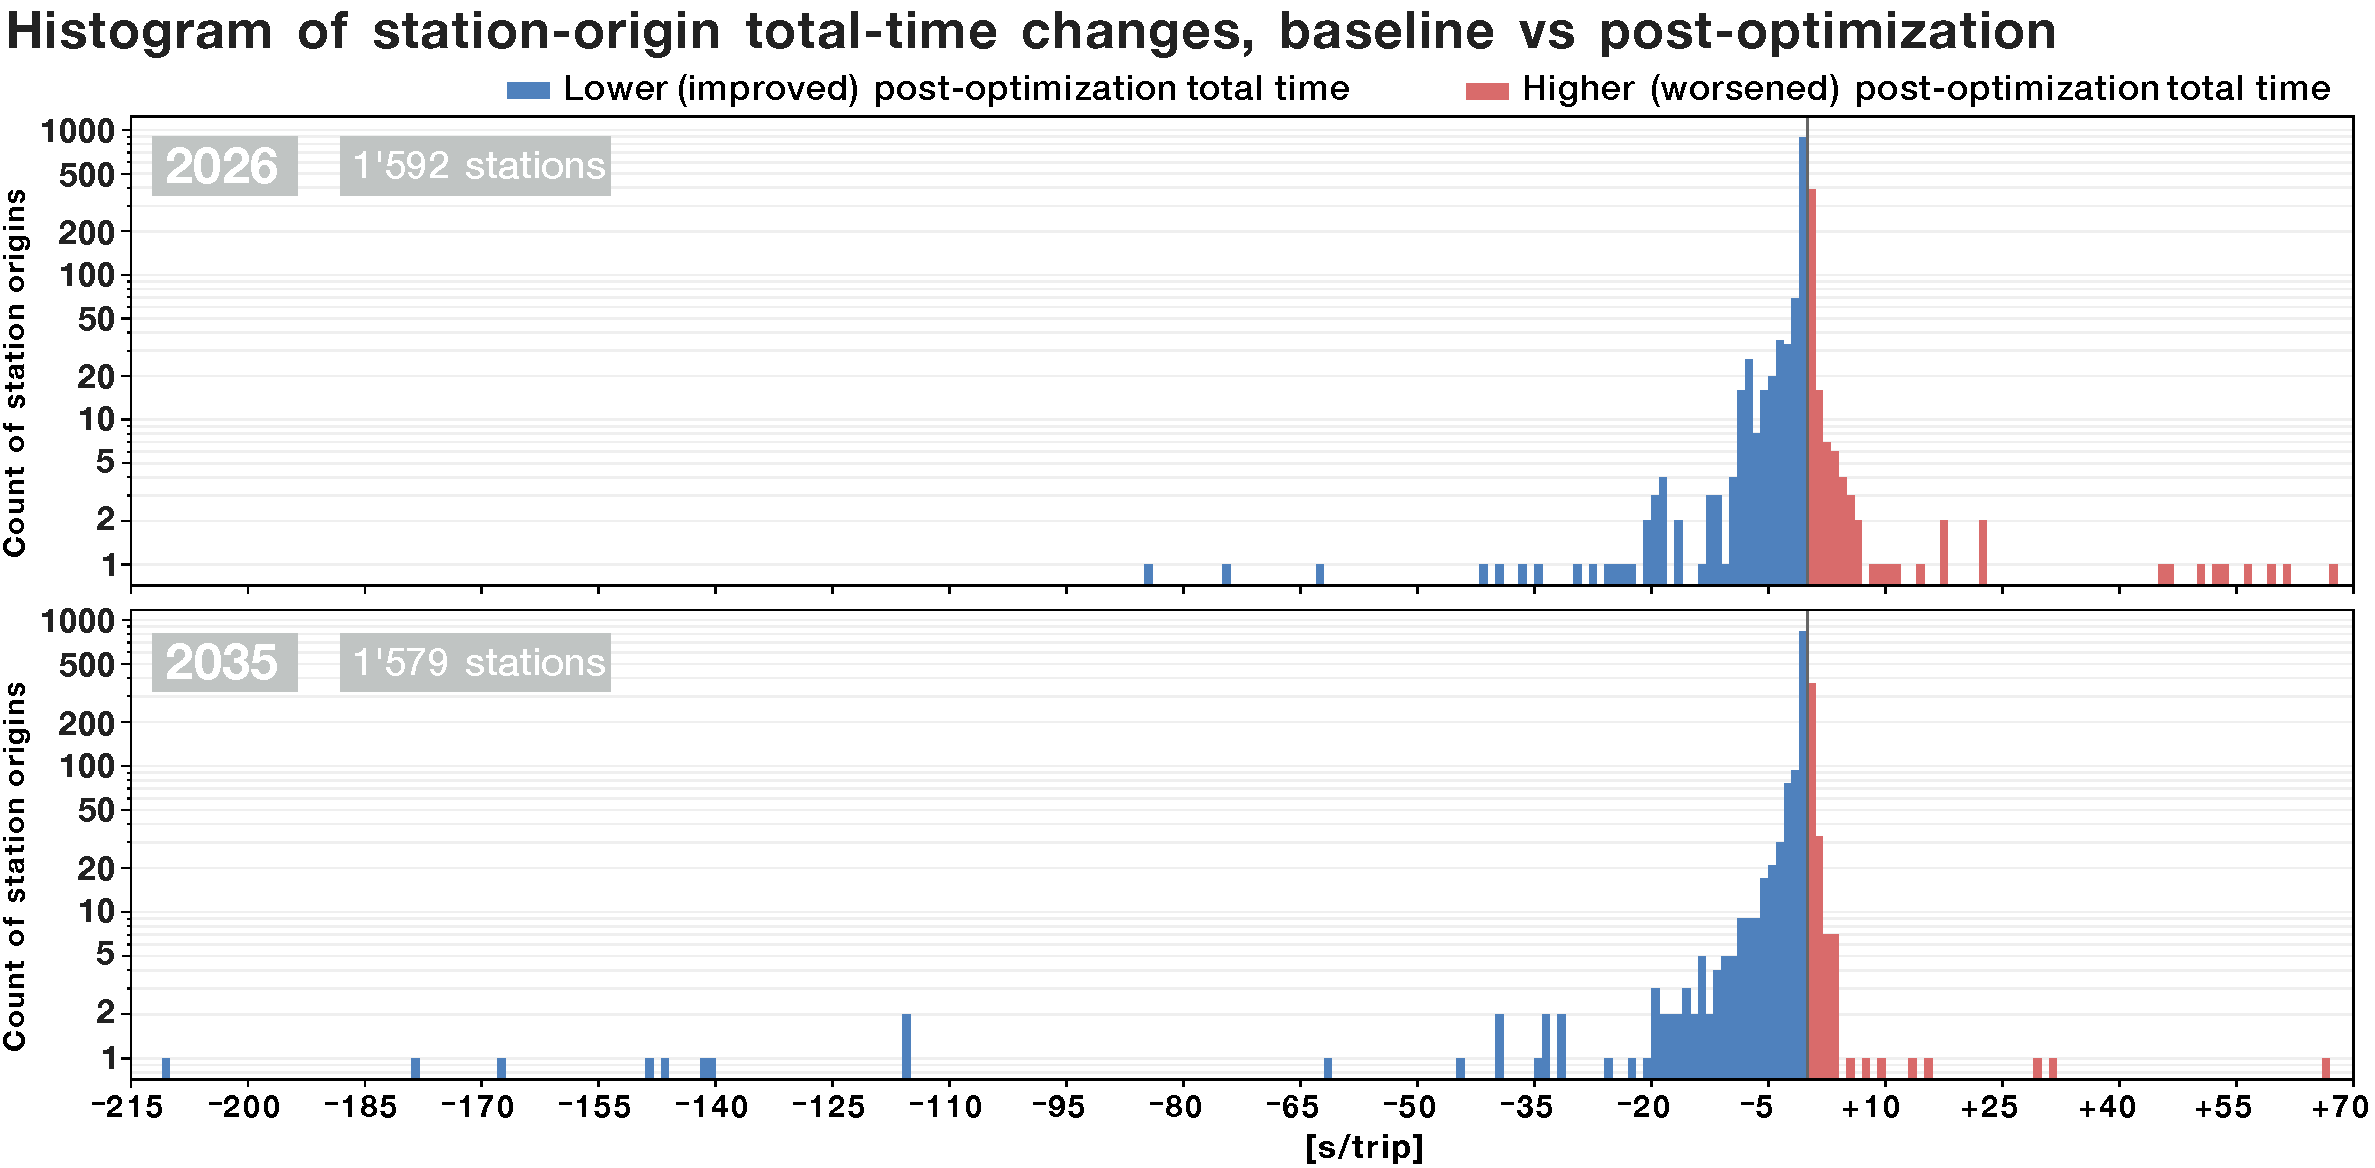
\includegraphics[width=\textwidth]{figures/part-II/part2_station_total_time_histogram_step3_logbins.pdf}
\caption[Histogram of station-origin changes]{Logarithmic histogram counting station origins by their passenger-weighted average total-time change after Optimized Step~3, relative to the baseline, using 1-second bins.}

\label{fig:part2-histogram}
\end{figure}

\begin{figure}[htb]
\centering
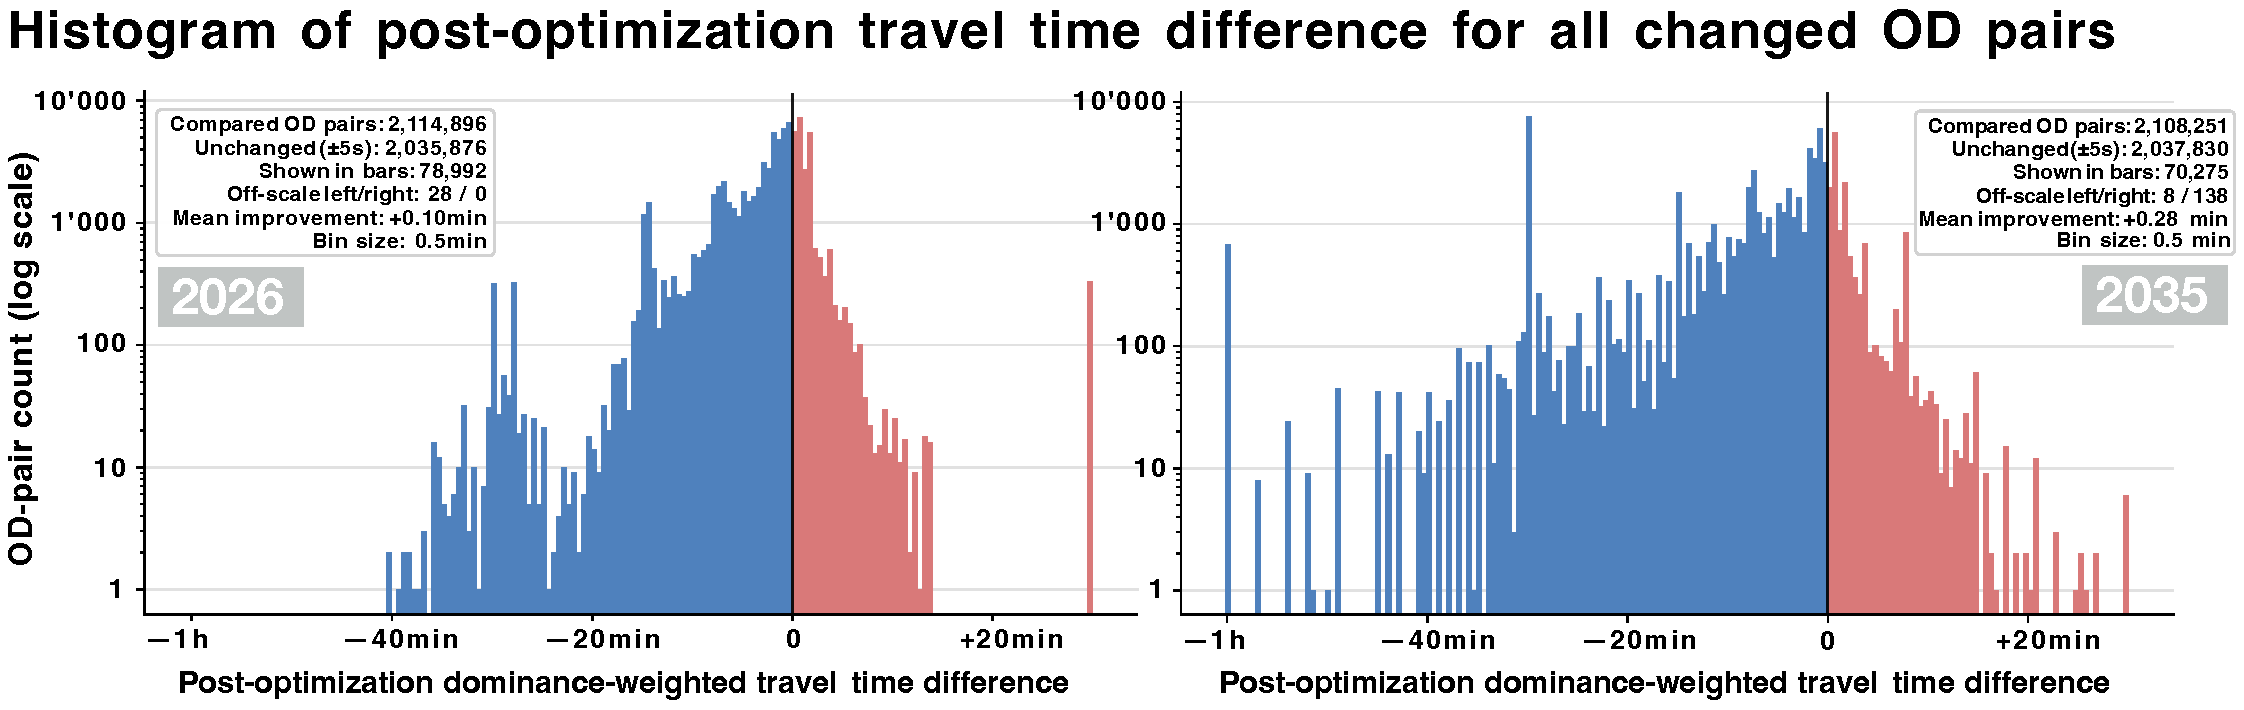
\includegraphics[width=\textwidth]{figures/part-II/part2_step3_od_pair_time_change_histograms.pdf}
\caption[Histogram of OD-pair changes]{Logarithmic histograms of OD-pair count total-time changes post-optimization relative to baseline, using 30-second bins. Blue values indicate faster Step~3 travel times. OD pairs within $\pm 5$ seconds are omitted from the bars and counted as unchanged.}
\label{fig:part2-histogram2}
\end{figure}


\subsection{Accepted timetable edits and transfer mechanisms}\label{sec:results-part2-mechanisms}


\begin{table}[H]
\centering
\caption[National passenger-minute savings by scenario]{National scenario savings; positive savings indicate fewer post-departure passenger-minutes/day.}
\label{tab:part2-selection-summary}
\resizebox{0.85\textwidth}{!}{%
\begin{tabular}{llrrrrr}
\toprule
\textbf{Year} & \textbf{Scenario} & \textbf{Edits} & \textbf{Edits} & \textbf{Active edits} & \textbf{Scenario saving} & \textbf{Additional saving} \\
 & & added& reversed& total&\textbf{[pax-min/day]}&vs prior scenario \\
\midrule
2026 & Optimized Step~1 & 7 & 0 & 7 & 13'699 & 13'699 \\
2026 & Optimized Step~2 & 9 & 0 & 16 & 23'977 & 10'278 \\
2026 & Optimized Step~3 & 26 & 0 & 42 & 94'216 & 70'239 \\
\midrule
2035 & Optimized Step~1 & 11 & 0 & 11 & 54'210 & 54'210 \\
2035 & Optimized Step~2 & 10 & 0 & 21 & 66'012 & 11'803 \\
2035 & Optimized Step~3 & 18 & 2 & 37 & 112'419 & 46'407 \\
\bottomrule
\end{tabular}%
}
\end{table}

Table~\ref{tab:part2-selection-summary} connects the intermediate construction stages with the final scenario-level totals. The added edits should be read cumulatively: Step~2 starts from the validated Step~1 timetable, and Step~3 starts from the validated Step~2 timetable. The two Step~3 edit reversals in 2035 undo earlier potential retiming candidates identified in the prior steps after the combined Step~3 attribution review evaluated their effect on the network negatively through a full OD rebuild. 


Figure~\ref{fig:part2-accepted-edits} maps all accepted timetabled line edits in 2026 and 2035. The optimization candidates are geographically spread out across the country, with 2026 seeing most of the far-flung candidates accepted in Step~3 after the previous steps found only candidates in the northeast. 2035's accepted edits lie principally in major clusters around Bern and Zurich, with minor linked pairs scattered elsewhere.




\begin{figure}[htb]
\centering
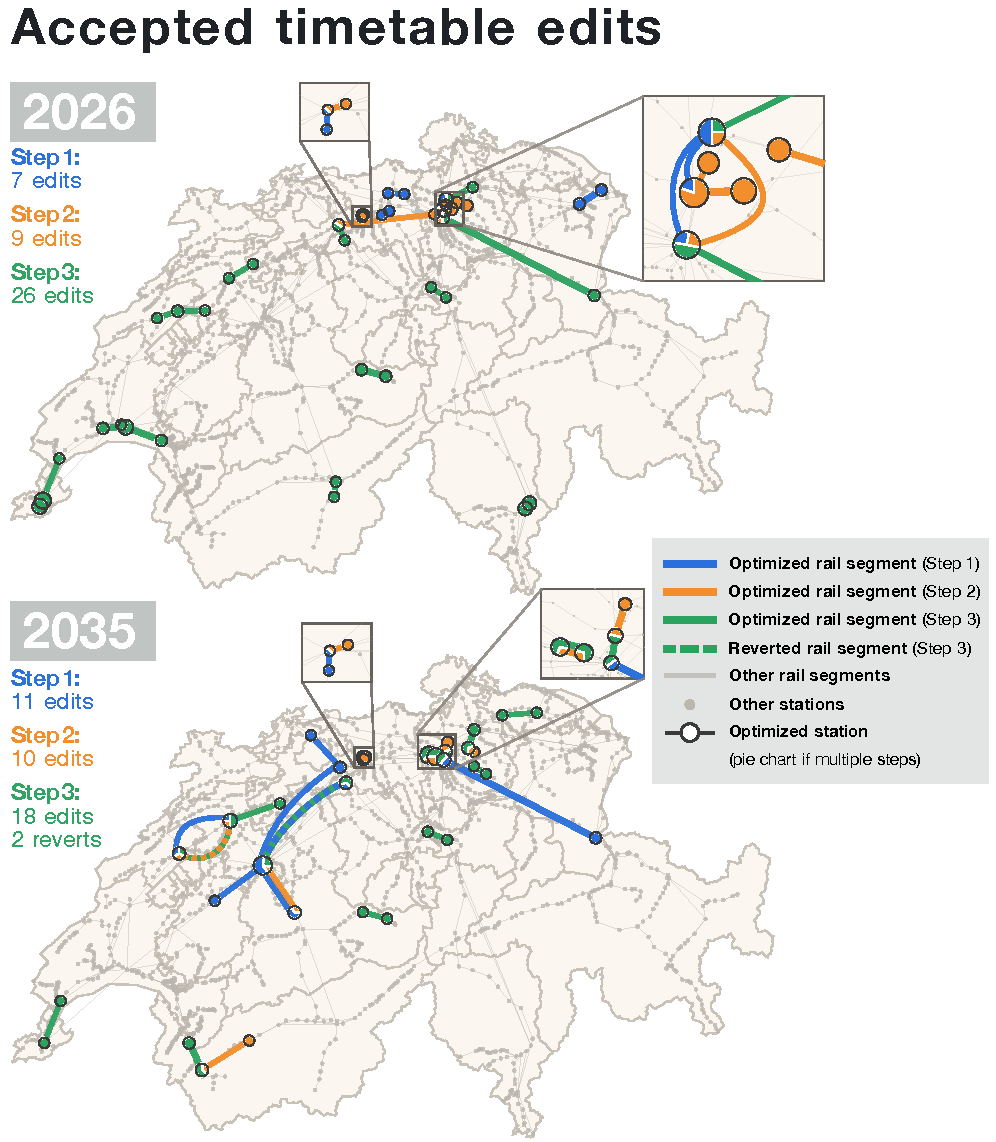
\includegraphics[width=0.85\textwidth]{figures/part-II/part2_accepted_timetable_edits.pdf}
\caption[Map of accepted timetable edits]{Map of accepted timetable edits, colour-coded to differentiate edits accepted in each step.}

\label{fig:part2-accepted-edits}
\end{figure}

Tables~\ref{tab:part2-accepted-edits-2026} and~\ref{tab:part2-accepted-edits-2035} list these accepted timetabled line edits in 2026 and 2035, respectively. Each row in the tables shows one edited line segment in the two-hour clockface representation used by the timetable parser, mapped onto a departure window starting at 05:00. For the diagnostic line-edit attribution columns, ``Affected OD pairs'' counts non-zero-demand OD pairs associated with the listed edit, while the improved and worsened columns report the affected relations with a non-zero attributed change in each direction. ``Affected demand'' is the daily passenger flow associated with each edited segment in the ex-post attribution, and ``Attributed saving'' is the corresponding passenger-minute change. Summing these values cannot precisely reproduce the national result reported in Chapter~\ref{sec:results-part2-national}, because the same OD pair can be associated with more than one accepted edit and the scenarios are evaluated only after all retained edits are applied together. Despite the \(\pm10\)-minute candidate-shift domain defined in Equation~\eqref{eq:part2-shift-domain}, nearly all accepted edits retime the affected section by only one or two minutes, as shown in the \(\boldsymbol{\delta}\) columns.


\begin{table}[!htb]
\centering
\scriptsize
\setlength{\tabcolsep}{2.3pt}
\caption[Accepted 2026 timetable edits]{Accepted 2026 timetable edits and edit-level attributed savings. Bold times denote retimed values. Positive attributed savings indicate fewer passenger-minutes per day for the affected OD pairs.}

\label{tab:part2-accepted-edits-2026}
\resizebox{\textwidth}{!}{%
\begin{tabular}{lllcccccrrrrrr}
\toprule
\textbf{Step} & \textbf{Line} & \textbf{Segment origin}  & \shortstack{\textbf{Old}\\\textbf{start}} & \shortstack{\textbf{New}\\\textbf{start}} & \shortstack{\textbf{New}\\\textbf{end}} & \shortstack{\textbf{Old}\\\textbf{end}} & \shortstack{\textbf{Segment}\\\textbf{destination}}  & \(\boldsymbol{\delta}\) & \shortstack{\textbf{Affected}\\\textbf{OD pairs}} & \shortstack{\textbf{Improved}\\\textbf{OD pairs}} & \shortstack{\textbf{Worsened}\\\textbf{OD pairs}} & \shortstack{\textbf{Affected}\\\textbf{demand}\\\textbf{[pax/day]}} & \shortstack{\textbf{Attributed}\\\textbf{saving}\\\textbf{[pax-min}\\\textbf{/day]}} \\
\midrule
Step~1 & IC~1 & Zürich Oerlikon & 05:44 & \textbf{05:46} & \textbf{05:51} & 05:49 & Zürich Flughafen & \(+2\) & 10'024 & 9'535 & 489 & 34'567 & 2'637 \\
Step~1 & IR~13 & Rorschach & 05:51 & \textbf{05:50} & \textbf{07:03} & 07:04 & St. Gallen & \(-1\) & 176 & 133 & 43 & 3'362 & 679 \\
Step~1 & IR~13 & St. Gallen & 05:55 & \textbf{05:56} & \textbf{06:09} & 06:08 & Rorschach & \(+1\) & 880 & 751 & 129 & 3'705 & 1'526 \\
Step~1 & S~14 & Aarau & 05:24 & \textbf{05:25} & \textbf{05:26} & 05:25 & Binzenhof & \(+1\) & 789 & 59 & 730 & 1'098 & 1'319 \\
Step~1 & IR~75 & Zürich HB & 05:34 & \textbf{05:35} & \textbf{05:45} & 05:44 & Zürich Flughafen & \(+1\) & 17'103 & 14'218 & 2'885 & 25'629 & 2'993 \\
Step~1 & S~23 & Lenzburg & 05:29 & \textbf{05:31} & \textbf{05:34} & 05:32 & Othmarsingen & \(+2\) & 415 & 170 & 245 & 5'537 & 2'199 \\
Step~1 & IR~36 & Brugg AG & 05:00 & \textbf{05:01} & \textbf{05:08} & 05:07 & Baden & \(+1\) & 1'331 & 1'284 & 47 & 9'197 & 4'905 \\
\midrule
Step~2 & IR~75 & Zürich Flughafen & 05:15 & \textbf{05:14} & \textbf{05:25} & 05:26 & Zürich HB & \(-1\) & 19'979 & 15'848 & 4'131 & 32'137 & 3'336 \\
Step~2 & S~14 & Zürich Oerlikon & 05:48 & \textbf{05:47} & \textbf{05:50} & 05:51 & Wallisellen & \(-1\) & 1'248 & 1'222 & 26 & 21'121 & 2'356 \\
Step~2 & S~14 & Zürich Oerlikon & 05:18 & \textbf{05:17} & \textbf{05:20} & 05:21 & Wallisellen & \(-1\) & 1'097 & 1'069 & 28 & 20'693 & 2'306 \\
Step~2 & IR~35 & Zürich Altstetten & 05:59 & \textbf{05:58} & \textbf{06:27} & 06:28 & Olten & \(-1\) & 1'081 & 678 & 403 & 9'185 & 917 \\
Step~2 & S~14 & Aarau & 05:56 & \textbf{05:53} & \textbf{05:54} & 05:57 & Aarau Torfeld & \(-3\) & 853 & 832 & 21 & 4'819 & 1'350 \\
Step~2 & S~7 & Bassersdorf & 05:08 & \textbf{05:11} & \textbf{05:17} & 05:14 & Effretikon & \(+3\) & 251 & 234 & 17 & 5'189 & 704 \\
Step~2 & S~7 & Bassersdorf & 05:38 & \textbf{05:41} & \textbf{05:47} & 05:44 & Effretikon & \(+3\) & 319 & 262 & 57 & 5'395 & 728 \\
Step~2 & S~14 & Wallisellen & 05:09 & \textbf{05:10} & \textbf{05:13} & 05:12 & Zürich Oerlikon & \(+1\) & 1'237 & 1'159 & 78 & 19'949 & 805 \\
Step~2 & S~9 & Zürich Oerlikon & 05:45 & \textbf{05:44} & \textbf{05:46} & 05:47 & Glattbrugg & \(-1\) & 1'183 & 1'158 & 25 & 15'258 & 846 \\
\midrule
Step~3 & IR~15 & Morges & 05:26 & \textbf{05:24} & \textbf{05:35} & 05:37 & Lausanne & \(-2\) & 130'046 & 4'689 & 2'214 & 42'259 & 6'662 \\
Step~3 & IR~15 & Genève & 05:54 & \textbf{05:56} & \textbf{06:09} & 06:07 & Nyon & \(+2\) & 41'670 & 1'208 & 316 & 17'928 & 6'441 \\
Step~3 & S~10 & Giubiasco & 05:39 & \textbf{05:37} & \textbf{05:41} & 05:43 & Bellinzona & \(-2\) & 11'074 & 79 & 701 & 15'603 & 22'152 \\
Step~3 & IR~66 & Ins & 05:18 & \textbf{05:16} & \textbf{05:26} & 05:28 & Neuchâtel & \(-2\) & 45'285 & 1'366 & 1'507 & 9'704 & 2'494 \\
Step~3 & S~10 & Giubiasco & 05:09 & \textbf{05:07} & \textbf{05:11} & 05:13 & Bellinzona & \(-2\) & 11'369 & 75 & 1'210 & 15'523 & 22'100 \\
Step~3 & L~4 & Genève & 05:16 & \textbf{05:17} & \textbf{05:22} & 05:21 & Lancy-Pont-Rouge & \(+1\) & 6'735 & 159 & 271 & 27'200 & 6'422 \\
Step~3 & L~4 & Lancy-Pont-Rouge & 05:52 & \textbf{05:51} & \textbf{05:57} & 05:58 & Genève & \(-1\) & 6'842 & 270 & 1'111 & 24'594 & 2'718 \\
Step~3 & L~2 & Genève & 05:46 & \textbf{05:47} & \textbf{05:52} & 05:51 & Lancy-Pont-Rouge & \(+1\) & 6'992 & 158 & 206 & 27'320 & 6'387 \\
Step~3 & RE~33 & Genève & 05:23 & \textbf{05:25} & \textbf{05:30} & 05:28 & Lancy-Pont-Rouge & \(+2\) & 52'920 & 960 & 633 & 77'255 & 9'134 \\
Step~3 & IR~70 & Zürich Flughafen & 05:23 & \textbf{05:21} & \textbf{05:34} & 05:36 & Winterthur & \(-2\) & 38'256 & 1'301 & 535 & 60'297 & 4'494 \\
Step~3 & IC~51 & Grenchen Nord & 05:31 & \textbf{05:29} & \textbf{05:39} & 05:41 & Biel/Bienne & \(-2\) & 59'973 & 3'660 & 1'693 & 22'377 & 4'649 \\
Step~3 & R~42 & Stalden-Saas & 05:08 & \textbf{05:06} & \textbf{05:17} & 05:19 & Visp & \(-2\) & 2'828 & 16 & 257 & 7'120 & 1'298 \\
Step~3 & R~1 & Lausanne & 05:38 & \textbf{05:39} & \textbf{05:42} & 05:41 & Prilly-Malley & \(+1\) & 18'209 & 457 & 450 & 31'667 & 1'100 \\
Step~3 & IR~95 & Lausanne & 05:52 & \textbf{05:53} & \textbf{06:04} & 06:03 & Morges & \(+1\) & 54'944 & 1'712 & 1'638 & 54'509 & 3'044 \\
Step~3 & S~3 & Immensee & 05:30 & \textbf{05:29} & \textbf{05:37} & 05:38 & Arth-Goldau & \(-1\) & 12'368 & 949 & 743 & 6'588 & 1'144 \\
Step~3 & S~10 & Bellinzona & 05:46 & \textbf{05:48} & \textbf{05:52} & 05:50 & Giubiasco & \(+2\) & 12'032 & 81 & 1'213 & 18'460 & 6'436 \\
Step~3 & IC~3 & Zürich HB & 05:07 & \textbf{05:08} & \textbf{06:03} & 06:02 & Sargans & \(+1\) & 53'505 & 2'242 & 1'304 & 16'946 & 4'677 \\
Step~3 & IC~3 & Zürich HB & 05:38 & \textbf{05:39} & \textbf{06:33} & 06:32 & Sargans & \(+1\) & 83'455 & 2'969 & 2'020 & 15'464 & 4'808 \\
Step~3 & L~4 & Lancy-Pont-Rouge & 05:37 & \textbf{05:36} & \textbf{05:42} & 05:43 & Genève & \(-1\) & 8'462 & 289 & 294 & 27'237 & 2'733 \\
Step~3 & IR~95 & Vevey & 05:30 & \textbf{05:29} & \textbf{05:45} & 05:46 & Lausanne & \(-1\) & 54'944 & 1'712 & 1'638 & 54'509 & 3'044 \\
Step~3 & S~10 & Bellinzona & 05:16 & \textbf{05:18} & \textbf{05:22} & 05:20 & Giubiasco & \(+2\) & 10'731 & 92 & 656 & 16'071 & 6'493 \\
Step~3 & IR~66 & Chambrelien & 05:21 & \textbf{05:19} & \textbf{05:28} & 05:30 & Neuchâtel & \(-2\) & 49'676 & 1'407 & 1'940 & 9'844 & 1'494 \\
Step~3 & PE & Meiringen & 05:22 & \textbf{05:26} & \textbf{05:37} & 05:33 & Brienz & \(+4\) & 20'660 & 1'031 & 722 & 5'620 & 1'629 \\
Step~3 & PE & Brienz & 05:25 & \textbf{05:21} & \textbf{05:31} & 05:35 & Meiringen & \(-4\) & 18'448 & 1'071 & 530 & 5'270 & 1'282 \\
Step~3 & IR~95 & Lausanne & 05:14 & \textbf{05:15} & \textbf{05:29} & 05:28 & Vevey & \(+1\) & 53'172 & 1'282 & 1'231 & 41'784 & 7'327 \\
Step~3 & IR~27 & Zofingen & 05:03 & \textbf{05:01} & \textbf{05:08} & 05:10 & Olten & \(-2\) & 15'035 & 202 & 376 & 30'595 & 1'239 \\
\bottomrule
\end{tabular}%
}
\end{table}

\begin{table}[!htb]
\centering
\scriptsize
\setlength{\tabcolsep}{2.3pt}
\caption[Accepted 2035 timetable edits]{Accepted 2035 timetable edits and edit-level attributed savings. Bold times denote retimed values. Positive attributed savings indicate fewer passenger-minutes per day for the affected OD pairs.}
\label{tab:part2-accepted-edits-2035}
\resizebox{\textwidth}{!}{%
\begin{tabular}{lllcccccrrrrrr}
\toprule
\textbf{Step} & \textbf{Line} & \textbf{Segment origin}  & \shortstack{\textbf{Old}\\\textbf{start}} & \shortstack{\textbf{New}\\\textbf{start}} & \shortstack{\textbf{New}\\\textbf{end}} & \shortstack{\textbf{Old}\\\textbf{end}} & \shortstack{\textbf{Segment}\\\textbf{destination}}  & \(\boldsymbol{\delta}\) & \shortstack{\textbf{Affected}\\\textbf{OD pairs}} & \shortstack{\textbf{Improved}\\\textbf{OD pairs}} & \shortstack{\textbf{Worsened}\\\textbf{OD pairs}} & \shortstack{\textbf{Affected}\\\textbf{demand}\\\textbf{[pax/day]}} & \shortstack{\textbf{Attributed}\\\textbf{saving}\\\textbf{[pax-min}\\\textbf{/day]}} \\
\midrule
Step~1 & IC~61 & Olten & 05:31 & \textbf{05:27} & \textbf{05:54} & 05:58 & Bern & \(-4\) & 4'934 & 2'867 & 2'067 & 10'137 & 4'168 \\
Step~1 & IC~1 & Fribourg/Freiburg & 05:36 & \textbf{05:34} & \textbf{05:54} & 05:56 & Bern & \(-2\) & 17'737 & 15'680 & 2'057 & 12'702 & 5'179 \\
Step~1 & IC~61 & Thun & 05:37 & \textbf{05:35} & \textbf{05:54} & 05:56 & Bern & \(-2\) & 3'219 & 2'105 & 1'114 & 12'798 & 2'353 \\
Step~1 & IC~61 & Bern & 05:04 & \textbf{05:06} & \textbf{05:24} & 05:22 & Thun & \(+2\) & 2'371 & 1'314 & 1'057 & 12'344 & 200 \\
Step~1 & IC~82 & Zofingen & 05:32 & \textbf{05:31} & \textbf{05:59} & 06:00 & Bern & \(-1\) & 1'977 & 1'163 & 814 & 3'957 & -662 \\
Step~1 & IC~5 & Biel/Bienne & 05:15 & \textbf{05:16} & \textbf{05:34} & 05:33 & Neuchâtel & \(+1\) & 6'181 & 4'670 & 1'511 & 6'420 & 1'638 \\
Step~1 & S~14 & Aarau & 05:24 & \textbf{05:25} & \textbf{05:26} & 05:25 & Binzenhof & \(+1\) & 4'813 & 3'336 & 1'477 & 4'915 & 25'413 \\
Step~1 & S~14 & Aarau & 05:54 & \textbf{05:55} & \textbf{05:56} & 05:55 & Binzenhof & \(+1\) & 4'825 & 3'377 & 1'448 & 4'945 & 25'740 \\
Step~1 & IC~3 & Sargans & 05:28 & \textbf{05:26} & \textbf{06:20} & 06:22 & Zürich HB & \(-2\) & 5'752 & 2'896 & 2'856 & 4'427 & 12'466 \\
Step~1 & IC~3 & Sargans & 05:58 & \textbf{05:56} & \textbf{06:50} & 06:52 & Zürich HB & \(-2\) & 4'361 & 2'050 & 2'311 & 4'374 & 12'506 \\
Step~1 & IC~61 & Liestal & 05:08 & \textbf{05:07} & \textbf{05:24} & 05:25 & Olten & \(-1\) & 2'087 & 1'026 & 1'061 & 9'550 & 4'579 \\
\midrule
Step~2 & IC~82 & Bern & 05:06 & \textbf{05:08} & \textbf{05:26} & 05:24 & Thun & \(+2\) & 210 & 165 & 45 & 8'392 & 3'804 \\
Step~2 & IC~5 & Neuchâtel & 05:27 & \textbf{05:25} & \textbf{05:43} & 05:45 & Biel/Bienne & \(-2\) & 4'225 & 856 & 3'369 & 5'977 & -1'660 \\
Step~2 & IR~55 & Zürich Flughafen & 05:31 & \textbf{05:32} & \textbf{05:36} & 05:35 & Zürich Oerlikon & \(+1\) & 198 & 68 & 130 & 18'830 & 3'103 \\
Step~2 & IC~9 & Sion & 05:04 & \textbf{05:06} & \textbf{05:18} & 05:16 & Martigny & \(+2\) & 1'334 & 360 & 974 & 6'346 & 1'966 \\
Step~2 & G & Schlieren & 05:13 & \textbf{05:14} & \textbf{05:18} & 05:17 & Zürich Altstetten & \(+1\) & 868 & 861 & 7 & 13'106 & 2'749 \\
Step~2 & G & Schlieren & 05:43 & \textbf{05:44} & \textbf{05:48} & 05:47 & Zürich Altstetten & \(+1\) & 845 & 837 & 8 & 13'155 & 2'761 \\
Step~2 & IR~55 & Zürich Flughafen & 05:01 & \textbf{05:02} & \textbf{05:06} & 05:05 & Zürich Oerlikon & \(+1\) & 221 & 68 & 153 & 18'925 & 3'110 \\
Step~2 & S~14 & Aarau Torfeld & 05:45 & \textbf{05:47} & \textbf{05:51} & 05:49 & Aarau & \(+2\) & 1'012 & 835 & 177 & 1'479 & 1'207 \\
Step~2 & S~14 & Aarau Torfeld & 05:15 & \textbf{05:17} & \textbf{05:21} & 05:19 & Aarau & \(+2\) & 971 & 784 & 187 & 1'493 & 1'205 \\
Step~2 & P & Effretikon & 05:40 & \textbf{05:37} & \textbf{05:41} & 05:44 & Illnau & \(-3\) & 846 & 842 & 4 & 4'577 & 648 \\
\midrule
Step~3 & IC~5 & Solothurn & 05:54 & \textbf{05:52} & \textbf{06:07} & 06:09 & Biel/Bienne & \(-2\) & 259'974 & 16'614 & 3'298 & 46'340 & 9'208 \\
Step~3 & IC~1 & Weinfelden & 05:09 & \textbf{05:11} & \textbf{05:21} & 05:19 & Frauenfeld & \(+2\) & 253'352 & 8'416 & 3'649 & 56'247 & 6'148 \\
Step~3 & IC~9 & Genève & 05:10 & \textbf{05:12} & \textbf{05:25} & 05:23 & Nyon & \(+2\) & 104'116 & 7'136 & 1'248 & 53'190 & 3'573 \\
Step~3 & VAE & Arth-Goldau & 05:49 & \textbf{05:51} & \textbf{06:01} & 05:59 & Küssnacht am Rigi & \(+2\) & 53'347 & 1'542 & 575 & 19'595 & 3'438 \\
Step~3 & IC~9 & St-Maurice & 05:04 & \textbf{05:02} & \textbf{05:11} & 05:13 & Martigny & \(-2\) & 91'743 & 8'605 & 1'045 & 62'138 & 3'759 \\
Step~3 & IC~9 & Martigny & 05:45 & \textbf{05:47} & \textbf{05:56} & 05:54 & St-Maurice & \(+2\) & 51'462 & 3'820 & 1'068 & 50'493 & 3'747 \\
Step~3 & D & Winterthur & 05:22 & \textbf{05:24} & \textbf{05:31} & 05:29 & Effretikon & \(+2\) & 14'706 & 628 & 185 & 60'106 & 8'121 \\
Step~3 & PE & Meiringen & 05:22 & \textbf{05:26} & \textbf{05:37} & 05:33 & Brienz & \(+4\) & 21'546 & 2'099 & 489 & 5'448 & 1'870 \\
Step~3 & A & Zürich HB & 05:10 & \textbf{05:11} & \textbf{05:16} & 05:15 & Zürich Oerlikon & \(+1\) & 7'049 & 471 & 57 & 49'811 & 3'120 \\
Step~3 & A & Zürich HB & 05:40 & \textbf{05:41} & \textbf{05:46} & 05:45 & Zürich Oerlikon & \(+1\) & 9'822 & 480 & 75 & 57'391 & 3'132 \\
Step~3 & H & Zürich Altstetten & 05:56 & \textbf{05:55} & \textbf{05:58} & 05:59 & Schlieren & \(-1\) & 10'349 & 795 & 40 & 41'089 & 5'436 \\
Step~3 & H & Zürich Altstetten & 05:26 & \textbf{05:25} & \textbf{05:28} & 05:29 & Schlieren & \(-1\) & 9'771 & 805 & 44 & 41'247 & 5'564 \\
Step~3 & G & Zürich Altstetten & 05:41 & \textbf{05:40} & \textbf{05:43} & 05:44 & Schlieren & \(-1\) & 6'230 & 841 & 34 & 56'248 & 10'620 \\
Step~3 & D & Winterthur & 05:52 & \textbf{05:54} & \textbf{06:01} & 05:59 & Effretikon & \(+2\) & 10'111 & 544 & 148 & 18'620 & 7'963 \\
Step~3 & H & Schlieren & 05:29 & \textbf{05:30} & \textbf{05:34} & 05:33 & Zürich Altstetten & \(+1\) & 9'994 & 436 & 37 & 45'670 & 3'401 \\
Step~3 & Q & Wetzikon ZH & 05:32 & \textbf{05:33} & \textbf{05:38} & 05:37 & Uster & \(+1\) & 26'573 & 1'465 & 111 & 51'525 & 1'837 \\
Step~3 & IC~82 & Bern & 05:00 & \textbf{05:01} & \textbf{05:29} & 05:28 & Zofingen & \(+1\) & 59'108 & 8'873 & 881 & 27'988 & 5'672 \\
Step~3 & G & Zürich Altstetten & 05:11 & \textbf{05:10} & \textbf{05:13} & 05:14 & Schlieren & \(-1\) & 6'010 & 855 & 23 & 55'875 & 10'665 \\
\midrule
\rowcolor{black!8}
Step~3 revert & IC~5 & Neuchâtel & 05:25 & \textbf{05:27} & \textbf{05:45} & 05:43 & Biel/Bienne & \(+2\) & 60'239 & 3'370 & 782 & 6'062 & 1'665 \\
\rowcolor{black!8}
Step~3 revert & IC~82 & Zofingen & 05:31 & \textbf{05:32} & \textbf{06:00} & 05:59 & Bern & \(+1\) & 26'434 & 266 & 214 & 3'873 & 762 \\
\bottomrule
\end{tabular}%
}
\end{table}

% The tables also clarify why row-level attribution must be interpreted carefully. Two earlier 2035 rows, IC~5 Neuchâtel--Biel/Bienne and IC~82 Zofingen--Bern, are shown again as grey Step~3 reversal rows because Step~3 restores those sections to their baseline times. The IC~5 restoration has a positive row-level attribution, whereas the IC~82 restoration has a small negative attribution when considered alone. The restoration set is nevertheless evaluated as part of the complete corrected Step~3 timetable; the national result is determined by the full OD rebuild rather than by requiring every individual attribution row to be positive. The scenario-level result is therefore still the validated change in \(F^{y,\sigma}\), reported in Table~\ref{tab:part2-national-summary}, rather than the sum of the row-level attribution values in Tables~\ref{tab:part2-accepted-edits-2026} and~\ref{tab:part2-accepted-edits-2035}.

Several rows in Tables~\ref{tab:part2-accepted-edits-2026} and~\ref{tab:part2-accepted-edits-2035} are useful anchors for the upcoming spatial interpretation. In 2026, the Step~3 shifts around Bellinzona--Giubiasco and Genève--Lancy-Pont-Rouge correspond to the strong Ticino and Geneva origin effects, while the inherited airport, Oerlikon, and Wallisellen rows remain visible in the Zürich-area pattern. In 2035, the S~14 Aarau--Binzenhof rows and the Step~3 Solothurn--Biel/Bienne shift are consistent with the strong Solothurn/Aargau corridor effects. The grey Neuchâtel--Biel/Bienne reversal also helps explain why Neuchâtel no longer appears among the most worsened cantons. These links are interpretive rather than one-to-one causal allocations: the scenario-level result remains the full objective reported in Table~\ref{tab:part2-national-summary}.
\newpage
The two Step~3 reversal rows in 2035's Table~\ref{tab:part2-accepted-edits-2035} identify the only earlier edits whose local candidate scores were favourable but whose later full-network attribution was negative. Step~1's IC~82 shift satisfied Equation~\eqref{eq:part2-step1-greedy}: its station-board proxy estimated a net saving of \(1'714.83\) passenger-minutes per day, including \(1'832.98\) passenger-minutes of local gain and \(118.15\) passenger-minutes of local loss, while the broken-transfer flow was \(B_z=0\). It therefore passed the positive-proxy and protected-transfer constraints, but the subsequent attribution assigned the edit a saving of \(-662\) passenger-minutes per day. It improved 349 more OD pairs than it worsened, but these pairs were associated with less passenger flow. Similarly, Step~2 IC~5 shift passed the preliminary constraints in Equation~\eqref{eq:part2-step2-static-filter}: its station-board estimates gave \(P^{\mathrm{gain}}_z=923.89\), \(P^{\mathrm{loss}}_z=198.16\), and \(P^{\mathrm{net}}_z=725.73\) passenger-minutes per day, so its loss--gain ratio was \(0.21\), below the \(0.75\) limit. It also produced \(E_z=613.62\) passenger-minutes per day on the fixed Step~1 reference paths, had no invalidated reference-path flow, and a Step~2 score of \(S_z=665.37\), thereby satisfying Equation~\eqref{eq:part2-step2-acceptance-rule}. After the later full OD rebuild, however, its attributed saving was \(-1'660\) passenger-minutes per day, worsening 2'513 more OD pairs than were improved. In both reversal cases, the filtration used gain and loss proxies derived from the surrounding timetable, which provided an effective screening approximation for the other retained edits but did not capture all path-rebuilding and dominance-share responses for these two sections. The Step~3 attribution review exposed these exceptions and restored the affected line segments to their baseline times.

\newpage

The three optimization scenarios differ in their transfer-mechanism composition. Step~1 is more near-miss oriented and therefore identifies many newly unlocked transfers, especially in 2026. The accepted edits in Steps~2 and~3 are dominated by shorter already-feasible transfers because the reference-path evaluation rewards transfer-time reductions on routes already used by passengers. This helps explain why several OD pairs can be negatively affected while their combined passenger-minute loss remains comparatively small. Table~\ref{tab:part2-step3-attribution-summary} reports Step~3's row-level OD associations, affected passenger weights, and attributed passenger-minute change. One OD pair can be associated with several edits.

\begin{table}[htbp]
\centering
\small
\setlength{\tabcolsep}{3.2pt}
\caption[Step~3 row-level attribution summary]{Step~3 row-level attribution summary. Positive attributed savings indicate lower pax-min.}
\label{tab:part2-step3-attribution-summary}
\resizebox{\textwidth}{!}{%
\begin{tabular}{c l r r r r r r r r}
\toprule
\textbf{Year} & \textbf{Row group} & \textbf{Rows} & \textbf{Sum} & \textbf{Median} & \textbf{Max} & \textbf{Improved} & \textbf{Worsened} & \textbf{Affected demand} & \textbf{Attributed saving} \\
 & & & OD pairs & OD pairs &  OD pairs&  OD pairs&  OD pairs& \textbf{[pax/day]} & \textbf{[pax-min/day]} \\
\midrule
2026 & Step~3 additions & 26 & 879'631 & 19'554 & 130'046 & 29'437 & 25'409 & 681'742 & 141'399 \\
2035 & Step~3 additions & 18 & 1'005'263 & 18'126 & 259'974 & 64'425 & 13'007 & 799'022 & 97'275 \\
2035 & Step~3 reversals & 2 & 86'673 & 43'336 & 60'239 & 3'636 & 996 & 9'935 & 903 \\
\bottomrule
\end{tabular}%
}
\end{table}

Figure~\ref{fig:part2-step3-od-path-categories} reframes the Step~3 outcome at the OD-pair level. Each point represents one OD pair with at least 1 passenger per day, and the vertical axis shows the dominance-weighted total post-departure travel-time change relative to the baseline. Negative values indicate faster Step~3 journeys, while positive values indicate slower journeys. 
OD pairs are separated into seven outcome categories. Existing transfers (improved or worsened) keep the same line sequence from origin to destination, but become faster or slower, respectively. Newly unlocked transfers and newly missed transfers mean that the relevant OD pair alters its dominant line sequence. OD pairs with additional non-dominated paths and fewer paths are shown separately to isolate the pairs with altered headways. A large majority of OD pairs are temporally unaffected by the line edits. The lower summary rows report the 5th percentile, median, 95th percentile, and mean travel-time change. The figure shows that the optimized timetable affects only a small subset of passenger-relevant OD pairs, but that the affected pairs are not symmetric in magnitude. In 2026 and 2035, improved existing OD pairs are more numerous than worsened existing pairs and have a lower mean change. Newly missed OD pairs remain comparatively few in both years and have smaller average deteriorations. The path-count categories further show the benefit of a full OD rerouting: timetable edits can lead to a gain or loss of available retained nondominated alternative paths between OD pairs, due to the effects of newly unlocked and missed transfers.

\begin{figure}[H]
\centering

\includegraphics[width=\textwidth]{figures/part-II/part2_step3_od_path_change_category_panels_split_paths_scaled.pdf}
\caption[OD-level Step~3 travel-time changes by path category]{OD-level total travel-time changes after Optimized Step~3 relative to baseline for OD pairs with at least 1 passenger per day. Values are dominance-weighted post-departure total-time changes in minutes per trip. Negative values indicate faster Step~3 journeys and positive values indicate slower journeys. Categories distinguish same dominant line-sequence changes, changed dominant line-sequence changes, changes in the number of retained nondominated paths, and unaffected OD pairs.}
\label{fig:part2-step3-od-path-categories}
\end{figure}





% \begin{table}[htbp]
% \centering
% \small
% \setlength{\tabcolsep}{3.0pt}
% \renewcommand{\arraystretch}{0.82}
% \caption{Transfer mechanisms associated with accepted timetable edits. Mechanism counts are based on the same transfer-line-window grouping for Steps~1--3. Improved-feasible and newly feasible counts refer to unique grouped transfer mechanisms, not to OD pairs. Reported passenger-minute values are the summed local realized transfer gains from that mechanism class.}
% \label{tab:part2-retiming-classes}
% \begin{tabular}{c l r r r r r}
% \toprule
% \textbf{Year} &
% \textbf{Optimization stage} &
% \textbf{Rows} &
% \makecell[r]{\textbf{Improved} \\ \textbf{feasible} \\ \textbf{groups}} &
% \makecell[r]{\textbf{Newly} \\ \textbf{feasible} \\ \textbf{groups}} &
% \makecell[r]{\textbf{Improved} \\ \textbf{feasible gain} \\ \textbf{[pax-min/day]}} &
% \makecell[r]{\textbf{Newly feasible} \\ \textbf{gain} \\ \textbf{[pax-min/day]}} \\
% \midrule
% 2026 & Step~1 additions & 7 & 2 & 8 & 172 & 1'082 \\
% 2026 & Step~2 additions & 9 & 30 & 1 & 7'856 & 76 \\
% 2026 & Step~3 additions & 26 & 6 & 5 & 577 & 380 \\
% \textbf{2026} & \textbf{All accepted edits} & \textbf{42} & \textbf{38} & \textbf{14} & \textbf{8'604} & \textbf{1'538} \\
% \midrule
% 2035 & Step~1 additions & 11 & 9 & 26 & 1'697 & 6'665 \\
% 2035 & Step~2 additions & 10 & 26 & 2 & 4'667 & 401 \\
% 2035 & Step~3 additions & 18 & 19 & 12 & 1'712 & 761 \\
% \textbf{2035} & \textbf{All accepted edits} & \textbf{39} & \textbf{54} & \textbf{40} & \textbf{8'076} & \textbf{7'827} \\
% \bottomrule
% \end{tabular}
% \end{table}

% \begin{table}[htbp]
% \centering
% \small
% \setlength{\tabcolsep}{3.0pt}
% \renewcommand{\arraystretch}{0.82}
% \caption{Transfer mechanisms associated with Step~1 and Step~2 accepted timetable edits. OD-pair counts refer to the number of positive-demand OD pairs associated with accepted edit rows in the mechanism attribution table. Total audited rows combine the retained Step~1 rows and the Step~2 additions for the same year; Step~3 additions are listed in Tables~\ref{tab:part2-accepted-edits-2026} and~\ref{tab:part2-accepted-edits-2035} but are not regrouped in this transfer-mechanism audit.}
% \label{tab:part2-retiming-classes}
% \begin{tabular}{c l r r r r r r}
% \toprule
% \textbf{Year} &
% \textbf{Optimization} &
% \textbf{Rows} &
% \makecell[r]{\textbf{Sum OD}\\\textbf{pairs}} &
% \makecell[r]{\textbf{Median OD}\\\textbf{pairs}} &
% \makecell[r]{\textbf{Max OD}\\\textbf{pairs}} &
% \makecell[r]{\textbf{Improved}\\\textbf{feasible}} &
% \makecell[r]{\textbf{Newly}\\\textbf{feasible}} \\
% \midrule
% 2026 & Step~1 additions & 7 & 101'664 & 5'999 & 51'569 & 2 & 8 \\
% 2026 & Step~2 additions & 9 & 121'659 & 7'921 & 38'068 & 30 & 1 \\
% \textbf{2026} & \textbf{Step~1--2 audited rows} & \textbf{16} & \textbf{223'323} & \textbf{6'556} & \textbf{51'569} & \textbf{32} & \textbf{9} \\
% \midrule
% 2035 & Step~1 additions & 11 & 485'140 & 26'882 & 135'377 & 9 & 26 \\
% 2035 & Step~2 additions & 10 & 171'692 & 7'356 & 57'956 & 26 & 2 \\
% \textbf{2035} & \textbf{Step~1--2 audited rows} & \textbf{21} & \textbf{656'832} & \textbf{22'536} & \textbf{135'377} & \textbf{35} & \textbf{28} \\
% \bottomrule
% \end{tabular}
% \end{table}
\clearpage

\subsection{OD-level passenger examples}\label{sec:results-part2-od-examples}

The OD-level examples in Tables~\ref{tab:part2-od-extremes-2026}--\ref{tab:part2-od-extremes-2035} show how the final corrected Step~3 timetable affects extreme individual station pairs. As per Equation~\eqref{eq:part2-od-delta}, positive saved minutes mean that Step~3 is faster than the baseline for that OD pair. Per-trip rankings reveal the largest timetable effects experienced on individual OD pairs, including vanishingly low-demand pairs; passenger-minute rankings identify the OD pairs that contribute most strongly to the national objective because they combine a time change with substantial daily demand.

\begin{table}[htbp]
\centering
\scriptsize
\setlength{\tabcolsep}{3.0pt}
\caption[Extreme 2026 OD-pair outcomes]{Most extreme 2026 post-optimization OD pairs. Positive saved (passenger-)minutes indicate lower total travel time. Initial waiting is excluded from total time and shown separately; a positive waiting-time change indicates a lengthened headway.}
\label{tab:part2-od-extremes-2026}
\resizebox{0.85\textwidth}{!}{%
\begin{tabular}{clrrrrrrr}
\toprule
\textbf{Rank} & \textbf{2026 OD pair} & \textbf{Daily pax} & \textbf{Baseline} & \textbf{Step~3} & \textbf{Saved} & \shortstack{\textbf{Saved}\\\textbf{pax-min}} & \textbf{Wait }\(\Delta\) & \shortstack{\textbf{Rolling}\\\textbf{share }\(\boldsymbol{\Delta}\)} \\
 & & & \textbf{[min]} & \textbf{[min]} & \textbf{[min]} & \textbf{/day}& \textbf{[min]} & \textbf{[pp]} \\
\midrule
\multicolumn{9}{l}{\textbf{Largest per-trip improvements}} \\
\midrule
1 & Delle $\rightarrow$ Rekingen AG & <0.001 & 226.0 & 187.0 & \textbf{39.00} & 0 & -0.58 & 6.1 \\
2 & Chemex $\rightarrow$ Meyrin & <0.001 & 187.0 & 157.0 & \textbf{30.00} & 0 & 0.07 & 11.6 \\
3 & Pont de Fayot $\rightarrow$ La Plaine & <0.001 & 214.0 & 184.0 & \textbf{30.00} & 0 & 0.00 & 10.5 \\
\midrule
\multicolumn{9}{l}{\textbf{Largest passenger-minute improvements}} \\
\midrule
1 & Lugano $\rightarrow$ Bellinzona & 3425.575 & 20.9 & 15.8 & 5.08 & \textbf{17'418} & 3.95 & 7.5 \\
2 & Genève $\rightarrow$ Lausanne & 4452.909 & 42.3 & 41.3 & 1.06 & \textbf{4'715} & 0.24 & 2.0 \\
3 & Bellinzona $\rightarrow$ Lugano & 3087.274 & 16.4 & 15.1 & 1.32 & \textbf{4'065} & 0.07 & 6.6 \\
\midrule
\multicolumn{9}{l}{\textbf{Largest per-trip deteriorations}} \\
\midrule
1 & La Cure $\rightarrow$ L'Isle & <0.001 & 158.0 & 218.0 & \textbf{-60.00} & 0 & -0.02 & -15.6 \\
2 & Les Pralies $\rightarrow$ Le Manège & <0.001 & 138.0 & 198.0 & \textbf{-60.00} & 0 & -0.01 & -15.9 \\
3 & Les Pralies $\rightarrow$ Mauraz & <0.001 & 142.0 & 202.0 & \textbf{-60.00} & 0 & -0.01 & -15.9 \\
\midrule
\multicolumn{9}{l}{\textbf{Largest passenger-minute deteriorations}} \\
\midrule
1 & Zürich Flughafen $\rightarrow$ Winterthur & 2018.749 & 14.8 & 15.0 & -0.20 & \textbf{-409} & -0.07 & -0.5 \\
2 & Morges $\rightarrow$ Lausanne & 2829.840 & 13.6 & 13.7 & -0.13 & \textbf{-382} & 0.24 & -0.2 \\
3 & Zürich HB $\rightarrow$ Zürich Flughafen & 9137.130 & 10.3 & 10.3 & -0.03 & \textbf{-308} & 0.00 & -0.3 \\
\bottomrule
\end{tabular}%
}
\end{table}

\begin{table}[htbp]
\centering
\scriptsize
\setlength{\tabcolsep}{3.0pt}
\caption[Extreme 2035 OD-pair outcomes]{Most extreme 2035 post-optimization OD pairs. Positive saved (passenger-)minutes indicate lower total travel time. Initial waiting is excluded from total time and shown separately; a positive waiting-time change indicates a lengthened headway.}
\label{tab:part2-od-extremes-2035}
\resizebox{0.85\textwidth}{!}{%
\begin{tabular}{clrrrrrrr}
\toprule
\textbf{Rank} & \textbf{2035 OD pair} & \textbf{Daily pax} & \textbf{Baseline} & \textbf{Step~3} & \textbf{Saved} & \shortstack{\textbf{Saved}\\\textbf{pax-min}} & \textbf{Wait }\(\Delta\) & \shortstack{\textbf{Rolling}\\\textbf{share }\(\boldsymbol{\Delta}\)} \\
 & & & \textbf{[min]} & \textbf{[min]} & \textbf{[min]} &\textbf{/day} & \textbf{[min]} & \textbf{[pp]} \\
\midrule
\multicolumn{9}{l}{\textbf{Largest per-trip improvements}} \\
\midrule
1 & Blankenburg $\rightarrow$ Le Noirmont & <0.001 & 278.0 & 218.0 & \textbf{60.00} & 0 & 0.02 & 4.9 \\
2 & Blankenburg $\rightarrow$ Les Breuleux &<0.001 & 288.0 & 228.0 & \textbf{60.00} & 0 & 0.02 & 4.9 \\
3 & Blankenburg $\rightarrow$ Le Pied-d'Or & <0.001 & 292.0 & 232.0 & \textbf{60.00} & 0 & 0.02 & 4.9 \\
\midrule
\multicolumn{9}{l}{\textbf{Largest passenger-minute improvements}} \\
\midrule
1 & Olten $\rightarrow$ Distelberg & 251.162 & 37.0 & 21.0 & 16.00 & \textbf{4'019} & -0.17 & 36.2 \\
2 & Chur $\rightarrow$ Zürich HB & 1060.912 & 75.7 & 72.0 & 3.70 & \textbf{3'927} & 1.77 & 2.8 \\
3 & Sargans $\rightarrow$ Zürich HB & 775.402 & 58.8 & 54.0 & 4.83 & \textbf{3'748} & 5.02 & 2.6 \\
\midrule
\multicolumn{9}{l}{\textbf{Largest per-trip deteriorations}} \\
\midrule
1 & Kaiseraugst $\rightarrow$ Olten Hammer & 0.003 & 74.0 & 112.0 & \textbf{-38.00} & 0 & -14.14 & 7.3 \\
2 & Mumpf $\rightarrow$ Olten Hammer & 0.002 & 84.0 & 122.0 & \textbf{-38.00} & 0 & -14.03 & -4.8 \\
3 & Rheinfelden Augarten $\rightarrow$ Olten Hammer & 0.001 & 77.0 & 115.0 & \textbf{-38.00} & 0 & -14.11 & 6.6 \\
\midrule
\multicolumn{9}{l}{\textbf{Largest passenger-minute deteriorations}} \\
\midrule
1 & Luzern $\rightarrow$ Bern & 868.671 & 63.0 & 65.0 & -2.02 & \textbf{-1'751} & -2.65 & -1.5 \\
2 & Murten/Morat $\rightarrow$ Bern & 326.392 & 39.0 & 42.0 & -2.95 & \textbf{-964} & -3.22 & 1.2 \\
3 & Olten $\rightarrow$ Thun & 224.573 & 51.0 & 53.6 & -2.60 & \textbf{-583} & 0.16 & -4.3 \\
\bottomrule
\end{tabular}%
}
\end{table}
\newpage
The rankings distinguish large passenger-facing time changes from changes that matter most in aggregate. In 2026, the largest per-trip improvements are all extremely low-demand relations, while the largest passenger-minute improvement is Lugano--Bellinzona: mean total time falls by 5.08 minutes for about 3'426 daily passengers, saving 17'418 passenger-minutes per day. The largest aggregate deterioration is Zürich Flughafen--Winterthur, where a 0.20-minute average increase affects about 2'019 daily passengers. In 2035, Luzern--Bern is the largest aggregate deterioration, increasing an average of 2.02 minutes for roughly 869 daily passengers. The best per-trip improvements all concern travel between the Lenk-Zweisimmen and Le Noirmont-Tramelan lines, which receive a blanket 60-minute improvement because the revised connection avoids missing an hourly train. Olten--Distelberg is the largest passenger-minute gain because its 16-minute improvement applies to about 251 daily passengers.



\begin{figure}[htb]
\centering
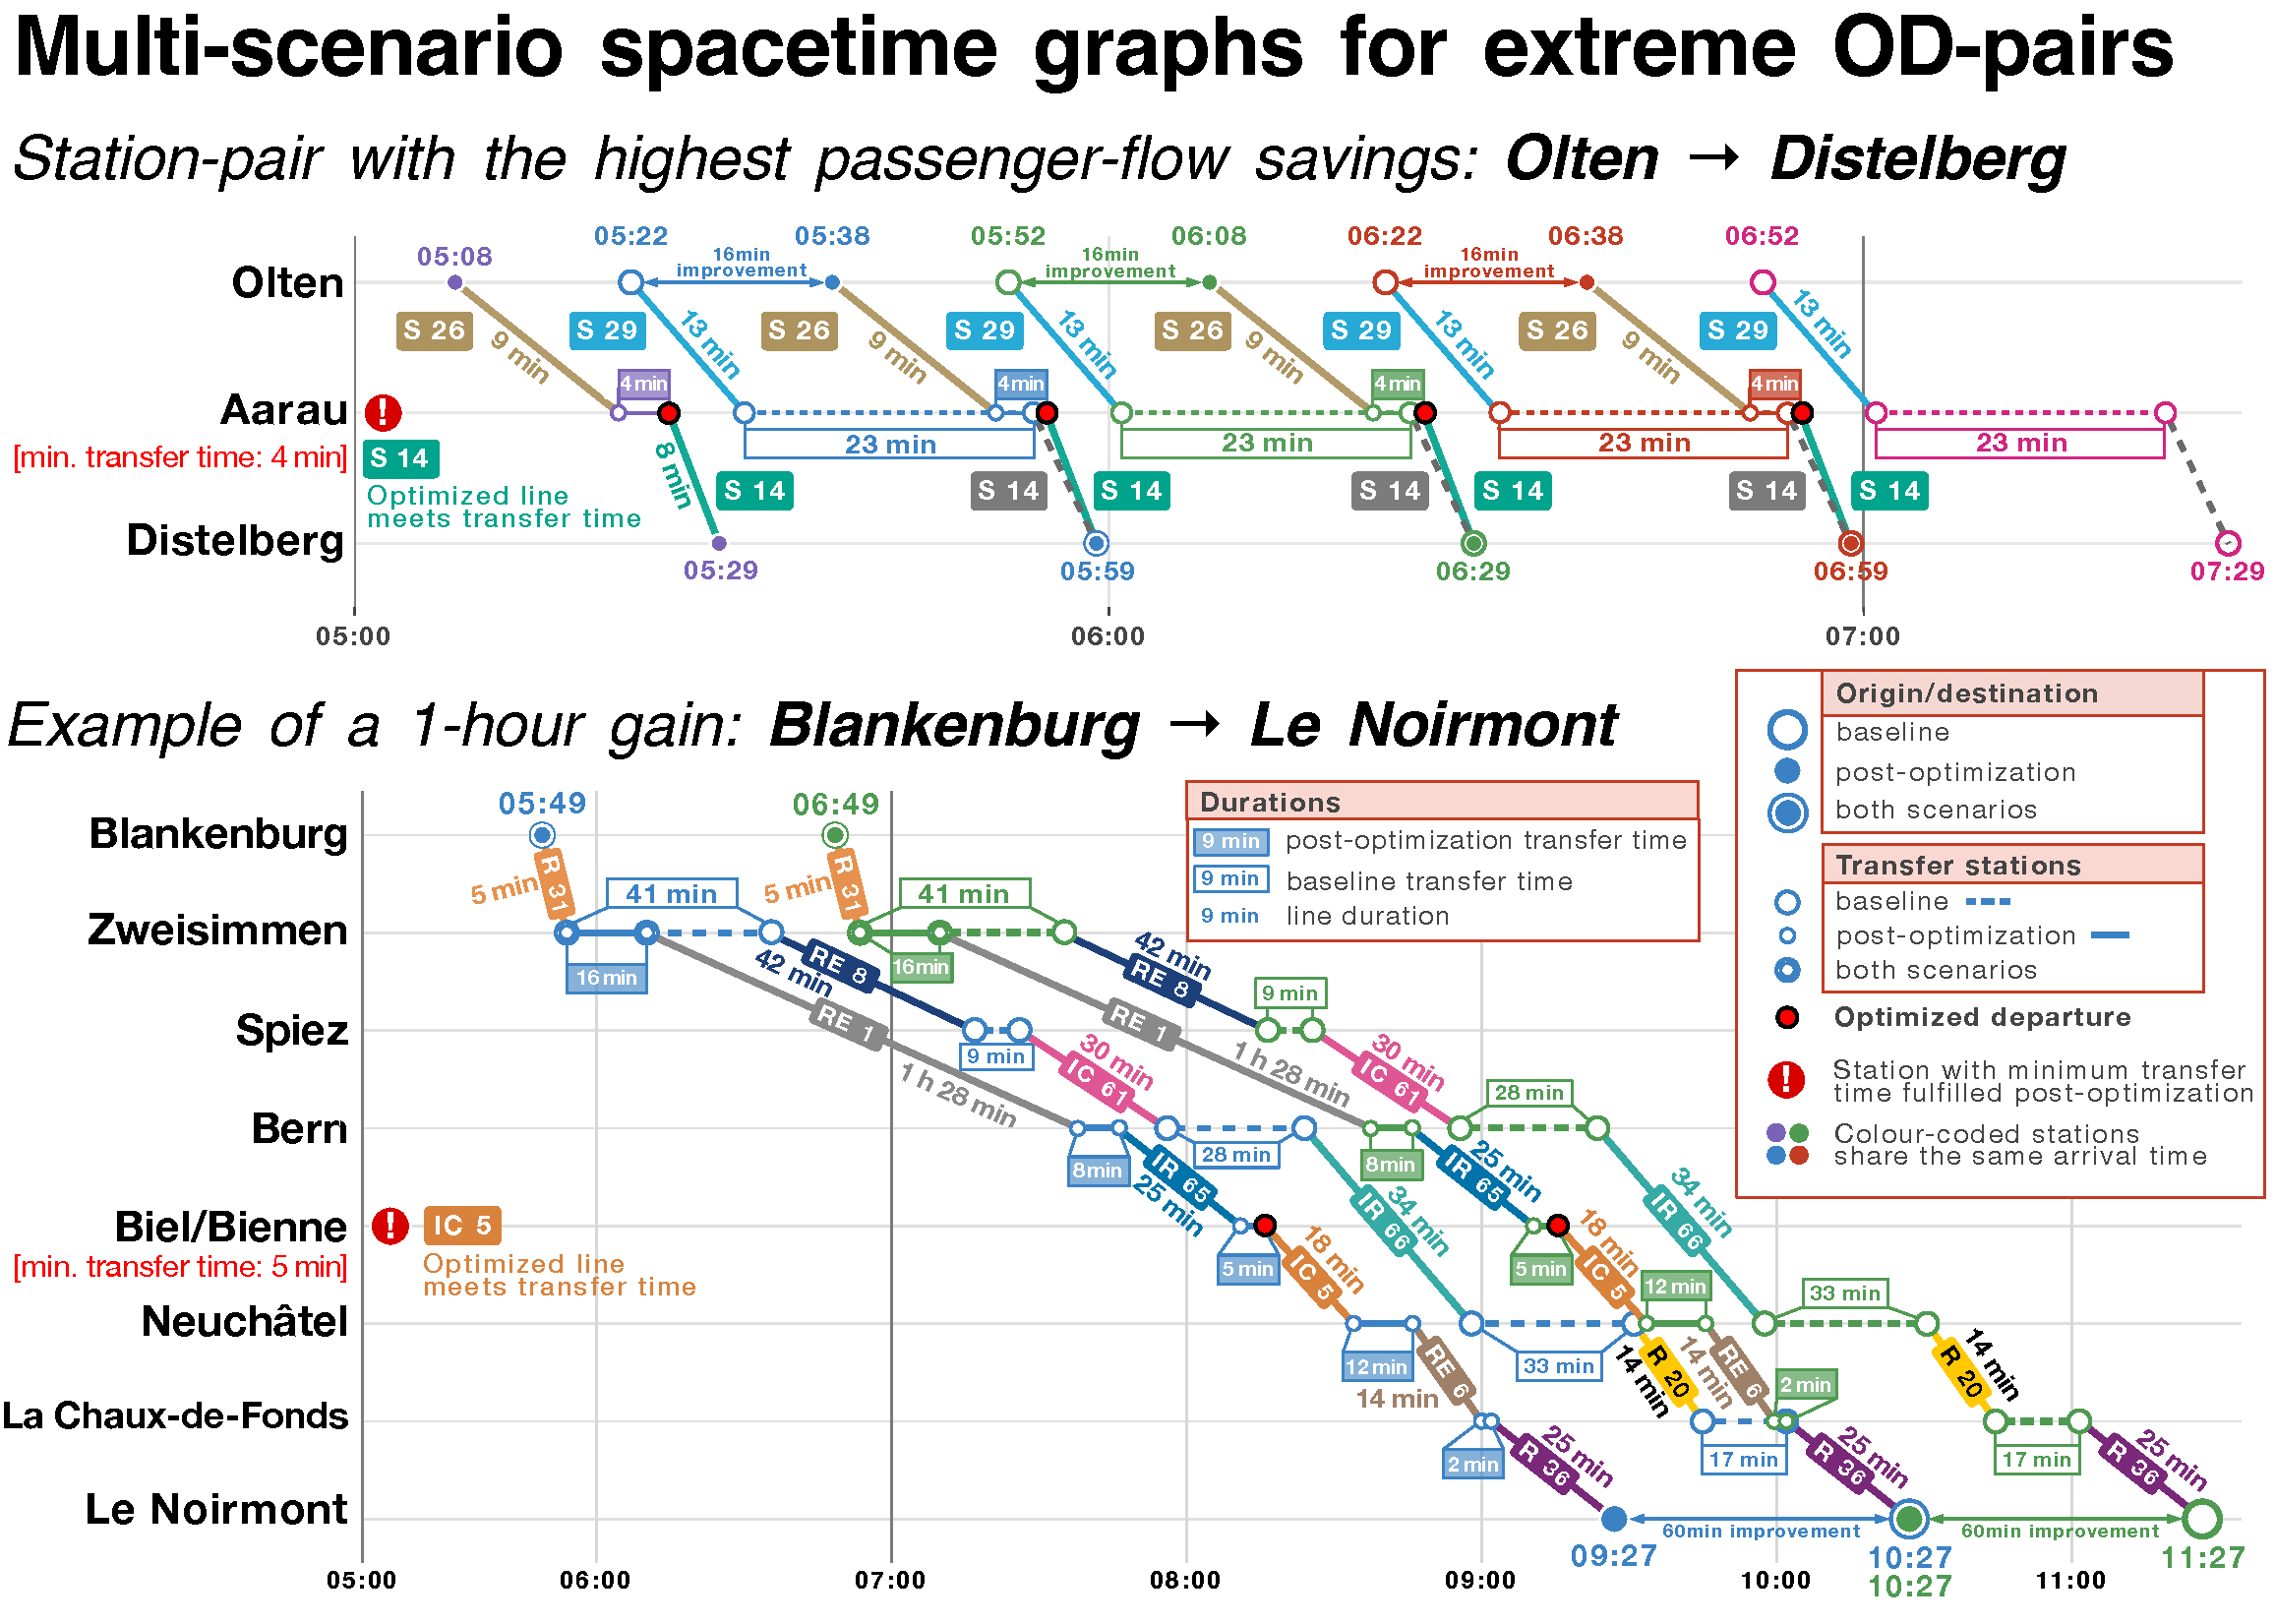
\includegraphics[width=\textwidth]{figures/part-II/part2_od_extreme_paths_step3_2035.pdf}
\caption[Multi-scenario spacetime graphs for extreme OD pairs]{Spacetime diagrams for two 2035 OD pairs, showing overlapping baseline and optimized paths. Colour-coded dots pair each arrival with its departures and allow direct comparison between scenarios. See Appendix for simplified versions of this graph.}

\label{fig:part2-od_spacetime_graph}
\end{figure}
Figure~\ref{fig:part2-od_spacetime_graph} shows these last two described 2035 improvements in a 05:00--07:00 origin-departure window. Olten--Distelberg improves because the Aarau transfer wait is adjusted from 3 to 4 minutes, fulfilling the minimum transfer time of a more efficient line pair. Blankenburg--Le Noirmont improves because the baseline route through Bern and Neuchâtel is replaced by a time-saving geographical diversion to Biel/Bienne, made possible by an IC~5 retiming that satisfies the minimum transfer time at Biel/Bienne. The figure therefore illustrates two improvement types: high-demand local transfer gains, and very low-demand cross-country pairs that move up the arrival time by a full hour. These examples clarify why the optimization is evaluated through the full-network passenger-minute objective. The same accepted retiming can shorten a high-value transfer for one set of OD pairs, leave many pairs unchanged, and worsen a small subset. The OD-pair extremes reveal a range of different improvement types concealed by the aggregate result.


\subsection{Spatial pattern by origin}\label{sec:results-part2-spatial}
The spatial analysis follows the origin-side aggregation convention in Equation~\eqref{eq:part1-group-weighted-mean}, applied to the Part~II scenario weights defined in Section~\ref{sec:methods-part2-spatial-outputs}. A value for a canton or municipality therefore describes trips starting in that origin group, not necessarily timetable edits physically located there. The accepted timetable edits are distributed nationally, and their passenger effects can appear at many origins whose routed paths use the retimed sections. Part~II has a much finer spatial coverage than Part~I, with over a thousand more stations per year. This higher resolution also supports municipality-level breakdowns. The resulting spatial effects are best read in three layers: first, the cantonal component progression in Figure~\ref{fig:part2-canton-progression-components}; second, the component-share movement in Figure~\ref{fig:part2-canton-composition-triangle}; and third, the canton and municipality maps in Figures~\ref{fig:part2-canton-origin-delta-maps} and~\ref{fig:part2-municipality-origin-delta-maps}.


\begin{figure}[htb]
\centering
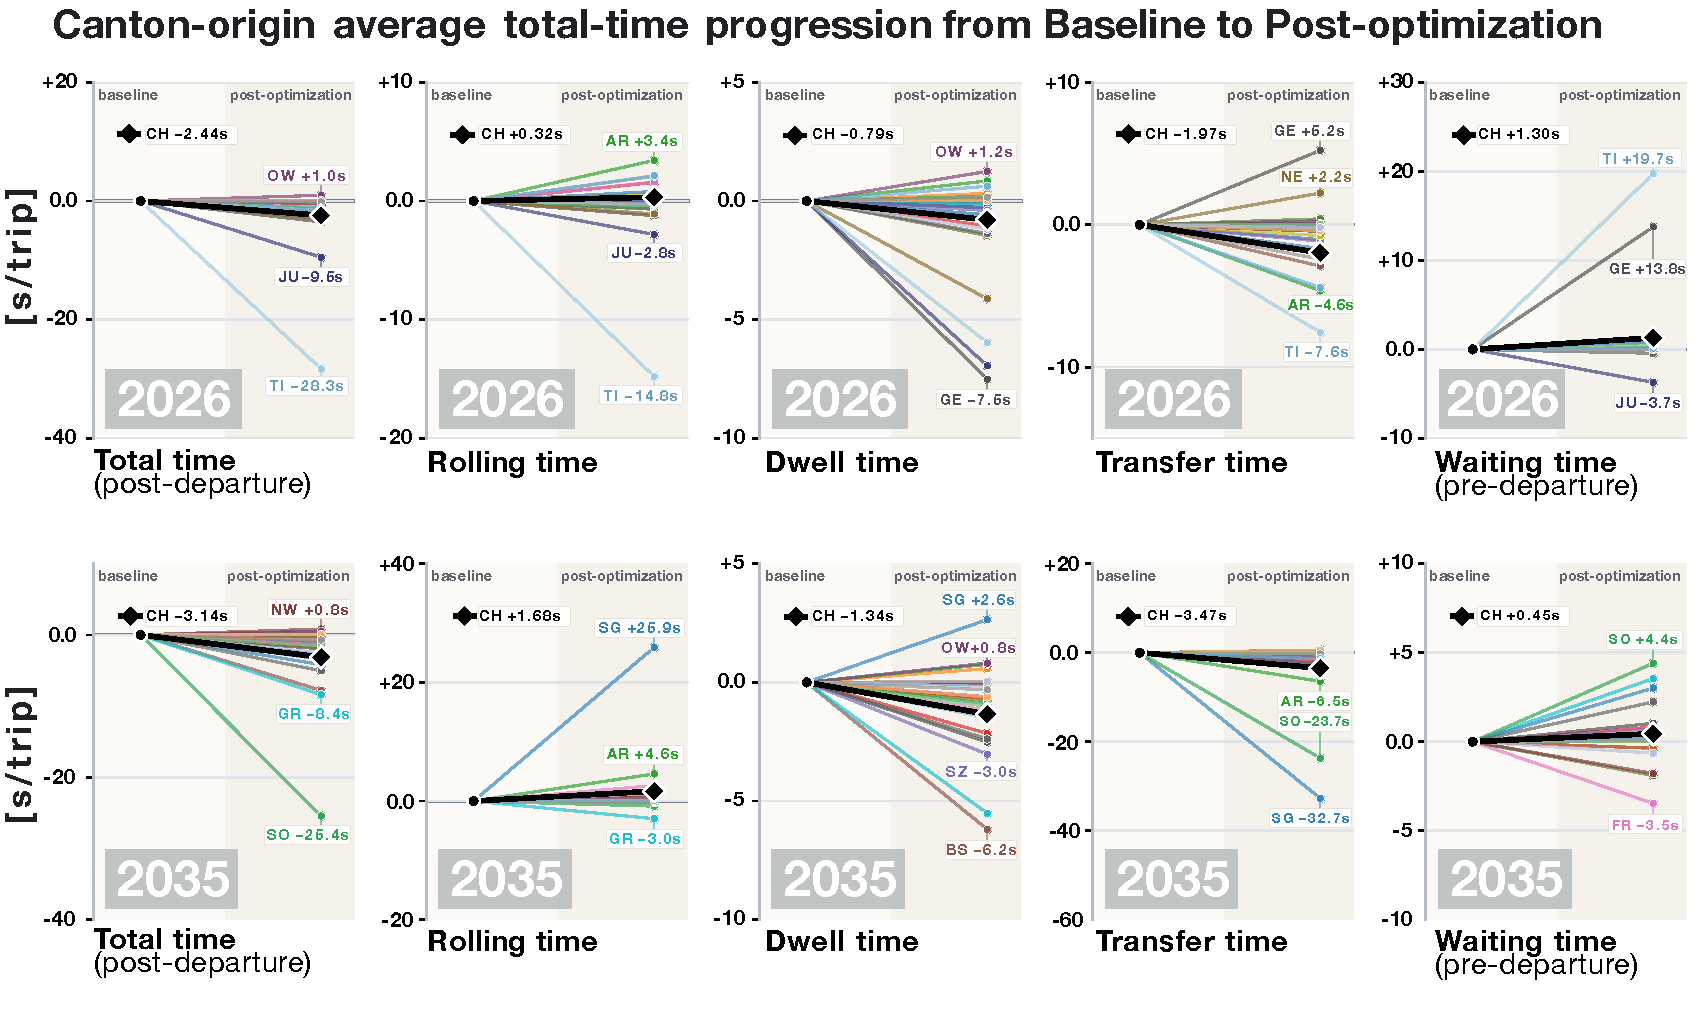
\includegraphics[width=\textwidth]{figures/part-II/part2_canton_progression_by_component.pdf}
\caption[Cantonal travel time component changes]{Cantonal origin progression from Baseline to Optimized Step~3. For each metric, the left column of the pair fixes the baseline reference at zero and the right column shows the Step~3 change in seconds per trip. Negative values indicate lower post-optimized time. In black is the Swiss weighted average, coloured lines are origin cantons.}

\label{fig:part2-canton-progression-components}
\end{figure}

Figure~\ref{fig:part2-canton-progression-components} shows that the optimized results arise from different component changes across origin cantons. Ticino is the clearest 2026 outlier: its average post-departure travel time falls by 28.3 seconds per trip, comprising reductions of 14.8 seconds in rolling time, 6.0 seconds in dwell time, and 7.6 seconds in transfer time. Initial waiting simultaneously rises by 19.7 seconds. This indicates that the substantially faster retained journeys from Ticino are accompanied by less favourable departure spacing rather than improvement in every journey component. In 2035, Solothurn records the largest total reduction, at 25.4 seconds per trip, of which 23.7 seconds is attributable to lower transfer time. St.~Gallen displays a more revealing component trade-off: transfer time falls by 32.7 seconds, while rolling and dwell time rise by 25.9 and 2.6 seconds, respectively, leaving a net post-departure improvement of 4.2 seconds per trip. Because the accepted section shifts preserve physical running times, the higher aggregate rolling time in St.~Gallen reflects a beneficial trade-off in the retained paths used by passengers: longer movement is more than compensated by shorter interchange time.

\begin{figure}[htb]
\centering
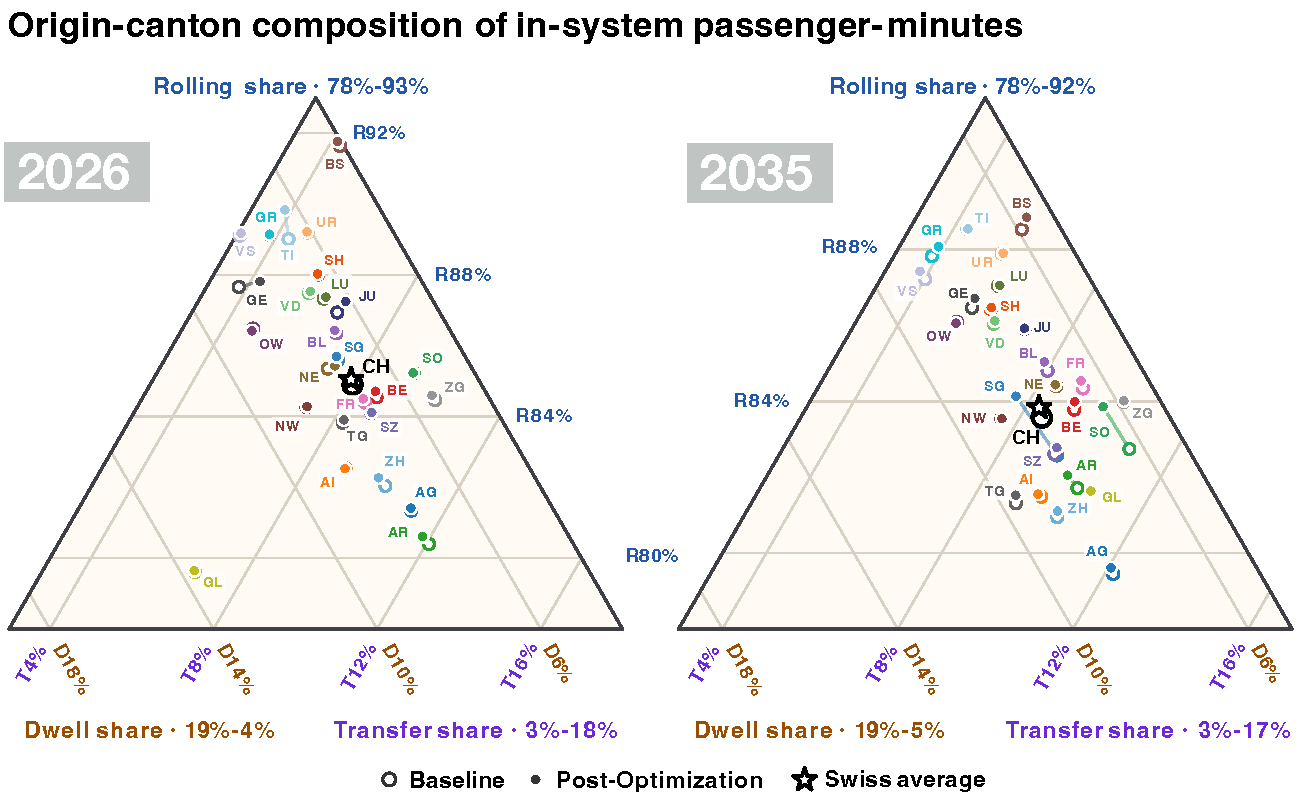
\includegraphics[width=0.95\textwidth]{figures/part-II/part2_canton_composition_triangle.pdf}
\caption[Cantonal travel-time composition]{Origin-canton rolling, dwell, and transfer composition in Baseline and Optimized Step~3. Each point is one Swiss origin canton, weighted by fixed OD demand.}

\label{fig:part2-canton-composition-triangle}
\end{figure}

Figure~\ref{fig:part2-canton-composition-triangle} complements the absolute rolling, dwell, and transfer changes above by showing their shares of each origin canton's post-departure passenger-minutes. A position further up the triangle indicates a more efficient composition, in which a larger proportion of post-departure time is spent moving and less is lost to dwell and transfer time; it does not, however, imply shorter average journeys. The cantons occupy distinctly different positions even before optimization. In 2026, Glarus has the lowest rolling share, at 79.6\%, together with a comparatively high dwell share of 13.6\%, placing it furthest from the rolling-time apex. Basel-Stadt lies at the opposite extreme: rolling accounts for 91.8\% after optimization, the highest share in 2026, and it remains the most compositionally efficient canton in 2035 with a rolling share of 88.9\%. For most cantons, the baseline and post-optimization markers almost overlap, indicating that the optimization does not typically change their overall proportional composition. The clearest upward movements occur in 2035. St.~Gallen's rolling share rises from 82.6\% to 84.1\%, while its transfer share falls from 9.3\% to 7.6\%; Solothurn and Appenzell Ausserrhoden move in the same direction at a smaller scale, as do Ticino and Geneva in 2026. These selected shifts show where optimization reduces the proportion of time absorbed by interchange.



Figures~\ref{fig:part2-canton-origin-delta-maps} and~\ref{fig:part2-municipality-origin-delta-maps} display the origin-group effects of the optimization for cantons and municipalities, respectively. Blue areas indicate lower passenger-weighted post-departure time, red areas indicate higher time, and areas within \(\pm120\)~ms per trip are mapped as unchanged. At the canton level, the 2026 result is geographically broad but varies considerably in magnitude. Twenty-two cantons improve, whereas only Obwalden worsens beyond the neutral threshold. Ticino has by far the largest reduction at 28.3 seconds per origin trip, followed by Jura at 9.5 seconds and Geneva at 3.5 seconds. The strong Ticino result is due to the high-passenger-flow accepted changes around Bellinzona--Giubiasco, while the Geneva improvement coexists with a small cluster of worsened origins within the canton originating north of the main station. In the 2035 map, nineteen cantons improve, led by Solothurn at 25.4 seconds per origin trip, followed by Graubünden and Basel-Stadt at around 8 seconds. The three worsened cantons are confined to central Switzerland: Nidwalden, Obwalden, and Lucerne increase by 0.8, 0.5, and 0.3 seconds per trip, respectively.



\begin{figure}[htb]
\centering
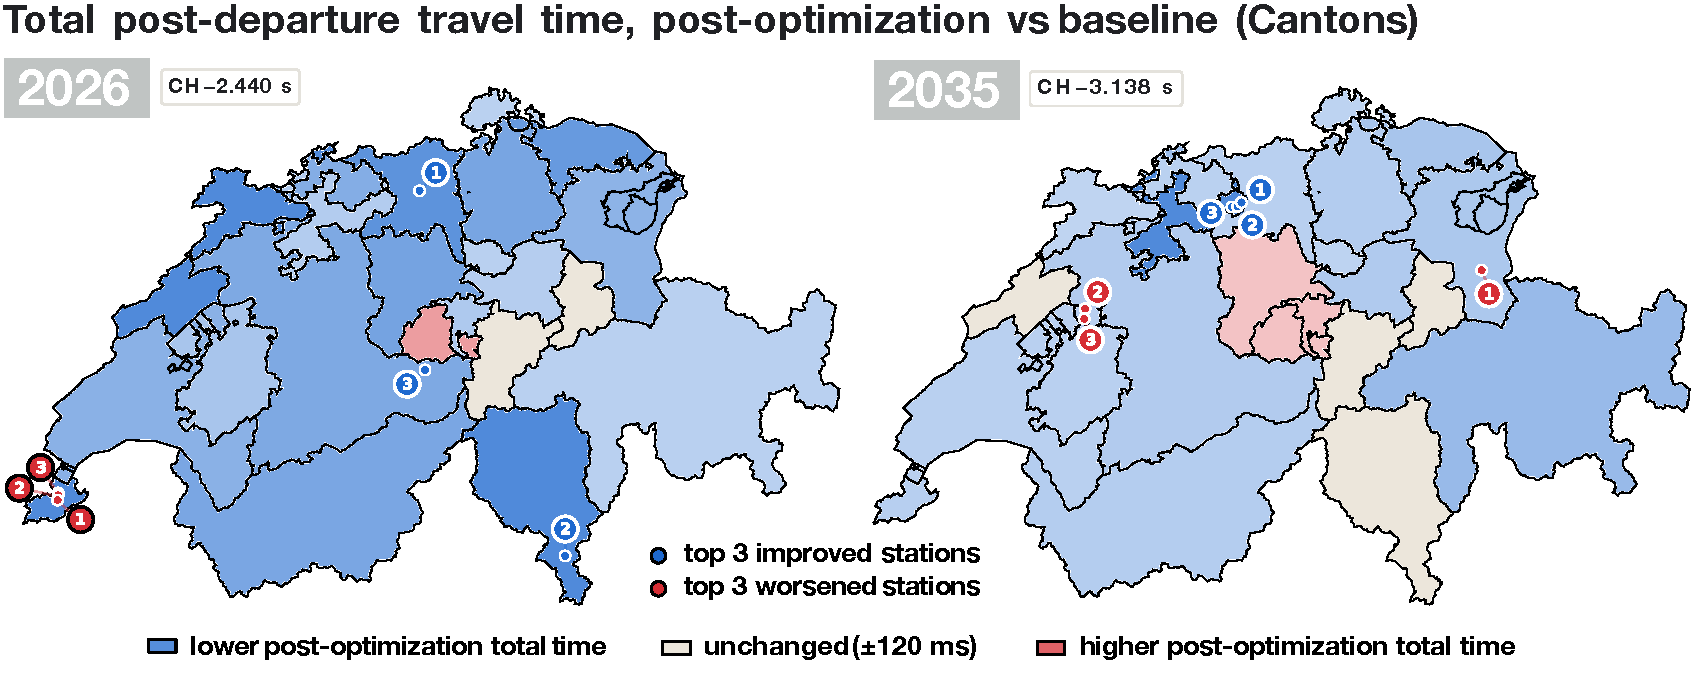
\includegraphics[width=\textwidth]{figures/part-II/part2_step3_vs_baseline_canton_origin_maps.pdf}
\caption[Canton-level origin effects]{Canton-level yearly origin maps. Colours show the passenger-weighted mean in-system total-time change for trips starting in each canton. Blue indicates lower Step~3 time and red indicates higher Step~3 time. Numbered station markers show the most improved/worsened station origins.}

\label{fig:part2-canton-origin-delta-maps}
\end{figure}



\begin{figure}[htb]
\centering
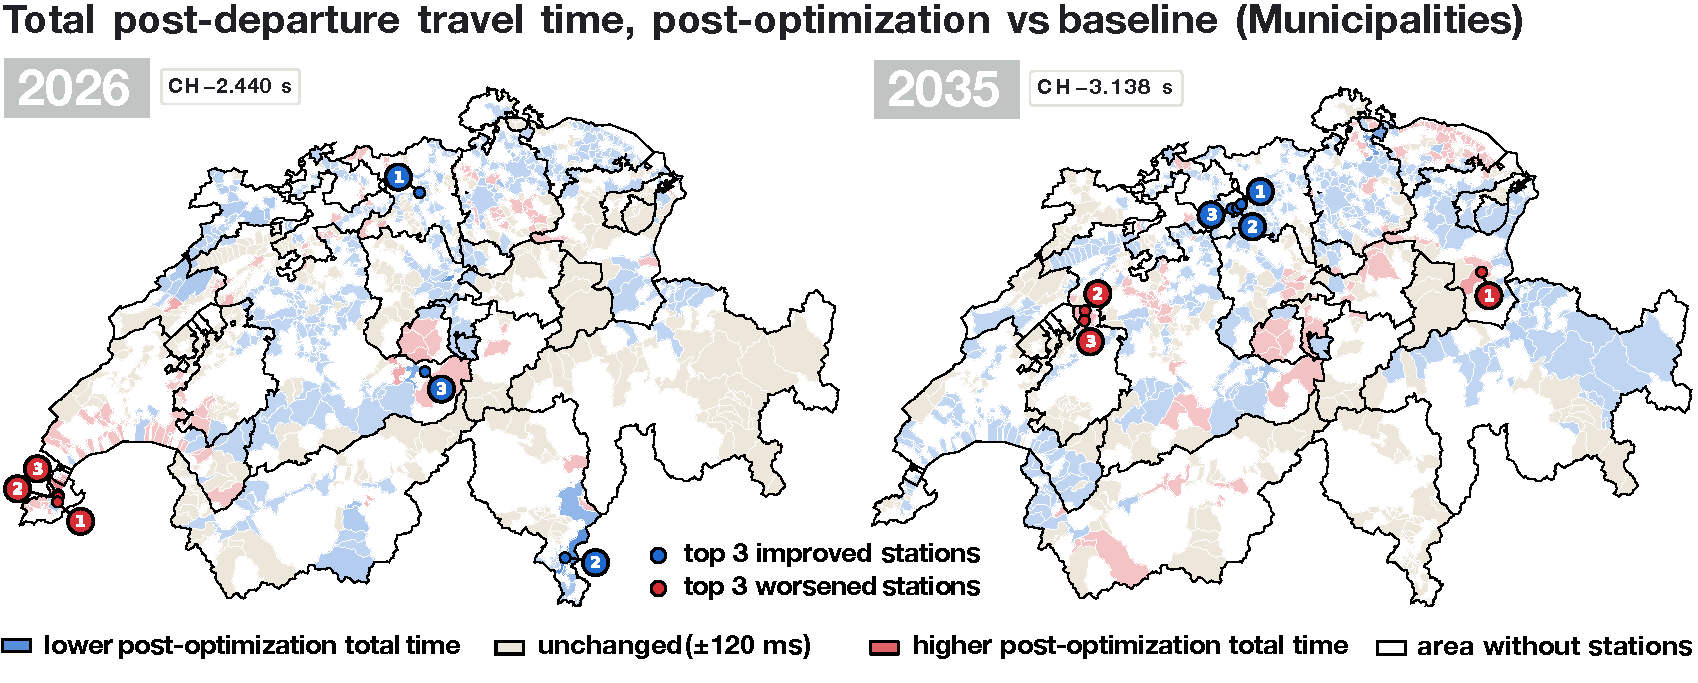
\includegraphics[width=1\textwidth]{figures/part-II/part2_step3_vs_baseline_municipality_origin_maps.pdf}
\caption[Municipality-level origin effects]{Municipality-level yearly origin maps. Colours show the passenger-weighted mean in-system total-time change for trips starting in each municipality. Blue indicates lower Step~3 time and red indicates higher Step~3 time. Numbered station markers show the most improved/worsened station origins.}
\label{fig:part2-municipality-origin-delta-maps}
\end{figure}

The municipality map shows additional intra-cantonal variation. In 2026, the most improved municipalities are far apart: Möriken-Wildegg improves by 84.5 seconds per origin trip, Lugano by 74.5 seconds, and Meiringen by 46.7 seconds. By contrast, the strongest increases form a compact chain along the Geneva lakeshore. Pregny-Chambésy, Bellevue, and Genthod worsen by 61.7, 59.2, and 55.7 seconds per trip, respectively. Municipality and station results partly overlap because around half of the represented municipalities contain only one modelled station. In 2035, the dominant improvement is a tightly defined corridor in the canton of Solothurn: Schönenwerd, Däniken, and Dulliken improve by 3.51, 2.98, and 2.80 minutes per trip. The largest municipal deterioration is more isolated, with Flums increasing by 1.10 minutes; smaller concentrations appear around Mont-Vully and Murten. Table~\ref{tab:part2-spatial-delta-counts} counts improved, unchanged, and worsened origin groups in both maps. Table~\ref{tab:part2-spatial-extremes-levels} then reports the three largest improvements and deteriorations at canton and municipality level.

\clearpage

\begin{table}[htb]
\centering
\caption[Counts of changed origin groups]{Origin groups improved, unchanged, and worsened after Optimized Step~3 relative to Baseline. The unchanged band is \(\pm120\) ms per trip. Negative total-time changes are counted as improvements.}
\renewcommand{\arraystretch}{0.78}
\label{tab:part2-spatial-delta-counts}
\resizebox{0.7\textwidth}{!}{%
\begin{tabular}{llrrrr}
\toprule
\textbf{Year} & \textbf{Origin grouping} & \textbf{Groups} & \textbf{Improved} & \textbf{Unchanged} & \textbf{Worsened} \\
\midrule
2026 & Canton & 26 & 22 & 3 & 1 \\
2026 & Municipality & 853 & 370 & 361 & 122 \\
2026 & Station & 1'592 & 642 & 739 & 211 \\
\midrule
2035 & Canton & 26 & 19 & 4 & 3 \\
2035 & Municipality & 847 & 441 & 295 & 111 \\
2035 & Station & 1'579 & 811 & 572 & 196 \\
\bottomrule
\end{tabular}%
}
\end{table}
\begin{table}[htb]
\centering
\small
\setlength{\tabcolsep}{3.8pt}
\renewcommand{\arraystretch}{0.85}

\caption[Largest canton and municipality effects]{Largest canton- and municipality-origin total-time changes relative to the baseline. Values are passenger-weighted mean seconds per trip for trips starting in the listed origin group. Negative values indicate lower total time in Optimized Step~3. Station-origin extremes are shown separately in Figure~\ref{fig:part2-station-extremes}.}


\label{tab:part2-spatial-extremes-levels}
\resizebox{0.86\textwidth}{!}{%
\begin{tabular}{c l c l r l r}
\toprule
\textbf{Year} & \textbf{Origin grouping} & \textbf{Rank} & \textbf{Most improved} & \textbf{[s/trip]} & \textbf{Most worsened} & \textbf{[s/trip]} \\
\midrule
2026 & Canton & 1 & Ticino & -28.3 & Obwalden & 1.0 \\
2026 & Canton & 2 & Jura & -9.5 & Uri & 0.1 \\
2026 & Canton & 3 & Genève & -3.5 & Appenzell-Innerrhoden & 0.1 \\
\midrule
2026 & Municipality & 1 & Möriken-Wildegg & -84.5 & Pregny-Chambésy & 61.7 \\
2026 & Municipality & 2 & Lugano & -74.5 & Bellevue & 59.2 \\
2026 & Municipality & 3 & Meiringen & -46.7 & Genthod & 55.7 \\
\midrule\midrule
2035 & Canton & 1 & Solothurn & -25.4 & Nidwalden & 0.8 \\
2035 & Canton & 2 & Graubünden & -8.4 & Obwalden & 0.5 \\
2035 & Canton & 3 & Basel-Stadt & -7.8 & Luzern & 0.3 \\
\midrule
2035 & Municipality & 1 & Schönenwerd & -210.7 & Flums & 66.1 \\
2035 & Municipality & 2 & Däniken & -178.8 & Mont-Vully & 31.2 \\
2035 & Municipality & 3 & Dulliken & -167.7 & Murten & 25.6 \\
\bottomrule
\end{tabular}
}
\end{table}

Station origins are presented in Figure~\ref{fig:part2-station-extremes}, which displays the five most improved and worsened stations in each year, the top three of which are also represented by the numbered markers in Figures~\ref{fig:part2-canton-origin-delta-maps} and~\ref{fig:part2-municipality-origin-delta-maps}. Overall, the spatial result is shown to vary substantially. The nature of the accepted timetable edits leads to spread-out localized benefits and costs, and certain regions may run counter to the national trend. The maps and figures in this chapter have made clear where those accepted shifts matter for passengers starting their trips, quantifying the geographic spread of this thesis' optimization by disaggregating the national averages.


\begin{figure}[htb]
\centering
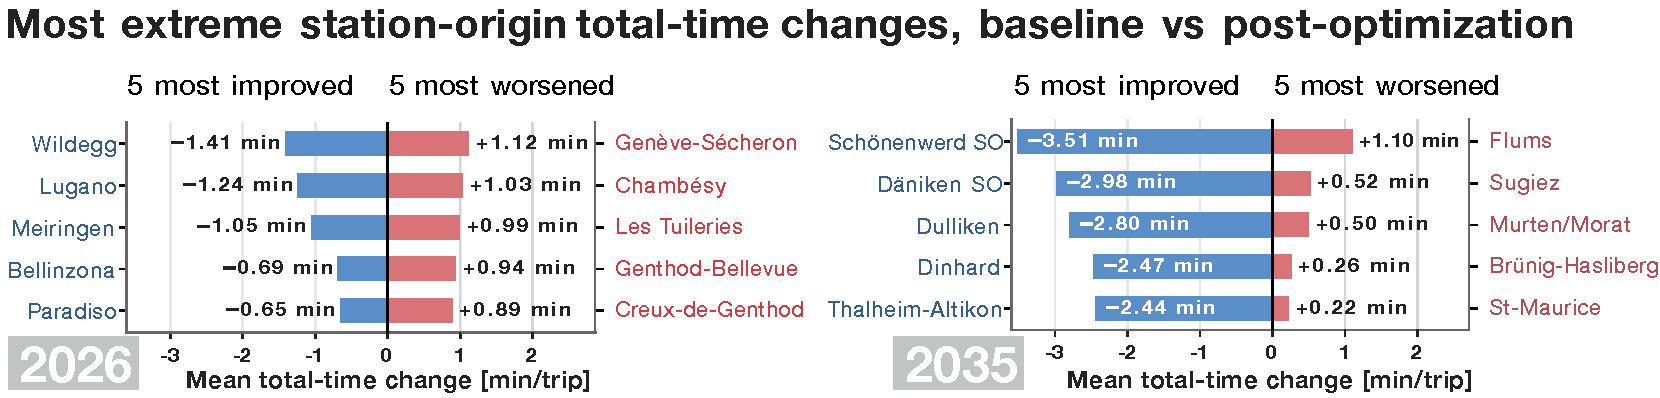
\includegraphics[width=\textwidth]{figures/part-II/part2_station_total_time_extremes.pdf}
\caption[Largest station-origin effects]{Five largest improvements/deteriorations in passenger-weighted mean station-origin total time after Optimized Step~3 relative to Baseline. The mean is taken over all station-origin trips, weighted by the fixed OD demand assigned to each destination. Negative values indicate improvement.}


\label{fig:part2-station-extremes}
\end{figure}
\clearpage


\subsection{Reachability and passenger-load reallocation}\label{sec:results-part2-reachability-loads}
Figure~\ref{fig:part2-reachability-top-origins} compares the origin stations that benefit most from Step~3 in two different ways. The upper panels rank origins by the passenger-minutes saved each day across all destinations reached more quickly. The lower panels instead rank them by the number of faster destinations, irrespective of how many passengers use those individual OD pairs or how large each saving is. The values in parentheses provide the other measure for the same origin, making it possible to distinguish improvements that are concentrated on a few high-value OD pairs from those that extend more broadly across the network. This origin-level view complements the OD histogram in Figure~\ref{fig:part2-histogram2}: changed OD pairs account for only a small portion of the national distribution, but comparable passenger-minute benefits can arise either from large improvements on low-flow links or from small improvements on high-flow links.

\begin{figure}[H]
\centering
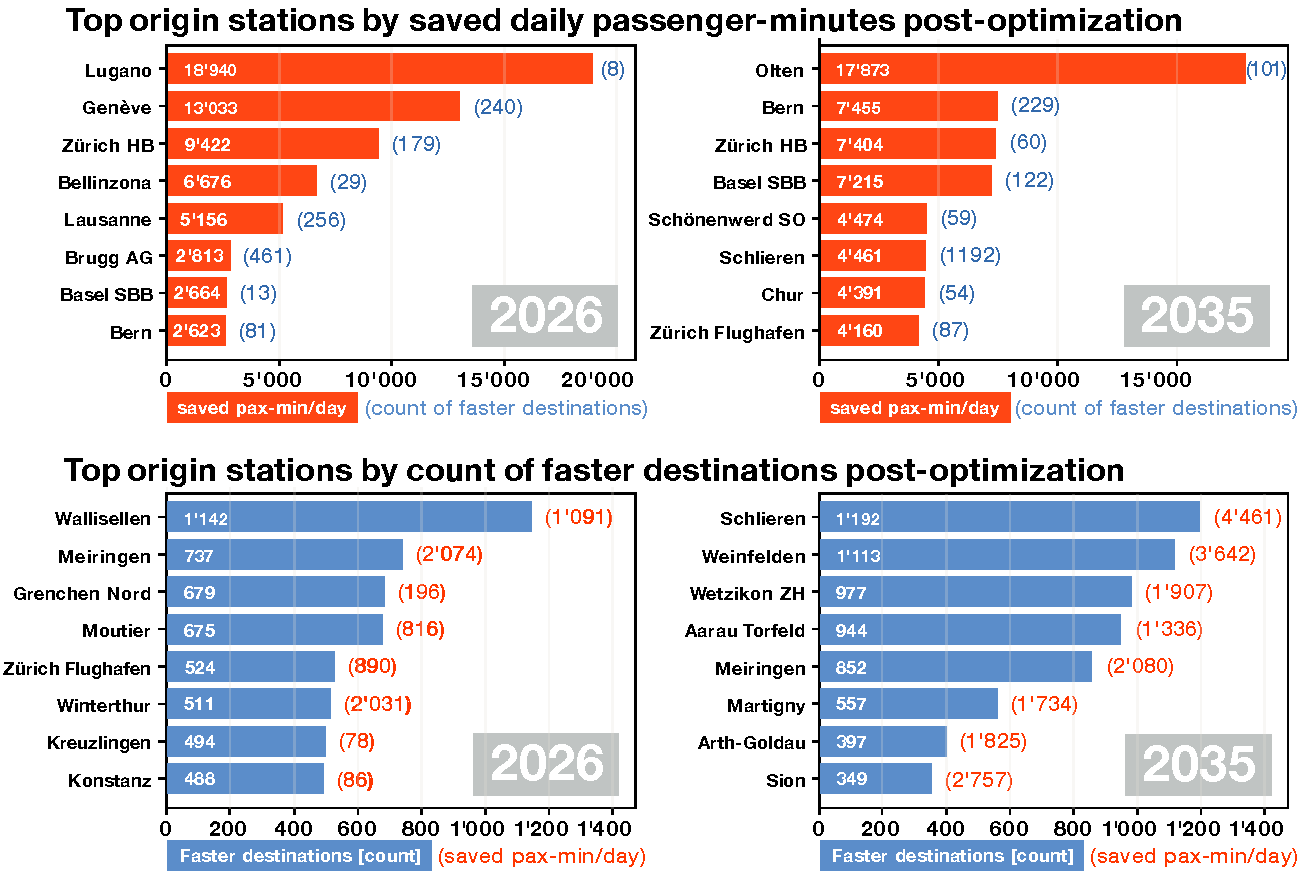
\includegraphics[width=0.85\textwidth]{figures/part-II/part2_top_origins.pdf}
\caption[Leading origins by reachability and savings]{Top optimized origin-stations, ranked separately by daily passenger-minute savings and by the number of faster-to-reach destinations. Parenthetical labels report the complementary measure, allowing broad but shallow improvements to be distinguished from concentrated, demand-intensive gains.}
\label{fig:part2-reachability-top-origins}
\end{figure}

The two rankings produce different sets of leaders. In 2026, Wallisellen reaches 1'142 destinations more quickly but saves only 1'091 passenger-minutes per day, indicating a wide set of relatively small or lightly weighted improvements. Lugano presents the opposite pattern: only eight destinations become faster, yet they generate 18'940 saved passenger-minutes per day. Its benefit is therefore concentrated on a small number of heavily used or substantially improved OD pairs. In 2035, Schlieren leads with 1'192 faster destinations and 4'461 saved passenger-minutes, whereas Olten leads by passenger impact, saving 17'873 passenger-minutes across 101 destinations. The optimization can therefore have substantial network reach without producing the largest aggregate passenger benefit at the same origin. Figure~\ref{fig:part2-schlieren-reachability} shows what Schlieren's broad improvement looks like geographically. Both panels map the fastest observed 2035 travel time from Schlieren to every other Swiss station; the colours represent isochronic travel-time bands. In the post-optimization map, stations with an internal white dot mark destinations reached faster than in the baseline. These stations are those that require a transfer in Zürich Altstetten, and therefore permit departing one minute later due to the timetable edit of S-Bahn line ``H'' in Table~\ref{tab:part2-accepted-edits-2035}. Almost all of the 1'192 marked destinations are reached exactly one minute sooner, while the remaining destinations are unchanged. Across all demand-weighted trips leaving Schlieren, including unchanged destinations, this corresponds to an average saving of 39.7 seconds per trip. The result demonstrates how a retiming encountered early in a journey can propagate to distant destinations. Schlieren has approximately 12 times as many faster destinations as Olten (1'192 compared with 101), but its 4'461 saved passenger-minutes per day are approximately one quarter of Olten's 17'873. Geographic breadth and passenger impact are therefore related but distinct outcomes.



\begin{figure}[H]
\centering
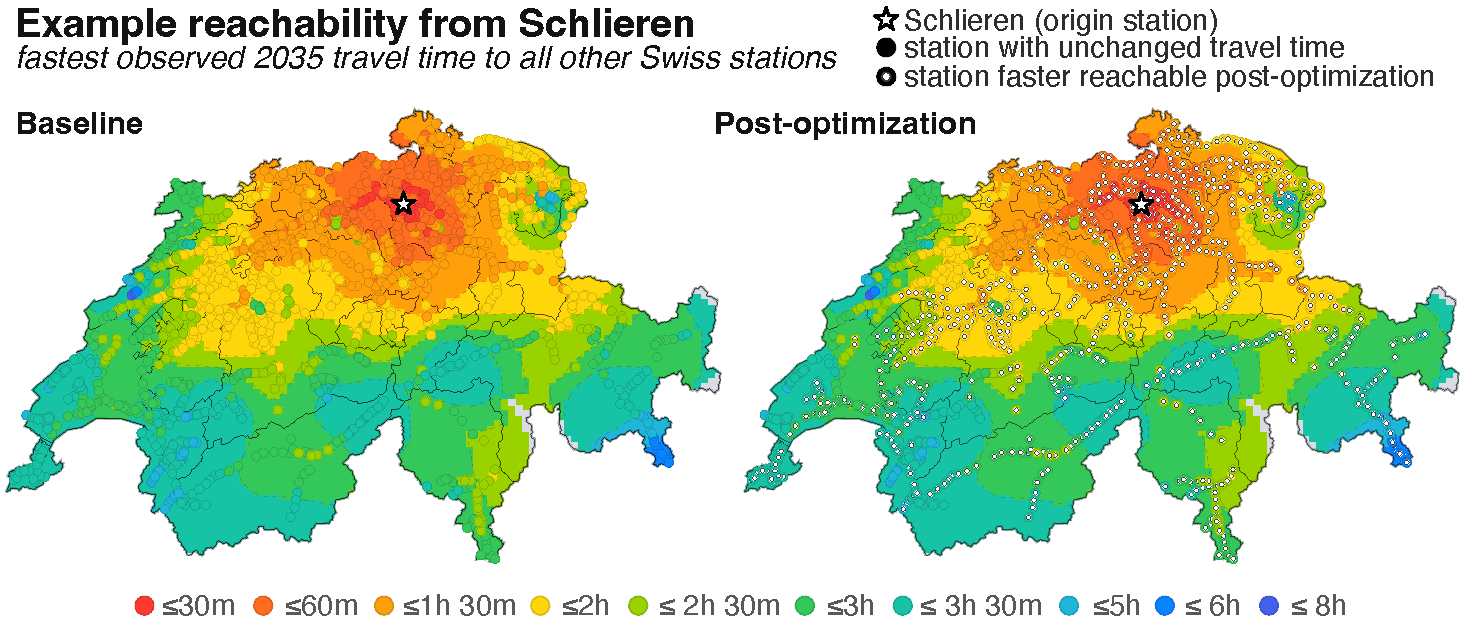
\includegraphics[width=\textwidth]{figures/part-II/part2_schlieren_reachability_2035.pdf}
\caption[Reachability from Schlieren in 2035]{Fastest post-departure travel times from Schlieren to other Swiss stations in 2035. Colours show isochronic travel-time bands. Stations with white dots are faster-to-reach than in the baseline.}
\label{fig:part2-schlieren-reachability}
\end{figure}
\begin{figure}[H]
\centering
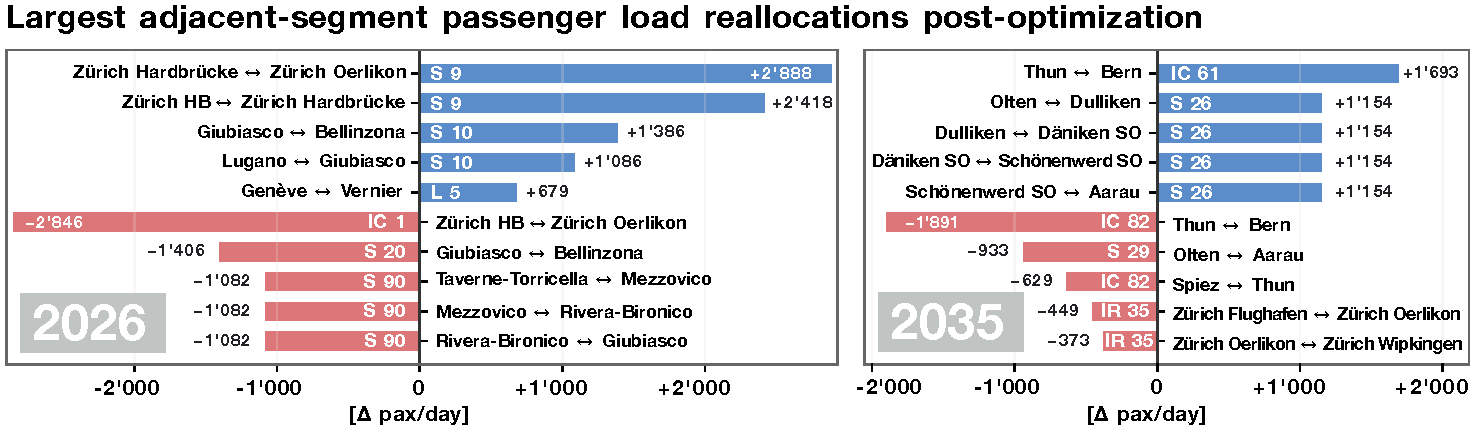
\includegraphics[width=\textwidth]{figures/part-II/part2_segment_load_changes.pdf}
\caption[Largest adjacent-segment load reallocations]{Largest adjacent station segment line reallocations by daily passenger load.}

\label{fig:part2-segment-load-changes}
\end{figure}
Figure~\ref{fig:part2-segment-load-changes} shows the largest changes in daily passenger load on adjacent station segments. Blue bars identify segments receiving more path-allocated passengers after optimization, while red bars identify segments receiving fewer. Because OD demand is fixed, these changes represent reassignment between available paths rather than additional ridership.

The paired increases and decreases reveal several apparent substitutions. In 2026, IC~1 between Zürich HB and Zürich Oerlikon loses 2'846 passengers per day, while the S~9 through Zürich Hardbrücke gains 2'418 passengers on its first segment and 2'888 on its second. In Ticino, the S~10 gains 1'386 passengers between Giubiasco and Bellinzona at the expense of the S~20, helping to explain the concentrated passenger-minute savings at Lugano and Bellinzona in Figure~\ref{fig:part2-reachability-top-origins}. In 2035, the Thun--Bern allocation shifts from IC~82, which loses 1'891 passengers per day, to IC~61, which gains 1'693. A second substitution occurs between Olten and Aarau, from the S~29 to the S~26, corresponding spatially to the improvements around Olten and the Solothurn municipalities identified in the preceding subsection.

\clearpage




\clearpage
\section{Discussion II}\label{sec:DiscussionII}

\subsection{From timetable analysis to timetable alteration}\label{sec:discussion-part2-throughline}

Part~II evolves the diagnostic framework of Part~I into an intervention framework. Part~I established that timetable quality can be effectively analysed when complete journeys are weighted by passenger demand and decomposed into rolling, same-train dwell, transfer, and initial waiting time. It also demonstrated that the large historical improvement of the Swiss timetable was spatially uneven. Part~II retains the same journey components and dominance-based path logic, but moves on to the second research question. With demand fixed within 2026 and 2035, it asks whether specific timing relationships can be improved without changing line patterns or section running times.

Part~II's higher resolution improves the causal clarity of the analysis. The station universe expands from 131 stations in Part~I to nearly 1'600 stations, including essentially all major and minor Swiss stations and non-rush-hour periodic services. Every scenario within a model year uses the same OD matrix, so measured differences arise from timetable timing, path retention, and dominance-share reallocation rather than from changes in demand composition. Retiming candidates are also evaluated beyond the sections where they are applied: each completed timetable is rebuilt across the full OD system, allowing a local transfer adjustment to affect every downstream journey that uses it.

The final Step~3 timetable reduces the full-network objective by 94'216 passenger-minutes per day in 2026 and 112'419 in 2035, equivalent to 2.78 and 3.12 seconds across all trips — or 73.9 and 83.0 seconds if only considering actually affected pairs. These national means are small relative to the historical gains in Part~I, as expected for minute-scale refinements of an already coordinated timetable. They nevertheless represent substantial savings for specific OD pairs. Only 3.76\% of positive-demand OD pairs change at all in 2026 and 3.38\% in 2035, but this changed set includes repeated high-flow connections and origins with improvements measured in tens of seconds or several minutes per trip. Deteriorations are fewer and generally smaller than the improvements.


\subsection{Contribution of the three optimization steps}\label{sec:discussion-part2-steps}

The three steps make complementary contributions, with each stage refining the evidence used for selection. Step~1 uses station-board transfer flows and near-miss proxies to identify straightforward local retiming opportunities, saving 13'699 passenger-minutes per day in 2026 and 54'210 in 2035. Step~2 evaluates additional hub-subgraph-derived candidates against exact paths retained under the validated Step~1 timetable. Its marginal contribution is smaller, saving 10'278 passenger-minutes per day in 2026 and 11'803 in 2035. Step~3 provides most of the 2026 saving and a large share of the 2035 saving. Its lower transfer-context threshold, broader candidate pool, and repeated marginal rescoring identify improvements omitted by the earlier hub-focused search, adding 70'239 passenger-minutes per day in 2026 and 46'407 in 2035. Proxy scores remain useful for narrowing the search, while the rebuilt full-network objective is decisive for the final scenario, leading to two reversals in Step~3. After these reversals, 42 edit rows remain active in 2026 and 37 in 2035.

\newpage
\subsection{Travel time components and spatial concentration}\label{sec:discussion-part2-mechanisms}

Transfer and same-train dwell reductions account for most of the final post-optimization saving. In 2026, transfer and dwell passenger-minutes fall by 72'466 and 28'201 per day, respectively, while rolling time rises by 6'451. In 2035, transfer and dwell time fall by 124'488 and 47'962 passenger-minutes, while rolling time rises by 60'030. This pattern follows from a search that retimes transfers and local dwell relationships without changing section running times. Full OD rerouting can nevertheless increase aggregate rolling time when passengers switch to a different route, or when the dominance share assigned to an existing path changes after a transfer becomes feasible or infeasible. A passenger may therefore spend longer moving on board yet arrive earlier because transfer or dwell time falls by more. The component changes are therefore network-allocation effects and do not alter the train's running speed.


The analysed OD examples make this distinction visible. Olten--Distelberg improves through a one-minute shift that turns an infeasible three-minute transfer at Aarau into a feasible four-minute transfer, producing a large passenger-minute gain on a comparatively high-demand relation. Blankenburg--Le Noirmont instead improves by one hour because an IC~5 retiming makes a faster route through Biel/Bienne feasible. The latter has a dramatic per-trip improvement but very little demand; the former is less extreme per trip but more important to the national objective. This is why per-trip minutes and passenger-minutes are reported separately. Initial waiting, defined from the dominance-weighted departure intervals, rises by 31'148 passenger-minutes per day in 2026 and 16'141 in 2035. Small retimings can turn an even 30/30-minute pattern into intervals such as 29/31 minutes, causing this initial wait rise due to dominance patterns, as the optimized objective includes only post-departure travel time. The result therefore favours in-system journey improvements rather than perfectly even departure spacing.

The spatial outputs show why national means are insufficient on their own. Ticino has the strongest 2026 origin-canton improvement, while Solothurn leads in 2035; station and municipality effects are even more varied still. Reachability and passenger-minute rankings reveal different forms of benefit. In 2035, Schlieren reaches 1'192 destinations one minute sooner, approximately 12 times the 101 faster destinations from Olten, yet produces only about one quarter of Olten's passenger-minute saving. The segment-load analysis then connects these origin effects to implied route choice: fixed demand moves between IC and S-Bahn alternatives in Zürich, between S~10 and S~20 in Ticino, and between IC~61/IC~82 and S~26/S~29. A small set of event shifts can therefore affect paths and passenger loads far beyond the edited sections, even though most OD pairs remain unchanged.

\subsection{Suitability of the implemented matheuristic model}\label{sec:discussion-part2-matheuristic}

The workflow is a model-based matheuristic because a mathematically specified passenger-time objective and timetable constraints guide a heuristic search. The global target is to minimize passenger-weighted post-departure time across all positive-demand OD pairs. Candidate selection can be written as a binary linear problem with passenger-minute scores, incompatibility constraints, validation conditions, and step-specific restrictions, while the PESP framework provides the formal reference for periodic event and activity relationships. Exact path calculations, zero-invalidated-flow requirements, combined-set checks, and completed-scenario evaluation provide the model-based components. The implemented method nevertheless generates candidates heuristically and selects them sequentially rather than solving the complete binary formulation with a MILP solver.

The workflow separates iterative candidate selection from full-network scenario evaluation. Completed scenario states contain fully-detailed nondominated OD path descriptions and dominance-based passenger allocation for approximately 2.1 million positive-demand directed OD pairs per model year, but this detailed enrichment is added onto the bare OD matrix after a scenario has been assembled rather than during every candidate-scoring iteration. The Step~3 candidate selection took several hours because it re-scored cached reference paths: 8 hours for 2026 and 5.2 hours for 2035. Complete routing was substantially more demanding. The final Step~3 timetable rebuild for both model years required approximately 133.8 core-hours to run sequentially, or just 14.1 hours using ten parallel processes, before a similar multi-hour demand enrichment passthrough and subsequent analysis stages; the full-scenario build was therefore a computation of around 24 hours. Candidate selection was therefore responsible for approximately half the total required time, with the complete rerouting and validation responsible for the other half.

These runtimes explain why the complete passenger response is evaluated outside the candidate-selection loop. The daily scenario representations comprise 13'293 canonical train-service runs and 292'116 arrival/departure station events in 2026, and 14'990 runs and 314'783 events in 2035, before passenger paths are considered. A fully integrated PESP/MILP pursuing the same objective would have to optimize timetable events jointly with transfer feasibility, retained passenger paths, and dominance-based allocation. For \(n\) stations, the directed OD universe contains \(n(n-1)\) relations and therefore grows quadratically with station coverage; incorporating these relations would create a substantially larger formulation than the timetable-event model alone.


The literature reviewed in Section~\ref{sec:periodic-timetabling} shows why a fully integrated exact formulation is an appealing but demanding alternative. Benders-type approaches can separate timetable decisions from passenger or resource subproblems and can provide bounds, but the demonstrated applications operate at different forms of scale. The Zurich-Luzern-Chur triangle logic-based Benders paper is exact and highly detailed microscopically, but its complexity is concentrated in infrastructure resources, route alternatives, and train conflicts rather than large-scale OD routing \citep{leutwilerCorman2022LogicBenders}. The passenger-oriented Lower Saxony case is closer in objective, but is much smaller in station coverage and still reports a nonzero optimality gap \citep{yaoEtAl2025HybridBenders}. Applying Benders to the present national station-level problem would therefore require a new formulation, especially because timetable edits can change feasible path sets and dominance-based passenger allocation. It remains a promising direction for bounds on reduced or reformulated instances, but the literature review does not show that a complete globally optimal formulation at the scale of Part~II is currently sensible. A model-based matheuristic is used instead to keep the search traceable and computationally feasible.

The alternative would be to keep passenger assignment external and evaluate many trial timetables by repeated full-network routing. This is unsuitable as an inner loop in the present architecture: a complete two-year routing rebuild already requires 14.1 hours before demand enrichment and analysis, so even a modest illustrative search of 1’000 full-network trial states would imply roughly 14’100 hours under the same setup, or more than 1.5 years. Even if incremental filtering or subgraph-limited rerouting could reduce this substantially, the resulting runtime would still be too long under globally-optimal models. Complete national routing is therefore suitable for final scenario validation, but not as a frequently called inner-loop evaluator in the present architecture. The implemented matheuristic preserves national passenger detail and interpretable timetable edits within the available computational budget, while leaving globally bounded integrated formulations as future research.

The matheuristic therefore uses cached reference paths as a selective evaluation layer and reserves full OD rerouting for completed scenarios. This is the central compromise of the architecture. The cached checks make it possible to test many compatible integer-minute section shifts and to account for interactions among accepted edits on retained paths, while the final rebuild captures the broader passenger response, including newly created, removed, or reallocated alternatives. The workflow thus avoids using full national routing as an inner-loop evaluator, but still validates the accepted timetable on the complete station-level passenger network. This evaluation structure gives the method its main practical advantage: traceability. Every accepted or reversed timetable row can be linked to a transfer context, a passenger-minute score, a compatibility decision, and downstream OD effects after the completed-scenario rebuild. The price of this traceability is that the global binary candidate problem is not solved and no optimality bound is produced. The contribution is consequently a fully rerouted and validated improvement at national station-level scale, not a claim to the globally optimal Swiss timetable.

\newpage
\subsection{Limitations and future research implications}\label{sec:discussion-part2-limitations}

The accepted edits remain passenger-weighted timetable hypotheses. Rolling-stock circulation, crew duties, platform occupation, infrastructure capacity, headway conflicts beyond the implemented structural checks, and stochastic delay propagation are outside the model, though not expected to be of great concern due to the extremely limited time-shifts at play -- of mostly one or two minutes. However, an operational assessment might therefore reject or further modify individual edits, even when their scheduled passenger effect is positive. Reliability is especially relevant, as Part~I showed in the discussed example of the controversial 2025 Western-Switzerland retimetabled trip-speed decrease. The added timetable buffer time lengthened many scheduled journeys, but improved punctuality. The deterministic Part~II objective cannot quantify that trade-off, so an integration of this type of model with the effect of potential delays is left for future research.

Demand is also modelled rather than directly observed for every OD pair, because SBB publishes station-throughput data rather than full OD-level demand matrices. The gravity seed, station-throughput constraints, transfer correction, and 2035 accessibility adjustment provide a well-performing weighting layer, but alternative demand matrices might influence the ranking of timetable edit candidates. Holding demand fixed across scenarios within each year is nevertheless appropriate for the comparison undertaken here because it isolates the effect of retiming and rerouting. Despite this, expanding the data used in this thesis to better model the effects of induced demand both within each year, and for improved future projections, would improve the accuracy and precision of the reported passenger-minute values, strengthening the validity of the overall model.

These limitations define the next planning stage. The 42 active 2026 edits and 37 active 2035 edits form a compact set of candidates for capacity, robustness, resource-planning, and expert timetable review. Each edit has already passed a demanding passenger-weighted test: structural validation, sequential compatibility checks, and complete OD rerouting. The result is therefore both a network-level finding and an operationally interpretable shortlist for further investigation by the relevant railway operators, namely SBB, BLS, MGB, TILO and Zentralbahn. In addition to these potential operational checks, future studies would do well to implement an expanded probabilistic transfer model, replacing minimum-transfer cutoffs with connection success probabilities. Benders or related decompositions could provide bounds on reduced or reformulated problems, with the aim to create narrowed-in subproblems through informative cuts, so that only affected OD paths are considered in each subproblem. This would permit the rerouting to be run more often during a candidate search. In the most advanced version, the inclusion of enough additional constraints within an overhauled model may lead to the resulting optimization confirming a global minimum, albeit most likely at the cost of requiring a smaller set of stations.

\clearpage
\section{Conclusion}\label{sec:conclusion}

This thesis establishes a unified passenger-weighted framework for measuring and improving periodic rail timetables. Part~I reconstructs the historical Swiss clockface timetable and converts complete journeys into comparable OD-weighted measures of rolling, same-train dwell, transfer, initial waiting, and total post-departure time. Part~II applies the same journey logic prospectively, expanding the model to nearly 1'600 stations and testing small integer-minute retimings through a three-step model-based matheuristic.

The first research question is answered by the historical reconstruction. Timetable-realized journey conditions can be compared consistently across decades when the timetable, route-choice, and demand-weighting layers are represented explicitly. For the selected 131-station network, passenger-weighted post-departure time falls from 51.60 minutes per trip in 1982 to 39.13 minutes in 2026, while initial waiting falls from 28.51 to 13.53 minutes. Rolling, dwell, transfer, and waiting components all improve over the full period, but the spatial and calendar-window results show that progress is neither monotonic nor uniform. Major infrastructure and timetable recasts create broad gains while also redistributing accessibility, and passenger-weighted conclusions can differ materially from unweighted network averages.

The second research question is answered positively. The final corrected Step~3 timetable reduces full-network post-departure travel by 94'216 passenger-minutes per day in 2026 and 112'419 in 2035, equivalent to 73.9 and 83.0 seconds per affected trip. The gains are produced by 42 edited line timings in 2026 and 37 in 2035, all based on integer-minute section shifts that preserve local rolling times. Transfer and same-train dwell reductions dominate the result, while full rerouting reallocates passengers among retained paths and can increase aggregate rolling time or initial waiting. Only 3.76\% of non-zero-demand OD pairs change in 2026 and 3.38\% in 2035, so the national improvement is generated by a selective set of high-value or geographically extensive effects rather than a uniform shift of all journeys.

Methodologically, the thesis connects two perspectives that are often applied separately: retrospective measurement of timetable-realized accessibility and prospective passenger-oriented periodic timetable improvement. The same path and component representation is used to explain historical timetable development, locate component-specific inefficiencies, and evaluate targeted retimings. Part~II extends the reviewed literature by applying the sizeable scope of all Swiss stations and line services to full OD rerouting, dominance-based passenger allocation, procedurally identified local timetable edits, and extensive post-optimization scenario analyses. The model-based matheuristic is central to this contribution, as it combines a mathematically defined global passenger-time target and formal feasibility structures with the heuristic candidate generation and sequential selection required to make the national problem computationally and interpretively manageable.

The resulting proposed timetable is not a fully-vetted operational implementation plan. Station approach track capacity, platform occupation, robustness, and crew constraints remain outside the model and would require expert review before any practical adoption. What the thesis does establish is a complete evidential chain: from periodic timetable records to routed passenger paths, from passenger paths to weighted national performance indicators, and from those indicators to specific retiming candidates whose effects are validated across the full modelled OD system. The historical analysis shows how Swiss passenger-rail efficiency has evolved, while the optimization analysis shows that even an already highly-coordinated clockface timetable still contains measurable potential for improving passenger journeys through targeted retiming. By linking periodic timetable structure to routed passenger journeys, this thesis shows that national clockface systems can be evaluated not only by the regular services they provide, but by the connections they enable, the paths they shape, and the journeys they make possible.

% -----------------------------------------------------------------------------
% Acronyms and notation
% -----------------------------------------------------------------------------

\clearpage
\setcounter{page}{1}
\renewcommand{\thepage}{A\arabic{page}}
\renewcommand{\theHpage}{A\arabic{page}}
\phantomsection
\section*{Acronyms and Notation}
\label{sec:acronyms-notation}
\addcontentsline{toc}{section}{Acronyms and Notation}

This section defines recurring acronyms and mathematical notation. Symbols are grouped first by the structures shared across the thesis and then by the Part~I and Part~II modelling layers.

\subsection*{Acronyms}
\begin{description}
    \item[ADMM] Alternating direction method of multipliers, a decomposition algorithm that coordinates solutions to linked optimization subproblems.
    \item[ARE] Federal Office for Spatial Development (\textit{Bundesamt für Raumentwicklung}).
    \item[BAV] Federal Office of Transport (\textit{Bundesamt für Verkehr}).
    \item[BFS] Federal Statistical Office (\textit{Bundesamt für Statistik}).
    \item[BLS] Bern--Lötschberg--Simplon Railway (\textit{Bern--Lötschberg--Simplon-Bahn}).
    \item[DTV] Daily traffic volume (\textit{durchschnittlicher Tagesverkehr}); in Part~II, an observed or estimated station-throughput measure.
    \item[IPF] Iterative proportional fitting, used to balance an OD seed matrix to specified marginal totals.
    \item[LP] Linear program, with a linear objective and continuous variables subject to linear constraints.
    \item[MGB] Matterhorn Gotthard Railway (\textit{Matterhorn Gotthard Bahn}).
    \item[MILP] Mixed-integer linear program, with a linear objective and constraints and both continuous and integer decision variables.
    \item[MIP] Mixed-integer program, the broader class of optimization models containing continuous and integer decision variables.
    \item[NPVM] National Passenger Transport Model (\textit{Nationales Personenverkehrsmodell}).
    \item[OD] Origin--destination; an OD pair is a directed relation from an origin to a destination.
    \item[PESP] Periodic Event Scheduling Problem, representing recurring events through periodic activity-time constraints.
    \item[SBB] Swiss Federal Railways (\textit{Schweizerische Bundesbahnen}).
    \item[TILO] Ticino--Lombardy regional railway operator (\textit{Treni Regionali Ticino Lombardia}).
\end{description}
\newpage
\subsection*{Parts I/II: indices, sets, and timetable states}
\begin{description}
    \item[$i,j$] Generic station, zone, or graph-node indices; in OD contexts, origin and destination indices.
    \item[$o,d$] Origin and destination stations.
    \item[$y$] Timetable year; a historical or planning-horizon year in Part~I and \(y\in\{2026,2035\}\) in Part~II.
    \item[$p,\pi$] Concrete passenger path and grouped retained path alternative, respectively.
    \item[$g$] Spatial aggregation group, such as a station, municipality, canton, or the national system.
    \item[$c$] Journey-component index, generally \(c\in\{\mathrm{roll},\mathrm{dwell},\mathrm{transfer}\}\).
    \item[$S_y$] Year-specific station set in Part~II.
    \item[$\sigma$] Part~II scenario index: \(\sigma=0\) Baseline and \(\sigma=1,2,3\) Optimized Steps~1--3.
    \item[$T^{y,\sigma}$] Completed timetable for year \(y\) and scenario \(\sigma\); see Equations~\eqref{eq:part2-step1-timetable}, \eqref{eq:part2-step2-timetable}, and~\eqref{eq:part2-step3-timetable}.
\end{description}

\subsection*{Parts I/II: timetable-token and path notation}
\begin{description}
    \item[$\tau_{k,y}$] Compact timetable token for event row \(k\) and year \(y\); see Equation~\eqref{eq:data-token}.
    \item[$m_{k,y},\mu_{k,y}$] Minute-of-hour and frequency category contained in \(\tau_{k,y}\); see Equation~\eqref{eq:data-token}.
    \item[$P_{k,y},Q_{k,y}$] Continuation flags used to resolve hour boundaries in compact periodic tokens; see Equations~\eqref{eq:data-token} and~\eqref{eq:continuation-bound}.
    \item[$r_p,h_p,q_p$] Rolling, same-train dwell, and transfer time of path \(p\), measured in min/trip.
    \item[$c_p$] Post-departure path cost in min/trip, \(c_p=r_p+h_p+q_p\); see Equations~\eqref{eq:part2-path-cost} and~\eqref{eq:part2-full-objective}.
    \item[$\mathcal{P}_{ij}^{y,\sigma}$] Retained nondominated path set for OD pair \((i,j)\), year \(y\), and scenario \(\sigma\).
    \item[$\beta_p^{y,\sigma}$] Service-day dominance time assigned to path \(p\), measured in min; see Equation~\eqref{eq:part2-dominance-minutes}.
    \item[$\alpha_p^{y,\sigma}$] Normalized, dimensionless dominance share of path \(p\); see Equation~\eqref{eq:part2-path-share}.
    \item[$x_p^{y,\sigma}$] Daily passenger flow allocated to path \(p\), measured in pax/day; see Equation~\eqref{eq:part2-path-demand}.
    \item[$\widehat w_p^{y,\sigma}$] Diagnostic random-arrival initial wait for path \(p\), measured in min/trip; see Equation~\eqref{eq:part2-random-arrival-wait}.
\end{description}
\newpage
\subsection*{Part I: routing and dominance cache}
\begin{description}
    \item[$G^y=(V^y,E^y)$] Historical event graph for timetable year \(y\); see Equation~\eqref{eq:historical-event-graph}.
    \item[$E^y_{\mathrm{run}},E^y_{\mathrm{wait}},E^y_{\mathrm{transfer}}$] Run, same-service wait, and feasible transfer edge sets in \(G^y\).
    \item[$v$] Event node reached during route search.
    \item[$c(v)=(a_v,-f_v,x_v,n_v)$] Lexicographic route label containing reached time, first departure, transfers, and movement segments; see Equation~\eqref{eq:lexicographic-label}.
    \item[$Q$] Representative two-hour set of passenger query minutes; see Equation~\eqref{eq:query-minute-set}.
    \item[$\Pi^y_{od}$] Retained grouped path alternatives for historical OD pair \((o,d)\).
    \item[$\beta^y_{od\pi}$] Query-minute dominance count of alternative \(\pi\); see Equation~\eqref{eq:part1-dominance-minutes}.
    \item[$\theta_\pi,\bar\theta^y_{od}$] Path component and its dominance-weighted OD value; see Equation~\eqref{eq:dominance-weighted-od-metric}.
    \item[$Q^*_{od},f_q,\bar w^y_{od}$] Reachable query-minute set, first boardable departure, and representative initial wait; see Equation~\eqref{eq:part1-initial-wait}.
\end{description}

\subsection*{Part I: demand allocation, projection, and balancing}
\begin{description}
    \item[$Z,C_z$] NPVM traffic-zone set and candidate stations assigned to zone \(z\).
    \item[$a^{\mathrm{raw}}_{zs},A_{zs}$] Dimensionless raw and normalized zone-to-station allocation weights; see Equations~\eqref{eq:zone-station-raw-weight}--\eqref{eq:zone-station-share}.
    \item[$B_{zs},L_s,d_{zs}$] Dimensionless in-zone bonus, station service intensity [services/day], and zone--station distance [km] used in the allocation score.
    \item[$F_{ab}$] NPVM public-transport flow from zone \(a\) to zone \(b\), measured in pax/day.
    \item[$T^{\mathrm{station}}_{ij}$] Fractionally allocated station-to-station demand [pax/day]; see Equation~\eqref{eq:station-od-anchor}.
    \item[$T^{\mathrm{raw}}_{ij},W^{2023}_{ij}$] Raw and accepted 2023 selected-station OD weights [pax/day]; see Equation~\eqref{eq:same-agglomeration-attenuation}.
    \item[$GC^y_{ij}$] Historical timetable-based generalized cost [min/trip]; see Equation~\eqref{eq:historical-generalized-cost}.
    \item[$I_{ij},z_{ij},\alpha,\beta,\varepsilon_{ij}$] Independence expectation [pax/day], dimensionless log deviation, calibration intercept, generalized-cost sensitivity, and residual; see Equations~\eqref{eq:independence-residual}--\eqref{eq:gc-beta-calibration}.
    \item[$S^y_{ij}$] Pre-balancing historical OD seed [pax/day] after the generalized-cost pivot; see Equation~\eqref{eq:historical-pivot-seed}.
    \item[$Pop^y_i,\epsilon_i^y$] Station population [persons] and Boolean timetable-activity indicator used for historical marginal scaling; see Equation~\eqref{eq:historical-raw-population-marginals}.
    \item[$O_i^y,D_j^y,T^y$] Final origin and destination marginals and their common yearly total [pax/day]; see Equations~\eqref{eq:historical-common-total}--\eqref{eq:historical-rescaled-marginals}.
    \item[$M_{od}^{y,(k)},M_{od}^y$] Historical OD flow [pax/day] at IPF iteration \(k\) and after convergence; see Equation~\eqref{eq:historical-ipf}.
\end{description}

\subsection*{Part I: aggregation and historical comparison}
\begin{description}
    \item[$\mathcal{O}_g$] Origin stations belonging to spatial group \(g\).
    \item[$m^y_{ij},\bar m_g^y$] OD time metric and passenger-weighted group mean [min/trip]; see Equation~\eqref{eq:part1-group-weighted-mean}.
    \item[$m_{ij}^{y,\mathrm{total}}$] Total post-departure OD time [min/trip] and its rolling, dwell, and transfer components; see Equation~\eqref{eq:part1-total-time-components}.
    \item[$C_g^{y,c},\sigma_g^{y,c}$] Component total [pax\(\cdot\)min/day] and dimensionless component share for group \(g\); displayed shares equal \(100\sigma_g^{y,c}\) percent; see Equations~\eqref{eq:part1-component-passenger-minutes}--\eqref{eq:part1-component-shares}.
    \item[$\bar w_g^y,\widehat H_g^y$] Passenger-weighted initial wait and implied average headway [min]; see Equations~\eqref{eq:part1-weighted-wait}--\eqref{eq:part1-implied-headway}.
    \item[$W=(y_0,y_1),\Delta_g^{W,u}$] Historical comparison window and unweighted group change [min/trip]; see Equation~\eqref{eq:part1-window-delta-unweighted}.
\end{description}

\subsection*{Part II: demand model}
\begin{description}
    \item[$T_i^y$] Daily station-throughput target [pax/day] for station \(i\) and year \(y\).
    \item[$\widehat T_i$] Fallback throughput estimate [pax/day] for an unmatched station; see Equations~\eqref{eq:part2-dtv-fallback}--\eqref{eq:part2-dtv-source-assignment}.
    \item[$\widetilde M_{ij}^y$] Gravity-shaped pre-balancing OD seed [pax/day]; see Equation~\eqref{eq:part2-gravity-seed}.
    \item[$O_i^y,D_j^y,U_{ij}^y$] Dimensionless gravity origin term, destination term, and pair utility; see Equations~\eqref{eq:part2-origin-destination-terms}--\eqref{eq:part2-gravity-pair-utility}.
    \item[$A_s^y,\widetilde u_s,u_s$] Positive station accessibility score and dimensionless raw/bounded 2035 accessibility uplift; see Equations~\eqref{eq:part2-accessibility-change}--\eqref{eq:part2-2035-induced-demand}.
    \item[$\bar T_i^y$] Station target [pax/day] after unmatched-station correction; see Equations~\eqref{eq:part2-unmatched-target-blend}--\eqref{eq:part2-unmatched-target-2035}.
    \item[$M_{ij}^y$] Final transfer-corrected, IPF-balanced daily OD demand [pax/day], fixed across scenarios within year \(y\); see Equation~\eqref{eq:part2-final-ipf}.
\end{description}

\subsection*{Part II: routing and objective}
\begin{description}
    \item[$G(T^{y,\sigma})$] Scenario event graph; see Equation~\eqref{eq:part2-scenario-graph}.
    \item[$g_\omega,m_\omega$] Scheduled wait and required minimum time [min] for transfer occurrence \(\omega\); see Equations~\eqref{eq:part2-transfer-wait}--\eqref{eq:part2-transfer-edge-rule}.
    \item[$F^y(T)$] Full-network post-departure objective [pax\(\cdot\)min/day] for timetable \(T\); see Equations~\eqref{eq:part2-validation-objective-intro} and~\eqref{eq:part2-full-objective}.
    \item[$\bar c_{ij}^{y,\sigma},F_{ij}^{y,\sigma}$] Mean post-departure OD cost [min/trip] and OD passenger-minute contribution [pax\(\cdot\)min/day]; see Equations~\eqref{eq:part2-od-mean-cost}--\eqref{eq:part2-od-passenger-minute-contribution}.
    \item[$\Delta\bar c$] \(\Delta\bar c_{ij}^{y,\sigma}\) is the OD mean-time change [min/trip] relative to Baseline; see Equation~\eqref{eq:part2-od-delta}.
    \item[$\Delta F$] \(\Delta F_{ij}^{y,\sigma}\) and \(\Delta F^{y,\sigma}\) are the OD and national objective changes [pax\(\cdot\)min/day] relative to Baseline; see Equations~\eqref{eq:part2-od-delta}--\eqref{eq:part2-scenario-delta}.
\end{description}

\subsection*{Part II: candidate edits and common selection}
\begin{description}
    \item[$z=(y,\ell,u,v,\bar d_z,\bar a_z,\delta_z)$] Candidate shift of line \(\ell\) over directed section \(u\to v\), identified by representative departure/arrival positions \(\bar d_z,\bar a_z\) [min after midnight] and integer offset \(\delta_z\) [min]; see Equation~\eqref{eq:part2-candidate-shift}.
    \item[$\Delta$] Allowed non-zero integer shift domain from \(-10\) to \(+10\) min; see Equation~\eqref{eq:part2-shift-domain}.
    \item[$B_z$] High-flow existing-transfer passenger flow [pax/day] broken by candidate \(z\); see Equations~\eqref{eq:part2-broken-transfer-set}--\eqref{eq:part2-broken-transfer-flow}.
    \item[$\mathcal{C}^{(s)}_y$] Candidate set for optimization step \(s\in\{1,2,3\}\).
    \item[$x_z^{(s)},\widehat G_z^{(s)}$] Binary candidate-selection variable and step-specific score [pax\(\cdot\)min/day]; see Equation~\eqref{eq:part2-restricted-ip-proxy}.
    \item[$A^{(s)},\Gamma^{(s)},\gamma^{(s)}$] Candidate incompatibility matrix and step-specific search-budget representation; see Equation~\eqref{eq:part2-restricted-ip-proxy}.
    \item[$\mathcal{A}_r^{(s)},T_r^{(s)},\Phi^{(s)}$] Accepted set, working timetable, and acceptance predicate after iteration \(r\); see Equations~\eqref{eq:part2-cumulative-selection}--\eqref{eq:part2-working-timetable-update}.
    \item[$\widehat x_z^{(s)}$] Selection vector produced by the sequential rule; see Equation~\eqref{eq:part2-selected-vector}.
\end{description}

\subsection*{Part II: step-specific selection}
\begin{description}
    \item[$\widehat G_z^{(1)}(T)$] Step~1 station-board existing-transfer and near-miss saving proxy [pax\(\cdot\)min/day]; see Equation~\eqref{eq:part2-step1-proxy-intro}.
    \item[$S^{\mathrm{hub}}_{h,y},\mathcal{H}$] Step~2 hub score [pax/day] and retained hub-filter set; see Equations~\eqref{eq:part2-step2-hub-score}--\eqref{eq:part2-step2-hub-scope}.
    \item[$E_z^{(2)},I_z^{(2)},S_z^{(2)}$] Step~2 exact saving [pax\(\cdot\)min/day], invalidated flow [pax/day], and selection score [pax\(\cdot\)min/day]; see Equations~\eqref{eq:part2-step2-exact-saving}--\eqref{eq:part2-step2-score}.
    \item[$X_3^{\min}$] Step~3 transfer-context threshold of 19 pax/day; see Equation~\eqref{eq:part2-step3-transfer-threshold}.
    \item[$\mathcal{A}_a^{(3)},T_a^{y,3}$] Step~3 additions accepted by iteration \(a\) and the resulting working timetable; see Equation~\eqref{eq:part2-step3-working-timetable}.
    \item[$E_z^{(a)},I_z^{(a)},S_z^{(3,a)}$] Step~3 marginal saving [pax\(\cdot\)min/day], invalidated flow [pax/day], and selection score [pax\(\cdot\)min/day]; see Equations~\eqref{eq:part2-step3-marginal-saving}--\eqref{eq:part2-step3-score}.
    \item[$C^{(3)}(\mathcal{A}),I^{(3)}(\mathcal{A})$] Combined Step~3 saving [pax\(\cdot\)min/day] and invalidated flow [pax/day] for accepted set \(\mathcal{A}\); see Equations~\eqref{eq:part2-step3-combined-saving}--\eqref{eq:part2-step3-combined-invalidated-flow}.
    \item[$S_{\min}^{(3)}$] Minimum Step~3 selection score of 50 pax\(\cdot\)min/day; see Equation~\eqref{eq:part2-step3-acceptance-rule}.
    \item[$K_y^{(1)},L_y$] Numbers of retained Step~1 and new Step~3 edits in year \(y\); see Equations~\eqref{eq:part2-step1-timetable} and~\eqref{eq:part2-step3-timetable}.
\end{description}

\subsection*{Part II: completed-scenario analysis}
\begin{description}
    \item[$\Delta\alpha_{p,ij}^{y,A\to B}$] Dimensionless change in path dominance share between completed scenarios \(A\) and \(B\); see Equation~\eqref{eq:part2-path-share-delta}.
    \item[$W_{ij}^y(T),\bar m_{ij}^y(T)$] Rebuilt OD passenger weight [pax/day] and OD mean of time metric \(m\) [min/trip]; see Equation~\eqref{eq:part2-od-scenario-metric}.
    \item[$\mu_m^y(T)$] National passenger-weighted mean [min/trip]; see Equation~\eqref{eq:part2-scenario-mean}.
    \item[$C_m^y(T)$] Cumulative passenger-weighted total [pax\(\cdot\)min/day] for time metrics; see Equation~\eqref{eq:part2-scenario-cumulative}.
    \item[$C_{g,c}^y(T),\sigma_{g,c}^y(T)$] Component passenger-minute total [pax\(\cdot\)min/day] and dimensionless component share for origin group \(g\); displayed shares are percentages and their changes are percentage points; see Equation~\eqref{eq:part2-component-shares}.
    \item[$\Delta\mu_m^{y,A\to B}$] National mean change [min/trip] between scenarios; see Equation~\eqref{eq:part2-scenario-metric-delta}.
    \item[$\Delta C_m^{y,A\to B}$] Cumulative change [pax\(\cdot\)min/day] between scenarios; see Equation~\eqref{eq:part2-scenario-metric-delta}.
    \item[$\delta_{m,ij}^{y,A\to B}$] OD-level metric change [min/trip] between scenarios; see Equation~\eqref{eq:part2-od-cell-delta}.
    \item[$Q_\tau^y(\delta_m^{A\to B})$] Demand-weighted empirical quantile of OD changes; see Equation~\eqref{eq:part2-weighted-quantile}.
\end{description}

\clearpage
\phantomsection
\renewcommand{\refname}{Bibliography}
\addcontentsline{toc}{section}{Bibliography}
\begingroup
\small
\bibliography{sample}
\endgroup

% -----------------------------------------------------------------------------
% Cover-figure reading aid
% -----------------------------------------------------------------------------
\clearpage
\thispagestyle{plain}

\phantomsection
\section*{Appendix: Reading aid for the cover figure}
\addcontentsline{toc}{section}{Appendix: Reading aid for the cover figure}

\vspace{0.2cm}

\noindent\textbf{Explanatory version}



\begin{center}
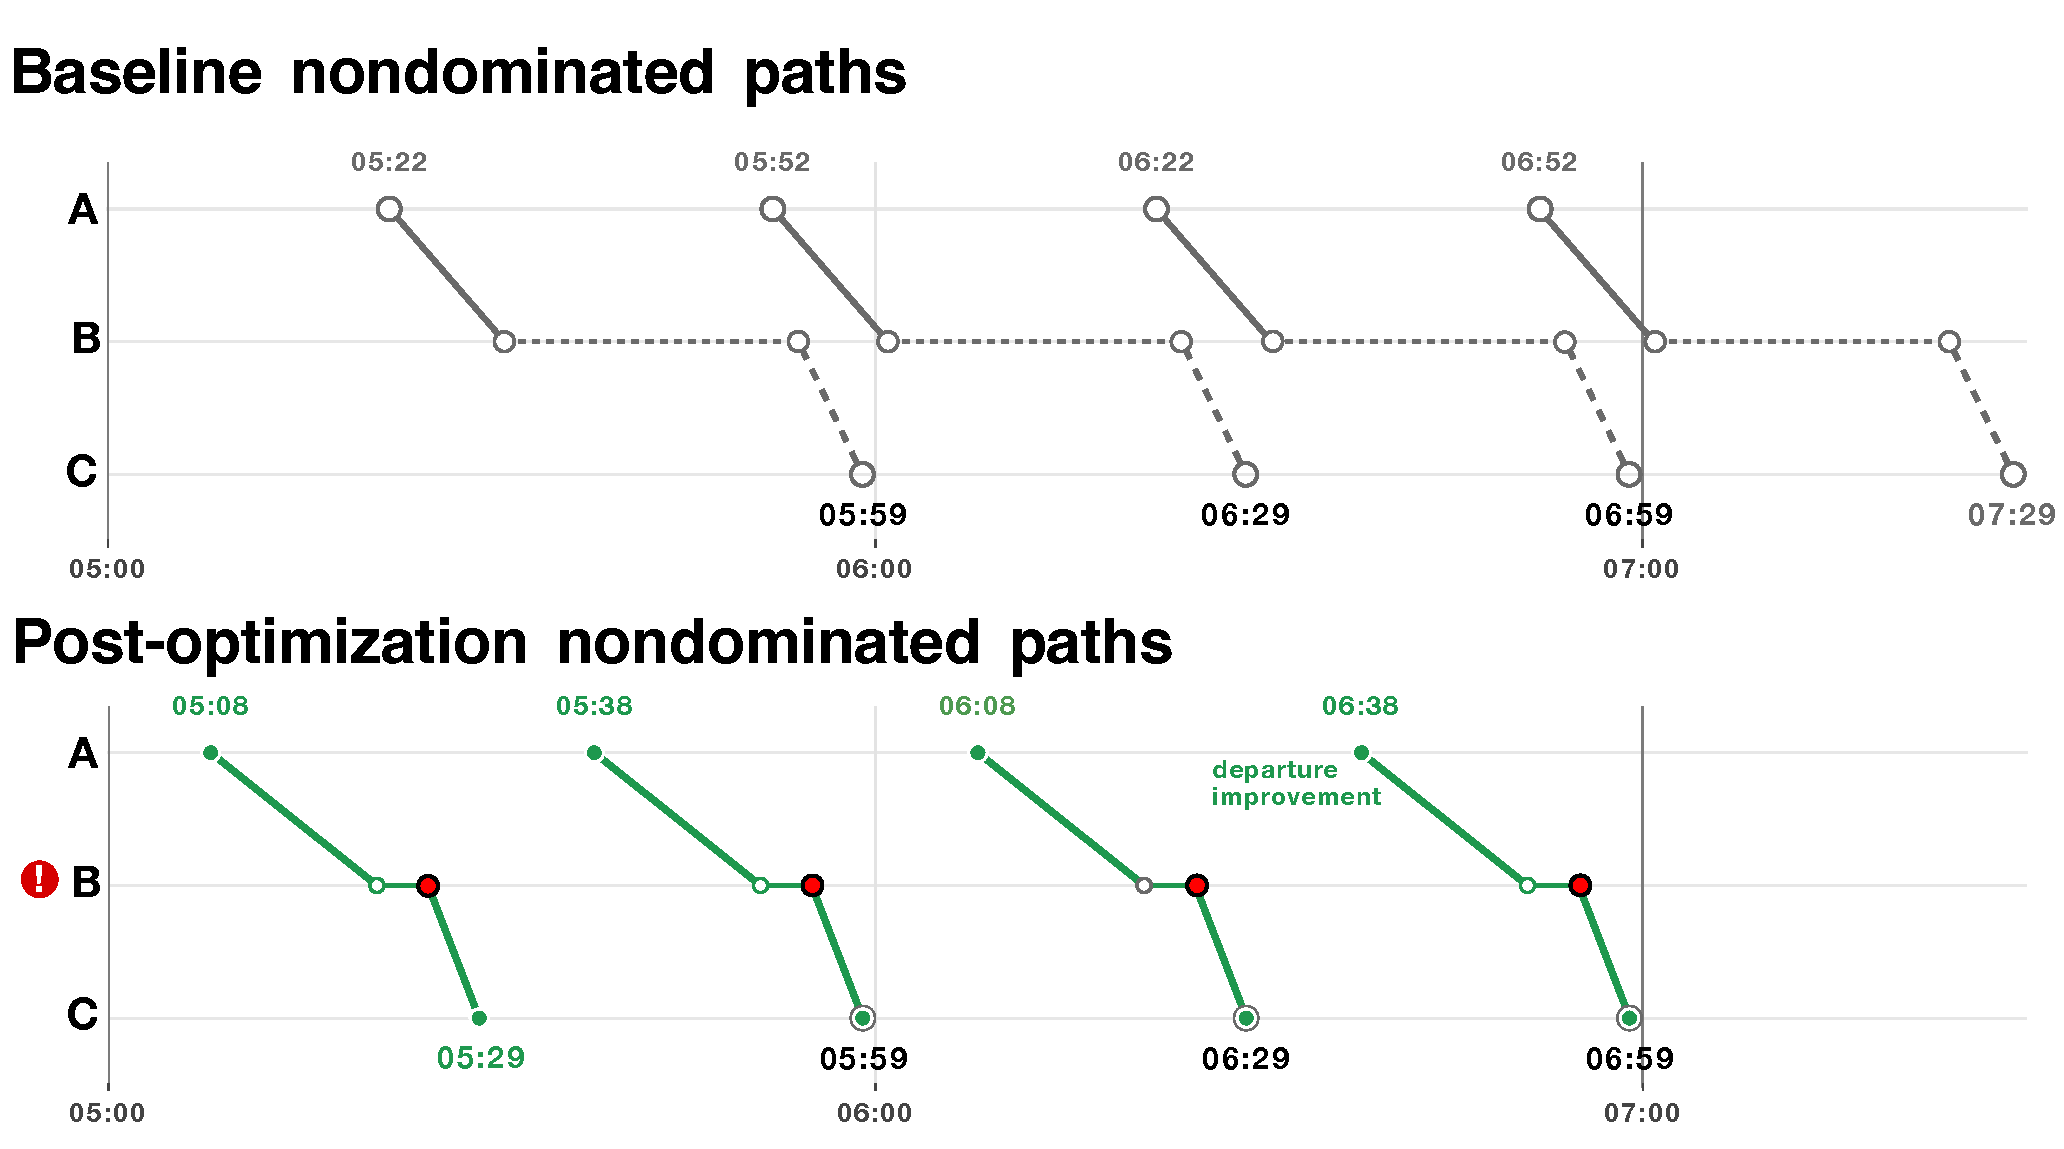
\includegraphics[
    width=\textwidth,
    height=0.29\textheight,
    keepaspectratio
]{figures/part-II/part2_od_extreme_paths_step3_2035EXPLANATION}
\end{center}

\noindent\textbf{Simplified version}



\begin{center}
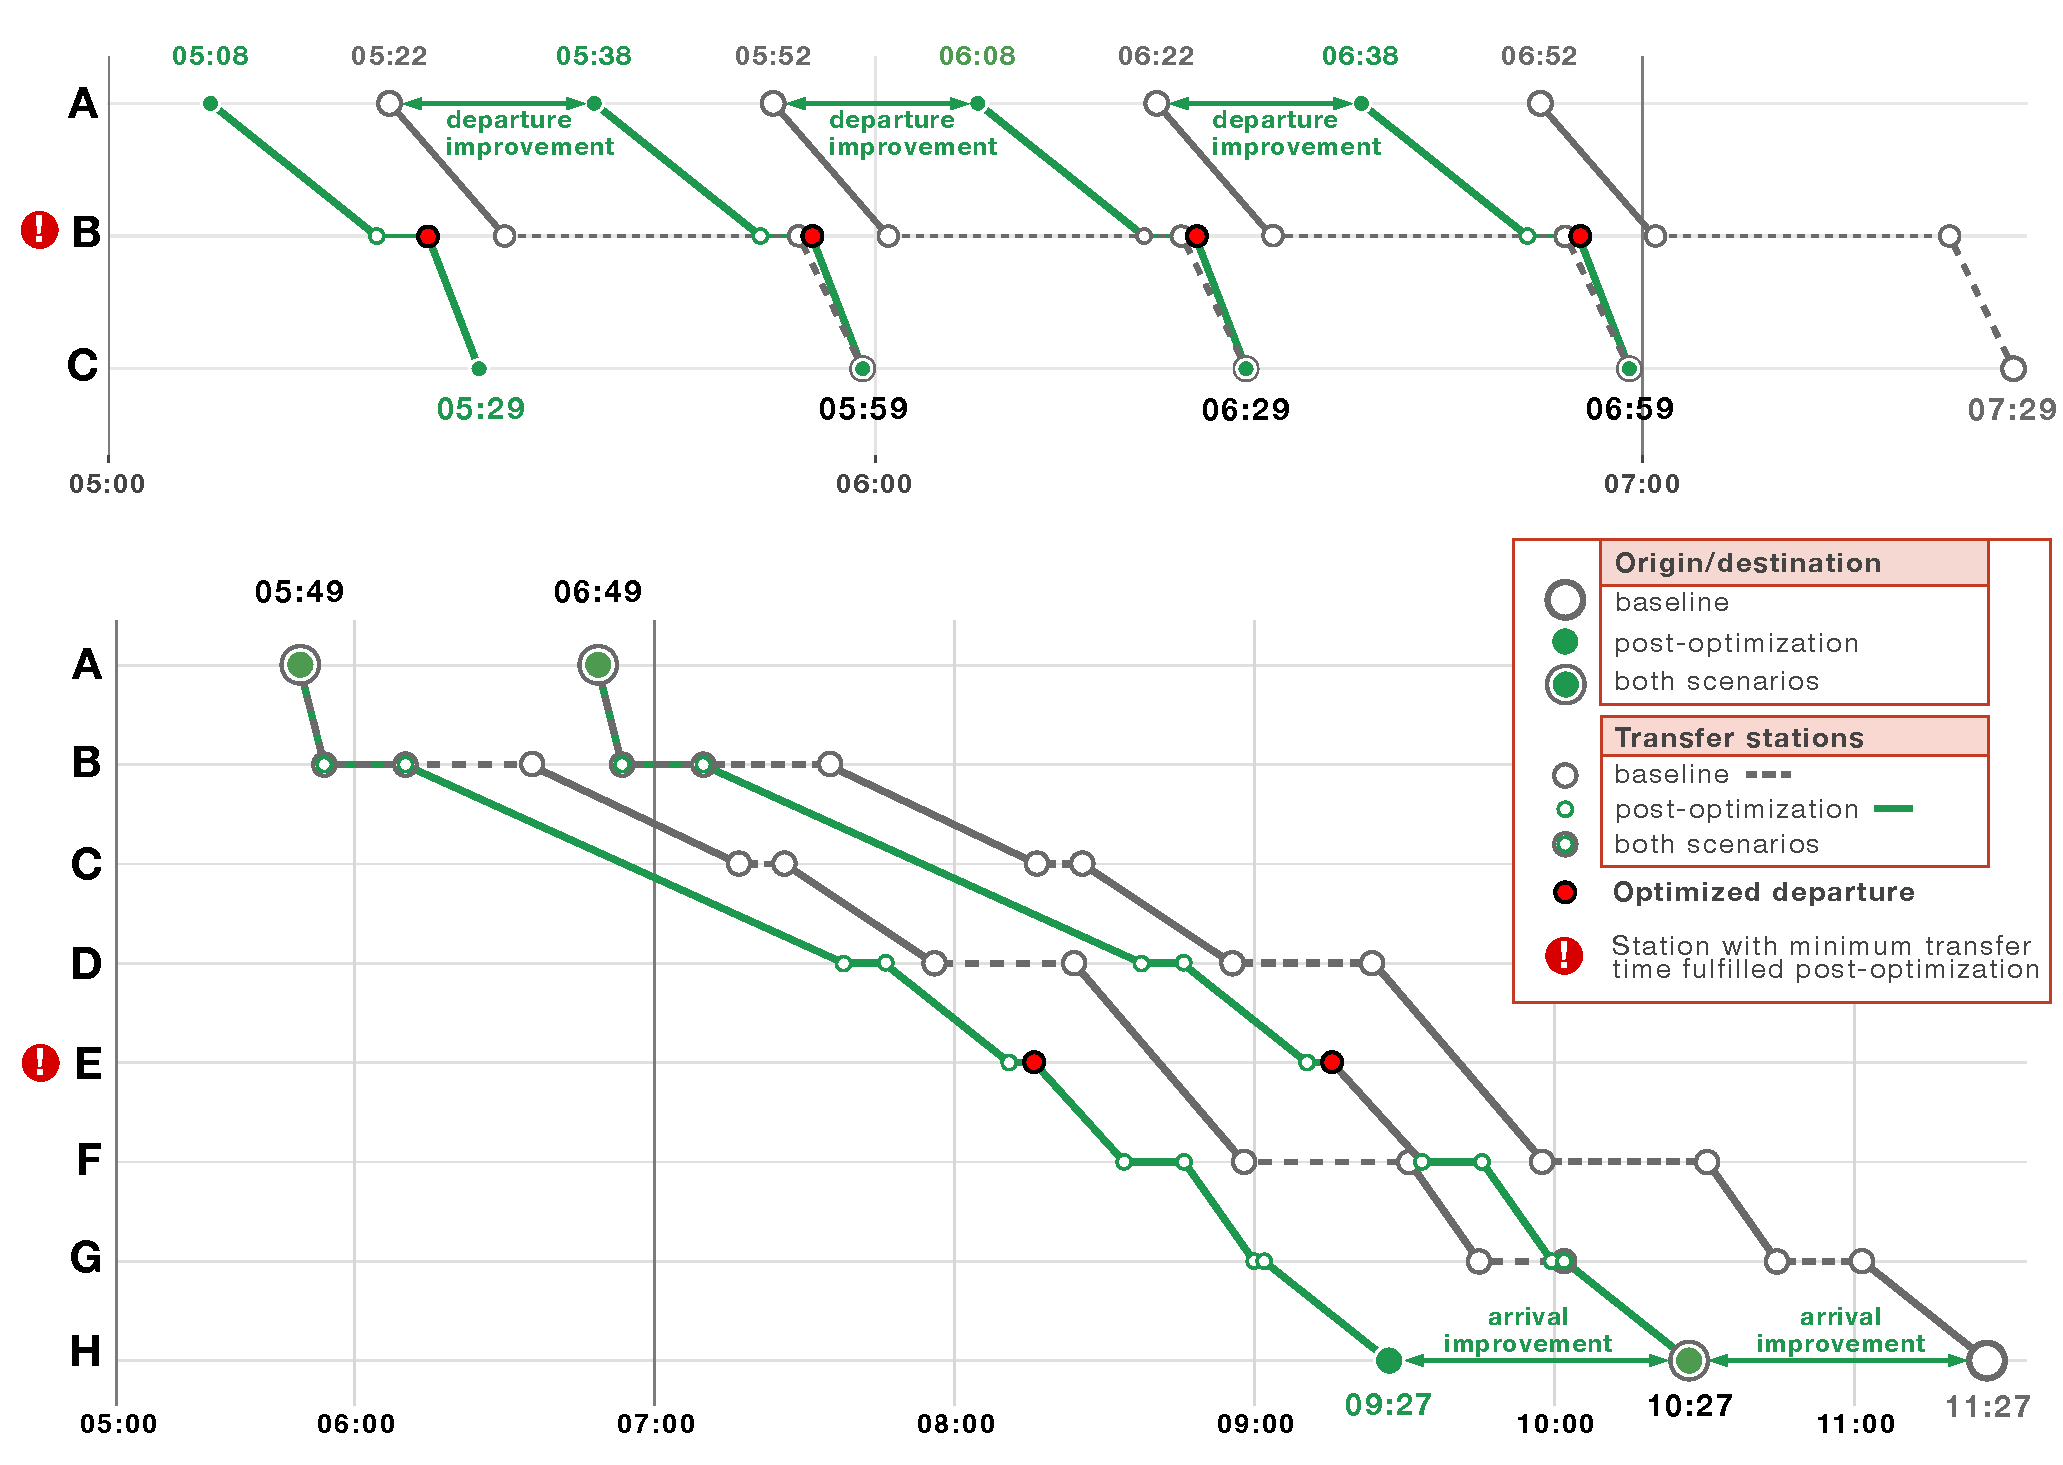
\includegraphics[
    width=\textwidth,
    height=0.39\textheight,
    keepaspectratio
]{figures/cover/part2_od_extreme_paths_step3_2035EASYTITLE.pdf}
\end{center}

\newpage
\noindent\textbf{Full version}


\begin{center}
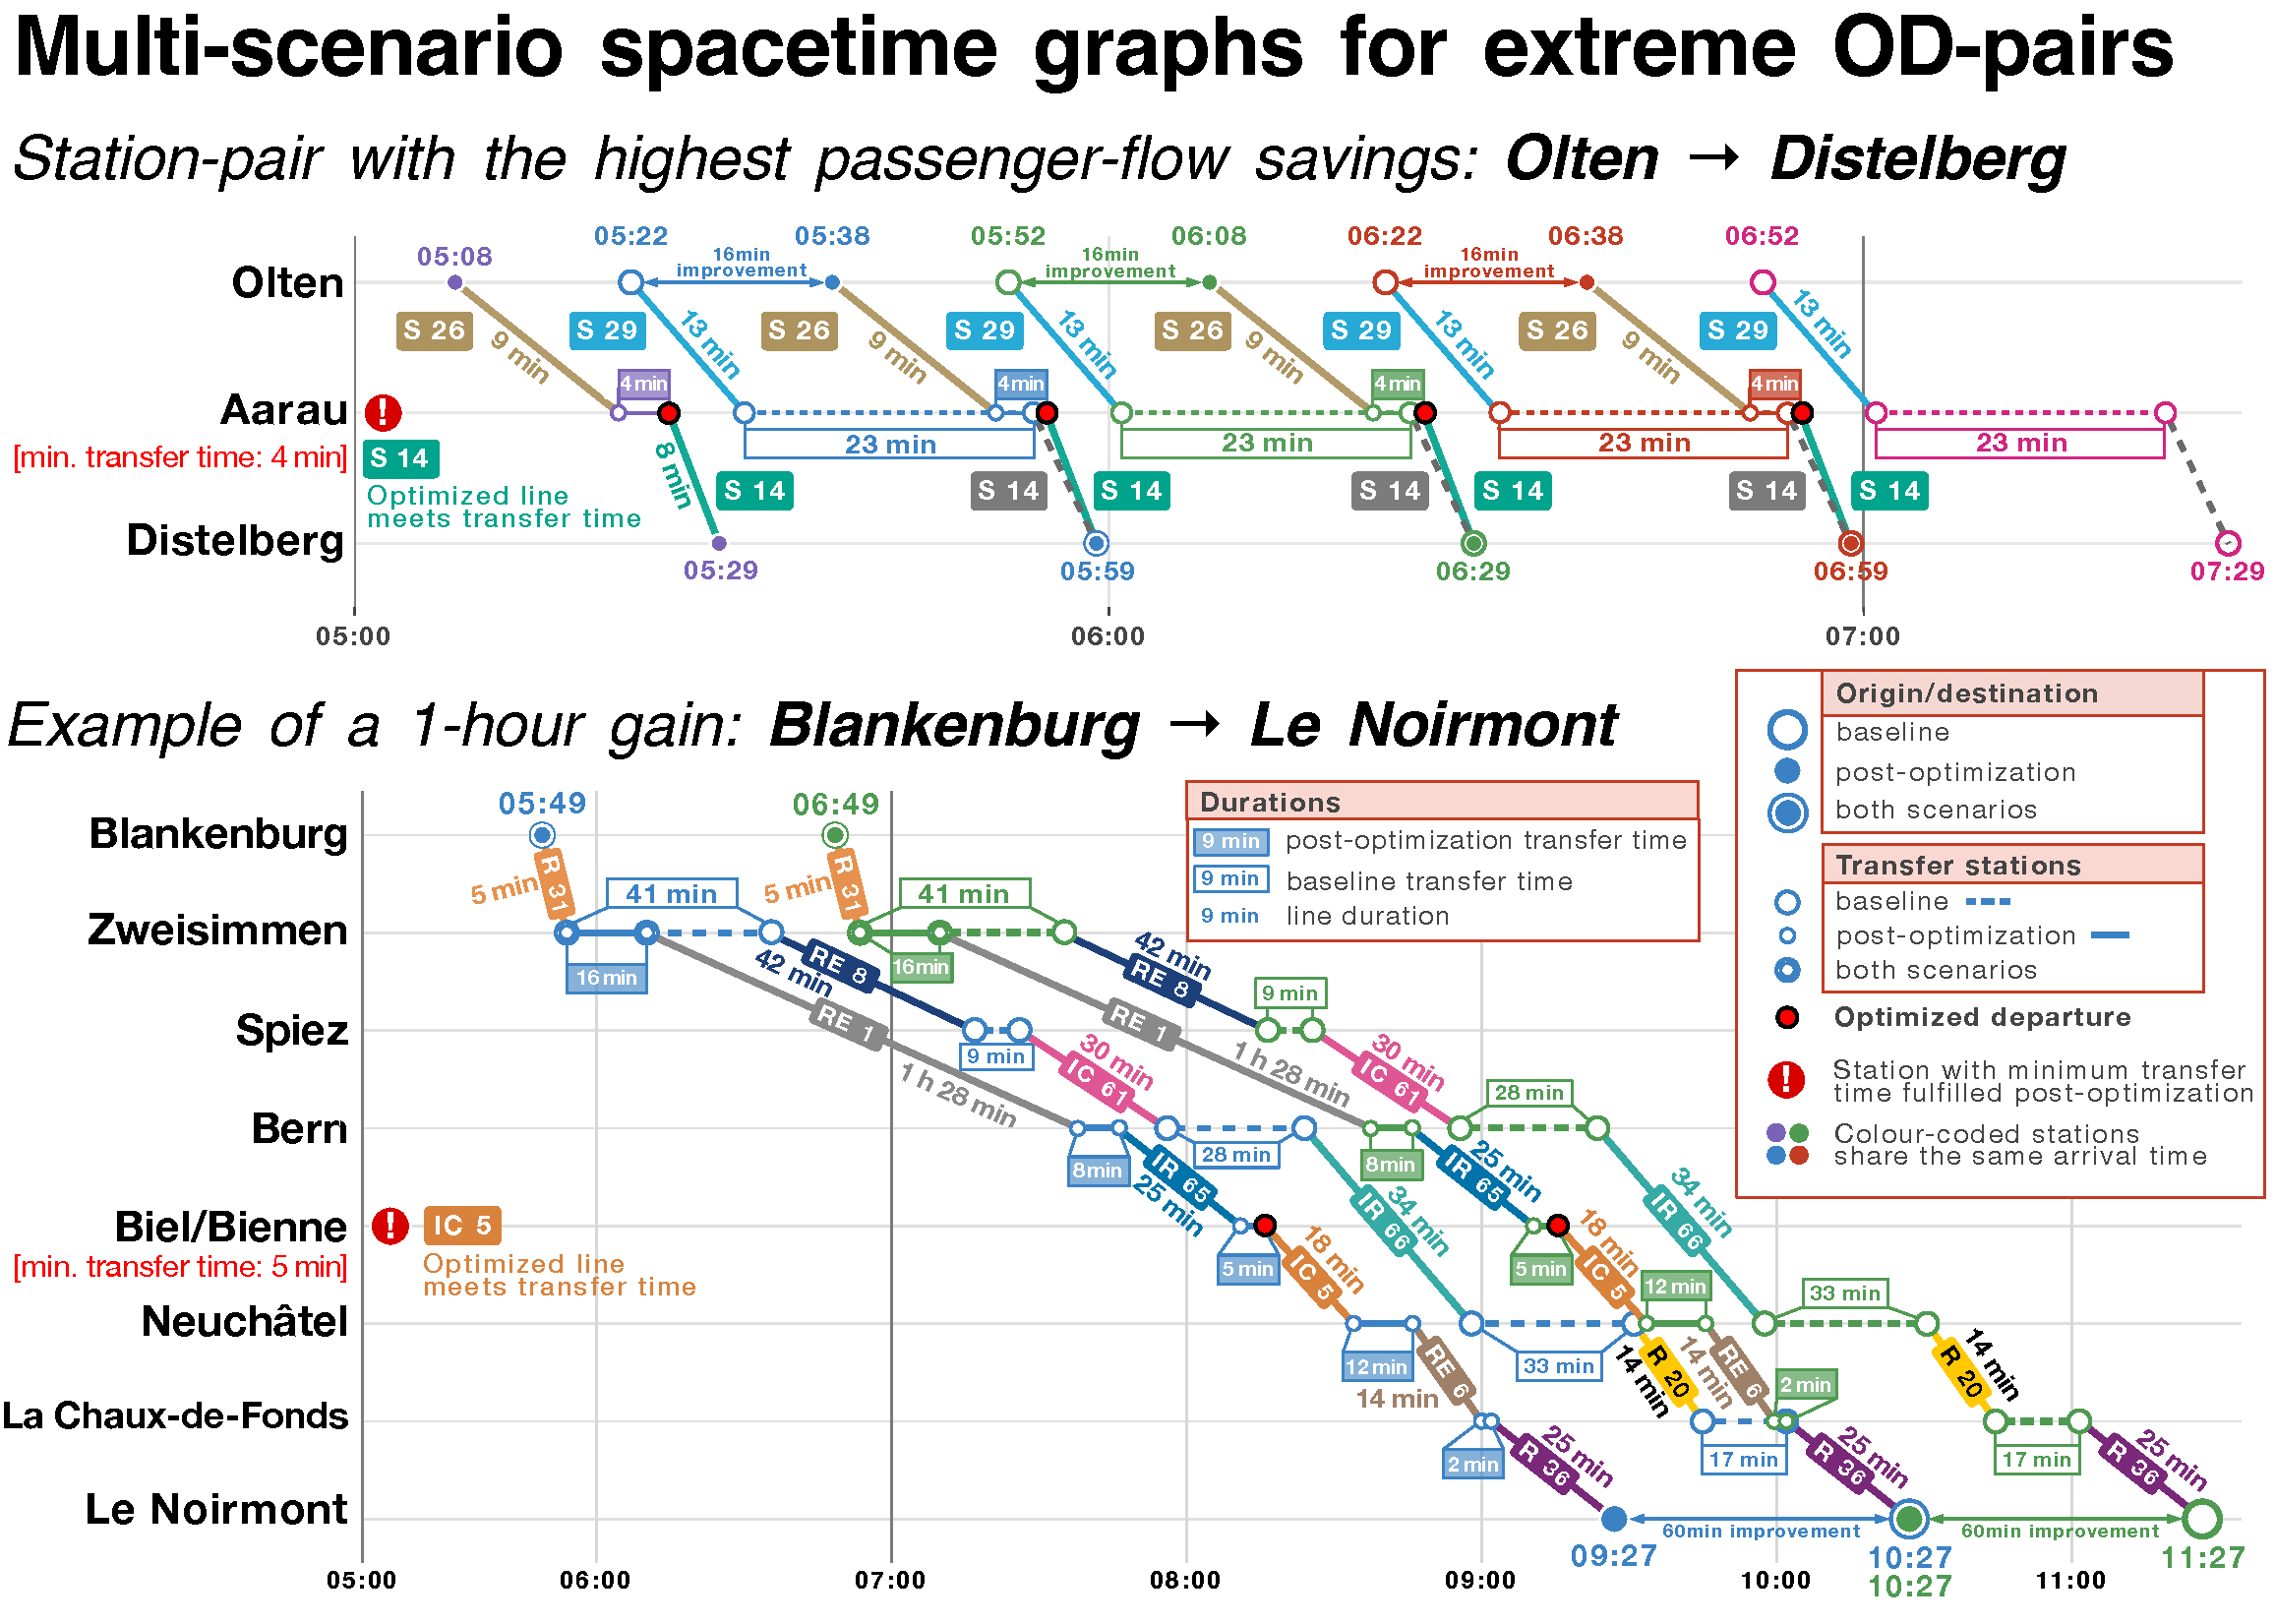
\includegraphics[
    width=\textwidth,
    height=0.39\textheight,
    keepaspectratio
]{figures/part-II/part2_od_extreme_paths_step3_2035.pdf}
\end{center}

\restoregeometry
\clearpage


\clearpage
\phantomsection
\section*{Acknowledgements}
\addcontentsline{toc}{section}{Acknowledgements}

I would like to sincerely thank Prof. Dr. Francesco Corman for his expertise, thoughtful insight as to what lines of inquiry to pursue, and valuable feedback throughout the thesis. I am also deeply grateful to Viera Klasovitá for her exemplary supervision and thoughtful guidance on how best to structure the research and communicate the results.

\section*{Data Availability Statement}
\addcontentsline{toc}{section}{Data Availability Statement}

The thesis source, compact timetable and demand inputs, accepted-edit manifests, analysis and figure-generation code, aggregated results, and reproducibility documentation are available at \url{https://github.com/MaBeAnGa/SwissPeriodicTimetableOptimisation}.

The complete routed scenario matrices are excluded from the repository because of their size. Adding the JSON row states together with the CSV overviews of all four scenarios in both years requires 2.008~TB of storage space. Excluding these CSVs, the enriched JSON archives representing fully-detailed OD matrices for each scenario contain 286.182~GB for Baseline, 286.470~GB for Optimized Step~1, 286.393~GB for Optimized Step~2, and 287.267~GB for Optimized Step~3. The total for all scenarios is 1.146~TB, or 573.449~GB for only the baseline and Step~3. The complete scenario states and accompanying visualizer app files are available from the author on reasonable request if the requester provides a suitably sized USB drive or equivalent physical storage. When stored locally, these scenario-state files enable the full companion web-app functionality, including timetable queries and targeted analysis for arbitrary OD pairs and municipal/cantonal groupings beyond the summary outputs contained within this thesis.

\section*{Additional Information}
\addcontentsline{toc}{section}{Additional Information}

\textbf{Preferred citation.}
Andrews García, M. B. (2026). \textit{Periodic Timetable Modelling \& Matheuristic Event-Retiming Optimization of the Swiss Passenger Rail Network}. Master's thesis, Institute for Transport Planning and Systems, ETH Zürich, Zurich.

\textbf{Declaration of AI-assisted tools.}
OpenAI Codex GPT-5.5 Extra High was used throughout the thesis for coding assistance, debugging, code review and data-analysis support.

\textbf{Hardware.}
All computational experiments and analyses reported in this thesis were conducted on a 16-inch Apple MacBook Pro with a 10-core Apple M1 Max processor and 64~GB of RAM. All mentioned processing speeds refer to this hardware configuration.

\textbf{Competing interests.}
The author declares no competing interests.

\end{document}
